% This is a template for Ph.D. dissertations in the UCI format.
% 
% All fonts, including those for sub- and superscripts, must be 10
% points or larger.  Recommended sizes are 14-point for chapter
% headings, 12-point for the main body of text and figure/table
% titles, and 10-point for footnotes, sub- and super-scripts, and text
% in figures and tables.
%
% Notes: Add short title to figures, sections, via square brackets,
% e.g. \section[short]{long}.
%
\documentclass[12pt,fleqn]{ucithesis}

% A few common packages
\usepackage{amsmath}
\usepackage{amsthm}
\usepackage{array}
\usepackage{graphicx}
\usepackage{natbib}
\usepackage{relsize}

% Some other useful packages
\usepackage{caption}
\usepackage{subcaption}  % \begin{subfigure}...\end{subfigure} within figure
\usepackage{multirow}
\usepackage{tabularx}

\usepackage[version=3]{mhchem}
\usepackage[T1]{fontenc}
\usepackage[table,xcdraw]{xcolor}
\usepackage{xr-hyper}
%\usepackage{hyperref}
\usepackage{float}
\usepackage{minted}
\usemintedstyle{monokai}
\definecolor{bg}{HTML}{282828}
\setminted{bgcolor=gray}

\makeatletter
\newcommand\aepath[1]{%%
  \bgroup
    \ttfamily
    \ae@path#1\relax\@nil
  \egroup}
\def\ae@path#1#2\@nil{%%
  \def\ae@continue{}%%
  \detokenize{#1}\unskip\penalty\z@  
  \ifx\relax#2%%
  \else 
    \def\ae@continue{\ae@path#2\@nil}%%
  \fi
  \ae@continue}
\makeatother

\let\texttt\aepath

\providecommand{\tightlist}{%
  \setlength{\itemsep}{0pt}\setlength{\parskip}{0pt}}

% plainpages=false fixes the "duplicate ignored" error with page counters
% Set pdfborder to 0 0 0 to disable colored borders around PDF hyperlinks
\usepackage[plainpages=false,pdfborder={0 0 0}]{hyperref}

% Uncomment the following two lines to use the algorithm package,
% which provides an algorithm environment similar to figure and table
% ("\begin{algorithm}...\end{algorithm}"). A list of algorithms will
% automatically be added in the preliminary pages. Note that you
% probably want a package for the actual code to go with this (e.g.,
% algorithmic).
%\usepackage{algorithm}
%\renewcommand{\listalgorithmname}{\protect\centering\protect\Large LIST OF ALGORITHMS}

% Uncomment the following line to enable Unicode support. This will allow you
% to enter non-ASCII characters (such as accented characters) directly without
% having to use LaTeX's awkward escape syntax (e.g., \'{e})
% NOTE: You may have to install the ucs.sty package for this to work. See:
% http://www.unruh.de/DniQ/latex/unicode/
\usepackage[utf8x]{inputenc}

% Uncomment the following to avoid "widowing", where page breaks cause
% single lines of paragraphs to float onto the next page (this is not
% a UCI requirement but more of an aesthetic choice).
%\widowpenalty=10000
%\clubpenalty=10000

% Modify or extend these at will.
\newtheorem{theorem}{\textsc{Theorem}}[chapter]
\newtheorem{definition}{\textsc{Definition}}[chapter]
\newtheorem{example}{\textsc{Example}}[chapter]
\newcommand{\angstrom}{\mbox{\normalfont\AA}}


% Macros for title, author, abstract, etc.
\thesistitle{Molecular simulations and binding free energy calculations for drug discovery}

%"Dissertation" for PhD, "Thesis" for master's
\documenttitle{Dissertation}

\degreename{Doctor of Philosophy}

% Use the wording given in the official list of degrees awarded by UCI:
% http://www.rgs.uci.edu/grad/academic/degrees_offered.htm
\degreefield{Pharmacological Sciences}

% Your name as it appears on official UCI records.
\authorname{Nathan M. Lim}

% Use the full name of each committee member.
\committeechair{David L. Mobley}
\othercommitteemembers
{
  Thomas L. Poulos\\
  Douglas J. Tobias
}

\degreeyear{2019}

\copyrightdeclaration
{
  {\copyright} {\Degreeyear} \Authorname
}

% If you have previously published parts of your manuscript, you must list the
% copyright holders; see Section 3.2 of the UCI Thesis and Dissertation Manual.
% Otherwise, this section may be omitted.
\prepublishedcopyrightdeclaration
{
	Chapter 1 {\copyright} 2016 American Chemical Society \\
	Chapter 2 {\copyright} 2018 Springer US \\
	All other materials {\copyright} {\Degreeyear} \Authorname
}

% The dedication page is optional
% (comment out to exclude).
% \dedications
% {
%   (Optional dedication page)
  
%   To ...
% }

\acknowledgments
{
Financial support was provided by the National Science Foundation Graduate Research Fellowship (DGE-1321846) and the Molecular Sciences Software Institute (MolSSI) Software Fellowship (ACI-1547580).
%Acknowledge GreenPlanet and TSCC compute time?
}


% Some custom commands for your list of publications and software.
\newcommand{\mypubentry}[3]{
  \begin{tabular*}{1\textwidth}{@{\extracolsep{\fill}}p{4.5in}r}
    \textbf{#1} & \textbf{#2} \\ 
    \multicolumn{2}{@{\extracolsep{\fill}}p{.95\textwidth}}{#3}\vspace{6pt} \\
  \end{tabular*}
}
\newcommand{\mysoftentry}[3]{
  \begin{tabular*}{1\textwidth}{@{\extracolsep{\fill}}lr}
    \textbf{#1} & \url{#2} \\
    \multicolumn{2}{@{\extracolsep{\fill}}p{.95\textwidth}}
    {\emph{#3}}\vspace{-6pt} \\
  \end{tabular*}
}

% Include, at minimum, a listing of your degrees and educational
% achievements with dates and the school where the degrees were
% earned. This should include the degree currently being
% attained. Other than that it's mostly up to you what to include here
% and how to format it, below is just an example.
%
% CV is required for PhD theses, but not Master's
% comment out to exclude
\curriculumvitae
{

\textbf{EDUCATION}
  
  \begin{tabular*}{1\textwidth}{@{\extracolsep{\fill}}lr}
    \textbf{Doctor of Philosophy in Pharmaceutical Sciences} & \textbf{2019} \\
    \vspace{6pt}
    University of California, Irvine & \emph{Irvine, CA} \\
    \textbf{Masters of Science in Pharmaceutical Sciences} & \textbf{2017} \\
    \vspace{6pt}
    University of California, Irvine & \emph{Irvine, CA} \\
    \textbf{Bachelor of Science in Pharmaceutical Sciences} & \textbf{2014} \\
    \vspace{6pt}
    University of California, Irvine & \emph{Irvine, CA} \\
  \end{tabular*}

\vspace{12pt}
\textbf{RESEARCH EXPERIENCE}

  \begin{tabular*}{1\textwidth}{@{\extracolsep{\fill}}lr}
    \textbf{Graduate Researcher} & \textbf{Sept 2014--Sept 2019} \\
    \vspace{6pt}
    University of California, Irvine & \emph{Irvine, California} \\
  \end{tabular*}
  \begin{tabular*}{1\textwidth}{@{\extracolsep{\fill}}lr}
    \textbf{Scientific Developer Intern} & \textbf{Jun 2015--Aug 2015} \\
    \vspace{6pt}
    Schrodinger, LLC. & \emph{New York, NY} \\
  \end{tabular*}
   \begin{tabular*}{1\textwidth}{@{\extracolsep{\fill}}lr}
    \textbf{Scientific Developer Intern} & \textbf{Jun 2014--Sept 2014} \\
    \vspace{6pt}
    Schrodinger, LLC. & \emph{New York, NY} \\
  \end{tabular*} 
   \begin{tabular*}{1\textwidth}{@{\extracolsep{\fill}}lr}
    \textbf{Undergraduate Researcher} & \textbf{Mar 2013--Sept 2014} \\
    \vspace{6pt}
    Mobley Lab, UCI Dept. of Pharma.Sci. & \emph{Irvine, CA} \\
  \end{tabular*}
   \begin{tabular*}{1\textwidth}{@{\extracolsep{\fill}}lr}
    \textbf{Undergraduate Researcher} & \textbf{Mar 2013--Jun 2014} \\
    \vspace{6pt}
    Poulos Lab, UCI Dept. of Pharma.Sci. & \emph{Irvine, CA} \\
  \end{tabular*} 

\vspace{12pt}  
\textbf{MENTOR EXPERIENCE}

    \mypubentry{Meghan Osato}{July 2017--Present}{Undergraduate--Biological Sciences \& Computer Science, Spring 2018 UROP Fellowship Awardee}
    \mypubentry{Linh P. Nguyen}{Sept 2016--June 2019}{Undergraduate--Pharmaceutical Sciences, Co-authored 2 Publications} 
  
\pagebreak

\vspace{12pt}
\textbf{PUBLICATIONS}
\begin{enumerate}
    \item \textbf{Lim, N.M.}; Osato, M.; Warren, G.; Mobley, D.L.
        \textit{Fragment pose prediction using non-equilbrium candidate monte carlo and molecular dynamics simulations.}
        In Preparation.
    \item Nguyen, L.P.$^*$; \textbf{Lim, N.M.$^*$}; Warren, G.; Mobley, D.L.
        \textit{Microsecond molecular dynamics simulations for fragment pose prediction.}
        In Preparation.
    \item Nainar, S.; Cuthbert, B.; \textbf{Lim, N.M.}; England, W.; Sophal, K.; Quechol, R.; Mobley, D.L.; Goulding, C.; Spitale, R.C. 
        \textit{An Optimized Chemical-Genetic Method for Cell-Specific Metabolic Labeling of RNA.}
        Submitted 2019 to Nature Methods
    \item Jandova, Z.; Gill, S. C.; \textbf{Lim, N.M.}; Mobley D.L.; and Oostenbrink, C.
        \textit{Binding modes and metabolism of caffeine}
        Submitted 2019 to Journal of Chemical Research and Toxicology
    \item Burley, K.H.; Gill, S.C.; \textbf{Lim, N.M.}; Mobley, D.L.
        \textit{Enhancing Sidechain Rotamer Sampling Using Non-Equilibrium Candidate Monte Carlo.}
        Journal of chemical theory and computation, 15(3), 1848-1862. 2019.
    \item Mobley, D.L.; Bannan, C.C.; Rizzi, A.; Bayly, C.I.; Chodera, J.D.; Lim, V.T.; \textbf{Lim, N.M.}; Beauchamp, K.A.; Slochower, D.R.; Shirts, M.R.; Gilson, M.K.
        \textit{Escaping Atom Types in Force Fields Using Direct Chemical Perception.}
        Journal of Chemical Theory and Computation, 14(11), 6076-6092. 2018.
    \item Gill, S; \textbf{Lim, N.M.}; Grinaway, P.; Rustenburg, A.S.; Fass, J.; Ross, G.; Chodera, J.D.; Mobley, D.L.
        \textit{Binding Modes of Ligands Using Enhanced Sampling (BLUES): Rapid Decorrelation of Ligand Binding Modes Using Nonequilibrium Candidate Monte Carlo.}
        Journal of Chemical Theory and Computation, 14(11), 6076-6092. 2018.
    \item Kyrychenko A.; \textbf{Lim, N.M.}; Freites, J.A.; Nguyen, L.P.; Tobias, D.J.; Mobley, D.L.
        \textit{Refining Protein Penetration into the Lipid Bilayer Using Fluorescence Quenching and Molecular Dynamics Simulations: The Case of Diphtheria Toxin Translocation Domain.}
        Journal of Membrane Biology, 251(3), 379-391. 2018.
    \item \textbf{Lim, N.M} 
        \textit{Molecular Dynamics Ligand FEP Tutorial August 2015}
        Schrödinger Academy, 2015.
    \item Holden, J.K.; Kang, S.; Hollingsworth, S.A.; Li, H.; \textbf{Lim, N.}; Chen, S.; Huang, H.; Xue, F.; Tang, W.; Silverman, R.B; Poulos, T.L.
        \textit{Structure-based design of bacterial nitric oxide synthase inhibitors.}
        Journal of Medicinal Chemistry, 58(2), 994-1004. 2015.
    \item Mobley, D.L.; Liu, S.; \textbf{Lim, N.M.}; Wymer, K.L.; Perryman, A.L.; Forli, S.; Deng, N.; Su, J.; Branson, K.; Olson. A.J.
        \textit{Blind prediction of HIV integrase binding from SAMPL4 challenge.}
        Journal of Computer Aided Molecular Design, 28(4):327-345. 2014.
    \item Mobley, D.L.; Wymer, K.L.; \textbf{Lim, N.M.}; Guthrie, J.P.
        \textit{Blind prediction of solvation free energies from the SAMPL4 challenge.}
        Journal of Computer Aided Molecular Design, 28:135-150. 2014.
    \item Holden, J.K.; \textbf{Lim, N.}; Poulos, T.L.
        \textit{Identification of Redox Partners and Development of a Novel Chimeric Bacterial Nitric Oxide Synthase for Structure Activity Analyses.}
        Journal of Biological Chemistry, 289(42): 29437-29445. 2014.
    \item Liu, S.; Wu, Y.; Lin, T.; Abel, R.; Redmann, J.; Summa, C.M.; Jaber, V.R.; \textbf{Lim, N.M.}; Mobley, D.L.
        \textit{Lead Optimization Mapper: Automating free energy calculations for lead optimization.}
        Journal of Computer Aided Molecular Design, 27(9):755-770. 2013. 
\end{enumerate}

\vspace{12pt}
\textbf{CONFERENCE PUBLICATIONS}

  \mypubentry{Sensitivity in binding free energies due to protein reorganization}{Aug 2016}{Theory and Applications of Computational Chemistry - Seattle}
  \mypubentry{Sensitivity in binding free energies due to protein reorganization}{Mar 2016}{American Chemical Society - San Diego}
  
\vspace{12pt}
\textbf{AWARDS}

  \mypubentry{Phase-II (Investment)}{MolSSI Software Fellowship}
  {The Molecular Sciences Software Institute (MolSSI) provides funding for a set of prestigious fellowships that recognize advanced graduate students and postdocs pursuing the development of software infrastructure, middleware, and frameworks that will benefit the broader field of computational molecular sciences, including biomolecular and macromolecular simulation, quantum chemistry, and materials science. MolSSI Software Fellows receive specialized training in state-of-the- art software design principles and tools, and they engage in outreach and educational efforts organized by the MolSSI.}
  \mypubentry{Phase-I (Seed)}{MolSSI Software Fellowship}
  {“Seed” Fellowships: These six month Fellowships will give recipients the opportunity to work with scientists at the MolSSI in order to implement recommended best practices, putting the Fellow’s project on a firm foundation.}
  \mypubentry{Graduate Research Fellowship}{NSF}
  {The NSF Graduate Research Fellowship Program (GRFP) helps ensure the vitality of the human resource base of science and engineering in the United States and reinforces its diversity. The program recognizes and supports outstanding graduate students in NSF-supported science, technology, engineering, and mathematics disciplines who are pursuing research-based master's and doctoral degrees at accredited United States institutions.}
  
\vspace{12pt}
\textbf{SOFTWARE}

  \mysoftentry{BLUES}{https://github.com/nathanmlim/blues}
  {Applications of nonequilibrium candidate Monte Carlo (NCMC) to ligand binding mode sampling}
  \mysoftentry{OpenMM Orion}{https://github.com/oess/openmm_orion}
  {Cubes and Floes for using OpenMM in Orion}
  

}

% The abstract was previously limited to a maximum of 350 words, 
% but the UCI manual at https://etd.lib.uci.edu/electronic/td2e#2.2.1.
% currently does not indicate that there is any word limit for the abstract
\thesisabstract
{Early stage drug discovery would change dramatically if computational methods could accurately and quickly predict binding modes and affinities of compounds in advance of experiments.
Simulation based approaches like classical molecular dynamics (MD) simulations have gained traction as a useful tool for early stage drug discovery, as MD provides a full atomistic and dynamic view of the biological system of interest.
In principle, MD simulations can be a powerful tool for lead optimization as MD can provide knowledge of the ligand's binding mode, dynamics, and even binding affinity.
In order to accurately compute binding affinities or predict ligand binding modes, simulations must run long enough to capture the relevant biological event or sufficiently sample all the physically relevant conformations.
My research presents the development of new simulation approaches for accelerated sampling and demonstrates the use of non-equilibrium candidate Monte Carlo moves with MD simulations for predicting ligand binding modes to a pharmaceutically relevant target.
}

%%% Local Variables: ***
%%% mode: latex ***
%%% TeX-master: "thesis.tex" ***
%%% End: ***


% Add PDF document info fields
\hypersetup{
	pdftitle={Molecular simulations and binding free energy calculations for drug discovery},
	pdfauthor={Nathan M. Lim},
	pdfsubject={Pharmaceutical Sciences},
	colorlinks,
    linkcolor={black!50!black},
    citecolor={blue!80!black},
    urlcolor={blue!80!black}
}

% Uncomment the following to have numbered subsubsections (by default
% numbering goes only to subsections).
%\setcounter{secnumdepth}{4}


% Set this to only select a subset of the includes directives below.
% Very handy to speed up compilation if you're working on a certain
% part of your thesis. It conserves page numbers, references, etc.
% even for non-included files.
%\includeonly{chapter1}

\begin{document}

% Preliminary pages are always loaded (TOC, CV, etc.)
\preliminarypages

% Include the different components of your thesis, in separate files.
% Using \include allows you to set \includeonly above.
\chapter*{Introduction} \label{introduction}

In recent years, molecular dynamics (MD) simulations has become an increasingly valuable tool in the pharmaceutical drug discovery process.
With the capability of providing a dynamic and complete atomistic viewpoint of a protein and bound ligand, it is no surprise that MD simulations are becoming routine in the development process.
Using MD simulations, chemists can gain knowledge of a ligand's binding mode(s), dynamics, and even binding affinity--making it an extremely powerful tool.
But, the accuracy in computed binding affinities and predictive capabilities for identifying ligand binding modes hinges on sufficient sampling of all relevant confirmations and biological motions. 

Often, sufficient sampling requires running extremely long simulations in order to capture biological motions as MD simulations resolve dynamics by taking small discrete timesteps (i.e 1-4 femtoseconds); whereas, biological motions often occur at the millisecond timescale.
Before the development of general purpose-graphic processing unit (GP-GPU) computing, MD simulations were largely bounded to simulations at the nanosecond timescale, but now microsecond timescales are becoming much more feasible with the use of GPUs.
Specialized hardware, like ANTON, has even been developed to make millisecond timescale simulations a reality.
Regardless, challenges in sampling of biological motions remains a challenge in the field as MD simulation often remained trapped in local energy minima--requiring longer timescales to escape before a new state can even be sampled.

Throughout this dissertation, I present my work which explores the use of MD simulations for the purpose of binding affinity calculations (Chapter \ref{RBFE}), studying membrane-protein insertion (Chapter \ref{DTT}), and ligand binding mode predictions (Chapter \ref{UCK2}, \ref{SEH-MD}, \ref{SEH-BLUES}).
Given, that MD simulations face challenges in sampling, I will also present my work in developing a software package which aims to accelerating sampling in ligand binding modes (Chapter \ref{BLUES}).

\section*{Summary}
Alchemical free energy perturbations (FEP) is one approach for computing binding affinities from MD simulations.
This approach works by `alchemically' (i.e. non-physical) modifying the ligand forces--taking it through a non-physical pathway--and computing the change in free energy throughout the process.
When combined with an enhanced sampling technique like replica exchange with solute tempering (REST), using an FEP+REST type of approach can provide accurate predictions in binding affinities.
Recently, this approach has been demonstrated to be successful in accurate calculations of binding free energies at large scales \cite{FEPplus}.
In Chapter \ref{RBFE}, I explore how sensitive calculated free energies are to small conformational changes in the protein using a simple model system with a congeneric series of small ligands.
In this study, I calculate relative binding free energies (RBFE) using the FEP+REST approach between the series of ligands bound to the commonly used model system of T4 lysozyme L99A.
Despite using an enhanced sampling approach, modifications to the enhanced sampling region (i.e. including a helix by the binding site) were required to get accurate free energy predictions which no longer depended on the starting conformation.
Here, my findings demonstrates the importance of sampling protein conformational changes in order to get accurate calculated binding free energies.

Before investigating ways to improve sampling with MD simulations, in Chapter \ref{DTT}, I use alchemical FEP calculations to study the membrane-protein insertion free energy of from diptheria toxin T domain (DTT).
This particular protein plays a role in the delivery of the diptheria toxin by facilitating the formation of a pore once inserted into a membrane.
In this study, I compute the differences in free energies when residue E362, located on the pore of the translocation domain, is charged and neutral via alchemical FEP calculations.
From the calculated free energies, I aimed to gain some insight on the importance of the particular residue and its charge state during the membrane insertion process.
Here, I found that the neutral state of the residue was significantly more favorable over the charged state during the insertion process and discovered the neutral state of the protein also facilitated formation of a larger pore--which supported experimental studies.

From Chapter \ref{RBFE}, I learned how critical it was to properly sample conformational states if I wanted to achieve accurate binding free energies.
Thus, in Chapter \ref{BLUES}, I co-developed a software package which aims to accelerate sampling of ligand binding modes.
This software package is called BLUES: Binding modes of Ligands Using Enhanced Sampling, which uses a hybrid simulation approach that combines non-equilbirum candidate Monte Carlo (NCMC) move proposals with MD simulations.
In this framework, we first implemented random rotational move proposals which are performed on the bound ligand.
By randomly rotating the ligand during simulations, the aim is to search for and sampling other binding modes; whereas, MD simulations often remain trapped in their initial binding mode.
In Chapter \ref{BLUES}, I discuss how to install and use the software, detail the functions and modules in the codebase, and provide an overview on design principles I had implemented to ensure the software can easily be maintained and extended beyond our initial implementation.
From my extensible design, several projects in the Mobley lab were able to use the BLUES framework and implement new NCMC move types beyond simple ligand rotations.
Some of these moves include sidechain rotations, ligand torsional rotations, and localized water motions which all enhance sampling in different ways than our initial implementation.
An application of the BLUES software for the purpose of predicting ligand binding modes is presented in Chapter \ref{SEH-BLUES}.

In the interest of using MD simulations for predicting ligand binding modes, in Chapter \ref{UCK2}, I present my work where I use MD simulations to identify ligand binding modes for various RNA nucleoside analogs which bind to the protein uridine cytidine kinase 2 (UCK2).
The Spitale lab had developed novel RNA nucleoside analogs which would become incorporated into the nascent RNA strands produced from UCK2.
They were interested in gaining some structural insights on how their analogs bound in the binding site of UCK2, in comparison to the endogenous ligand.
In this study, I utilize docking and molecular dynamics (MD) simulations to validate their hypothesis of their nucleoside analogs binding in the same binding mode as the endogenous ligand, cytidine, as well as uncover a novel binding mode, representative of the post-catalytic state of UCK2.
The predicted binding modes I had found via MD simulations were later validated by x-ray crystallography.
From this study, I developed a protocol to define the metastable binding modes sampled during the MD simulations using Markov State Models (MSM) construction and clustering.
Additionally, I demonstrate that computational methods like MD simulations can indeed be used to predict binding modes for this system.

In Chapter \ref{SEH-MD}, I present my work in using microsecond long MD simulations to predict binding modes for fragments which bind to a protein called soluble epoxide hydrolase (SEH).
Posed a retrospective blinded study, our collaborators at OpenEye Scientific Software provided us with a series of fragments and the SEH binding site to dock to.
Here, we use a combined docking-MD simulation approach and investigate if enough sampling of ligand binding modes can occur at the microsecond timescale and if the populations (i.e. \% simulation time) of the binding modes found would help us identify the dominant (crystallographic) binding mode and any additional binding modes. 
From this study, we found that even with microsecond long MD simulations, we did not observe sufficient transitions between binding modes and failed to identify the crystallographic binding modes.
This failure highlighted the need to use an enhanced sampling technique so as to acquire better sampling of ligand binding modes.

To address the failures from Chapter \ref{SEH-MD}, I revisit the study using the (NCMC+MD) BLUES approach for predicting the binding modes for the SEH fragments in Chapter \ref{SEH-BLUES}.
Here, I investigate if BLUES can be applicable beyond a simple model system, like T4 lysozyme L99A, and apply it to a system with pharmaceutical relevance--SEH.
Using BLUES, I observed significantly better sampling in ligand binding modes than with microsecond long MD simulations, which lead to better predictions of the SEH fragment binding modes.
From this study, I demonstrate that BLUES can indeed be used to accelerate binding mode sampling to more complex systems and illustrate that it can potentially be used as a tool for predicting fragment binding modes.


\chapter{Sensitivity in binding free energies due to protein reorganization} \label{RBFE}

\begin{center}
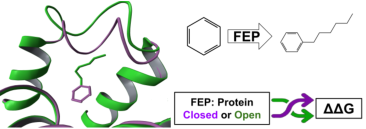
\includegraphics[width=9cm,height=3.5cm]{Figures/T4-L99A_cover.pdf} \\
\small{Authors: Nathan M. Lim, Lingle Wang, Robert Abel, and David L. Mobley}\\
\emph{J. Chem. Theory Comput., 2016, 12 (9), pp 4620--4631 \\
\doi{doi:10.1021/acs.jctc.6b00532}\\Publication Date (Web): July 27, 2016}

\end{center}

\section{Abstract}
Tremendous recent improvements in computer hardware, coupled with advances in sampling techniques and force fields, are now allowing protein-ligand binding free energy calculations to be routinely used to aid pharmaceutical drug discovery projects.
However, despite these recent innovations, there are still needs for further improvement in sampling algorithms to more adequately sample protein motion relevant to protein-ligand binding.
Here, we report our work identifying and studying such clear and remaining needs in the apolar cavity of T4 Lysozyme L99A.
In this study, we model recent experimental results that show the progressive opening of the binding pocket in response to a series of homologous ligands \cite{Merski2015}.
Even while using enhanced sampling techniques, we demonstrate that the predicted relative binding free energies (RBFE) are sensitive to the initial protein conformational state.
Particularly, we highlight the importance of sufficient sampling of protein conformational changes and demonstrate how inclusion of three key protein residues in the 'hot' region of the FEP/REST simulation improves the sampling and resolves this sensitivity.

\section{Introduction}
Proteins play a central role in many biological processes by modulating many key signaling pathways.
It is unsurprising to find that proteins make up the vast majority of pharmaceutical drug targets.
Many small-molecules on the market today induce their therapeutic effect by modulating the proteins' biological activity through binding\cite{overington2006many,FCP:FCP548,Lundstrom2009}.
Thus, optimization of protein-ligand binding affinities is a central goal in early pharmaceutical drug design projects.

Recent advancements in technology and computational chemistry have led to increasing use of computer-aided drug design techniques to assist in lead optimization in pharmaceutical drug discovery.
Since accuracy and reliability of the approach being used is critical for success, it is here where the most rigorous of methods like free energy calculations can be applied in the prediction of protein-ligand binding affinities.
Using alchemical methods like free energy perturbation (FEP), thermodynamic integration, and $\lambda$-dynamics on molecular dynamics (MD) simulations, the difference in binding free energies between two ligands can be computed in a robust and accurate manner.
By computing relative binding free energies, much of the computational cost and difficulties of absolute binding free energy calculations is avoided\cite{doi:10.1021/ct5000296,chipot2007free,chodera2011alchemical,knight2009lambda,zheng2008random,gallicchio2011advances,doi:10.1021/ct500161f}.
Other advancements in forcefields, sampling algorithms, and emergence of GPU computing have considerably improved the accuracy and robustness of alchemical calculations.
The recent development of FEP+, a fully automated alchemical protocol implemented with modern methodologies, reduces overall workload and the potential for human error in setup and analysis of these types of calculations.
Using this protocol, previous studies\cite{FEPplus} have demonstrated it to yield highly accurate free energy predictions in a wide range of pharmaceutically relevant protein targets and ligands.
The accuracy and reliability of FEP+ makes it a very powerful tool in the hands of medicinal chemists for efficient optimization of lead compounds.

Although the previous report on FEP+\cite{FEPplus} demonstrates its robustness, the primary concern focuses on the size of the ligand perturbation or the initial ligand pose and how these factors impact the accuracy of calculated free energies\cite{mobley2012perspective,doi:10.1021/acs.jctc.5b00214}.
Careful consideration of effects arising from protein conformational changes have generally received less attention due to the difficulty in addressing the sampling challenges encountered when simulating proteins.
The difficulty in protein sampling lies primiarly in the timescales required to adequately capture a complete biomolecular event.
Timescales of such events can range from nanoseconds to milliseconds (or even seconds)\cite{elber2005long}.
In MD simulations, the system evolves in time through series of short time steps (i.e. 2 fs) by repeatedely computing the forces on each individual atom in accordance to Newton's laws of motion at each time step.
Not only must a computer perform numerous calculations at each time step, but it must repeat this process an enourmous amount of times to generate a trajectory that is on timescale for your biological process of interest\cite{karplus2005molecular}.
Furthering the difficulty, with using `vanilla' MD simulations, the system will more than likely remain kinetically trapped in an energy minima, thereby preventing any further exploration of the protein conformational space and obtaining proper sampling.
Some computational studies have shown even small simple changes in the protein---like a side-chain rotamer flipping---can cause large errors in affinity predictions if not properly sampled\cite{Mobley2009489,Mobley20071118,Jiang:2010tg,Meng:2015gj}.
Overcoming these high energy barriers is no easy feat; whereby a number of distinct approaches like metadynamics\cite{laio2002escaping}, accelerated MD\cite{hamelberg2004accelerated}, and temperature accelerated MD\cite{Maragliano2006168} aim to solve this problem of kinetic traps but may fall short in some cases\cite{borhani2012future}.
Thus, careful sampling of protein conformational changes is critical for accurate and reliable affinity predictions.

In the previous FEP+ study\cite{FEPplus}, other than simply restricting ourselves to congeneric series with multiple reported crystal structures, no effort was made to either include or exclude cases where the protein or ligand binding mode may reorganize.
However, it is entirely possible some of the outliers reported in that work may be due to protein conformational reorganization.
The testing of the FEP+ technology on cases where protein reorganization has been well-characterized experimentally may provide an opportunity to probe potential pathological cases, and further provides an opportunity to discover how to further improve the technology. While some studies suggest protein reorganization on ligand binding can be relatively common (i.e. as reviewed by~\cite{Mobley:2009bm}), it is far from well understood how often this can be a challenge for binding prediction.
Regardless, it is clear that protein-ligand binding can be highly complex, and multiple stable protein conformations may be populated even for the same ligand \cite{doi:10.1021/jm060167o,Gutteridge200521,Merski2015}.
Thus, there is a great need to understand how protein conformational changes and the choice of starting protein conformation may affect the reliability of free energy predictions.

\begin{figure}[H]
\begin{subfigure}[t]{0.5\linewidth}
   \centering
   \caption{T4 lysozyme (L99A)}
   \label{fig:T4-L99A_protein}
   \frame{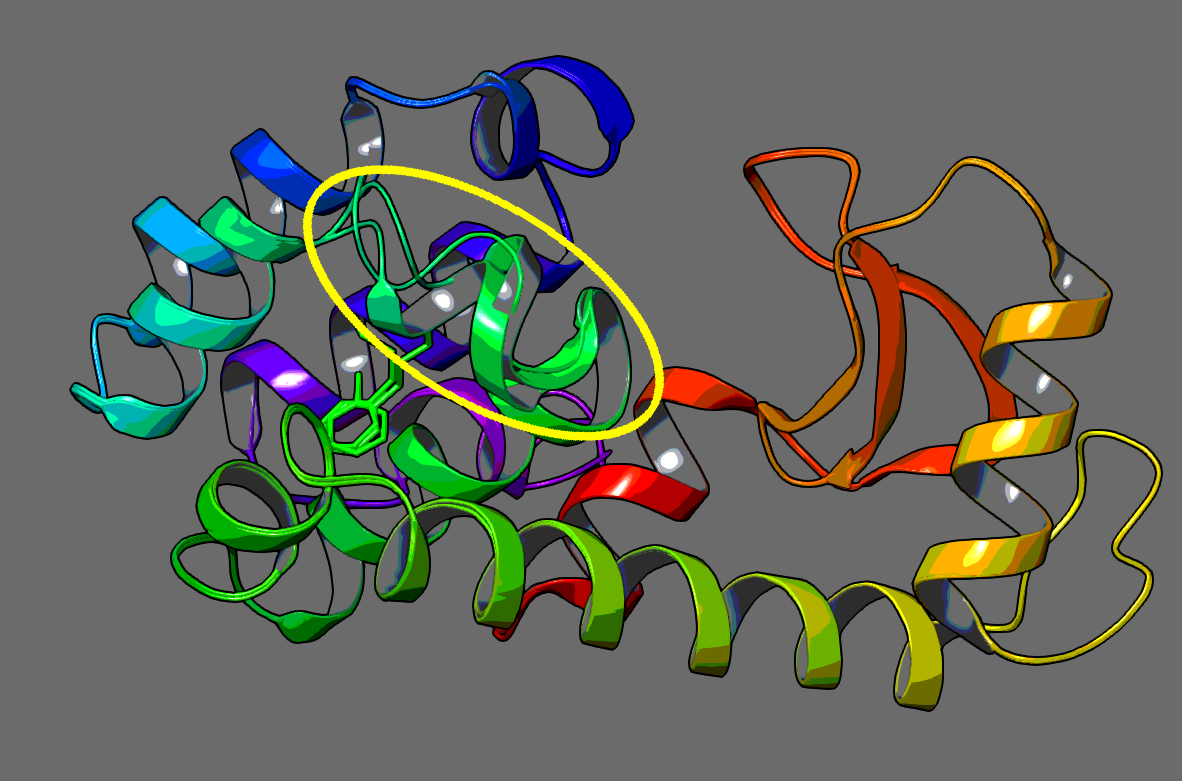
\includegraphics[clip, height=0.25\textheight, width=\linewidth]{Figures/Protein/T4_lysozyme_edit.png}}
\end{subfigure}\hfill
\centering
\begin{subfigure}[t]{0.5\linewidth}
  \centering
  \caption{F-helix (residues 107-115)}
  \label{fig:T4-L99A_tube}
  \frame{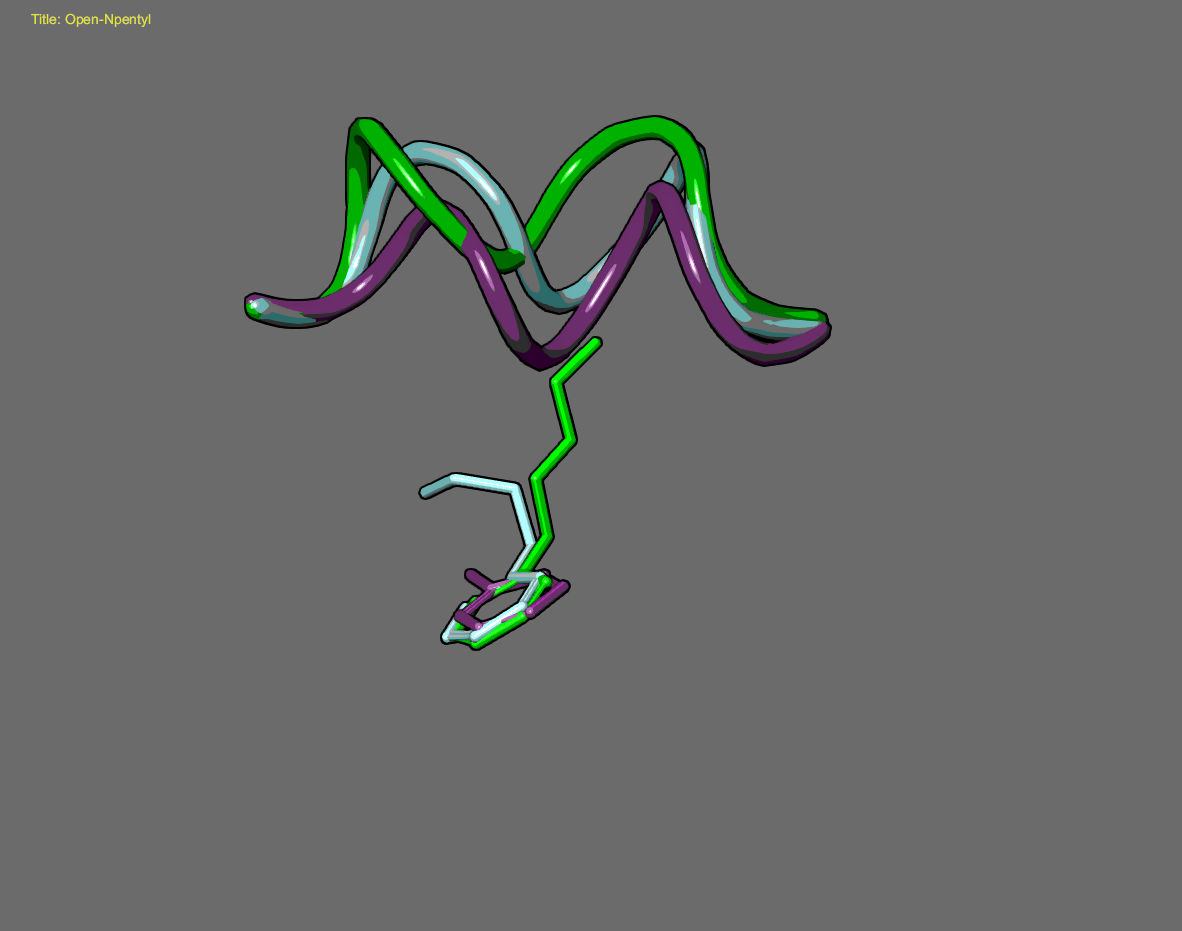
\includegraphics[trim={8cm 8cm 12cm 3cm}, clip, height=0.25\textheight, width=\linewidth]{Figures/Protein/ProteinTube.png}}
\end{subfigure}\hfill
\begin{subfigure}{0.30\textwidth}
   \centering
   \caption{Closed State}
   \label{fig:closed_surface}
   \frame{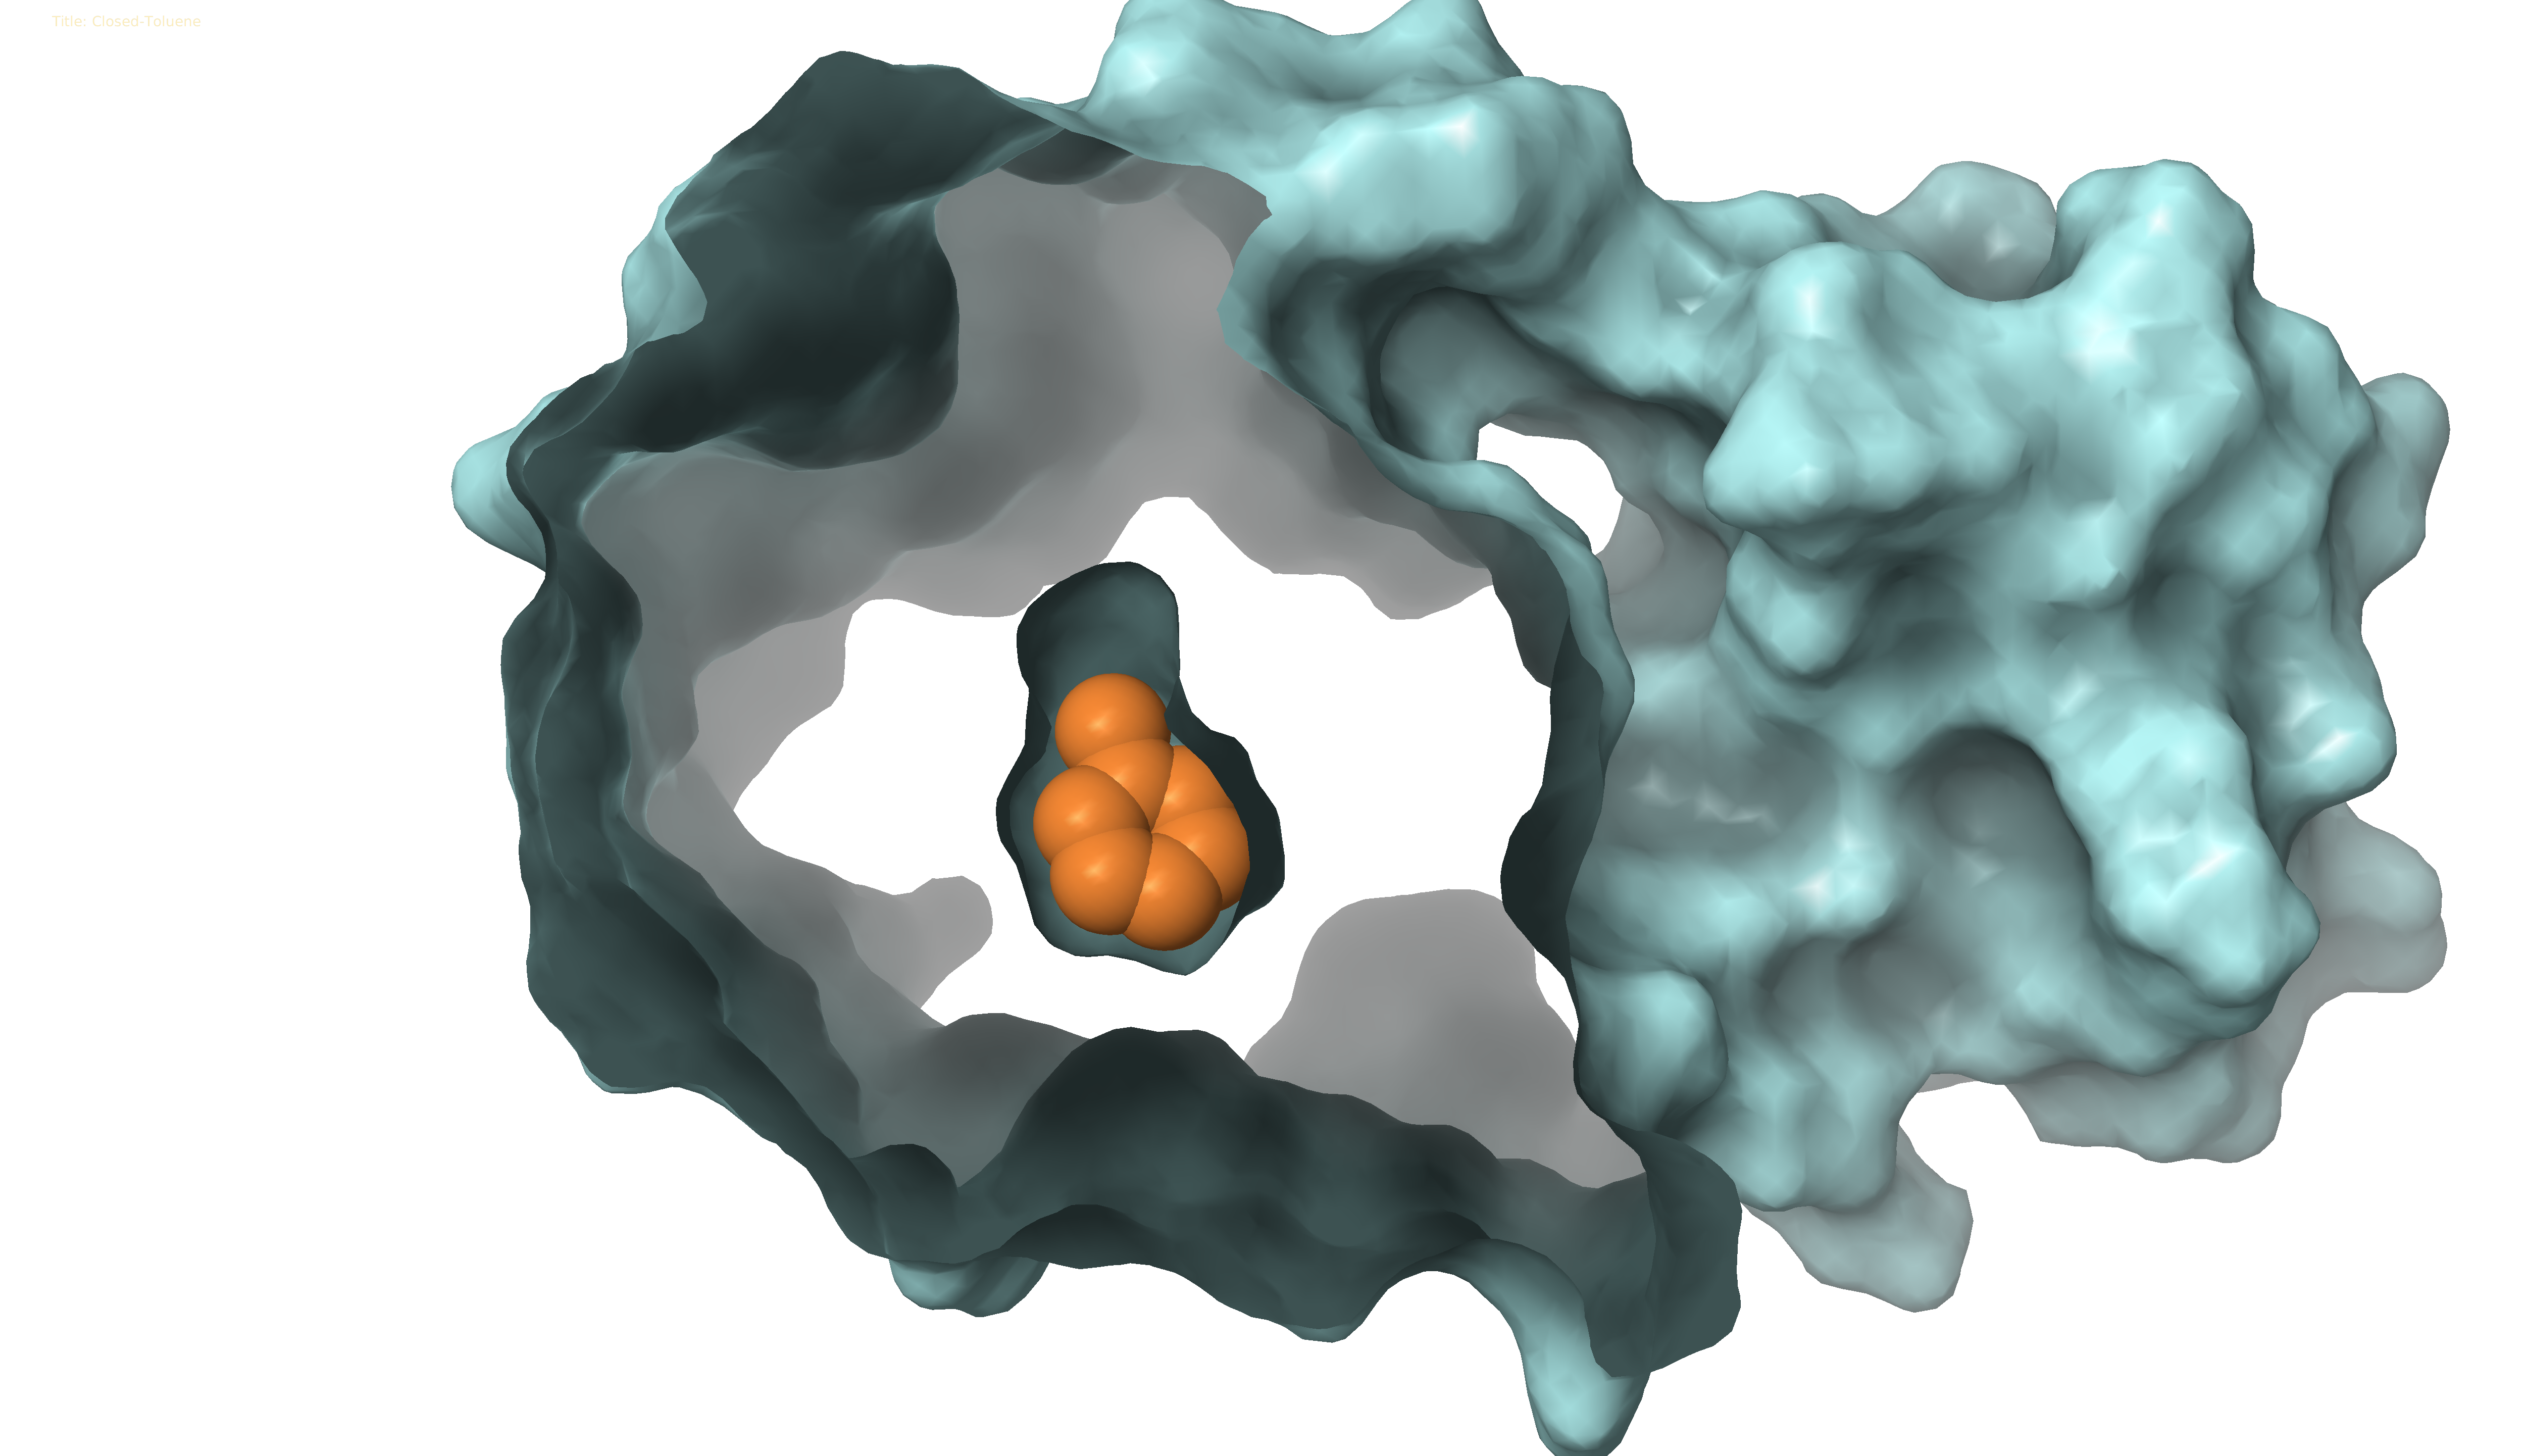
\includegraphics[trim={10cm 5cm 15cm 2cm}, clip, height=0.25\textheight]{Figures/Protein/closed_surface_trans.png}}
\end{subfigure}\hfill
\centering
\begin{subfigure}{0.30\textwidth}
  \centering
   \caption{Intermediate State}
   \label{fig:int_surface}
   \frame{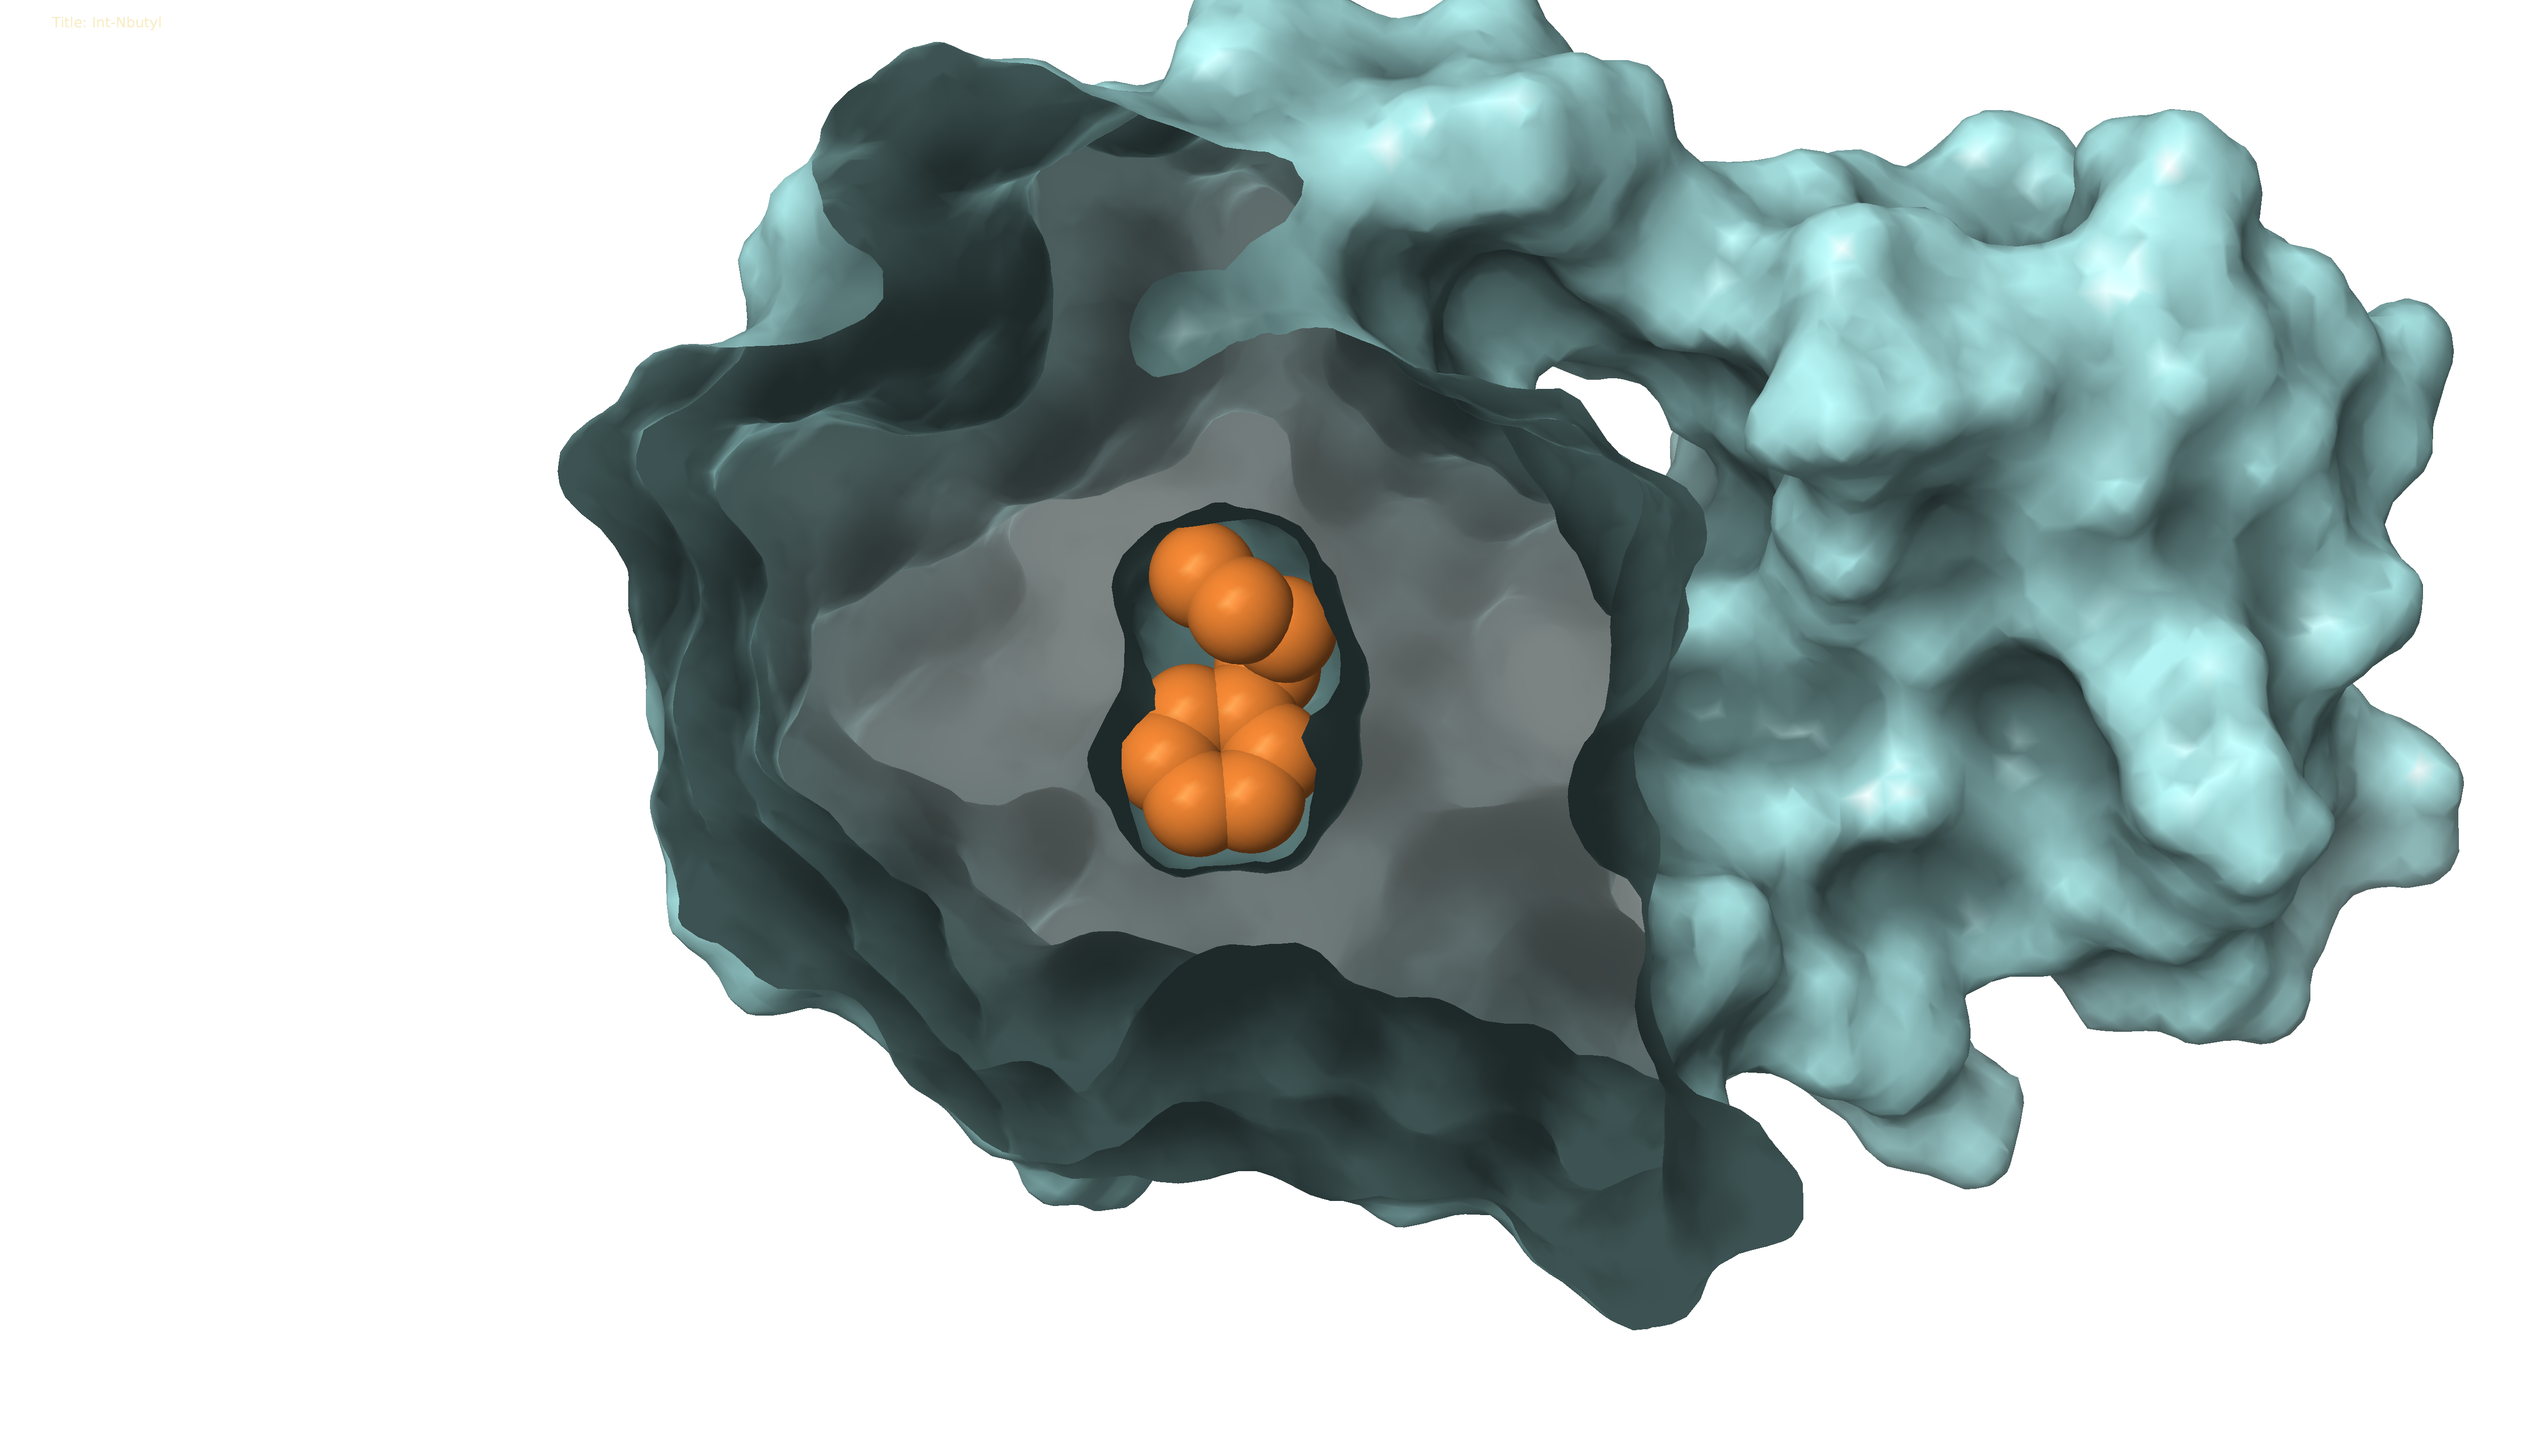
\includegraphics[trim={10cm 5cm 15cm 2cm}, clip, height=0.25\textheight]{Figures/Protein/int_surface_trans.png}}
\end{subfigure}\hfill
\centering
\begin{subfigure}{0.30\textwidth}
   \centering
   \caption{Open State}
   \label{fig:open_surface}
   \frame{\includegraphics[trim={5cm 5cm 15cm 2cm}, clip, width=\linewidth, height=0.25\textheight]{Figures/Protein/open_surface_trans.png}}
\end{subfigure}
\centering
\begin{subfigure}{0.75\textwidth}
   \centering
   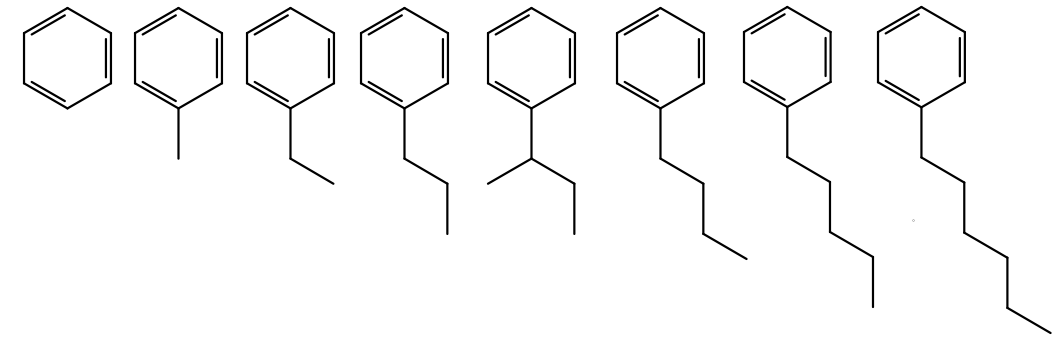
\includegraphics[clip, width=\textwidth, height=0.15\textheight]{Figures/Protein/ligand_set.png}
   \caption{Ligand Set}
   \label{fig:ligand_set}
\end{subfigure}\hfill
\caption[T4-L99A bound complexes]{In Fig.\ref{fig:T4-L99A_protein} are overlaid cartoon representations of T4 lysozyme using the protein-ligand bound crystal structures of the toluene(4W53), butylbenzene(4W57), and hexylbenzene(4W59) complexes where the F-helix region is highlighted in yellow.
Fig.\ref{fig:T4-L99A_tube} illustrates a closer view of strictly the F-helix in the closed(purple), intermediate(cyan), and open(green) conformational states and their corresponding ligands as found in the crystal structure.
Below are the molecular surface representations of the binding cavity in the closed(\ref{fig:closed_surface}), intermediate(\ref{fig:int_surface}), and open(\ref{fig:open_surface}) states with the ligands represented in an orange space-filling model.
In Fig.\ref{fig:ligand_set} is the full series of congeneric ligands used in this study; their protein state occupancies can be found in Table~\ref{tbl:expdata}.
Images were created using Maestro\cite{Maestro}.}
\label{fig:T4-L99A}
\end{figure}

Here, we apply the now-standard FEP protocol used in ~\cite{FEPplus}, which utilizes replica exchange with solute tempering (FEP/REST)\cite{FEP/REST}, to a very simple model binding site in an engineered mutant of T4 lysozyme (L99A).
In this mutant, the L99A mutation creates a small apolar binding site that has been studied extensively experimentally\cite{eriksson1992response,eriksson1993similar,T4affinity,doi:10.1021/bi00027a007} and computationally by docking\cite{wei2002model,wei2004testing,graves2005decoys,Merski2015} and free energy methods\cite{Mobley20071118,hermans1997inclusion,boresch2003absolute,deng2006calculation,mann2000modeling,Boyce2009,FEP/REST,FEP/RESTapp}.
Recent studies on this binding site have found that the protein adopts three discrete conformations in response to ligand binding\cite{Merski2015}.
Through a series of eight congeneric ligands (Fig~\ref{fig:ligand_set}), each growing by addition of a single methyl, the protein responds by a single helix rearrangement to accommodate the growing ligand (Fig~\ref{fig:T4-L99A}).
As the ligand grows, the binding cavity was observed to incrementally reorganize into three discrete conformations which we will refer to as the closed (Fig~\ref{fig:closed_surface}), intermediate(Fig~\ref{fig:int_surface}), and open states (Fig~\ref{fig:open_surface}).
Using the FEP/REST protocol and the aforementioned homologous ligand series, we calculate relative protein-ligand binding affinities between ligands that occupy different discrete protein conformational states.
In this study---while using the implemented default FEP/REST protocol---we demonstrate how the kinetically distinct protein states and structural rearrangement affects the accuracy and reliability of our predicted relative binding affinities.
Further, we illustrate the importance of sufficient sampling of protein conformational changes and how modification of the REST region can potentially address this issue.

\section{Methods}
\subsection{Protein/Ligand preparation}
All proteins were prepared and aligned in Maestro\cite{Maestro} using the `Protein Preparation Wizard'\cite{ProteinPrepWizSoftware,Epik,Impact,Prime,ProteinPrepWizPaper} tool and with the following settings enabled (as they appear in the Maestro GUI menu):
   \begin{itemize}
   \item Preprocess: Assign bond orders, Add hydrogens, Create zero-order bonds to metals, Create disulfide bonds, Cap termini, Delete waters beyond 5\AA{} from het groups
   \item Refine: Sample water orientations, Use PROPKA pH: 7.0, Remove waters with less than 3 H-bonds to non-waters, and restrained minimization.
   \end{itemize}

Protein structures were taken from PDBs: 4W52, 4W53, 4W54, 4W55, 4W56, 4W57, 4W58, and 4W59 corresponding to protein-ligand bound structures of benzene, toluene, ethylbenzene, propylbenzene, sec-butylbenzene, butylbenzene, pentylbenzene, and hexylbenzene, respectively\cite{Merski2015}.
Each simulation starts from either the protein closed state (PDB:4W52) or the open state (PDF:4W59).
Using LigandFEP, our system preparation follows a similar workflow to the tutorial\cite{LigandFEP}.
Generally, two options were taken:\\
(1a) If the simulation starts from the protein closed state, the benzene crystal position was used as a reference for fragment building (PDB:4W52).\\
(1b) The corresponding ligand in the transformation was built by duplicating benzene in place and adding methyl groups.\\
(2a) If the simulation starts from the protein open state, the hexylbenzene crystal position was used as reference for fragment building (PDF:4W59).\\
(2b) The corresponding ligand in the transformation was built by duplicating hexylbenzene in place and deleting methyl groups.\\
Ligand tail fragments were added using the Build/Fragments toolbar in Maestro  and were not overlaid or docked.
As the ligand tails were built, bonds were manually rotated so that the tail was oriented in a similar manner as in their corresponding crystal structure.
Following, the newly added atoms in the tail were locally minimized while leaving the core in its initial position.
This was done in an attempt to correct bond angles and minimize the core RMSD, which LigandFEP uses to determine the core atoms between the two ligands.

\subsection{Classification of alchemical transformations and color coding}
Here, we classified ligands based on the primary protein conformation (closed, intermediate, or open) the ligand occupies from the experimental studies (Table~\ref{tbl:expdata}).
To be explicit, the set of closed ligands refers to benzene, toluene, ethylbenzene, and propylbenzene; (sec-)butylbenzene for intermediate; and pentyl/hexylbezene for open ligands.
The various protein states and ligands are then assigned a color accordingly: purple for closed, cyan for intermediate, and green for the open state.

\begin{table}[!htb]
\centering
\caption{Experimental protein-ligand occupancies and affinities\textsuperscript{\emph{a}}}
\label{tbl:expdata}
\begin{tabular}{|c|c|c|c|c|c|c|c|}
\hline
\textbf{PDB}  & \textbf{Ligand} & \textbf{C} & \textbf{I} & \textbf{O} & \boldmath$\Delta G_{exp}$  & \boldmath$\sigma_{exp}$ &  \textbf{Set} \\ \hline
4W52   &  benzene          & \cellcolor[HTML]{C0C0C0}90   & -     & -    & -5.19      & 0.16       &  C             \\ \hline
4W53   &  toluene          & \cellcolor[HTML]{C0C0C0}80   & 20   & -    & -5.52      & 0.04       & C   \\ \hline
4W54   &  ethylbenzene     & \cellcolor[HTML]{C0C0C0}50    & 50   & -    & -5.76      & 0.07       & C   \\ \hline
4W55   &  propylbenzene  & \cellcolor[HTML]{C0C0C0}60    & 40   & -    & -6.55      & 0.02       & C   \\ \hline
4W56   &  sec-butylbenzene & 40        & \cellcolor[HTML]{C0C0C0}60      & -    & N/A      & -     &  I   \\ \hline
4W57   &  butylbenzene   & 10        & \cellcolor[HTML]{C0C0C0}60      & 30   & -6.70   & 0.02  &  I   \\ \hline
4W58   &  pentylbenzene  & 30        &  -       & \cellcolor[HTML]{C0C0C0}70  & N/A     & -      &  O   \\ \hline
4W59   &  hexylbenzene   & 30        &  -       & \cellcolor[HTML]{C0C0C0}70  & N/A     & -     & O   \\ \hline
\end{tabular}

\textsuperscript{\emph{a}} Listed are the PDB codes of the corresponding protein-ligand complex crystal structures and the ligand occupancies\cite{Merski2015} for the closed(C), intermediate(I), and open(O) protein conformations by percentage.
Under the `Set' column, shaded in grey, is each ligand's primary state of occupancy which we use to categorize our alchemical transformation sets.
Binding affinities for pentylbenzene and hexylbenzene were inaccessible due to solubility limits\cite{Merski2015}.
Experimental binding free energies and their uncertainties are in units of kcal/mol\cite{T4affinity}.
\end{table}

Our sets of alchemical transformations consisted of 3 groups: `closed-intermediate', `closed-open', and an `experimental' ligand set.
The first two sets were classified based on the expected conformational change that would result from the alchemical transformation.
For example, the alchemical transformation of benzene to butylbenzene falls into closed-intermediate while benzene to hexylbenzene is a closed-open transformation.
In our experimental set, we perform all possible combinations of transformations for ligands with available experimental binding affinities (Table~\ref{tbl:expdata}).
Ligands with available experimental binding affinities consisted of benzene, toluene, ethylbenzene, propylbenzene, and butylbenzene.
This gives a total of 26 alchemical transformations in this study, 8 from `closed-intermediate', 8 from `closed-open', and 10 from the experimental set.

\subsection{FEP protocols}
Using the Schr\"{o}dinger application suite (release 2015-3)\cite{Maestro-Desmond}, we utilize a similar protocol to FEP+\cite{FEPplus} called LigandFEP\cite{LigandFEP}.
FEP+ is a fully automated work flow that plans perturbation pathways based a variant of LOMAP\cite{LOMAP} mapping algorithm which uses the maximum common substructure (MCS) between any pair of compounds.
LigandFEP is an academic toolkit that generates the configuration files to perform the free energy calculation but is limited in the sense that the user must plan each perturbation path instead.
Both LigandFEP and FEP+ use the same Desmond relaxation protocol and the FEP/REST methodology\cite{REST,REST2,FEP/REST,FEP/RESTapp}.
By utilizing LigandFEP, we demonstrate LigandFEP can be a powerful tool for academics as it strictly differs only in the level of automation.

\begin{figure}[H]
\begin{subfigure}{\textwidth}
   \centering
   \caption{Selected residues in pREST}
   \label{fig:C2O}
   \frame{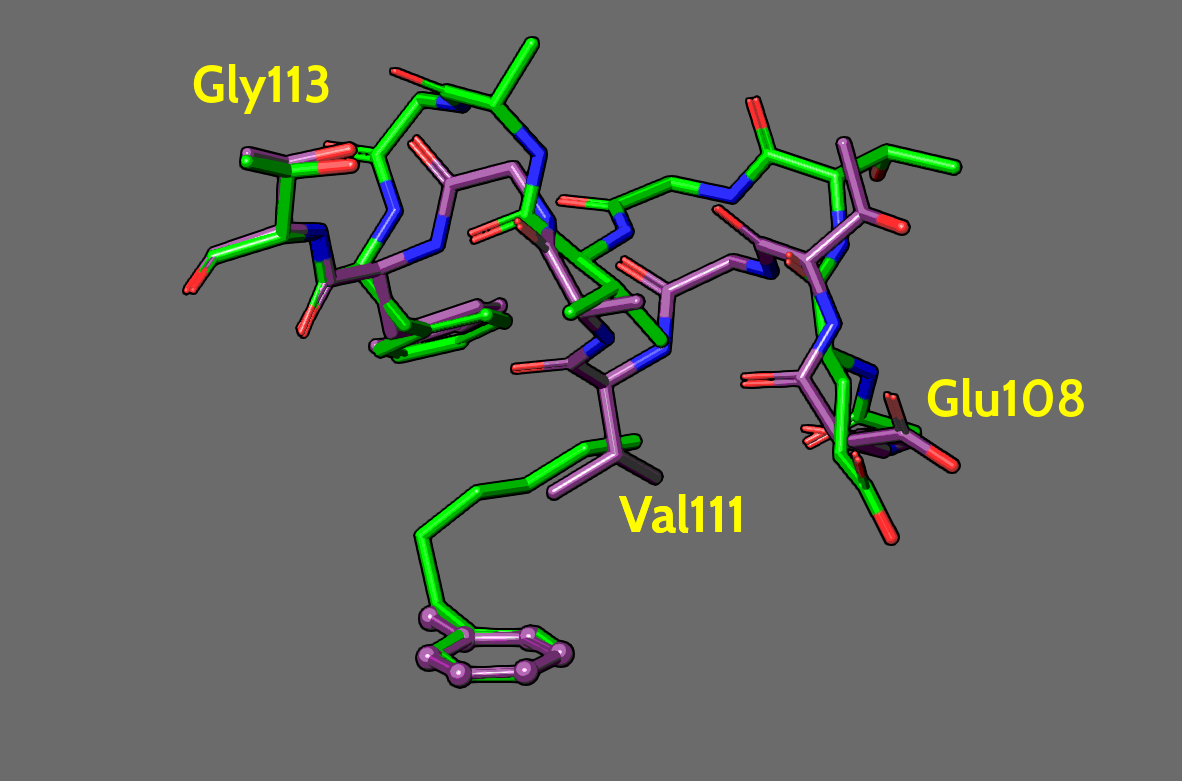
\includegraphics[trim={0cm 3cm 0cm 1cm}, clip, height=0.4\textheight]{Figures/Protein/C2O.png}}
\end{subfigure}\hfill
\centering
\begin{subfigure}{.45\textwidth}
  \centering
   \frame{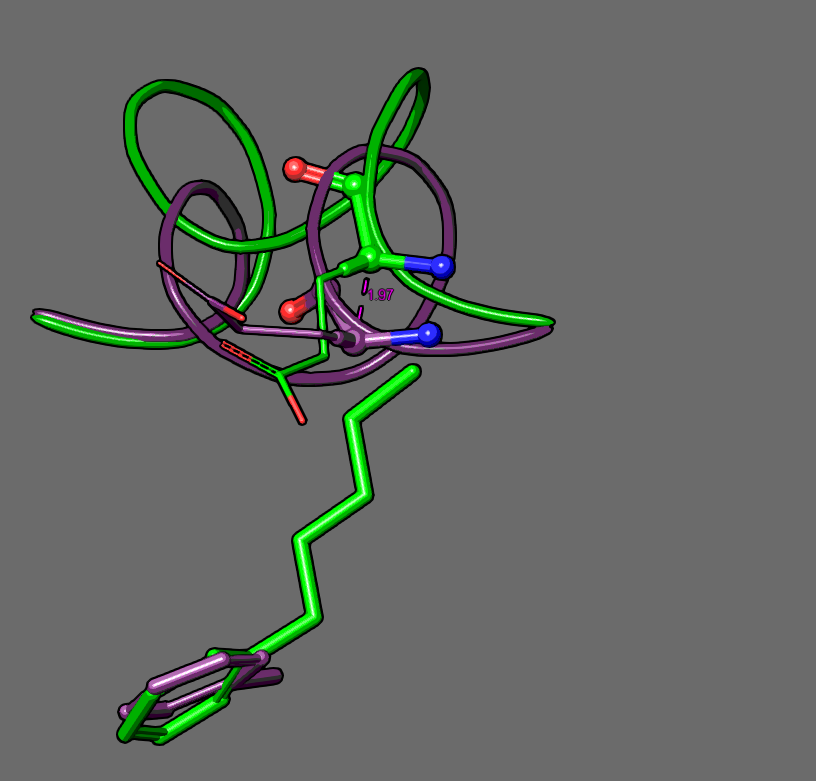
\includegraphics[trim={1cm 0cm 8cm 2cm}, clip, height=0.4\textheight]{Figures/Protein/Glu108-C2O.png}}
   \caption{Residue Glu108}
   \label{fig:Glu108-C2O}
\end{subfigure}\hfill
\begin{subfigure}{.55\textwidth}
   \centering
   \frame{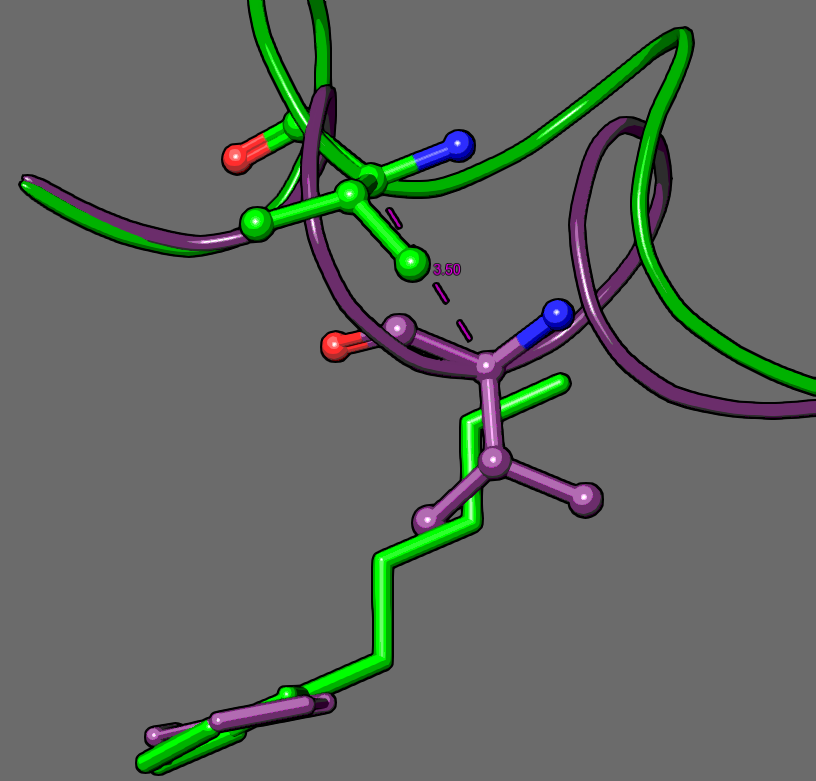
\includegraphics[trim={2cm 0cm 0cm 0cm}, clip, height=0.4\textheight]{Figures/Protein/Val111-C2O.png}}
   \caption{Residue Val111}
   \label{fig:Val111-C2O}
\end{subfigure}\hfill
\caption[T4-L99A REST region]{Fig.~\ref{fig:C2O} highlights the 3 residues selected to be included into the REST region for `pREST' simulations.
Fig.~\ref{fig:Glu108-C2O} and Fig.~\ref{fig:Val111-C2O} illustrates the motion of the $C_{\alpha}$'s during the transition between the protein closed and open states, where the $C_{\alpha}$ in Glu108 undergoes a motion of approximately 2\AA, while in Val11 the $C_{\alpha}$ move approximately 3.5\AA.}
\label{fig:pRESTresidues}
\end{figure}

\subsection{REST region selection}
In this study, by default, only heavy atoms in the ligand were included in the REST region unless specified otherwise.
Further details on the temperature profile and how the REST region is normally selected can be found in previous studies\cite{FEP/REST,FEPplus} in the supporting information.
Simulations that included protein heavy atoms in the REST region are referred to with the `pREST' label, where selection of the particular residues is described as follows.

Based on visual inspection of our molecular dynamics simulations and considering the F-helix spans residues 107-115, we selected residues Glu108, Val111, and Gly113 to include into the REST region (Fig~\ref{fig:C2O}).
Glu108 sits near the start of the helix which appears as a hinge point for the opening and closing of the binding cavity (Fig~\ref{fig:Glu108-C2O}).
Following, Val111 appears in the middle of the helix and was observed to undergo the largest motion during protein conformational changes (Fig~\ref{fig:Val111-C2O}).
Gly113 was included in order to collectively have hot regions approximately at the start, middle and end points of the helix.

\subsection{Simulation details}
Desmond\cite{DESMONDSoftware,DESMONDarticle,DESMONDPaper1,DESMONDPaper2} simulation protocols have been described previously in the supporting information\cite{FEPplus} or can be found in greater detail in the Desmond User Manual\cite{DESMONDManual}.
The relaxation protocol begins with a simulation where solute molecules are restrained to their initial positions while minimizing using a Brownian dynamics NVT integrator for 100ps, followed by 12ps simulations at 10K with a NVT ensemble and then a NPT ensemble using the Langevin method\cite{Langevin}.
Next is a 24ps simulation followed by a final 240ps simulation with solute molecules unrestrained, both are carried at room temperature with a NPT ensemble using Langevin.
Production simulations with the default REST region were ran for the default setting of 5ns.
Initial `pREST' production simulations were also simulated for 5ns and then were carried out to a length of up to 55ns for all closed-open transformations.
For closed-intermediate transformations, we extended `pREST' production simulations up to 25ns, only for cases that were far from convergence with the 5ns simulation time.
Here, we use the final 15ns for closed-open simulations and the final 10ns for closed-intermediate to calculate our final free energies, discarding the initial time as additional equilibration time.
FEP/REST simulations were run on four GeForce GTX Titan Black GPUs using the Desmond/GPU engine with the recently developed OPLS3\cite{OPLS3} forcefield parameters.

\subsection{Calculation of free energies and measurement of inconsistency}
Throughout this study, we measure the inconsistency ($\Delta\Delta G_{\boldsymbol{\varepsilon_n}}$) between the final calculated free energies between simulations that start from the protein closed state ($\Delta\Delta G_{\mathbf{C_n}}$) versus the protein open state ($\Delta\Delta G_{\mathbf{O_n}}$) by simply taking the difference.
\begin{equation}
  \mathbf{\Delta\Delta G_{\boldsymbol{\varepsilon_n}}}  = \left |  \Delta\Delta G_{\mathbf{C_n}  } - \Delta\Delta G_{\mathbf{O_n} }\right |
  \label{eqn:diffG}
\end{equation}
Then we compute the overall inconsistency---referred to as the 'Root-Mean-Square-Inconsistency' (RMSI)---for each set of alchemical transformations.
The RMSI is calculated by using the differences ($\Delta\Delta G_{\boldsymbol{\varepsilon_n}}$) obtained from the comparisons between protein open and closed simulations.
\begin{equation}
\mathbf{RMSI} = \sqrt{   \frac{ \sum_{n} (\Delta\Delta G\varepsilon_{n} )^2  } {n}}
  \label{eqn:RMSI}
\end{equation}
Similarly, we compute the 'Root-Mean-Square-Error'(RMSE) when comparing with experimental free energies for both simulations starting from the protein closed and open state.
\begin{equation}
\mathbf{RMSE^{O}} = \sqrt{   \frac{ \sum_{n} (\Delta\Delta G_{\mathbf{O_n}} - \Delta\Delta G_{\mathbf{exp_n}} )^2  } {n}}
\mathbf{RMSE^{C}} = \sqrt{   \frac{ \sum_{n} (\Delta\Delta G_{\mathbf{C_n}} - \Delta\Delta G_{\mathbf{exp_n}} )^2  } {n}}
  \label{eqn:RMSE}
\end{equation}
Calculated free energies were determined using the Bennett acceptance ratio\cite{BAR} (BAR) with error estimations using both bootstrapping and BAR analytical error prediction\cite{BARerror}.
Hysteresis around closed thermodynamic cycles and best estimates of the free energies with their errors were calculated using the cycle closure algorithm discussed in a previous publication\cite{FEP/REST}.

\subsection{Determining the protein conformation state using RMSD}
In this study, we determine the state of the protein by computing the 'Root-Mean-Square-Deviation' (RMSD) of the protein backbone atoms spanning the F-helix relative to their positions found in the closed (PDB:4W53), intermediate (PDB:4W57), and open (PDB:4W59) crystal structures (Fig~\ref{fig:T4-L99A_tube}).
The set of RMSDs---that is, the RMSD relative to the closed, intermediate, and open states---is computed at each frame over the course of the entire simulation.
Then, we use the protein conformational state with the lowest RMSD to correspondingly color each time point in our analyses of `RMSD/time' and `Color maps'.
Again, we use purple to denote the protein closed state, cyan for the intermediate state, and green for the open state.
Here, we use VMD \cite{VMDpaper,VMDalignment} to align and compute the RMSD of our Desmond trajectories relative to crystal structures.
Further details on the procedure and the scripts used for these analyses are provided in the supplementary info.

For the `RMSD/time' analysis, see Figure~\ref{fig:o_opls3_1/RMSD-replica11}) for reference.
Here, we plot the RMSD to the closed helix, represented by the black line, where each time point is colored according to the lowest RMSD state.
We apply the RMSD/time analysis only to the simulation corresponding to the end state ligand of interest ($\lambda_{11}$).
By tracking the RMSD relative to the closed helix, we can monitor if the protein opens (by high RMSD with green points) or closes (by low RMSD with purple points).
Additionally, we gain some insight on the time required to capture the opening or closing of the binding cavity.

It is important to note that by restraining our analysis to only the end-state replica, we limit our ability to completely view the effects of coordinate swapping during replica exchanges.
We address this limitation by analyzing all replicas in what we call `Color maps', see Figure~\ref{fig:c_opls3_rest1_1/colormap} for an example.
Essentially, our 'Color map' analysis is the same as our 'RMSD/time' plots but without the RMSD line plot.
In other words, we color time points according to the protein state of lowest RMSD and do this for all replicas but do not track the RMSD relative to the closed state.
Through a collective view of all replicas, we gain a better perspective of the overall protein conformational sampling and the states they occupy over each replica's separate trajectories.
Using color maps, it becomes visually easy to see if intermediate---higher temperature---lambda windows are able to sample, say the open state, and if this leads to an enhancement in sampling at the end states via replica exchange.

\section{Results}

\subsection{Calculated free energies depend strongly on starting protein conformation}
Using the default FEP/REST methodology\cite{FEP/REST}, we find calculated free energies significantly depend on the protein starting conformation, especially for large perturbations (i.e. opening the cavity from the closed state).
To illustrate this, we begin our molecular dynamics simulations both from the protein closed and open conformations then perform alchemical transformations to ligands that occupy another protein conformational state.
For example, in the alchemical transformation of benzene to hexylbenzene---starting from the protein closed state---we expect to see opening of the binding cavity when the ligand is in the fully interacting hexylbenzene state.
In this study, we demonstrate using the default FEP protocol settings of a 5ns simulation time and REST region selection does not generate adequate sampling of the motion in the F-helix and does not eliminate the dependence on the initial protein state.

\paragraph{Closed-Open Ligand Transformations}

\begin{figure}[H]
\begin{subfigure}{\textwidth}
   \centering
    \caption{Protein closed simulation}
   \label{fig:c_opls3_1/RMSD-replica11}
   \frame{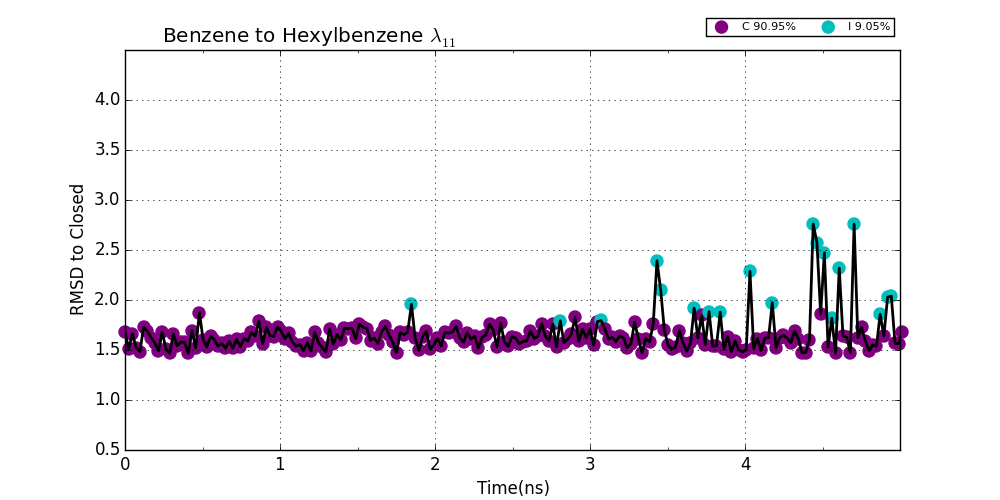
\includegraphics[trim={1.5cm 0 2cm 0.25cm}, clip, width=\linewidth, height=0.3\textheight]{Figures/RMSD-time/benzene-nhexylbenzene_C_default_rep11.png}}
\end{subfigure}
\centering
\begin{subfigure}{\textwidth}
  \centering
  \frame{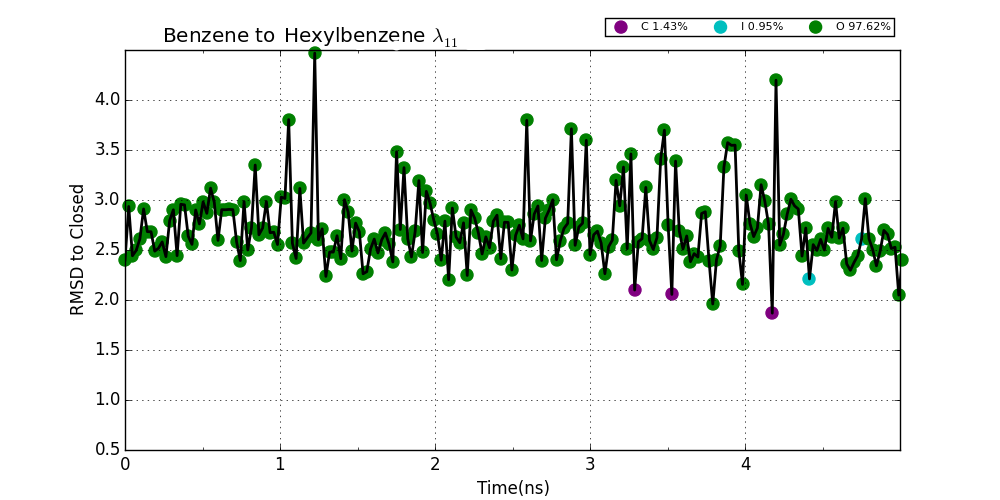
\includegraphics[trim={1.5cm 0 2cm 0.25cm}, clip, width=\linewidth, height=0.3\textheight]{Figures/RMSD-time/benzene-nhexylbenzene_O_default_rep11.png}}
  \caption{Protein open simulation}
  \label{fig:o_opls3_1/RMSD-replica11}
\end{subfigure}%
\caption[RMSD of Hexylbenzene bound to protein closed/open]{Plotted is the RMSD(\AA) relative to the closed helix conformation (black line), where each time point is colored according to the protein state of lowest RMSD to the trajectory.
Here, using the default protocol in the transformation of benzene to hexylbenzene, RMSD/time plots correspond to the final end state of hexylbenzene ($\lambda_{11}$).
Fig.~\ref{fig:c_opls3_1/RMSD-replica11} corresponds to the simulation that began from the protein closed state and Fig.~\ref{fig:o_opls3_1/RMSD-replica11} is from the simulation started from the protein open state.
The legends indicate the percentage of sampling of each protein conformational state from the trajectory.}
\label{fig:benzene_to_n-hexyl}
\end{figure}

An examination of the largest alchemical transformation, benzene to hexylbenzene, clearly highlights the sampling challenges faced when using the default FEP/REST protocol.
From experimental data of ligand occupancies (Table~\ref{tbl:expdata}), we expect in our simulations of hexylbenzene to see the protein primarily in the open state over the closed state.
Instead, we find the protein remains trapped in its initial conformational state whether we start from closed (Fig~\ref{fig:c_opls3_1/RMSD-replica11}) or open (Fig~\ref{fig:o_opls3_1/RMSD-replica11}) over the course of the 5ns simulation.
From the protein closed simulation, the protein only briefly samples the intermediate state around 3ns but never enters the open conformation.
As the protein tries to accommodate hexylbenzene and enter its preferred open state, protein-ligand strain results, yielding a positive value for $\Delta\Delta G_{calc}$(+4.13 kcal/mol).
On the other hand, in the protein open simulations, the protein already begins in its preferred state for hexylbenzene and stays only in this open state.
As expected, the $\Delta\Delta G_{calc}$ is negative(-0.61 kcal/mol) as there is no occurrence of large protein-ligand strain in order to open the cavity.
By remaining trapped in the initial state, we under-sample the open state if we begin from the closed state or over-sample it if we begin from the open state.
Ultimately, we arrive at two very different relative free energies values, where the inconsistency is as large as +4.74 kcal/mol for the same transformation of benzene to hexylbenzene.

In the overall set, we similarly observe protein closed simulations to yield positive free energies and negative for protein open simulations.
In turn, we find the overall inconsistency to be very high with a RMSI of +4 kcal/mol (Fig~\ref{fig:C2O_xyplot}, Table~S\ref{tbl:C-O}).
Clearly, despite the use of implemented default FEP/REST protocol, we are unable to get sufficient sampling in the protein within the standard 5ns time frame.
This is perhaps unsurprising since in the default calculation, only the perturbed ligand R-group is added to the enhanced sampling region.
Instead, we encounter sampling problems as the protein remains in its initial conformational state throughout the simulation.
As a result, our calculated free energies exhibit high dependence on the initial protein configuration which is reflected by the large RMSI.

\paragraph{Closed-Intermediate Ligand Transformations}
In the case of closed-intermediate alchemical transformations, we find that the calculated free energies still have some (albeit much smaller) dependence on the initial protein conformation, using the default protocol.
For this set of alchemical transformations, we find the RMSI to be +0.60 kcal/mol (Fig~\ref{fig:C2I_xyplot}, Table~S\ref{tbl:C-I}).
Considering this set involves a smaller protein conformational change and smaller perturbations to the ligand, it is unsurprising to find the RMSI to be much smaller than our closed-open transformation set.

Although, the collective RMSI for closed-intermediate transformations falls in the acceptable range of less than 1 kcal/mol, we can still see a dependence on the initial protein configuration by viewing transformations involving butylbenzene.
For these cases in particular, we observe the same pattern of protein closed simulations yielding positive free energies and negative for protein open simulations.
We do not see this pattern for transformations with sec-butylbenzene as it does not partially occupy the open state, unlike butylbenzene (Table~\ref{tbl:expdata}).
Through this observation, we demonstrate further that the default protocol does not completely eliminate the free energy dependence on the protein starting conformation, even for smaller perturbations.
Although, the level of discrepancy (0.6 kcal/mol) is quite small for this set.

\paragraph{Experimental Ligand Transformations}

\begin{figure}[!ht]
\begin{subfigure}{\textwidth}
   \centering
    \caption{Protein closed simulation}
   \label{fig:c_exp_opls3_11/RMSD-replica11}
   \frame{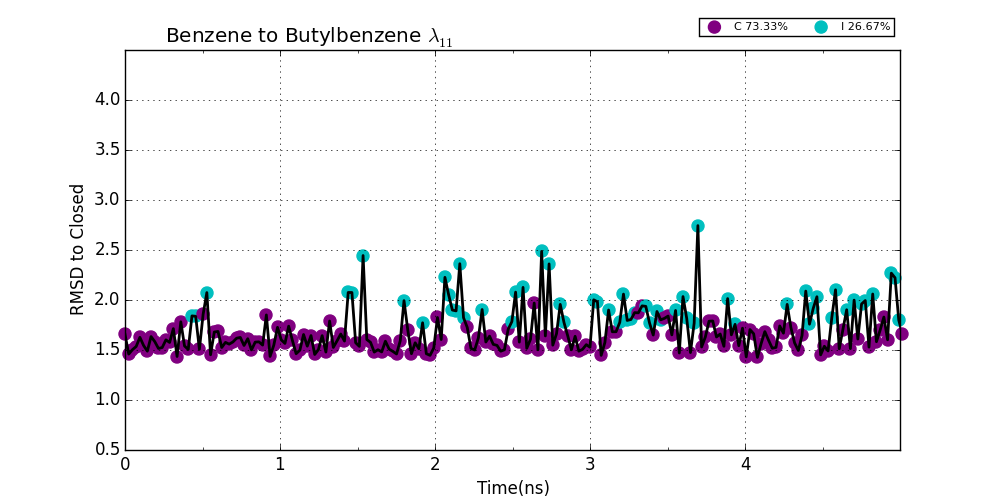
\includegraphics[trim={1.5cm 0 2cm 0.25cm}, clip, width=\linewidth, height=0.3\textheight]{Figures/RMSD-time/benzene-nbutylbenzene_C_default_rep11.png}}
\end{subfigure}
\centering
\begin{subfigure}{\textwidth}
  \centering
   \frame{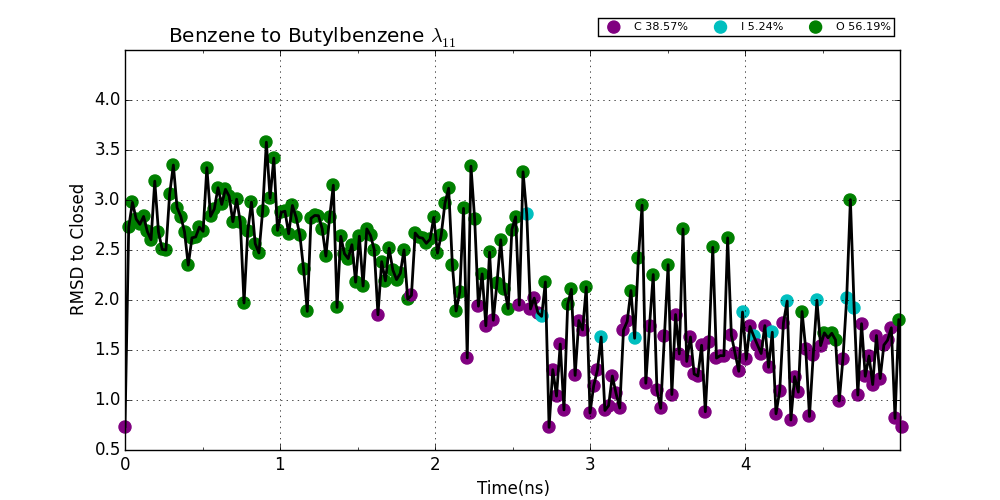
\includegraphics[trim={1.5cm 0 2cm 0.25cm}, clip, width=\linewidth, height=0.3\textheight]{Figures/RMSD-time/benzene-nbutylbenzene_O_default_rep11.png}}
   \caption{Protein open simulation}
   \label{fig:o_exp_opls3_24/RMSD-replica11}
\end{subfigure}%
\caption[RMSD of Butylbenze bound to protein closed/open]{RMSD/time plots correspond to the final end state of butylbenzene ($\lambda_{11}$) while using the default protocol for transformation of benzene to butylbenzene.
Fig.~\ref{fig:c_exp_opls3_11/RMSD-replica11} and Fig.~\ref{fig:o_exp_opls3_24/RMSD-replica11}
correspond to simulations that were started from the protein closed or open state, respectively.
The legends indicate the percentage of sampling of each protein conformational state from the trajectory.
}
\label{fig:benzene_to_n-butyl}
\end{figure}

Now, when we compare $\Delta\Delta G_{calc}$ against $\Delta\Delta G_{exp}$, we find that simulations starting from the protein closed conformation are further from converging to $\Delta\Delta G_{exp}$ than when starting from the protein open conformation.
Here, we calculate the RMS-'Error' with experiment and find the RMSE for protein closed simulations to be +1.0 kcal/mol and +0.58 kcal/mol with protein open (Fig~\ref{fig:exp_xyplot},Table~S\ref{tbl:exp_set}).
Our total RMSI falls within our acceptable range at 0.68 kcal/mol.
However, the fact that protein open simulations are much closer to $\Delta\Delta G_{exp}$, once again does demonstrate our calculated free energies depend on the initial protein state.
Unsurprisingly, the relatively larger RMSE seen for protein closed simulations primarily comes from transformations involving butylbenzene.
Evidently, we find the simulations involving butylbenzene remain trapped in their respective starting conformations, resulting in inadequate sampling in the protein closed simulations (Fig.~\ref{fig:c_exp_opls3_11/RMSD-replica11}) versus the protein open simulations (Fig.~\ref{fig:o_exp_opls3_24/RMSD-replica11}).
Despite performing much smaller alchemical transformations, this shows we still encounter some sampling problems that result in $\Delta\Delta G_{calc}$ that depend on the initial protein conformation, evident when comparing to $\Delta\Delta G_{exp}$.

\subsection{Including protein residues into the REST region (pREST) improves sampling}

\begin{figure}[H]
\begin{subfigure}{.5\textwidth}
  \centering
  \caption{Default}
   \label{fig:c_opls3_1/colormap}
   \frame{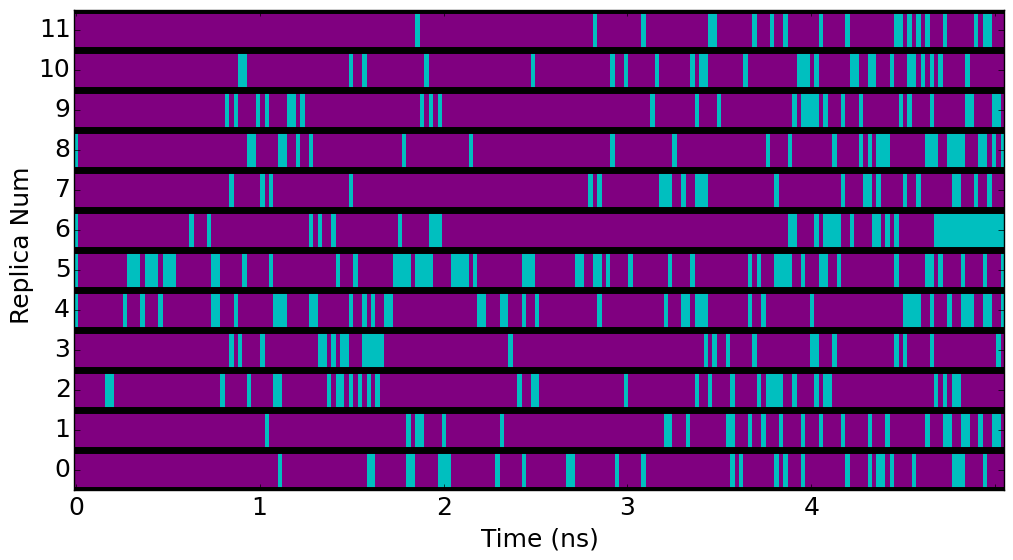
\includegraphics[width=\linewidth, height=0.3\textheight]{Figures/Colormap/benzene-nhexylbenzene_C_default.png}}
\end{subfigure}\hfill
\begin{subfigure}{.5\textwidth}
   \centering
    \caption{pREST}
   \label{fig:c_opls3_rest1_1/colormap}
   \frame{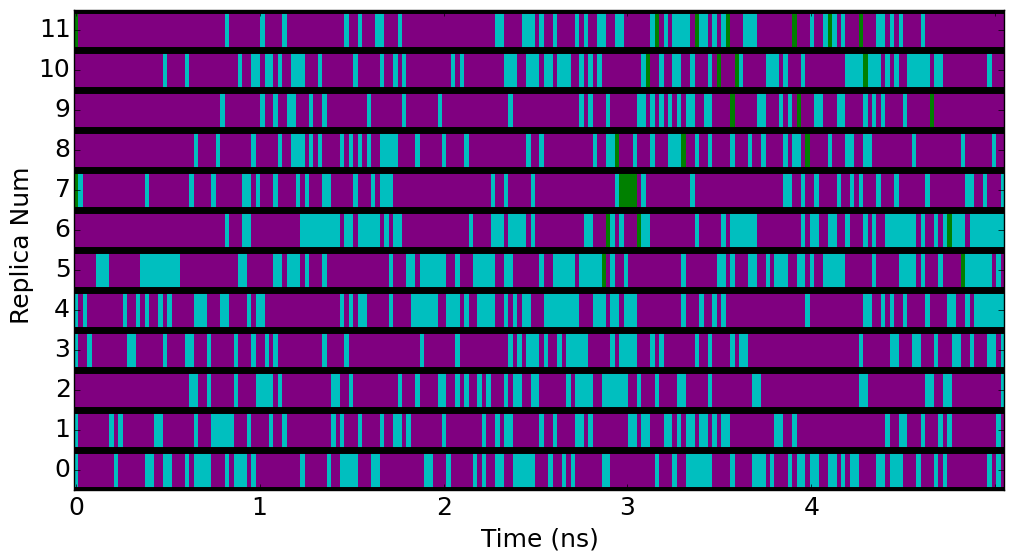
\includegraphics[width=\linewidth, height=0.3\textheight]{Figures/Colormap/benzene-nhexylbenzene_C_pREST.png}}

\end{subfigure}\hfill
\centering
\begin{subfigure}{\textwidth}
   \centering
   \frame{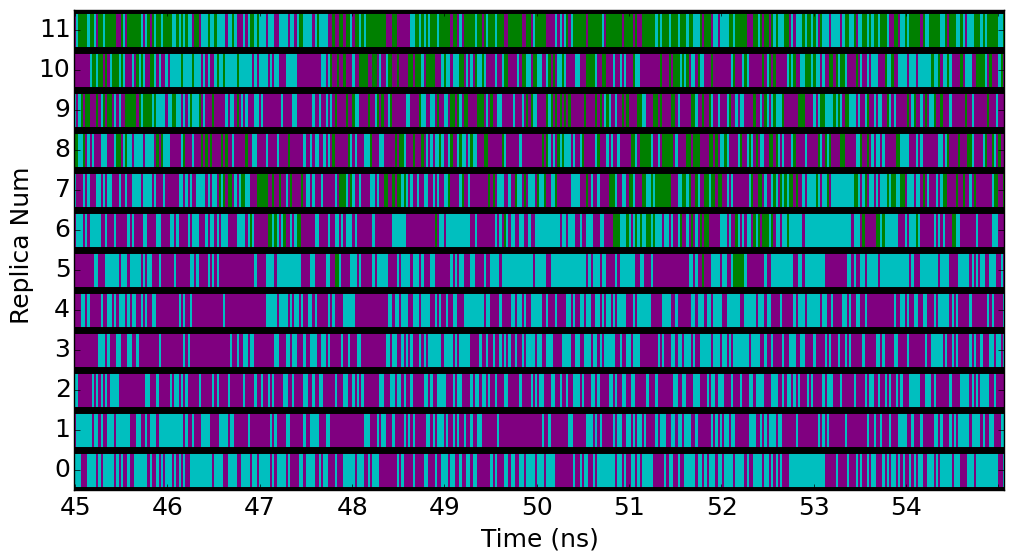
\includegraphics[clip, width=\linewidth, height=0.3\textheight]{Figures/Colormap/benzene-nhexylbenzene_C_pRESText.png}}
   \caption{pREST extended}
   \label{fig:c_opls3_rest1_1/cmap-45-55ns}
\end{subfigure}\hfill
\caption[Sampling of protein conformational state]{Color maps of simulations starting from the protein closed state for the benzene to hexylbenzene alchemical transformation.
Lines at every frame are colored accordingly to the protein state of lowest RMSD (purple-closed, cyan-intermediate, green-open).
Fig.~\ref{fig:c_opls3_1/colormap} corresponds to simulations using the default protocol. Fig.~\ref{fig:c_opls3_rest1_1/colormap} represents simulations using the modified REST region protocol (pREST). Fig.~\ref{fig:c_opls3_rest1_1/cmap-45-55ns} illustrates the enhancement in protein conformational sampling through extending the pREST simulation time up to 55ns.
}
\label{fig:benzene_to_n-hexyl_colormap}
\end{figure}

Primarily, we encounter major sampling problems when we begin our simulations from the protein closed state and attempt a mutation which should result in the binding cavity opening.
In order to facilitate protein motion, thereby enhancing protein sampling, we included 3 key residues spanning the F-helix region into the REST region, which we will denote simulations using this with `pREST' (Fig~\ref{fig:C2O}).
By expanding the REST region, we are able to drive the F-helix out its initial state trap by locally heating up key regions and thereby reduce our sampling problem.

To demonstrate the REST improvement over the default protocol, we return to the case of benzene to hexylbenzene.
Here, we show the facilitation of the helix motion by first referring to Figure~\ref{fig:c_opls3_1/RMSD-replica11} which shows that there is no sampling of the open state for the default protocol.
Now with pREST, we see a few open state points around 3ns and even a single open point before closing again after our initial step (Fig~\ref{fig:c_opls3_rest1_1/RMSD-replica11}).
Alternatively, we can further illustrate the enhancement of protein sampling by viewing all replicas collectively, using the color maps.
In reference to Figure~\ref{fig:c_opls3_1/colormap} and Figure~\ref{fig:c_opls3_rest1_1/colormap}, we illustrate that there is far less sampling of the intermediate or open protein states in default simulations versus the pREST simulations.

Collectively, we find only some minor improvements in the RMSI for all our closed-open and closed-intermediate transformations while using pREST.
For closed-open transformations (Table~S\ref{tbl:C-O_pREST}), the RMSI reduces to +2.82 kcal/mol (previously +4 kcal/mol).
On the other hand, for closed-intermediate, the RMSI raises slightly to +0.79 kcal/mol (previously +0.60 kcal/mol), which may be due to statistical noise (Table~S\ref{tbl:C-I_pREST}).
Generally, simulations starting from the closed state had $\Delta\Delta G_{calc}$ values that moved towards favorability (i.e. more negative $\Delta\Delta G_{calc}$), while for protein open simulations $\Delta\Delta G_{calc}$ values tended towards unfavorability (i.e. more positive $\Delta\Delta G_{calc}$).
This is indicative of the fact that pREST is indeed improving sampling, but it is evident that our $\Delta\Delta G_{calc}$ are still far from convergence, given the RMSI is still large, especially for closed/open transformations.

\subsection{Long simulations enhances protein conformational sampling from more exchanges}

\begin{figure}[H]
\centering
\begin{subfigure}{.5\textwidth}
  \centering
    \caption{Closed-Open: Default}
   \label{fig:C2O_xyplot}
   \frame{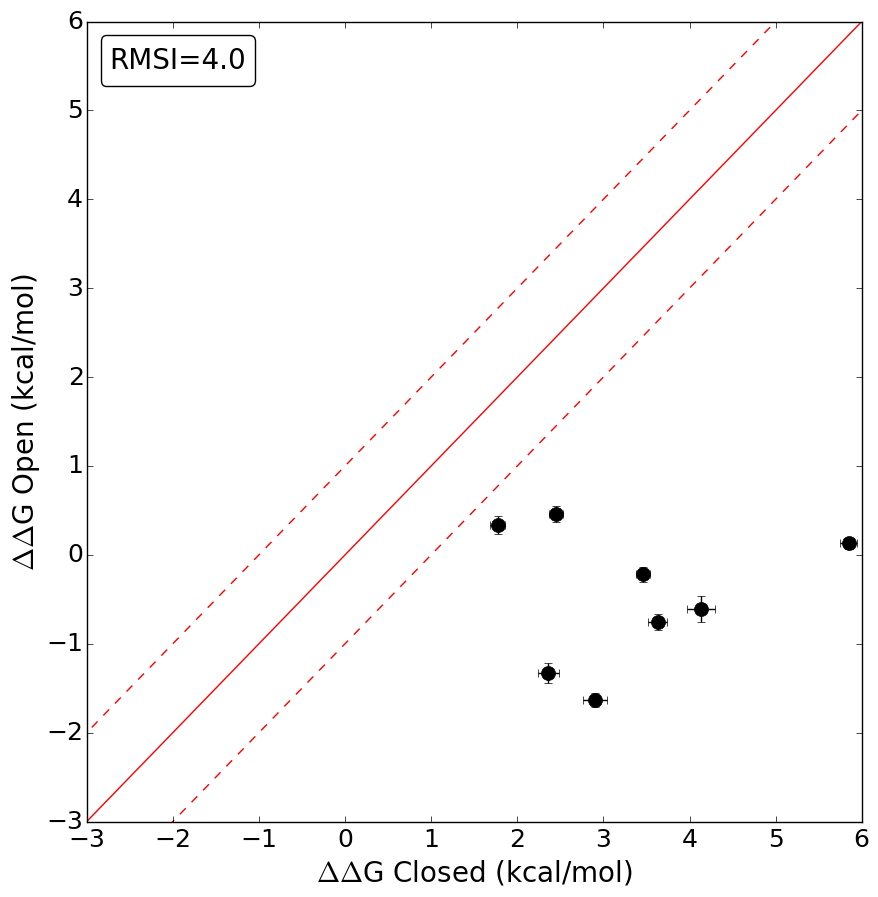
\includegraphics[width=\linewidth, height=0.3\textheight]{Figures/XYplot/C2O_xyplot.png}}
\end{subfigure}\hfill
\begin{subfigure}{.5\textwidth}
   \centering
  \caption{Closed-Open: pREST}
   \label{fig:C2O_xyplot_pREST}
   \frame{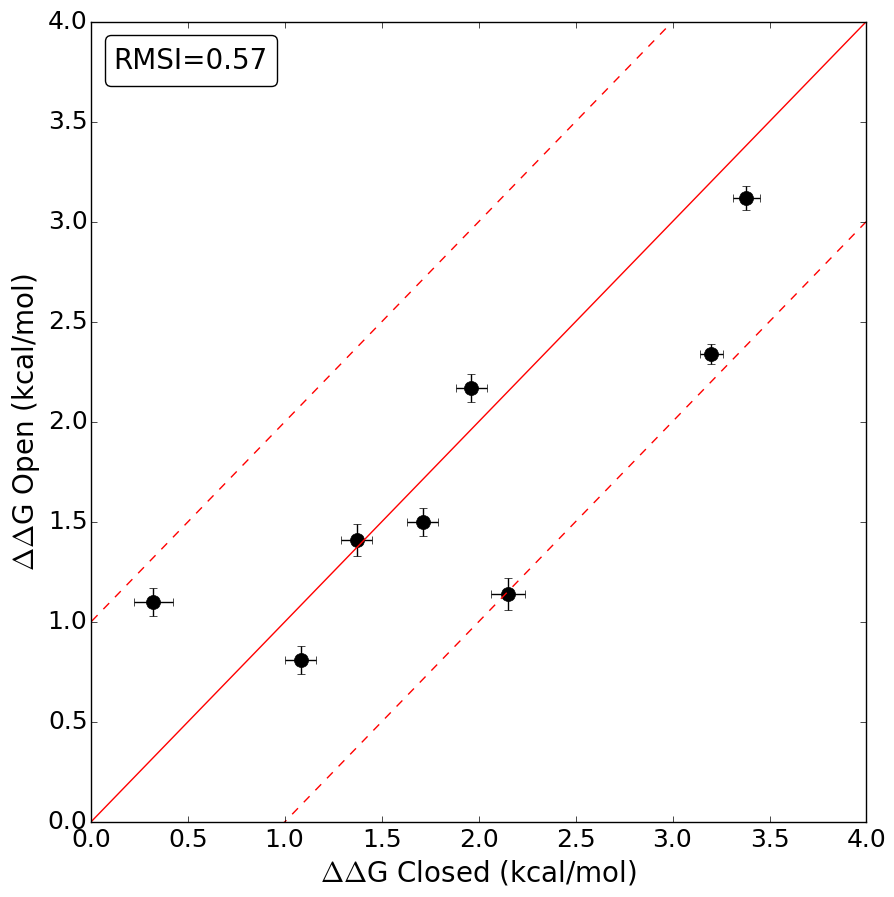
\includegraphics[width=\linewidth, height=0.3\textheight]{Figures/XYplot/C2O_pREST_xyplot.png}}
\end{subfigure}\hfill
\centering
\begin{subfigure}{.5\textwidth}
  \centering
   \frame{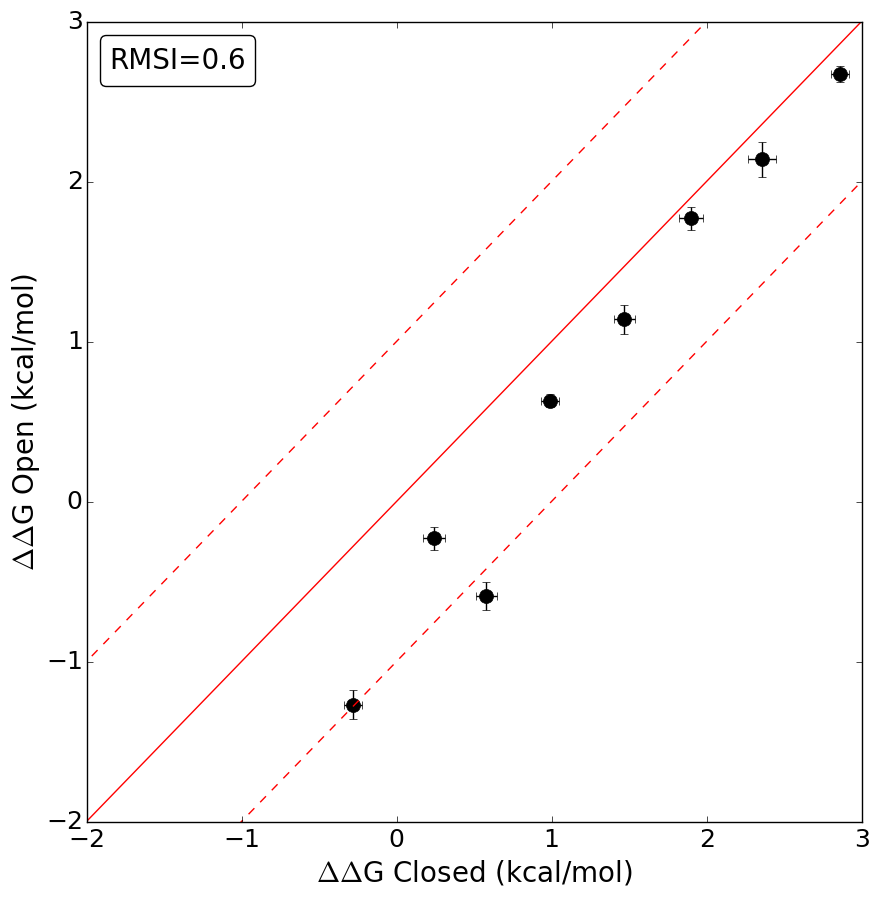
\includegraphics[width=\linewidth, height=0.3\textheight]{Figures/XYplot/C2I_xyplot.png}}
   \caption{Closed-Intermediate: Default}
   \label{fig:C2I_xyplot}
\end{subfigure}\hfill
\begin{subfigure}{.5\textwidth}
   \centering
   \frame{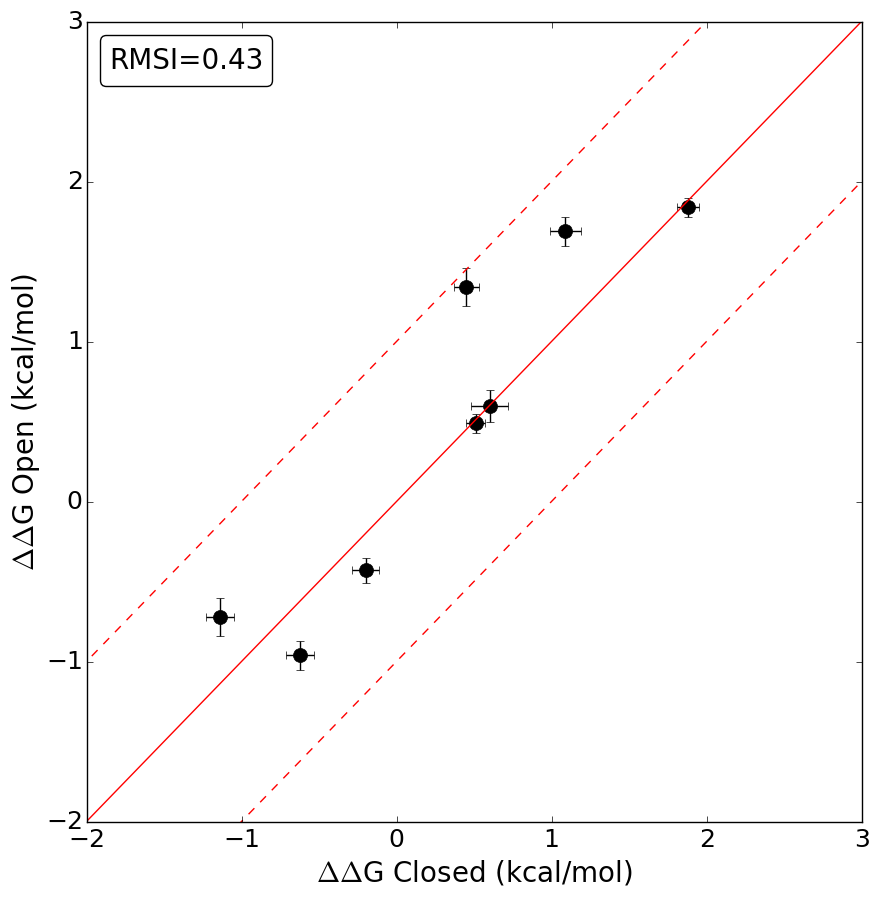
\includegraphics[width=\linewidth, height=0.3\textheight]{Figures/XYplot/C2I_pREST_xyplot.png}}
   \caption{Closed-Intermediate: pREST}
   \label{fig:C2I_xyplot_pREST}
\end{subfigure}\hfill
\caption[$\Delta\Delta G_{calc}$ from MD simulations]{$\Delta\Delta G_{calc}$ from MD simulations beginning from the protein closed versus open state.
Fig.~\ref{fig:C2O_xyplot} plots relative free energies obtained using the default protocol from the `closed-open' alchemical transformations set, yielding a RMSI of 4.0 kcal/mol.
Fig.~\ref{fig:C2O_xyplot_pREST} are the final computed free energies with simulations carried out to 55ns using pREST, giving RMSI of 0.57 kcal/mol.
Fig.~\ref{fig:C2I_xyplot} plots relative free energies from the `closed-intermediate' set using the default protocol which gives an RMSI of 0.6 kcal/mol.
Fig.~\ref{fig:C2I_xyplot_pREST} are free energies with simulations carried out up to 25ns using pREST, giving RMSI of 0.43 kcal/mol.
Numerical data for each plot can be found in Tables~S\ref{tbl:C-I}, S\ref{tbl:C-I_pRESText}, \ref{tbl:C-O}, and SS\ref{tbl:C-O_pREST-40-55ns}.
}
\label{fig:conf-xyplots}
\end{figure}

Although we see improvements in sampling with pREST, the standard implemented time frame of 5ns clearly is not long enough to gain adequate sampling, particularly if we start from the protein closed state.
By running longer, we allow our simulations to perform more exchanges across replicas and thereby allow for better sampling of all conformational states at the relevant end state replicas.

\begin{figure}[H]
\begin{subfigure}{\textwidth}
   \centering
    \caption{Protein closed simulation, pREST}
   \label{fig:c_opls3_rest1_1/RMSD-replica11}
   \frame{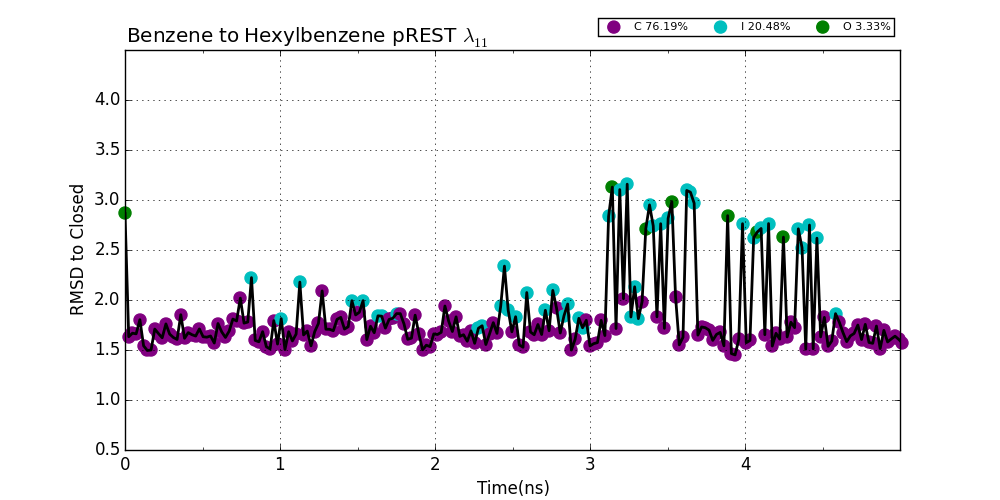
\includegraphics[trim={1.5cm 0 2cm 0.25cm}, clip, width=\linewidth, height=0.3\textheight]{Figures/RMSD-time/benzene-nhexylbenzene_C_pREST_rep11.png}}
\end{subfigure}
\centering
\begin{subfigure}{\textwidth}
  \centering
   \frame{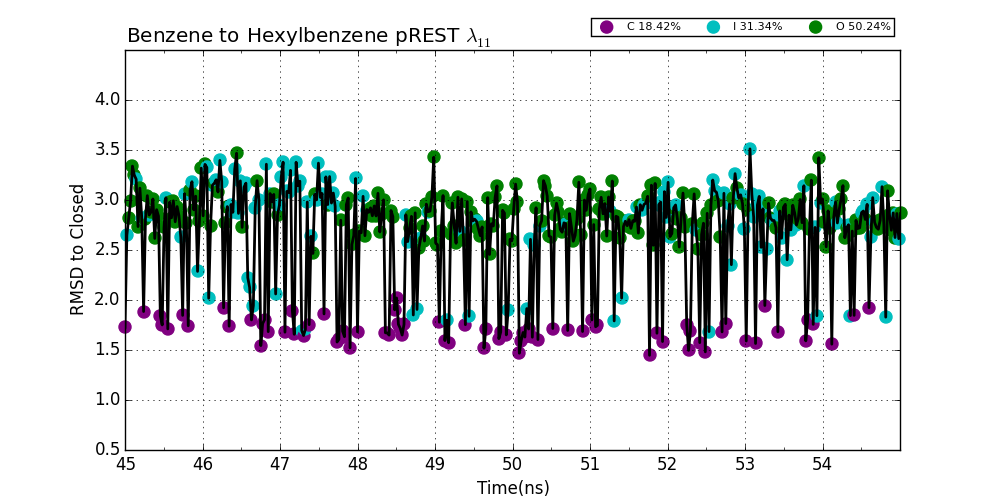
\includegraphics[trim={1.5cm 0 2cm 0.25cm}, clip, width=\linewidth, height=0.3\textheight]{Figures/RMSD-time/benzene-nhexylbenzene_C_pRESText_rep11.png}}
   \caption{Protein closed simulation, pREST extended}
   \label{fig:c_opls3_rest1_1/45-55ns/RMSD-replica11}
\end{subfigure}%
\caption[RMSD of hexylbenzene bound to protein closed/open using pREST]{Using the modified REST region (pREST) in the transformation of benzene to hexylbenzene, we plot the RMSD/time corresponding to the hexylbenzene state ($\lambda_{11}$) with the simulation starting from protein closed for the first 5ns (Fig.~\ref{fig:c_opls3_rest1_1/RMSD-replica11}) and the final 10ns from an extended run up to 55ns (Fig.~\ref{fig:c_opls3_rest1_1/45-55ns/RMSD-replica11}).}
\label{fig:benzene_to_n-hexyl_pREST}
\end{figure}

Returning to our most extreme transformation, benzene to hexylbenzene, we have shown pREST alone does not facilitate adequate sampling of the open state (Fig~\ref{fig:c_opls3_rest1_1/RMSD-replica11}).
Now, when we run much longer we see far more sampling of the open protein conformational state in the final 10ns window (Fig~\ref{fig:c_opls3_rest1_1/45-55ns/RMSD-replica11}).
Note that, for closed-open transformations we use the final 15ns to compute the final free energies.
We only show the final 10ns in our RMSD/time analysis to avoid overcrowding data points.
In viewing all the replicas (Fig~\ref{fig:c_opls3_rest1_1/cmap-45-55ns}), we illustrate the dramatic increase in protein conformational sampling in stark contrast to our previous 5ns simulations (Fig~\ref{fig:c_opls3_rest1_1/colormap}).
An additional analysis comparing the protein-ligand contacts between the default and pREST protocol can be found in the Supporting Information (Fig. S1).

By simulating longer with pREST we dramatically increase our sampling of the intermediate and open protein states and almost entirely eliminate the dependence on the initial protein conformational state.
For the set of closed-open transformations the RMSI dramatically falls to +0.57 kcal/mol (Fig.~\ref{fig:C2O_xyplot_pREST},Table ~S\ref{tbl:C-O_pREST-40-55ns}) and a RMSI of +0.43 kcal/mol for the closed-intermediate (Fig.~\ref{fig:C2I_xyplot_pREST},Table ~S\ref{tbl:C-I_pRESText}).
Similarly, for experimental ligand transformations, our RMSE for protein closed simulations falls to +0.54 kcal/mol and the RMSI reduces to 0.31 kcal/mol (Fig.~\ref{fig:exp_xyplot_pREST},Table~S\ref{tbl:exp_pREST_set}).
Now, all our inconsistencies in the final calculated free energies and error from experiment fall within a much more reasonable range of less than +1 kcal/mol.

\begin{figure}[H]
\centering
\begin{subfigure}{.5\textwidth}
  \centering
     \caption{Default}
   \label{fig:exp_xyplot}
   \frame{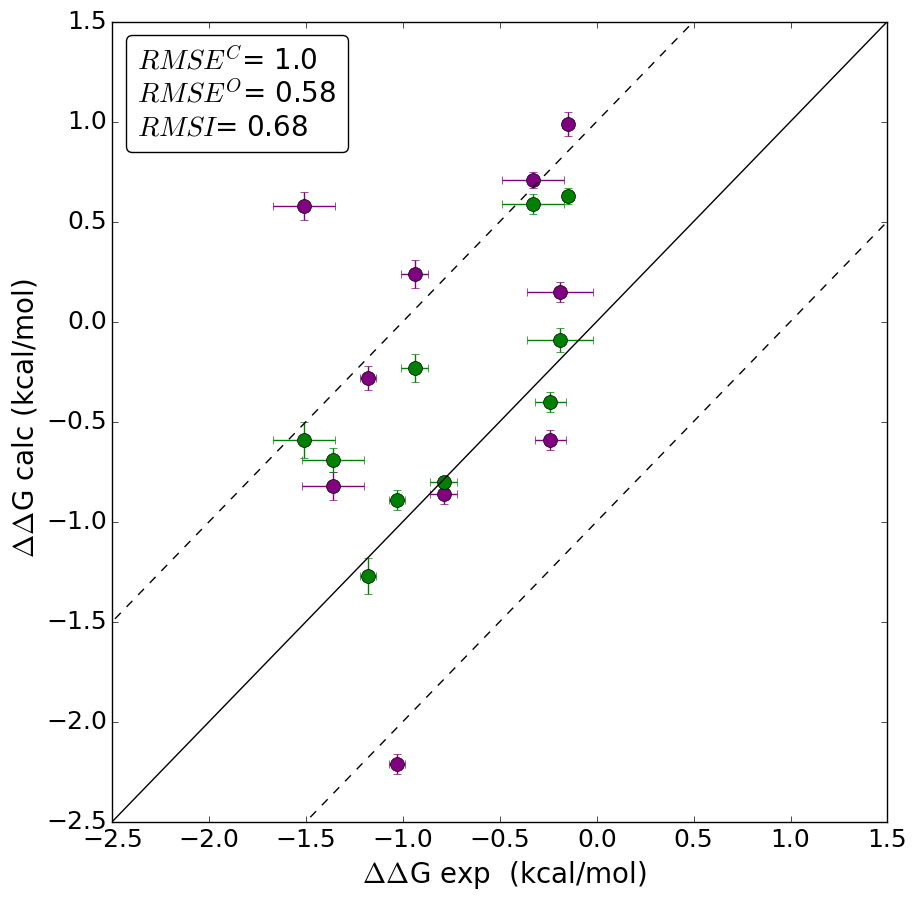
\includegraphics[width=\linewidth, height=0.3\textheight]{Figures/XYplot/exp_xyplot.png}}
\end{subfigure}\hfill
\begin{subfigure}{.5\textwidth}
   \centering
      \caption{pREST}
   \label{fig:exp_xyplot_pREST}
   \frame{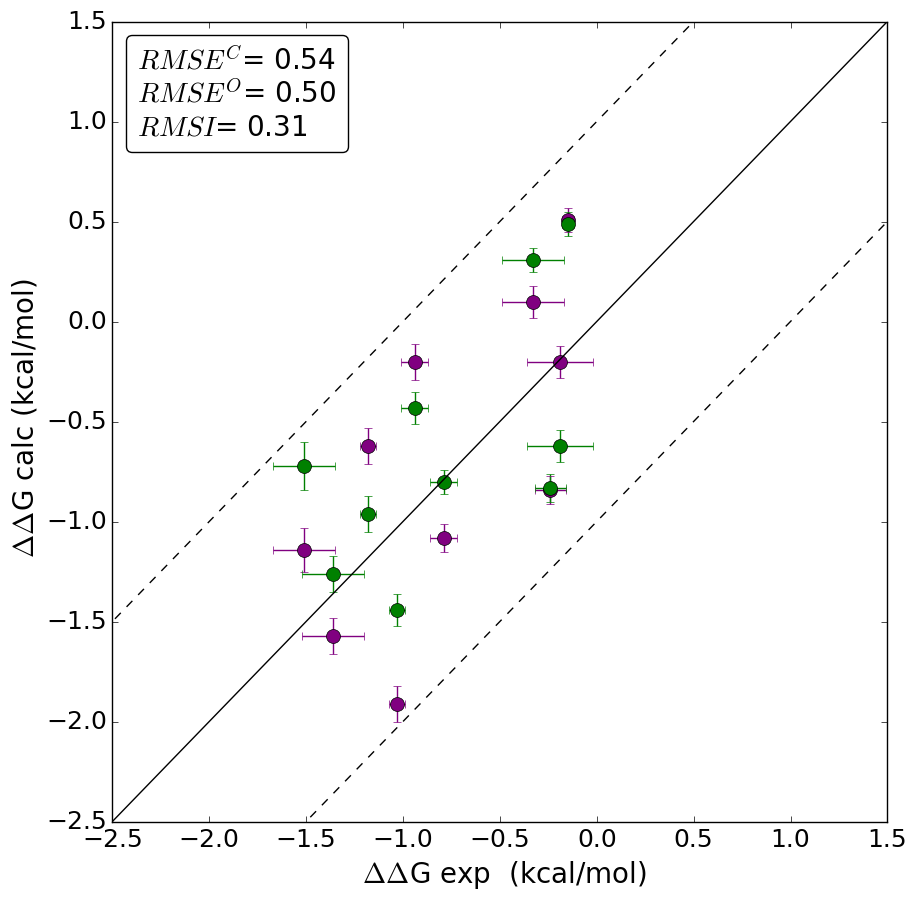
\includegraphics[width=\linewidth, height=0.3\textheight]{Figures/XYplot/exp_pREST_xyplot.png}}
\end{subfigure}\hfill
\caption[$\Delta\Delta G_{calc}$ vs $\Delta\Delta G_{exp}$]{$\Delta\Delta G_{calc}$ from MD simulations beginning from the protein closed (purple) and open (green) state compared against $\Delta\Delta G_{exp}$.
Fig.~\ref{fig:exp_xyplot} plots free energies obtained using the default protocol which gives a 1.0 kcal/mol and 0.58 kcal/mol RMSE for protein closed and open simulations, respectively.
Total RMSI using the default protocol is 0.68 kcal/mol.
Fig.~\ref{fig:exp_xyplot_pREST} plots the final free energies after applying pREST, yielding an RMSE of 0.54 for protein closed and 0.50 kcal/mol for protein closed simulations.
Total RMSI using the pREST protocol is 0.31 kcal/mol.
Numerical data for each plot can be found in Tables~S\ref{tbl:exp_set} and S\ref{tbl:exp_pREST_set}.
}
\label{fig:exp-xyplots}
\end{figure}

It is very interesting to note that this overall level of agreement (a typical error of less than 1 kcal/mol) between our calculated values and experiment for the compounds for which we have affinity data -- the smaller compounds, for which the inconsistency is relatively low -- is actually quite good, better than what was reported in the previous work~\cite{FEPplus}.
This may be due to the relative simplicity of the ligand modifications (methyl groups only) as well as the high quality of the experimental binding assay, ITC.
In contrast, larger apparent errors in other tests may in some cases be due to lower quality experimental data.

\section{Discussion}
In this study, we find that relative free energy calculations for this system can suffer from substantial convergence problems, likely due to the changes being related to the reorganization of a secondary structure element.
Although the protein conformational changes in T4 lysozyme (L99A) are extremely localized to a rearrangement of a single helix (Fig~\ref{fig:T4-L99A}), we still encounter challenges in sampling, likely due to the slow timescale associated with the reorganization of protein secondary structure.
These problems have clear implications for the accuracy of computed relative free energies in these cases.
Particularly, we find that calculated relative free energies can depend on the initial protein conformational state by up to 4 kcal/mol.

By looking at alchemical transformations that involve a conformation change in the protein, we show the $\Delta\Delta Gs_{calc}$ may be sensitive to the initial protein conformational state when utilizing the default implemented FEP protocol.
This sensitivity occurs primarily when the alchemical transformation involves mutating ligands that mainly occupy the closed state (i.e. benzene to propyl) into ligands that occupy the intermediate state (i.e. (sec-)butyl) or, especially, the open state (pentyl/hexyl) (Table~\ref{tbl:expdata}).
By our RMSD analyses, we show the protein remains trapped in its initial state throughout the simulation when using the implemented default protocol.
Because it remains trapped, we are unable to adequately sample the necessary protein conformational states and thereby obtain inconsistent $\Delta\Delta Gs_{calc}$ depending on whether we start simulations from the open or closed protein configuration.
This inconsistency can be large, especially for the larger compounds which bind primarily in the open conformation, for which we do not have experimental binding affinities.
However, interestingly, when we start our simulations from the open structure, the lack of adequate sampling of the closed structure does not lead to particularly large errors for the smaller ligands which bind primarily in the closed structure (Table~S\ref{tbl:C-I}).

Without prior knowledge of preferred protein conformational states on ligand binding, we can arrive at very different binding affinity predictions based on the initial protein state being used in the simulation.
By starting from the protein closed state and growing the ligand we obtain $\Delta\Delta G_{calc}$ values that appear overly positive or unfavorable due to high protein-ligand energy strain and inability to sample the open state, for this system.

However, when we begin with the protein open state our $\Delta\Delta G_{calc}$ values appear slightly too negative or favorable, resulting from inability to sample the closed state and not encountering protein-ligand strain.
If we only had the crystal structure of the closed protein-ligand complexes, we would blindly conclude that the much larger, open-ligands bind to T4 lysozyme worse than smaller ones.
On the other hand, if only the open protein-ligand complexes were available, the opposite would be concluded in that larger ligands are better binders than smaller ligands; experimental data will be needed to determine which is the case.

By including key residues into the REST region and simulating longer, we reduce the $\Delta\Delta G_{calc}$ dependence on the initial protein configuration to a more reasonable range of less than 1 kcal/mol.
Through expanding the REST region, intermediate lambda windows are able to more easily access the intermediate and open conformations by effectively heating key residues that facilitated protein motion, illustrated in Fig~\ref{fig:c_opls3_rest1_1/colormap}.
Further, by simulating longer we allow for more exchanges between replicas, which in turn enhances sampling at our physically relevant end state replica (Fig~\ref{fig:c_opls3_rest1_1/cmap-45-55ns}).
With these modifications to the default protocol, we almost completely converge our $\Delta\Delta G_{calc}$ to the same value regardless of the starting protein conformation.

Generally, our brute-force approach of simulating longer and multiple trials with varied protein structures is not a desirable or feasible approach, especially in early drug discovery phases.
At the industrial level, ligand libraries can be large---driving computational cost exponentially if we simulate longer---or experimental structures can be sparse for new therapeutic protein targets.
For future studies, approaches using Markov State Models (MSMs)\cite{MSM} can potentially be of great use for identifying discrete protein conformations.
MSMs build a representation of the conformational space from batches of short molecular simulations, whereby the discrete states and transition rates between them can be determined in an efficient manner.
Utilizing MSMs can thereby provide useful insight on the various protein conformational states before running free energy predictions.

\section{Conclusions}
Overall, we have shown that the presence of kinetically distinct protein conformational states could impact the accuracy of free energy calculations by up to 2-5 kcal/mol, especially so when the R-group modification introduces a severe steric clash with the receptor.
It would have been especially challenging as there would essentially be no indicators that the final free energies were sensitive to the initial protein configuration.
Only from prior knowledge of the discrete states and by our tedious systematic trials were we able to identify and address the bias in our final calculated free energies.
It should be comforting that even without this prior knowledge, good to very good agreement with experiment is obtained for the majority of ligands.
Further, one should keep in mind that this study was carefully designed to probe the potential difficulties caused by these conformational changes; most lysozyme ligands studied previously do not induce such significant conformational changes.

Although alchemical free energy calculations have shown tremendous recent successes on a variety of protein targets\cite{FEPplus}, we demonstrate challenges in protein sampling remain.
Using T4 lysozyme (L99A) as our simple model system, we highlight sampling problems even from a relatively small (~1-3.5\AA) and localized single helix rearrangement in response to a series of growing ligands.
Through this study, we show using a typical 5ns simulation with only ligand atoms in the REST region, yields free energies that are sensitive to the initial protein conformation.
This is especially true for ligand perturbations that induce large protein conformational changes.
By longer simulation times and expansion of the REST region to include key protein residues, we were able to get converged predictions and nearly eliminate the depdendence on the starting conformation, even for some challenging cases.
This study demonstrates that special attention and care should be exercised when performing alchemical free energy calculations where regions of flexibility surround the binding site.
More importantly, prior to performing binding free energy calculations, we present strong evidence on the importance of identifying the occurrence of protein conformational changes upon ligand binding,

\section{Acknowledgements}
N.M.L. thanks Dmitry Lupyan and Joseph Goose for helpful discussions and technical support. Financial support for N.M.L. was provided by Schr\"{o}dinger and the National Science Foundation Graduate Research Fellowship (DGE-1321846). D.L.M. appreciates financial support from the National Institutes of Health (1R01GM108889-01). L.W. and R.A. are supported by Schr\"{o}dinger.



     \section{Supporting Information: Sensitivity in binding free energies due to protein reorganization}
The Supporting Information contains `Simulation Interaction Diagrams' analyzing hydrophobic protein-ligand contacts pertaining to hexylbenzene bound to the protein closed and open state using the default protocol and the pREST protocol.
Tables for each alchemical transformation set have been provided containing the final free energies and inconsistency measurement for each individual transformation.
A link to download the input files for the data set and analysis tools have been provided.
Complete trajectories have been included for the transformations involving benzene to hexylbenzene.


\subsection{Simulation Interactions Diagrams}
Using the `Simulation Interactions Diagram' tool provided with Desmond, we count the number of hydrophobic contacts between the ligand and each of the surrounding protein residues at each frame.
Hydrophobic contacts are categorized into three groups: $\pi$-Cation, $\pi-\pi$, and Other.
The $\pi$-Cation contact is defined as an aromatic and charged group that are within 4.5\AA.
$\pi-\pi$ contacts are when two aromatic groups are stacked face-to-face or face-to-edge.
Hydrophobic contacts that are classified as Other are when hydrophobic side-chains are within 3.6\AA of a ligand's aromatic or aliphatic carbons.

Through this protein-ligand contact analysis, we can see if the ligand forms the same interactions regardless of the initial protein configuration.
In Figure~\ref{fig:contactmap}, we analyze the hydrophobic contacts for hexylbenzene in either the protein closed (purple) or open (green) MD simulations and represent the difference in red.
Here, we represent the number of protein-ligand hydrophobic contacts as a percentage for the length of the MD simulations.
Again, we analyze frames from 0-5ns with the default protocol and 45-55ns with the pREST protocol.

Given hexylbenzene prefers the open conformation, we should expect to see Val111 contact the hexylbenzene at a percent closer to that of the protein open simulation.
Using the default protocol, we show Val111 is in contact with hexylbenzene for 40.4\% of the protein closed simulation and 9.6\% of the protein open simulation, approximately a 30.8\% difference in the interaction percentage.
On the other hand, with the pREST protocol---where Val111 is included into the REST region---this difference dramatically reduces to 0.5\%.
Now, regardless of our initial protein starting conformation, Val111 comes in contact with the ligand 7.9\% and 8.4\% of the protein closed and open simulations, close to what we would have expected judging from our protein open simulation using the default protocol.
Furthermore, we can compute the mean absolute difference (MAD) across all residues to yield 10.5\% for the default protocol and 2.8\% with the pREST protocol.
Overall, the reduction in the difference in protein-ligand contacts indicates the bias from the initial protein configuration is almost entirely eliminated from using pREST.

\setcounter{figure}{0} 
\begin{figure}[!htb]
\begin{subfigure}{\textwidth}
   \centering
   \frame{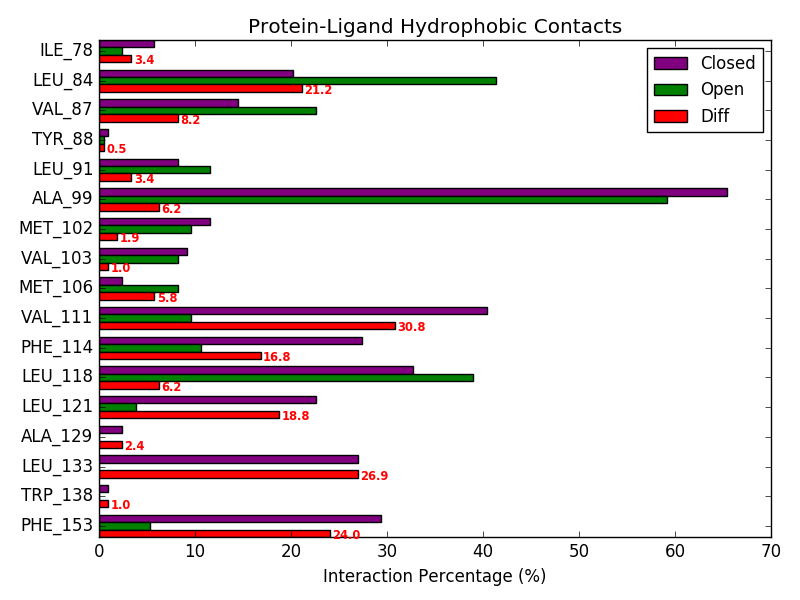
\includegraphics[scale=0.6]{Figures/ContactMap/benzene-hexylbenzene_CM_def.png}}
\end{subfigure}
\centering
\begin{subfigure}{\textwidth}
  \centering
  \frame{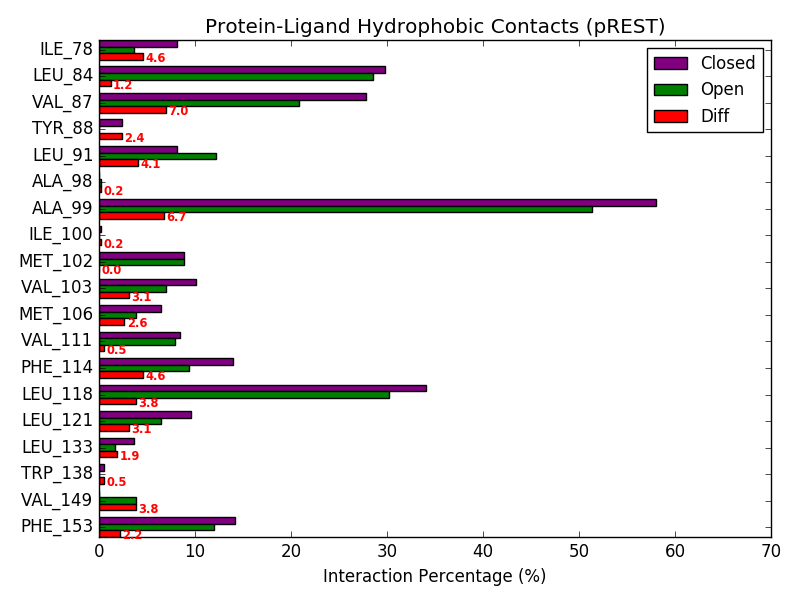
\includegraphics[scale=0.6]{Figures/ContactMap/benzene-hexylbenzene_CM_pREST.png}}
\end{subfigure}
\caption{Bar plot of interaction percentage of protein-ligand hydrophobic contacts over the course of a trajectory. 
From the benzene to hexylbenzene transformation, these plots correspond to the hexylbenzene ($\lambda_{11}$) state from closed (purple) and open (green) simulations using the default versus pREST protocols.
The mean absolute difference (MAD) in interaction percentage is represented in red.
MAD for the default protocol is 10.5\% and 2.8\% for the pREST protocol.
}
\label{fig:contactmap}
\end{figure}

\newpage
\subsection{Tables}

\begin{table}[!htb]
\centering
\caption{Closed-Intermediate Transformations\textsuperscript{\emph{a}}}
\label{tbl:C-I}
\begin{tabular}{|c|c|c|c|c|c|c|}
\hline
\textbf{Ligand 1}   & \textbf{Ligand 2}    & \boldmath$\Delta\Delta G_{C}$ & \boldmath$\sigma_{C}$ & \boldmath$\Delta\Delta G_{O}$ & \boldmath$\sigma_{O}$ & \boldmath$\Delta\Delta G_{\varepsilon}$            \\ \hline
benzene         & butylbenzene   & 0.58    & 0.07  & -0.59  & 0.08  & \cellcolor[HTML]{FFCCC9}1.17 \\ \hline
toluene         & butylbenzene   & -0.28   & 0.06  & -1.27  & 0.09  & \cellcolor[HTML]{9AFF99}0.99 \\ \hline
ethylbenzene    & butylbenzene   & 0.24    & 0.06  & -0.23  & 0.07  & \cellcolor[HTML]{9AFF99}0.47 \\ \hline
propylbenzene & butylbenzene   & 0.99    & 0.06  & 0.63   & 0.04  & \cellcolor[HTML]{9AFF99}0.36 \\ \hline
benzene         & sec-butylbenzene & 2.36    & 0.09  & 2.14   & 0.11  & \cellcolor[HTML]{9AFF99}0.22 \\ \hline
toluene         & sec-butylbenzene & 1.47    & 0.07  & 1.14   & 0.08  & \cellcolor[HTML]{9AFF99}0.33 \\ \hline
ethylbenzene    & sec-butylbenzene & 1.90    & 0.08  & 1.77   & 0.08  & \cellcolor[HTML]{9AFF99}0.13 \\ \hline
propylbenzene & sec-butylbenzene & 2.86    & 0.06  & 2.67   & 0.05  & \cellcolor[HTML]{9AFF99}0.19 \\ \hline
\end{tabular}

\textsuperscript{\emph{a}} Calculated free energies and their uncertainties in `closed-intermediate' alchemical transformations from simulations that were started from the protein closed state(\boldmath$\Delta\Delta G_{C}$) versus the protein open state(\boldmath$\Delta\Delta G_{O}$).
Free energies are in units of kcal/mol. 
The inconsistency(\boldmath$\Delta\Delta G_{\varepsilon}$) is obtained from the difference in the relative free energies between protein closed and open simulations. 
Inconsistency is highlighted red or green if above or below 1 kcal/mol, respectively.
RMSI is 0.6 kcal/mol.
Table is represented in Fig~\ref{fig:C2I_xyplot}.
\end{table}

\begin{table}[!htb]
 \centering
 \caption{Closed-Intermediate Transformations pREST\textsuperscript{\emph{a}}} 
 \label{tbl:C-I_pREST}
 \begin{tabular}{|c|c|c|c|c|c|c|}
 \hline
 \textbf{Ligand 1}       & \textbf{Ligand 2}    & \boldmath$\Delta\Delta G_{C}$ & \boldmath$\sigma_{C}$ & \boldmath$\Delta\Delta G_{O}$ & \boldmath$\sigma_{O}$ & \boldmath$\Delta\Delta G_{\varepsilon}$ \\ \hline
benzene         & butylbenzene   & -0.07   & 0.10     & -0.72     & 0.12     & \cellcolor[HTML]{9AFF99}0.65 \\ \hline
toluene         & butylbenzene   & 0.89    & 0.10     & -0.42     & 0.08     & \cellcolor[HTML]{FFCCC9}1.31 \\ \hline
ethylbenzene    & butylbenzene   & -0.20   & 0.09     & -0.43     & 0.08     & \cellcolor[HTML]{9AFF99}0.23 \\ \hline
propylbenzene & butylbenzene   & 1.02    & 0.06     & 0.49      & 0.06     & \cellcolor[HTML]{9AFF99}0.53 \\ \hline
benzene         & sec-butylbenzene & 0.45    & 0.08     & 1.34      & 0.12     & \cellcolor[HTML]{9AFF99}0.89 \\ \hline
toluene         & sec-butylbenzene & 0.60    & 0.12     & 0.60      & 0.10     & \cellcolor[HTML]{9AFF99}0.00 \\ \hline
ethylbenzene    & sec-butylbenzene & 1.09    & 0.10     & 1.69      & 0.09     & \cellcolor[HTML]{9AFF99}0.60 \\ \hline
propylbenzene & sec-butylbenzene & 1.88    & 0.07     & 3.05      & 0.07     & \cellcolor[HTML]{FFCCC9}1.17 \\ \hline
 \end{tabular}

\textsuperscript{\emph{a}} Calculated free energies and their uncertainties in `closed-intermediate' alchemical transformations from `pREST' simulations that were started from the protein closed state(\boldmath$\Delta\Delta G_{C}$) versus the protein open state(\boldmath$\Delta\Delta G_{O}$).
Free energies were calculated using frames from 0 to 5ns. 
Free energies are in units of kcal/mol.
The inconsistency(\boldmath$\Delta\Delta G_{\varepsilon}$) is obtained from the difference in the relative free energies between protein closed and open simulations. 
Inconsistency is highlighted red or green if above or below 1 kcal/mol, respectively.
RMSI is 0.79 kcal/mol.
Table is represnted in Fig~\ref{fig:C2I_xyplot_pREST}.
 \end{table}

\begin{table}[!htb]
\centering
\caption{Closed-Intermediate Transformations pREST Extended\textsuperscript{\emph{a}},\textsuperscript{\emph{b}}}
\label{tbl:C-I_pRESText}
\begin{tabular}{|c|c|c|c|c|c|c|}
\hline
\textbf{Ligand 1}       & \textbf{Ligand 2}    & \boldmath$\Delta\Delta G_{C}$ & \boldmath$\sigma_{C}$ & \boldmath$\Delta\Delta G_{O}$ & \boldmath$\sigma_{O}$ & \boldmath$\Delta\Delta G_{\varepsilon}$ \\ \hline
benzene          & butylbenzene   & -1.14\textsuperscript{\emph{b}}    & 0.09  & -0.72   & 0.12  & \cellcolor[HTML]{9AFF99}0.42 \\ \hline
toluene          & butylbenzene   & -0.62\textsuperscript{\emph{b}}    & 0.09  & -0.96\textsuperscript{\emph{a}}  & 0.09  & \cellcolor[HTML]{9AFF99}0.34 \\ \hline
ethylbenzene     & butylbenzene   & -0.20     & 0.09  & -0.43   & 0.08  & \cellcolor[HTML]{9AFF99}0.23 \\ \hline
propylbenzene  & butylbenzene   & 0.51\textsuperscript{\emph{b}}     & 0.06  & 0.49    & 0.06  & \cellcolor[HTML]{9AFF99}0.02 \\ \hline
benzene          & sec-butylbenzene & 0.45      & 0.08  & 1.34    & 0.12  & \cellcolor[HTML]{9AFF99}0.89 \\ \hline
toluene          & sec-butylbenzene & 0.60      & 0.12  & 0.60    & 0.10  & \cellcolor[HTML]{9AFF99}0.00 \\ \hline
ethylbenzene     & sec-butylbenzene & 1.09      & 0.10  & 1.69    & 0.09  & \cellcolor[HTML]{9AFF99}0.60 \\ \hline
propylbenzene  & sec-butylbenzene & 1.88      & 0.07  & 1.84\textsuperscript{\emph{b}}   & 0.06  & \cellcolor[HTML]{9AFF99}0.04 \\ \hline
\end{tabular}
 
\textsuperscript{\emph{a}} Calculated free energies and their uncertainties in `closed-intermediate' alchemical transformations from `pREST' simulations that were started from the protein closed state(\boldmath$\Delta\Delta G_{C}$) versus the protein open state(\boldmath$\Delta\Delta G_{O}$).
Free energies were calculated using frames from 15 to 25ns. 
Free energies are in units of kcal/mol.
The inconsistency(\boldmath$\Delta\Delta G_{\varepsilon}$) is obtained from the difference in the relative free energies between protein closed and open simulations. 
Inconsistency is highlighted red or green if above or below 1 kcal/mol, respectively.
RMSI is 0.43 kcal/mol.
Table is represnted in Fig~\ref{fig:C2I_xyplot_pREST}.

\textsuperscript{\emph{b}} Only these alchemical transformations were extended up to 25ns of simulation time in order to lower the inconsistency and error with experiment.
\end{table}

\begin{table}[!htb]
\centering
\caption{Closed-Open Transformations\textsuperscript{\emph{a}}}
\label{tbl:C-O}
\begin{tabular}{|c|c|c|c|c|c|c|}
\hline
\textbf{Ligand 1}       & \textbf{Ligand 2}    & \boldmath$\Delta\Delta G_{C}$ & \boldmath$\sigma_{C}$ & \boldmath$\Delta\Delta G_{O}$ & \boldmath$\sigma_{O}$ & \boldmath$\Delta\Delta G_{\varepsilon}$ \\ \hline
benzene         & pentylbenzene & 2.36       & 0.12  & -1.33  & 0.10  & \cellcolor[HTML]{FFCCC9}3.69 \\ \hline
toluene         & pentylbenzene & 1.77       & 0.09  & 0.34   & 0.10  & \cellcolor[HTML]{FFCCC9}1.43 \\ \hline
ethylbenzene    & pentylbenzene & 2.45       & 0.08  & 0.46   & 0.09  & \cellcolor[HTML]{FFCCC9}1.99 \\ \hline
propylbenzene & pentylbenzene & 3.46       & 0.08  & -0.22  & 0.07  & \cellcolor[HTML]{FFCCC9}3.68 \\ \hline
benzene         & hexylbenzene  & 4.13       & 0.16  & -0.61  & 0.15  & \cellcolor[HTML]{FFCCC9}4.74 \\ \hline
toluene         & hexylbenzene  & 2.90       & 0.13  & -1.63  & 0.08  & \cellcolor[HTML]{FFCCC9}4.53 \\ \hline
ethylbenzene    & hexylbenzene  & 3.63       & 0.11  & -0.76  & 0.09  & \cellcolor[HTML]{FFCCC9}4.39 \\ \hline
propylbenzene & hexylbenzene  & 5.85       & 0.10  & 0.13   & 0.06  & \cellcolor[HTML]{FFCCC9}5.72 \\ \hline
\end{tabular}

\textsuperscript{\emph{a}} Calculated free energies and their uncertainties in `closed-open' alchemical transformations from simulations that were started from the protein closed state(\boldmath$\Delta\Delta G_{C}$) versus the protein open state(\boldmath$\Delta\Delta G_{O}$).
Free energies were calculated using frames from 0 to 5ns.  
Free energies are in units of kcal/mol. 
The inconsistency(\boldmath$\Delta\Delta G_{\varepsilon}$) is obtained from the difference in the relative free energies between protein closed and open simulations. 
Inconsistency is highlighted red or green if above or below 1 kcal/mol, respectively.
RMSI is 4.0 kcal/mol.
Table is represented in Fig~\ref{fig:C2O_xyplot}.
\end{table}

\begin{table}[!htb]
\centering
\caption{Closed-Open Transformations pREST\textsuperscript{\emph{a}}}
\label{tbl:C-O_pREST}
\begin{tabular}{|c|c|c|c|c|c|c|}
\hline
\textbf{Ligand 1}       & \textbf{Ligand 2}    & \boldmath$\Delta\Delta G_{C}$ & \boldmath$\sigma_{C}$ & \boldmath$\Delta\Delta G_{O}$ & \boldmath$\sigma_{O}$ & \boldmath$\Delta\Delta G_{\varepsilon}$\\ \hline
benzene         & pentylbenzene & 1.49       & 0.13     & 0.07   & 0.10     & \cellcolor[HTML]{FFCCC9}1.42 \\ \hline
toluene         & pentylbenzene & 1.41       & 0.12     & 0.79   & 0.13     & \cellcolor[HTML]{9AFF99}0.62 \\ \hline
ethylbenzene    & pentylbenzene & 2.90       & 0.10     & 1.23   & 0.09     & \cellcolor[HTML]{FFCCC9}1.67 \\ \hline
propylbenzene & pentylbenzene & 4.25       & 0.09     & 1.01   & 0.07     & \cellcolor[HTML]{FFCCC9}3.24 \\ \hline
benzene         & hexylbenzene  & 2.75       & 0.14     & 1.25   & 0.11     & \cellcolor[HTML]{FFCCC9}1.50 \\ \hline
toluene         & hexylbenzene  & 3.22       & 0.11     & -1.15  & 0.11     & \cellcolor[HTML]{FFCCC9}4.37 \\ \hline
ethylbenzene    & hexylbenzene  & 3.34       & 0.12     & -0.22  & 0.11     & \cellcolor[HTML]{FFCCC9}3.56 \\ \hline
propylbenzene & hexylbenzene  & 4.93       & 0.12     & 1.21   & 0.11     & \cellcolor[HTML]{FFCCC9}3.72 \\ \hline
\end{tabular}

\textsuperscript{\emph{a}} Calculated free energies and their uncertainties in `closed-open' alchemical transformations from `pREST' simulations that were started from the protein closed state(\boldmath$\Delta\Delta G_{C}$) versus the protein open state(\boldmath$\Delta\Delta G_{O}$).
Free energies are in units of kcal/mol. 
The inconsistency(\boldmath$\Delta\Delta G_{\varepsilon}$) is obtained from the difference in the relative free energies between protein closed and open simulations. 
The inconsistency is highlighted red or green if above or below 1 kcal/mol, respectively.
RMSI is 2.82 kcal/mol. 
\end{table}

\begin{table}[!htb]
\centering
\caption{Closed-Open Transformations pREST Extended\textsuperscript{\emph{a}}}
\label{tbl:C-O_pREST-40-55ns}
\begin{tabular}{|c|c|c|c|c|c|c|}
\hline
\textbf{Ligand 1}       & \textbf{Ligand 2}    & \boldmath$\Delta\Delta G_{C}$ & \boldmath$\sigma_{C}$ & \boldmath$\Delta\Delta G_{O}$ & \boldmath$\sigma_{O}$ & \boldmath$\Delta\Delta G_{\varepsilon}$ \\ \hline
benzene         & pentylbenzene & 1.37       & 0.08     & 1.41    & 0.08      & \cellcolor[HTML]{9AFF99}0.04 \\ \hline
toluene         & pentylbenzene & 1.08       & 0.08     & 0.81    & 0.07      & \cellcolor[HTML]{9AFF99}0.27 \\ \hline
ethylbenzene    & pentylbenzene & 1.71       & 0.08     & 1.50    & 0.07      & \cellcolor[HTML]{9AFF99}0.21 \\ \hline
propylbenzene & pentylbenzene & 3.20       & 0.06     & 2.34    & 0.05      & \cellcolor[HTML]{9AFF99}0.86 \\ \hline
benzene         & hexylbenzene  & 2.15       & 0.09     & 1.14    & 0.08      & \cellcolor[HTML]{FFCCC9}1.01 \\ \hline
toluene         & hexylbenzene  & 0.32       & 0.10     & 1.10    & 0.07      & \cellcolor[HTML]{9AFF99}0.78 \\ \hline
ethylbenzene    & hexylbenzene  & 1.96       & 0.08     & 2.17    & 0.07      & \cellcolor[HTML]{9AFF99}0.21 \\ \hline
propylbenzene & hexylbenzene  & 3.38       & 0.07     & 3.12    & 0.06      & \cellcolor[HTML]{9AFF99}0.26 \\ \hline
\end{tabular}

\textsuperscript{\emph{a}} Calculated free energies and their uncertainties in `closed-open' alchemical transformations from extended `pREST' simulations that were started from the protein closed state(\boldmath$\Delta\Delta G_{C}$) versus the protein open state(\boldmath$\Delta\Delta G_{O}$). 
Free energies are in units of kcal/mol.
Free energies were calculated using frames from 40 to 55ns. 
The inconsistency(\boldmath$\Delta\Delta G_{\varepsilon}$) is obtained from the difference in the relative free energies between protein closed and open simulations. 
Inconsistency is highlighted red or green if above or below 1 kcal/mol, respectively.
RMSI is 0.57 kcal/mol.
Table is represented in Fig~\ref{fig:C2O_xyplot_pREST}.
\end{table}

\begin{table}[!htb]
\centering
\caption{Experimental Ligand Transformations\textsuperscript{\emph{a}}}
\label{tbl:exp_set}
\begin{tabular}{|c|c|c|c|c|c|c|c|}
\hline
\textbf{Ligand 1} & \textbf{Ligand 2}  & \boldmath$\Delta G_{exp}$  & \boldmath$\sigma_{exp}$ & \boldmath$\Delta\Delta G_{C}$ & \boldmath$\sigma_{C}$ & \boldmath$\Delta\Delta G_{O}$ & \boldmath$\sigma_{O}$ \\ \hline
benzene         & toluene         & -0.33        & 0.16            & 0.71       & 0.04          & 0.59       & 0.05          \\ \hline
benzene         & ethylbenzene    & -0.19        & 0.17            & 0.15       & 0.05          & -0.09      & 0.06          \\ \hline
benzene         & propylbenzene & -1.36        & 0.16            & -0.82      & 0.06          & -0.69      & 0.08          \\ \hline
benzene         & butylbenzene  & -1.51        & 0.16            & 0.58       & 0.07          & -0.59      & 0.08          \\ \hline
toluene         & ethylbenzene    & -0.24        & 0.08            & -0.59      & 0.04          & -0.40      & 0.05          \\ \hline
toluene         & propylbenzene & -1.03        & 0.04            & -2.21      & 0.05          & -0.89      & 0.05          \\ \hline
toluene         & butylbenzene  & -1.18        & 0.04            & -0.28      & 0.06          & -1.27       & 0.09         \\ \hline
ethylbenzene    & propylbenzene & -0.79        & 0.07            & -0.86      & 0.05          & -0.80       & 0.03         \\ \hline
ethylbenzene    & butylbenzene  & -0.94        & 0.07            & 0.24       & 0.06          & -0.23      & 0.07          \\ \hline
propylbenzene & butylbenzene  & -0.15        & 0.03            & 0.99       & 0.06          & 0.63       & 0.04          \\ \hline
\end{tabular}

\textsuperscript{\emph{a}} Experimental and calculated free energies with their uncertainties in alchemical transformations involving ligands with available experimental affinities.
Calculated free energies are from simulations that were started from the protein closed state(\boldmath$\Delta\Delta G_{C}$) versus the protein open state(\boldmath$\Delta\Delta G_{O}$). 
Free energies are in units of kcal/mol.
Here, we compare \boldmath$\Delta\Delta G_{C}$ and \boldmath$\Delta\Delta G_{O}$ against \boldmath$\Delta G_{exp}$ to compute the error with experiment.
RMSE is 1.0 kcal/mol and 0.58 kcal/mol for closed and open simulations, respectively.
RMSI is 0.68 kcal/mol.
Table is represented in Fig~\ref{fig:exp_xyplot}.
\end{table}

\begin{table}[!htb]
\centering
\caption{Experimental Ligand Transformations pREST\textsuperscript{\emph{a}}}
\label{tbl:exp_pREST_set}
\begin{tabular}{|c|c|c|c|c|c|c|c|}
\hline
\textbf{Ligand 1} & \textbf{Ligand 2} & \boldmath$\Delta G_{exp}$  & \boldmath$\sigma_{exp}$ & \boldmath$\Delta\Delta G_{C}$ & \boldmath$\sigma_{C}$ & \boldmath$\Delta\Delta G_{O}$ & \boldmath$\sigma_{O}$ \\ \hline
benzene         & toluene         & -0.33 & 0.16  & 0.10  & 0.08  & 0.31  & 0.06          \\ \hline
benzene         & ethylbenzene    &-0.19  & 0.17  & -0.20 & 0.08  & -0.62 & 0.08          \\ \hline
benzene         & propylbenzene & -1.36 & 0.16  & -1.57 & 0.09  & -1.26 & 0.09         \\ \hline
benzene         & butylbenzene  & -1.51 & 0.16  & -1.14 & 0.11  & -0.72 & 0.12         \\ \hline
toluene         & ethylbenzene    & -0.24 & 0.08  & -0.84 & 0.07  & -0.83 & 0.07          \\ \hline
toluene         & propylbenzene & -1.03 & 0.04  & -1.91 & 0.09  & -1.44 & 0.08          \\ \hline
toluene         & butylbenzene  & -1.18 & 0.04  & -0.62 & 0.09  & -0.96 & 0.09          \\ \hline
ethylbenzene    & propylbenzene & -0.79 & 0.07  & -1.08 & 0.07  & -0.80 & 0.06         \\ \hline
ethylbenzene    & butylbenzene  & -0.94 & 0.07  & -0.20 & 0.09  & -0.43 & 0.08         \\ \hline
propylbenzene & butylbenzene  & -0.15 & 0.03  & 0.51  & 0.06  & 0.49  & 0.06       \\ \hline
\end{tabular}

\textsuperscript{\emph{a}} Experimental and calculated free energies with their uncertainties in alchemical transformations involving ligands with available experimental affinities.
Calculated free energies are from `pREST' simulations that were started from the protein closed state(\boldmath$\Delta\Delta G_{C}$) versus the protein open state(\boldmath$\Delta\Delta G_{O}$). 
Free energies are in units of kcal/mol.
Here, we compare \boldmath$\Delta\Delta G_{C}$ and \boldmath$\Delta\Delta G_{O}$ against \boldmath$\Delta G_{exp}$ to compute the error with experiment.
RMSE is 0.54 kcal/mol and 0.50 kcal/mol for closed and open simulations, respectively.
RMSI is 0.31 kcal/mol.
Table is represented in Fig~\ref{fig:exp_xyplot_pREST}.
\end{table}

\clearpage
\subsection*{Data Sets and Analysis Tool Download}
All related data sets and analysis tools are available online and described below.
The files can be downloaded at http://n2t.net/ark:/b7280/d1js3b (doi:10.7280/D1JS3B). 
\begin{description}
\item [Prepared protein-ligand crystal structures:]\texttt{xtal\_prepped.tar.gz}\\
Contains the reference protein-ligand crystal structures that have been aligned and prepared through the `Protein Preparation Wizard' tool as \texttt{.mae} files.
\item [RMSD analysis:]\texttt{scripts.tar.gz}\\
Contains the scripts \texttt{RMSD-analysis.tcl} and \texttt{plot-RMSD.py} used for RMSD analysis. A \texttt{README.txt} file has been provided which details how to generate the RMSD/time and Colormap plots found in the paper. 
\item [FEP data:]\texttt{C-I\_default.tar.gz}, \texttt{C-I\_pPREST.tar.gz}, \texttt{C-O\_default.tar.gz}, \\ \texttt{C-O\_pREST.tar.gz}, \texttt{EXP\_default.tar.gz,} and \texttt{EXP\_pREST.tar.gz}\\
Contains archived data from the FEP calculations for each alchemical transformation set, where within each archived set are directories for individual FEP calculations. These contain input \texttt{.mae} files containing the protein/ligand structures, the simulation configuration \texttt{.msj} files, energy files, and a \texttt{README.txt} that summarizes information about each FEP calculation. Complete trajectories are included.
\end{description}


\chapter{Computational studies of Diphtheria Toxin T Domain: role of acidic residue E362 in membrane-protein insertion and pore formation.} \label{DTT}
\small{Authors: Nathan M. Lim, J. Alfredo Freites, Linh P. Nguyen, Douglas J. Tobias, David L. Mobley}\\
\emph{Excerpt from: `Refining Protein Penetration into the Lipid Bilayer Using Fluorescence Quenching and Molecular Dynamics Simulations: The Case of Diphtheria Toxin Translocation Domain' \cite{Kyrychenko2018}}\\
\emph{J. Mem. Bio., 2018, 251 (9), pp 379--391 \\
\doi{doi:10.1007/s00232-018-0030-2}\\Publication Date (Web): March 17, 2018}


\begin{figure}[H]
\centering
\frame{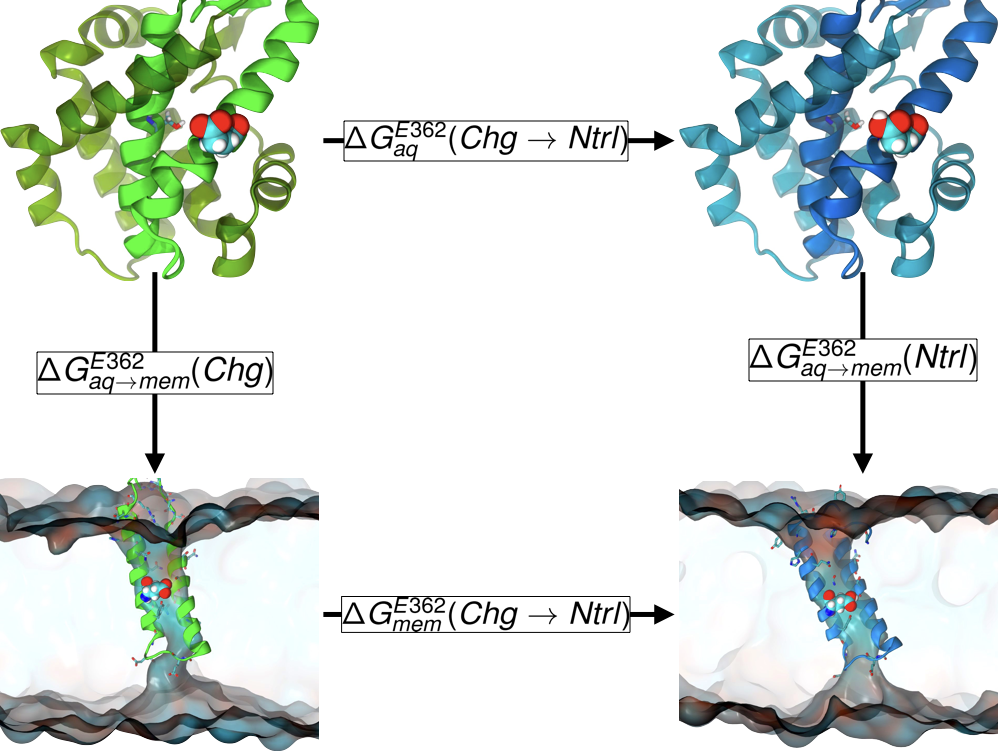
\includegraphics[width=\linewidth,]{Figures/DTT/thermo_cycle.png}}
\caption[Thermodynamic cycle for membrane-protein insertion]{Thermodynamic cycle for calculating membrane-protein insertion free energies of DTT for neutralized E362 relative to charged E362. The vertical legs relate to the membrane insertion free energies of DTT which is obtained from the equivalent horizontal legs calculated from the alchemical free energy calculations. Residue E362 is represented with van der Waals spheres in each image. For figures of the protein, the TH8-TH9 helices are shaded differently from the rest of the protein and S336 is displayed to illustrate its position on the TH8 helix relative to E362.}
\label{fig:dtt_thermo_cycle}
\end{figure}


\section{Introduction}
Recent experimental studies on the Diphtheria Toxin T domain (DTT) characterized the importance in protonation of acidic residue E362 in the membrane insertion process \cite{ghatak2015role}.
Through mutagenesis studies of E362Q--whereby the charge is effectively removed--it was demonstrated that this residue plays a key role in the insertion of the TH8-TH9 helices.
In order to quantitatively understand the role of the charged residue E362 and the energetics in the insertion mechanism of DTT, we compute the membrane-protein insertion free energy.
In this study, we utilize an all-atom (explicit solvent \& membrane) molecular dynamics (MD) simulation with the alchemical free-energy perturbation (FEP) approach.
Here, we compute the change in free energies between the charged and neutral states of E362 from simulations carried out in solution and membrane environments.
Our free energy predictions indicate high favorability (approximately -6$\frac{kcal}{mol}$) for neutral E362 in the membrane-protein insertion pathway--which seems consistent with experimental mutagenesis results \cite{ghatak2015role}.
Additional profiling of the pore formed by DTT indicates neutralized E362 induces larger perturbations to the membrane, providing further evidence E362 plays a key role during insertion.

\section{Methods}
\subsection{Molecular Dynamics simulation \& Free energy calculation protocols}
The initial protein configurations were based on the crystal structure of wild-type diphtheria toxin (PDB ID 1f0l). 
The protein in the solution simulation system consisted of the full T domain (residues 202–378), and in the membrane system, of the TH8–TH9 hairpin (residues 319–380). 
TH8 is a hydrophobic helix while TH9 exhibits a significant hydro- phobic moment. 
In the crystal structure TH8 appears fully protected by the rest of the T domain, therefore, in order to produce an initial protein configuration with favorable interactions with the membrane environment, we rotated TH9 180° about its principal axis so as to orient the polar face towards TH8 and away from the lipid bilayer hydrocarbon core.
Titratable side chains were modeled consistent with neutral pH in the solution system, and with acidic pH in the membrane system. 
Specifically, in the solution system, all histidine residues were neutralized and acidic residues were ionized. 
In the membrane system, all histidine residues were charged and, except for E362, all acidic residues were neutralized. 
The solution simulation system was generated using VMD \cite{humphrey1996vmd}. 
The final solution system consisted of one T domain, 2768 waters and, 10 counterions for a total of 11,032 atoms. 
The membrane system was set up by inserting the TH8–TH9 hairpin in a 1:1 POPC–POPG bilayer in excess water using the CHARMM–GUI membrane builder \cite{jo2009charmm} and VMD. 
The final mem- brane system consisted of one TH8–TH9 hairpin, 250 lipids, 11,724 waters, and 122 counterions for a total of 68,872 atoms. 
Equilibration simulations were carried out at con- stant pressure (1 atm) and temperature (300 K) for approximately 40 and 113 ns for the aqueous and membrane systems, respectively.

The simulations were run with the NAMD (v2.11) software package \cite{phillips2005scalable} under three-dimensional periodic boundary conditions (PBC). 
The protein was modeled using the CHARMM22 force field \cite{mackerell1998all}
The CHARMM36 force field was used for lipids \cite{klauda2010update} and the TIP3P \cite{jorgensen1983comparison} model was used for water. 
A reversible multiple-time- step algorithm \cite{grubmuller1991generalized} was used to integrate the equations of motion with a time step of 4 fs for the long- range electrostatic forces, and 2 fs for the short-range non- bonded forces and the bonded forces. 
The smooth particle mesh Ewald method \cite{essmann1995smooth} was used to calculate electrostatic interactions. 
The short-range interactions were cutoff at 12 Å using a force-based switching scheme.
All bond lengths involving hydrogen atoms were held fixed using the SHAKE \cite{ryckaert1977numerical} and SETTLE \cite{miyamoto1992settle} algorithms. 
A Langevin dynamics scheme was used for thermostating. Nosé–Hoover–Langevin pistons were used for pressure contro (\cite{feller1995constant};\cite{martyna1994constant}).

Alchemical free energy calculations were divided into 40 equally spaced windows with production simulations running for 5 ns per stage, giving a total of 200 ns for each system.
Each production run was preceded by an equilibration protocol consisting of 10,000 steps of conjugate-gradient energy minimization and a 1 ns MD run. 
Free energies were calculated using Bennett Acceptance Ratio \cite{bennett1976efficient} as implemented by the PyMBAR program \cite{shirts2008statistically, chodera2007use}.
Corrections to the final free energies were performed using a scheme based on a continuum-electrostatics analysis, which corrects for spuri- ous interactions encountered when simulations are carried out with periodic boundary conditions \cite{rocklin2013calculating}.

Trajectory analyses were performed using VMD and MDtraj \cite{mcgibbon2015mdtraj}.
Molecular graphics were generated using VMD \cite{humphrey1996vmd}.
Analysis of the pore resulting from the TH8–TH9 hairpin insertion in the membrane was done using dxTuber (v0.28) \cite{raunest2011dxtuber}.
OpenDX density maps were generated using the VolMap(v1.1) plugin in VMD with the following settings: resolution: 1.0 Å atom size: 1.0 × radius, weights: mass
Density maps were combined over the final 64 ns from the membrane MD simulations.
For analysis with dxTuber, we used a combination of two settings: (1) time-averaged for both the protein and solvent and (2) minimum protein density and time-averaged solvent density. Trajectory frames were aligned by the hairpin backbone using the starting frame as reference and then wrapped about the hairpin’s center of mass using MDtraj \cite{mcgibbon2015mdtraj}.

\section{Results \& Discussion}

\begin{table}[H]
\centering
\caption[Initial and corrected free energies]{Initial and corrected\cite{rocklin2013calculating} free energies obtained from alchemical free energy calculations which transformed E362 from charged to neutral in both the aqueous and membrane environments. The membrane-protein insertion free energies are obtained from the difference in free energies between the two environments.}
\label{tbl:dtt_ddG}
\begin{tabular}{|c|c|c|}
\hline
& \boldmath$\Delta G\frac{kcal}{mol}$   & \boldmath$\Delta G\frac{kcal}{mol}$ Corrected     \\ \hline
$\Delta G_{mem}^{E362}(Chg\rightarrow Ntrl)$ & 84.4 & 93.3 (+/- 0.3) \\ \hline
$\Delta G_{aq}^{E362}(Chg\rightarrow Ntrl)$  & 86.0 & 99.5 (+/- 0.2) \\ \hline
$\Delta\Delta G_{aq\rightarrow mem}^{E362}(Ntrl)$ & -1.6 & -6.2 (+/- 0.4) \\ \hline
\end{tabular}
\end{table}

\subsection{Free Energies indicate high favorability for neutralized E362.}
In our free energy calculations, we alchemically transform the glutamic acid residue at position 362 from its charged to neutral state by effectively creating or annihilating a proton on the terminal oxygen atom, denoted as OE2 from the CHARMM 22 topology.
Our initial state is with the charged residue in the aqueous solution and our end state is that of the neutral residue within the membrane environment. 
To determine the T-domain insertion free energies, we apply the thermodynamic cycle illustrated in Figure \ref{fig:dtt_thermo_cycle} and obtain equation \ref{eqn:dtt_eqn1}.
Here, we define our four terms: $\Delta G_{aq}^{E362}(Chg\rightarrow Ntrl)$ represents the change in free energy of altering the charged residue E362 to neutral in the aqueous environment while $\Delta G_{mem}^{E362}(Chg\rightarrow Ntrl)$ represents the same charge change but in the membrane environment.
The membrane-protein insertion free energy is represented by the terms $\Delta G_{aq\rightarrow mem}^{E362}(Ntrl)$ and $\Delta G_{aq\rightarrow mem}^{E362}(Chg)$, whereby residue E362 is either in the neutral (Ntrl) state or the charged (Chg) state.
\begin{equation}
  0  = \Delta G_{aq}^{E362}(Chg\rightarrow Ntrl) + \Delta G_{aq\rightarrow mem}^{E362}(Ntrl) - \Delta G_{mem}^{E362}(Chg\rightarrow Ntrl) - \Delta G_{aq\rightarrow mem}^{E362}(Chg)
  \label{eqn:dtt_eqn1}
\end{equation}
From rearranging, we show that the free energy difference from insertion of the neu- tral versus charged system is equivalent to the free energy change resulting from the perturbation of the residue in the aqueous versus membrane environment (Eq. 3).  (eqn.~\ref{eqn:dtt_eqn2}).
\begin{equation}
  \Delta G_{aq\rightarrow mem}^{E362}(Ntrl) - \Delta G_{aq\rightarrow mem}^{E362}(Chg)  =  \Delta G_{mem}^{E362}(Chg\rightarrow Ntrl) - \Delta G_{aq}^{E362}(Chg\rightarrow Ntrl)
  \label{eqn:dtt_eqn2}
\end{equation}
Thus, the total membrane-protein insertion free energy can be obtained from either pair of terms.
Since we cannot conduct MD simulations corresponding to the vertical legs from Figure \ref{fig:dtt_thermo_cycle} to obtain the free energies denoted in equation \ref{eqn:dtt_eqn3}, we instead obtain the insertion free energy from the equivalent terms in the cycle.
Thus, from equation \ref{eqn:dtt_eqn4}, the total insertion free energy can obtained from the MD free energy simulations where we perturb the residue in both the aqueous and membrane environments.
\begin{equation}
  \Delta\Delta G_{aq\rightarrow mem}^{E362}(Ntrl)  =  \Delta G_{aq\rightarrow mem}^{E362}(Ntrl) - \Delta G_{aq\rightarrow mem}^{E362}(Chg)
  \label{eqn:dtt_eqn3}
\end{equation}
\begin{equation}
  \Delta\Delta G_{aq\rightarrow mem}^{E362}(Ntrl)  =  \Delta G_{mem}^{E362}(Chg\rightarrow Ntrl) - \Delta G_{aq}^{E362}(Chg\rightarrow Ntrl)
  \label{eqn:dtt_eqn4}
\end{equation}

From our calculations (Table \ref{tbl:dtt_ddG}),the free energy change obtained from alchemically creating a proton to neutralize the charged glutamic residue was $+84.4\frac{kcal}{mol}$ in the membrane and $+86.0\frac{kcal}{mol}$ in the aqueous environment, yielding a final insertion free energy of $-1.6\frac{kcal}{mol}$.
As our simulated system was neutralized with counterions when E362 was charged, the alchemical modification being made here results in the overall system becoming non-neutral.
This gives rise to significant artifacts arising from self-interactions through neighboring periodic copies, which can dramatically impact our free energy differences\cite{rocklin2013calculating}.
A correction scheme for the self-interactions has been previously described in a similar membrane-insertion free energy study, conducted on outer membrane phospholipase A (OmpLA) \cite{gumbart2012determination}.
In this scheme described by Gumbart and Roux, they intentionally neglect the self-interaction from the charged residue and its periodic replicas--on account of the term being negligible due to the pore waters shielding the charge.
As our simulations of T-domain involve a much narrower pore and thus were uncertain if water would effectively shield the charge, we employed a more thorough correction scheme based off a continuum-electrostatics analysis\cite{rocklin2013calculating}.
After applying the analytical continuum-electrostatics scheme described by Rocklin et. al, our corrected insertion free energy was $-6.2 (+/-0.4)\frac{kcal}{mol}$, which suggests high favorability for the neutralized residue in the membrane insertion pathway.

\subsection{Neutralized E362 produces a larger membrane pore.}
We have examined the effect of protonation state of E362 on the local perturbation of the bilayer. 
Through time-averaged density maps of the protein and solvent over the course of the MD simulations, we show that the pore created by T-domain TH8–9 hairpin and the inner tunnel-like cavity are larger when residue E362 is neutralized. 
Thus, we provide supporting evidence on the importance of residue E362 and its pH-dependent conformational switching for perturbing the membrane to allow for insertion.

\begin{figure}[H]
\centering
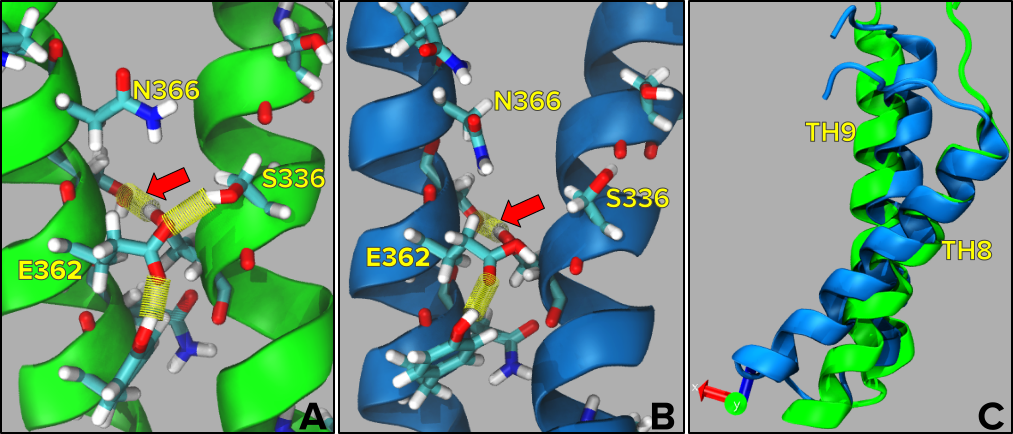
\includegraphics[width=\linewidth,]{Figures/DTT/hbonds_compare.png}
\caption[H-Bonds in DTT TH8-TH9 helices]{Hydrogen bond network between the TH8-TH9 helices involving residues S336, S337, E362, S363, and N366. The red arrow points to the H-bond formed between residues S337/S363 which are the two closest points of contacts between the helices. When E362 is charged (Fig.\ref{fig:dtt_hbonds}A; green), residues N366/S336 are oriented inward but are flipped away when E362 is neutral (Fig.\ref{fig:dtt_hbonds}B; blue). Fig. \ref{fig:dtt_hbonds}C shows the shift of the TH8 helix when E362 is charged by overlaying the protein structure from neutralized E362.}
\label{fig:dtt_hbonds}
\end{figure}

From our MD simulations, we found that the exposure of the charge on residue E362 within the membrane environment results in the two helices moving closer together to effectively shield the unfavorable charge in the center of the surrounding non-polar membrane environment. 
When residue E362 is charged, the two helices are pulled together by formation of a hydrogen bond network primarily involving residues surrounding E362.
From Figure \ref{fig:dtt_hbonds}, we show that resi- dues S336 and S337 on the TH8 helix are oriented inward in order to more closely interact with residues N366, S363, and charged E362 on the opposing TH9 helix.
From calculating the percent occupancy of hydrogen bond contacts between S336 and S363—the two closest residues on opposing helices-—we find that when residue E362 is neutral, hydrogen bonding occurs in roughly 57\% of trajectory frames, but when E362 is charged the hydrogen bonding occurs in approximately 88\% of the trajectory frames.
Our analysis of the MD trajectories indicates that when E362 is charged, the two helices are drawn closer together, thereby decreasing the overall perturbation to the membrane.
This finding suggests favorability for neutralized over charged E362 during the membrane insertion mechanism as formation of a larger pore could better facilitate delivery of the catalytic domain across the membrane.

\begin{table}[H]
\centering
\caption[Cross-sectional area of DTT pore]{Mean cross-sectional area along the Z-axis of the pore formed by DTT when E362 is charged versus neutral. Calculated from dxTuber\cite{raunest2011dxtuber}, using average solvent densities with average versus minimum protein densities.}
\label{tbl:dtt_pore}
\begin{tabular}{|c|c|c|}
\hline
\textbf{E362 State}  & \boldmath$Avg(\AA^{2})$ & \boldmath$Min(\AA^{2})$ \\ \hline
Neutral & 740 & 318 \\ \hline
Charged & 750 & 217 \\ \hline
\end{tabular}
\end{table}

\begin{figure}[H]
\centering
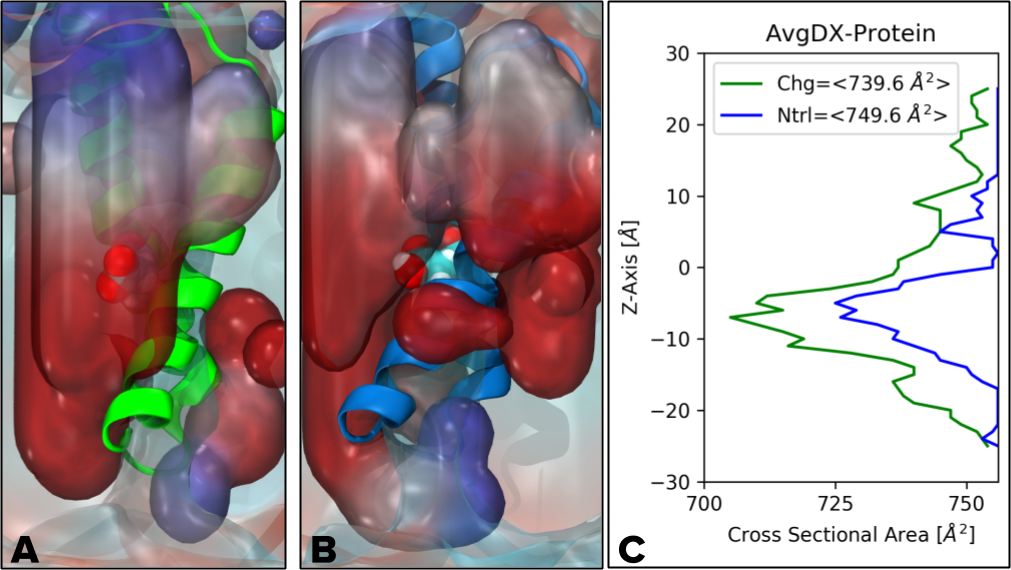
\includegraphics[width=\linewidth,]{Figures/DTT/avgdx.png}
\caption[Solvent accessibility of DTT pore]{Solvent accessibility map using average protein and average solvent densities over the 64ns MD simulation. The time-averaged solvent densities are shown for when E362 is charged (Fig.\ref{fig:dtt_avgdx}A; green) and when E362 is neutral (Fig.\ref{fig:dtt_avgdx}B; blue). Solvent densities are colored red for high density and blue for low density. Fig.\ref{fig:dtt_avgdx}C plots the cross-sectional area along the Z-axis with the mean cross-sectional areas being 750\AA$^2$ for neutral E362 and 740\AA$^2$ for charged E362 (Table \ref{tbl:dtt_pore}).}
\label{fig:dtt_avgdx}
\end{figure}

In order to approximate the pore size from T-domain insertion, we use dxTuber to calculate the cross-sectional area along the membrane normal over the course of the MD trajectories. 
By using the average protein and average solvent densities, we generate a time-averaged map of solvent accessibility around the protein (Fig.\ref{fig:dtt_avgdx}).
Solvent accessibility is colored by according to the averaged density (red=high density; blue=low).
From our analysis (Table \ref{tbl:dtt_pore}), we find that the average cross-sectional area when residue E362 is neutral is 750\AA$^2$ and when charged is 740\AA$^2$.
Next, by using the minimum protein densities with averaged solvent densities, we filter out regions of high protein flexibility.
This yields a map of the areas with maximum solvent accessibility, which appears to map the solvent accessibility of pore interior (Fig.\ref{fig:dtt_mindx}).
The average cross-sectional area through the inner cavity when residue E362 is neutral is 318\AA$^2$ and when charged is 217\AA$^2$.
Both the average and minimum protein profiles indicate the overall pore formed in the membrane by T-domain insertion is greater in size when residue E362 is neutralized.
This analysis provides further evidence that membrane perturba- tion starts with the initial insertion of TH8–9 domain and that E362 may play multiple roles in modulating the inser- tion mechanism of the T-domain.

\begin{figure}[H]
\centering
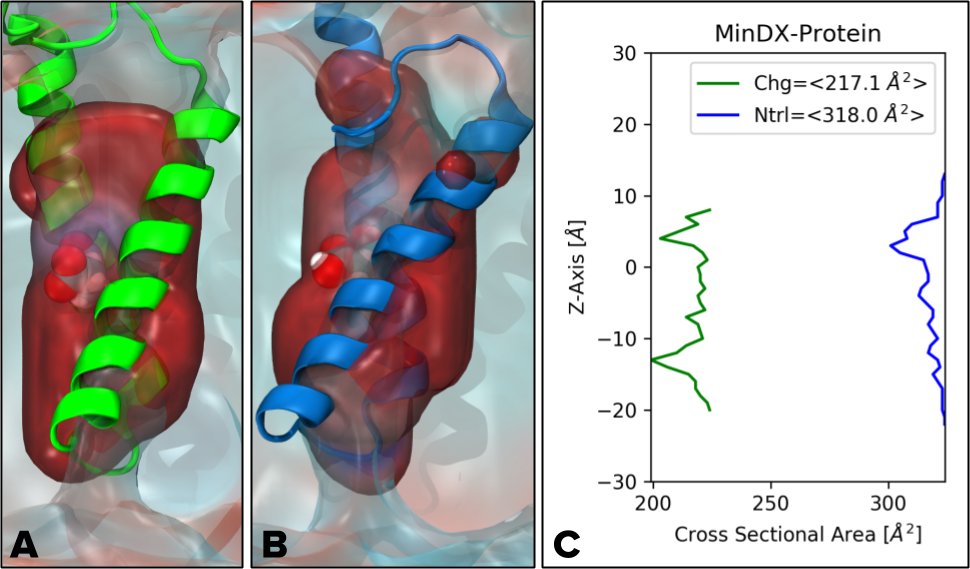
\includegraphics[width=\linewidth,]{Figures/DTT/mindx.png}
\caption[Solvent accesibility map for Charged E362 DTT Pore]{Maximum solvent accessibility map for when E362 is charged (Fig.\ref{fig:dtt_mindx}A; green) and neutral (Fig.\ref{fig:dtt_mindx}B; blue), using minimum protein and average solvent densities over the 64ns MD simulation. Fig.\ref{fig:dtt_mindx}C plots the cross-sectional area along the Z-axis with the mean cross-sectional areas being 318\AA$^2$ for neutral E362 and 217\AA$^2$ for charged E362 (Table \ref{tbl:dtt_pore}).}
\label{fig:dtt_mindx}
\end{figure}

\section{Summary}
In our alchemical free energy calculations, we alchemically transform the glutamic acid residue at position 362 from its charged to neutral state by effectively creating or annihilating a proton on the side chain atoms.
Our simulations use a previously constructed model of the full T domain (seq. 202-378) in aqueous solution with residue E362 charged, all histidine residues neutralized, and aspartic/glutamic acid residues ionized. 
Simulations involving the membrane use a partial T-domain model of just the TH8-TH9 helices (seq. 319-380) embedded into the membrane, where all histidine residues were ionized and aspartic/glutamic acid residues were neutralized.
These protonation states were as recommended by our experimental collaborators in view of the experimental data.

From our initial results, the free energy change calculated from alchemically creating a proton to neutralize the charged glutamic residue was $+84.4\frac{kcal}{mol}$ in the membrane and $+86.0\frac{kcal}{mol}$ in the aqueous environment, yielding an insertion free energy of $-1.6\frac{kcal}{mol}$.
This result indicates some favorability for the neutral state over the charged state in the membrane, by at least $1.6\frac{kcal}{mol}$.
However, this analysis neglects corrections to computed free energies due to finite-size effects.
After applying a correction scheme based off a thorough continuum-electrostatics analysis\cite{rocklin2013calculating}, we obtain a predicted final insertion free energy of $-6.2 (+/-0.4)\frac{kcal}{mol}$.

Here, the alchemical free energy calculations for the critical titratable residue E362 (\ref{fig:dtt_thermo_cycle}; \ref{tbl:dtt_ddG}) revealed a 6 kcal/mol difference favoring the membrane partitioning of the protonated form versus the ionized form, thus providing important thermodynamic insights into pH-triggered conformational switching during bilayer insertion.
Solvent accessibility calculations revealed that neutral form of E362 perturbs the integrity of the lipid bilayer (Figs. \ref{fig:dtt_avgdx}, \ref{fig:dtt_mindx}), providing atomistic insights into pH- dependent interactions of the T-domain with the lipid bilayer. 
Overall, the proposed methodology in this study, which combines MD simulations and free energy calculations, can be used for understanding thermodynamic details relevant to physiological action of a variety of bilayer-inserted proteins.
\chapter{Designing an extensible tool for accelerating sampling and predicting ligand binding modes and affinities.} \label{BLUES}

\section{Introduction}
Our hypothesis is that utilizing the NCMC \cite{Nilmeier08112011} framework with MD simulations will dramatically enhance sampling of ligand binding modes, allowing prediction of the most favorable binding pose or poses.
We are developing a method known as BLUES (Binding mode of Ligands Using Enhanced Sampling) \cite{BLUESpaper}, which provides a way to move the ligand into alternate poses and subsequently allows the system to relax to the new ligand position in a MD simulation.

During a MD simulation, BLUES will perform a random rotation of the bound ligand and then allow the system to relax through alchemically scaling off/on the ligand-receptor interactions.
The thermodynamic work required in turning on the ligand interactions---in its newly rotated position---is then used to accept or reject the rotational move based on the Metropolis acceptance criterion \cite{hastings1970monte} which ensures the condition of "detailed balance" is met.
Put alternatively, proposed moves are accepted or rejected with certain probabilities such that the system will eventually visit states with the correct equilibrium distribution of populations.
We can then compute the relative binding free energies of different binding modes from the binding mode populations (i.e time spent in each pose) that were randomly `explored' by the ligand over the simulation.

Thus, this method can be used to determine where the fragment tends to bind and its most favorable binding mode.
Specifically, this approach can be used for identifying and ranking favorable binding modes, such as from fragment-based screening or poses for use in binding free energy predictions.
The application of the BLUES simulation package for fragment binding mode prediction will be discussed in the final chapter.
In this chapter, I present work done in designing the BLUES simulation package to ensure the software can be easily extended for other use cases and discuss design principles which were implemented to ensure the software can be easily maintained.

\section{BLUES Software Design Principles}
BLUES\cite{BLUESGitHub} is a freely available toolkit designed as an extension for OpenMM \cite{eastman2010openmm}.
Again, the toolkit utilizes a hybrid simulation approach which combines MD simulations and the NCMC \cite{Nilmeier08112011} framework to enhance ligand binding mode sampling.
Our recent study \cite{BLUESpaper} indicates more than a 100x speed up in pose sampling over traditional MD simulations from performing random rotational moves on a small and rigid ligand bound in a simple model system.
BLUES with random ligand rotations has more recently been used to study and identify the binding modes of caffeine \cite{BLUEScaffeine} and fragment binding modes to soluble epoxide hydrolase \cite{}.

A significant amount my work involved incorporating the best practices in software development as outlined by the Molecular Sciences Software Institute \cite{molssi}.
These best practices include: (1) version control, (2) testing and code coverage, (3) continuous integration, (4) automated build systems, (5) standardized code style, and (6) documentation.
These best practices are discussed and presented in the following sections.


\subsection{GitHub and Travis-CI}
GitHub is a website and a service which allows users to publicly store and host their software packages, like our BLUES package.
By hosting the BLUES software through GitHub, we incorporate some of the best practices (1-4) in software design.
GitHub uses `git', an open source version control software which keeps track of any changes made to the code.
Version control is not only important for having a history all your changes as the project progresses, but it also provides a way to ensure collaborators are all using the same version.

BLUES has been designed to be as modular as possible, meaning there are a lot of different pieces that all work together in order to execute the simulation.
As different pieces of the code must interact with each other, this effectively means that changes made in one part of the code base can affect other parts of the code.
This highlights the importance of keeping the code tested, which I have done through writing tests for nearly every function found in the BLUES code base (also called unit testing).
When a change is made in one part of the code, the unit tests ensure that the new changes haven't affected anything other functions.

Travis-CI is a continuous integration service that is linked GitHub; this allows for automatic building and testing of the BLUES software package on a variety of platforms.
When new code is added to the public repository, Travis-CI gets triggered to build the software package and run the unit tests.
Building and testing for different platforms helps to ensure that the code will run on the end users machine.
When the software package is marked as a release candidate, the continuous integration pipeline will upload the built packages onto Anaconda Cloud--a python package management service that facilitates easy installation and trigger generating the documentation on ReadTheDocs.

In summary, I have designed BLUES to utilize many of the features and services provided by GitHub and Travis-CI to ensure the software abides by good software design principles.
Hosting the BLUES software package on GitHub makes it publicly available, version controlled and connects with the Travis-CI service.
The Travis-CI service provides automated building and testing of BLUES software package, making sure that future changes do not break the core functionality of the code base. 

\subsection{ReadTheDocs}
ReadTheDocs is a website and service which provides automatic building, versioning, and hosting--much like GitHub--except for the documentation.
Documentation is critical for not only the code's longevity, but goes towards making the code more accessible and usable by others.
Documentation includes: (1) in-code docstrings which details how to use each module, class, and function ; (2) installation instructions; (3) usage examples and (4) guidelines for further development.
These rules for documentation were followed when writing the documentation for BLUES which is available on ReadTheDocs. 
The following sections are excerpts from the BLUES documentation which help to explain how to install the software (Sec. \ref{source-installation}), use the software package (Sec. \ref{usage}), documentation on individual modules (Sec. \ref{modules}), and design principles implemented in BLUES (Sec. \ref{developer-guide}).
The complete documentation can be found on ReadTheDocs ( https://mobleylab-blues.readthedocs.io/en/master/).



    \hypertarget{installation}{%
\section{Installation}\label{installation}}

BLUES is compatible with MacOSX/Linux with Python\textgreater=3.6
(blues\textless1.1 still works with Python 2.7)

This is a python tool kit with a few dependencies. We recommend
installing \href{http://conda.pydata.org/miniconda.html}{miniconda}.
Then you can create an environment with the following commands:

\begin{minted}[breaklines]{python}
conda create -n blues python=3.6
conda activate blues
\end{minted}

\hypertarget{stable-releases}{%
\subsection*{Stable Releases}\label{stable-releases}}

The recommended way to install BLUES would be to install from conda.

\begin{minted}[breaklines]{bash}
conda install -c mobleylab blues
\end{minted}

\hypertarget{development-builds}{%
\subsection*{Development Builds}\label{development-builds}}

Alternatively, you can install the latest development build. Development
builds contain the latest commits/PRs not yet issued in a point release.

\begin{minted}[breaklines]{bash}
conda install -c mobleylab/label/dev blues
\end{minted}

In order to use the {SideChainMove} class you will need OpenEye Toolkits
and some related tools.

\begin{minted}[breaklines]{bash}
conda install -c openeye/label/Orion -c omnia oeommtools packmol
conda install -c openeye openeye-toolkits
\end{minted}

\hypertarget{source-installation}{%
\subsection*{Source Installation}\label{source-installation}}

Although we do NOT recommend it, you can also install directly from the
source code.

\begin{minted}[breaklines]{bash}
git clone https://github.com/MobleyLab/blues.git
conda install -c omnia -c conda-forge openmmtools openmm numpy cython
pip install -e .
\end{minted}

To validate your BLUES installation run the tests.

\begin{minted}[breaklines]{bash}
pip  install -e .[tests]
pytest -v -s 
\end{minted}

    \hypertarget{usage}{%
\section{Usage}\label{usage}}

This package takes advantage of non-equilibrium candidate Monte Carlo
moves (NCMC) to help sample between different ligand binding modes using
the OpenMM simulation package. One goal for this package is to allow for
easy additions of other moves of interest, which will be covered below.

The integrator from \textbf{BLUES} contains the framework necessary for
NCMC. Specifically, the integrator class calculates the work done during
a NCMC move. It also controls the lambda scaling of parameters. The
integrator that BLUES uses inherits from
\texttt{openmmtools.integrators.AlchemicalExternalLangevinIntegrator} to
keep track of the work done outside integration steps, allowing Monte
Carlo (MC) moves to be incorporated together with the NCMC thermodynamic
perturbation protocol. Currently, the \texttt{openmmtools.alchemy}
package is used to generate the lambda parameters for the ligand,
allowing alchemical modification of the sterics and electrostatics of
the system.

The \textbf{BLUESSampler} class in \texttt{ncmc.py} serves as a wrapper
for running NCMC+MD simulations. To run the hybrid simulation, the
\textbf{BLUESSampler} class requires defining two moves for running the
(1) MD simulation and (2) the NCMC protcol. These moves are defined in
the \texttt{ncmc.py} module. A simple example is provided below.

\hypertarget{example}{%
\subsection*{Example}\label{example}}

Using the BLUES framework requires the use of a
\textbf{ThermodynamicState} and \textbf{SamplerState} from
\texttt{openmmtools} which we import from \texttt{openmmtools.states}:

\begin{minted}[breaklines]{python}
from openmmtools.states import ThermodynamicState, SamplerState
from openmmtools.testsystems import TolueneVacuum
from blues.ncmc import *
from simtk import unit
\end{minted}

Create the states for a toluene molecule in vacuum.

\begin{minted}[breaklines]{python}
tol = TolueneVacuum()
thermodynamic_state = ThermodynamicState(tol.system, temperature=300*unit.kelvin)
sampler_state = SamplerState(positions=tol.positions)
\end{minted}

Define our langevin dynamics move for the MD simulation portion and then
our NCMC move which performs a random rotation. Here, we use a
customized \texttt{openmmtools.mcmc.LangevinDynamicsMove} which allows
us to store information from the MD simulation portion.

\begin{minted}[breaklines]{python}
dynamics_move = ReportLangevinDynamicsMove(n_steps=10)
ncmc_move = RandomLigandRotationMove(n_steps=10, atom_subset=list(range(15)))
\end{minted}

Provide the \textbf{BLUESSampler} class with an \texttt{openmm.Topology}
and these objects to run the NCMC+MD simulation.

\begin{minted}[breaklines]{python}
sampler = BLUESSampler(thermodynamic_state=thermodynamic_state,
                       sampler_state=sampler_state,
                       dynamics_move=dynamics_move,
                       ncmc_move=ncmc_move,
                       topology=tol.topology)
sampler.run(n_iterations=1)
\end{minted}
    \hypertarget{modules}{%
\section{Modules}\label{modules}}


\hypertarget{nonequilibrium-candidate-monte-carlo-ncmc}{%
\subsection{Nonequilibrium Candidate Monte Carlo (NCMC)}\label{nonequilibrium-candidate-monte-carlo-ncmc}}

Provides moves and classes for running the BLUES simulation.

\hypertarget{reportlangevindynamicsmove}{%
\subsubsection{ReportLangevinDynamicsMove}\label{reportlangevindynamicsmove}}

\begin{minted}[breaklines]{python}
class blues.ncmc.ReportLangevinDynamicsMove(n_steps=1000, timestep=Quantity(value=2.0, unit=femtosecond), collision_rate=Quantity(value=1.0, unit=/picosecond), reassign_velocities=True, context_cache=None, reporters=[])
'''
Langevin dynamics segment as a (pseudo) Monte Carlo move.

This move class allows the attachment of a reporter for storing the data
from running this segment of dynamics.This move assigns a velocity from the
Maxwell-Boltzmann distribution and executes a number of Maxwell-Boltzmann
steps to propagate dynamics. This is not a true Monte Carlo move, in that
the generation of the correct distribution is only exact in the limit of
infinitely small timestep; in other words, the discretization error is
assumed to be negligible. Use HybridMonteCarloMove instead to ensure
the exact distribution is generated.

Warning: No Metropolization is used to ensure the correct phase space
distribution is sampled. This means that timestep-dependent errors will
remain uncorrected, and are amplified with larger timesteps.
Use this move at your own risk!
'''
\end{minted}

\begin{description}
\item
    \textbf{Parameters}
\begin{itemize}
\item
  \textbf{n\_steps} (\emph{int, optional}) -- The number of integration
  timesteps to take each time the move is applied (default is 1000).
\item
  \textbf{timestep} (\emph{simtk.unit.Quantity, optional}) -- The
  timestep to use for Langevin integration (time units, default is
  1*simtk.unit.femtosecond).
\item
  \textbf{collision\_rate} (\emph{simtk.unit.Quantity, optional}) -- The
  collision rate with fictitious bath particles (1/time units, default
  is 10/simtk.unit.picoseconds).
\item
  \textbf{reassign\_velocities} (\emph{bool, optional}) -- If True, the
  velocities will be reassigned from the Maxwell-Boltzmann distribution
  at the beginning of the move (default is False).
\item
  \textbf{context\_cache} (\emph{openmmtools.cache.ContextCache,
  optional}) -- The ContextCache to use for Context creation. If None,
  the global context cache is used (default is None).
\item
  \textbf{reporters} (\emph{list}) -- A list of the storage classes
  inteded for reporting the simulation data. This can be either
  blues.storage.(NetCDF4Storage/BLUESStateDataStorage).
\end{itemize}
\end{description}

\begin{description}
\item[Methods]
\item
    \begin{minted}[breaklines]{python}
    def apply(thermodynamic_state, sampler_state):
        '''
        Propagate the state through the integrator.
        This updates the SamplerState after the integration.
        '''
    \end{minted}
    
    \begin{description}
    \item
        \textbf{Parameters}
    \begin{itemize}
    \item
      \textbf{thermodynamic\_state}
      (\emph{openmmtools.states.ThermodynamicState}) -- The thermodynamic
      state to use to propagate dynamics.
    \item
      \textbf{sampler\_state} (\emph{openmmtools.states.SamplerState}) --
      The sampler state to apply the move to. This is modified.
    \end{itemize}
    \end{description}
\end{description}

\begin{description}
\item
    \textbf{Example}

First we need to create the thermodynamic state and the sampler state to
propagate. Here, we create an alanine dipeptide system in vacuum.

\begin{minted}[breaklines]{python}
from simtk import unit
from openmmtools import testsystems
from openmmtools.states import SamplerState, ThermodynamicState
test = testsystems.AlanineDipeptideVacuum()
sampler_state = SamplerState(positions=test.positions)
thermodynamic_state = ThermodynamicState(system=test.system, temperature=298*unit.kelvin)
\end{minted}

Create reporters for storing our simulation data.

\begin{minted}[breaklines]{python}
from blues.storage import NetCDF4Storage, BLUESStateDataStorage
nc_storage = NetCDF4Storage('test-md.nc',
                            reportInterval=5,
                            crds=True, vels=True, frcs=True)
state_storage = BLUESStateDataStorage('test.log',
                                      reportInterval=5,
                                      step=True, time=True,
                                      potentialEnergy=True,
                                      kineticEnergy=True,
                                      totalEnergy=True,
                                      temperature=True,
                                      volume=True,
                                      density=True,
                                      progress=True,
                                      remainingTime=True,
                                      speed=True,
                                      elapsedTime=True,
                                      systemMass=True,
                                      totalSteps=10)
\end{minted}

Create a Langevin move with default parameters

\begin{minted}[breaklines]{python}
move = ReportLangevinDynamicsMove()
\end{minted}

or create a Langevin move with specified parameters.

\begin{minted}[breaklines]{python}
move = ReportLangevinDynamicsMove(timestep=0.5*unit.femtoseconds,
                                      collision_rate=20.0/unit.picoseconds, n_steps=10,
                                      reporters=[nc_storage, state_storage])
\end{minted}

Perform one update of the sampler state. The sampler state is updated
with the new state.

\begin{minted}[breaklines]{python}
move.apply(thermodynamic_state, sampler_state)
np.allclose(sampler_state.positions, test.positions)
>>> False
\end{minted}

The same move can be applied to a different state, here an ideal gas.

\begin{minted}[breaklines]{python}
test = testsystems.IdealGas()
sampler_state = SamplerState(positions=test.positions)
thermodynamic_state = ThermodynamicState(system=test.system,
                                          temperature=298*unit.kelvin)
move.apply(thermodynamic_state, sampler_state)
np.allclose(sampler_state.positions, test.positions)
>>> False
\end{minted}
\end{description}

\hypertarget{ncmcmove}{%
\subsubsection{NCMCMove}\label{ncmcmove}}

\begin{minted}[breaklines]{python}
class blues.ncmc.NCMCMove(n_steps=1000, timestep=Quantity(value=2.0, unit=femtosecond), atom_subset=None, context_cache=None, nprop=1, propLambda=0.3, reporters=[])
'''
A general NCMC move that applies an alchemical integrator.

This class is intended to be inherited by NCMCMoves that need to
alchemically modify and perturb part of the system. The child class has
to implement the _propose_positions() method. Reporters can be attached
to report data from the NCMC part of the simulation.

You can decide to override _before_integration() and
_after_integration() to execute some code at specific points of the
workflow, for example to read data from the Context before the it is
destroyed.
'''
\end{minted}


\begin{description}
\item
    \textbf{Parameters}
\begin{itemize}
\item
  \textbf{n\_steps} (\emph{int, optional}) -- The number of integration
  timesteps to take each time the move is applied (default is 1000).
\item
  \textbf{timestep} (\emph{simtk.unit.Quantity, optional}) -- The
  timestep to use for Langevin integration (time units, default is
  1*simtk.unit.femtosecond).
\item
  \textbf{atom\_subset} (\emph{slice or list of int, optional}) -- If
  specified, the move is applied only to those atoms specified by these
  indices. If None, the move is applied to all atoms (default is None).
\item
  \textbf{context\_cache} (\emph{openmmtools.cache.ContextCache,
  optional}) -- The ContextCache to use for Context creation. If None,
  the global context cache is used (default is None).
\item
  \textbf{reporters} (\emph{list}) -- A list of the storage classes
  inteded for reporting the simulation data. This can be either
  blues.storage.(NetCDF4Storage/BLUESStateDataStorage).
\end{itemize}
\end{description}

\begin{description}
\item[Methods]
\item
    \begin{minted}[breaklines]{python}
    def apply(thermodynamic_state, sampler_state):
        '''
        Propagate the state through the integrator.
        This updates the SamplerState after the integration.
        '''
    \end{minted}
    
    \begin{description}
    \item
        \textbf{Parameters}
    \begin{itemize}
    \item
      \textbf{thermodynamic\_state}
      (\emph{openmmtools.states.ThermodynamicState}) -- The thermodynamic
      state to use to propagate dynamics.
    \item
      \textbf{sampler\_state} (\emph{openmmtools.states.SamplerState}) --
      The sampler state to apply the move to. This is modified.
    \end{itemize}
    \end{description}
\end{description}

\hypertarget{randomligandrotationmove}{%
\subsubsection{RandomLigandRotationMove}\label{randomligandrotationmove}}

\begin{minted}[breaklines]{python}
class blues.ncmc.RandomLigandRotationMove(n_steps=1000, timestep=Quantity(value=2.0, unit=femtosecond), atom_subset=None, context_cache=None, nprop=1, propLambda=0.3, reporters=[])
'''
An NCMC move which proposes random rotations.

This class will propose a random rotation (as a rigid body) using the
center of mass of the selected atoms. This class does not metropolize
the proposed moves. Reporters can be attached to record the ncmc
simulation data, mostly useful for debugging by storing coordinates of
the proposed moves or monitoring the ncmc simulation progression by
attaching a state reporter.
'''
\end{minted}


\begin{description}
\item
    \textbf{Parameters}
\begin{itemize}
\item
  \textbf{n\_steps} (\emph{int, optional}) -- The number of integration
  timesteps to take each time the move is applied (default is 1000).
\item
  \textbf{timestep} (\emph{simtk.unit.Quantity, optional}) -- The
  timestep to use for Langevin integration (time units, default is
  1*simtk.unit.femtosecond).
\item
  \textbf{atom\_subset} (\emph{slice or list of int, optional}) -- If
  specified, the move is applied only to those atoms specified by these
  indices. If None, the move is applied to all atoms (default is None).
\item
  \textbf{context\_cache} (\emph{openmmtools.cache.ContextCache,
  optional}) -- The ContextCache to use for Context creation. If None,
  the global context cache is used (default is None).
\item
  \textbf{reporters} (\emph{list}) -- A list of the storage classes
  inteded for reporting the simulation data. This can be either
  blues.storage.(NetCDF4Storage/BLUESStateDataStorage).
\end{itemize}
\end{description}

\begin{description}
\item[Methods]
\item
    \begin{minted}[breaklines]{python}
    def apply(thermodynamic_state, sampler_state):
        '''
        Propagate the state through the integrator.
        This updates the SamplerState after the integration.
        '''
    \end{minted}
    
    \begin{description}
    \item
        \textbf{Parameters}
    \begin{itemize}
    \item
      \textbf{thermodynamic\_state}
      (\emph{openmmtools.states.ThermodynamicState}) -- The thermodynamic
      state to use to propagate dynamics.
    \item
      \textbf{sampler\_state} (\emph{openmmtools.states.SamplerState}) --
      The sampler state to apply the move to. This is modified.
    \end{itemize}
    \end{description}
\end{description}

\begin{description}
\item
    \textbf{Example}

First we need to create the thermodynamic state, alchemical
thermodynamic state, and the sampler state to propagate. Here we create
a toy system of a charged ethylene molecule in between two charged
particles.

\begin{minted}[breaklines]{python}
from simtk import unit
from openmmtools import testsystems, alchemy
from openmmtools.states import SamplerState, ThermodynamicState
from blues.systemfactories import generateAlchSystem
from blues import utils
\end{minted}

\begin{minted}[breaklines]{python}
structure_pdb = utils.get_data_filename('blues', 'tests/data/ethylene_structure.pdb')
structure = parmed.load_file(structure_pdb)
system_xml = utils.get_data_filename('blues', 'tests/data/ethylene_system.xml')
    with open(system_xml, 'r') as infile:
        xml = infile.read()
        system = openmm.XmlSerializer.deserialize(xml)
thermodynamic_state = ThermodynamicState(system=system, temperature=200*unit.kelvin)
sampler_state = SamplerState(positions=structure.positions.in_units_of(unit.nanometers))
alchemical_atoms = [2, 3, 4, 5, 6, 7]
alch_system = generateAlchSystem(thermodynamic_state.get_system(), alchemical_atoms)
alch_state = alchemy.AlchemicalState.from_system(alch_system)
alch_thermodynamic_state = ThermodynamicState(
        alch_system, thermodynamic_state.temperature)
alch_thermodynamic_state = CompoundThermodynamicState(
        alch_thermodynamic_state, composable_states=[alch_state])
\end{minted}

Create reporters for storing our ncmc simulation data.

\begin{minted}[breaklines]{python}
from blues.storage import NetCDF4Storage, BLUESStateDataStorage
nc_storage = NetCDF4Storage('test-ncmc.nc',
                            reportInterval=5,
                            crds=True, vels=True, frcs=True,
                            protocolWork=True, alchemicalLambda=True)
state_storage = BLUESStateDataStorage('test-ncmc.log',
                                      reportInterval=5,
                                      step=True, time=True,
                                      potentialEnergy=True,
                                      kineticEnergy=True,
                                      totalEnergy=True,
                                      temperature=True,
                                      volume=True,
                                      density=True,
                                      progress=True,
                                      remainingTime=True,
                                      speed=True,
                                      elapsedTime=True,
                                      systemMass=True,
                                      totalSteps=10,
                                      protocolWork=True,
                                      alchemicalLambda=True)
\end{minted}

Create a RandomLigandRotationMove move

\begin{minted}[breaklines]{python}
rot_move = RandomLigandRotationMove(n_steps=5,
                                        timestep=1*unit.femtoseconds,
                                        atom_subset=alchemical_atoms,
                                        reporters=[nc_storage, state_storage])
\end{minted}

Perform one update of the sampler state. The sampler state is updated
with the new state.

\begin{minted}[breaklines]{python}
move.apply(thermodynamic_state, sampler_state)
np.allclose(sampler_state.positions, structure.positions)
\end{minted}
\end{description}

\hypertarget{bluessampler}{%
\subsubsection{BLUESSampler}\label{bluessampler}}

\begin{minted}[breaklines]{python}
class blues.ncmc.BLUESSampler(thermodynamic_state=None, alch_thermodynamic_state=None, sampler_state=None, dynamics_move=None, ncmc_move=None, topology=None)
'''
BLUESSampler runs the NCMC+MD hybrid simulation.

This class ties together the two moves classes to execute the NCMC+MD
hybrid simulation. One move class is intended to carry out traditional
MD and the other is intended carry out the NCMC move proposals which
performs the alchemical transformation to given atom subset. This class
handles proper metropolization of the NCMC move proposals, while
correcting for the switch in integrators.
'''
\end{minted}


\begin{description}
\item[Methods]
\item 
    \begin{minted}[breaklines]{python}
    def equil(n_iterations=1):
    '''
    Equilibrate the system for N iterations
    '''
    \end{minted}
    
    \begin{minted}[breaklines]{python}
    def run(n_iterations=1):
    '''
    Run the sampler for the specified number of iterations.
    '''
    \end{minted}
\end{description}

\hypertarget{systemfactory}{%
\subsection{SystemFactory}\label{systemfactory}}
SystemFactory contains methods to generate/modify the OpenMM System object.

\begin{description}
\begin{minted}[breaklines]{python}
def blues.systemfactory.generateAlchSystem(system, atom_indices, softcore_alpha=0.5, softcore_a=1, softcore_b=1, softcore_c=6, softcore_beta=0.0, softcore_d=1, softcore_e=1, softcore_f=2, annihilate_electrostatics=True, annihilate_sterics=False, disable_alchemical_dispersion_correction=True, alchemical_pme_treatment='direct-space', suppress_warnings=True, **kwargs)
'''
Return the OpenMM System for alchemical perturbations.

This function calls openmmtools.alchemy.AbsoluteAlchemicalFactory and
openmmtools.alchemy.AlchemicalRegion to generate the System for the
NCMC simulation.
'''
\end{minted}


\begin{description}
\item
    \textbf{Parameters}
\begin{itemize}
\item
  \textbf{system} (\emph{openmm.System}) -- The OpenMM System object
  corresponding to the reference system.
\item
  \textbf{atom\_indices} (\emph{list of int}) -- Atom indicies of the
  move or designated for which the nonbonded forces (both sterics and
  electrostatics components) have to be alchemically modified.
\item
  \textbf{annihilate\_electrostatics} (\emph{bool, optional}) -- If
  True, electrostatics should be annihilated, rather than decoupled
  (default is True).
\item
  \textbf{annihilate\_sterics} (\emph{bool, optional}) -- If True,
  sterics (Lennard-Jones or Halgren potential) will be annihilated,
  rather than decoupled (default is False).
\item
  \textbf{softcore\_alpha} (\emph{float, optional}) -- Alchemical
  softcore parameter for Lennard-Jones (default is 0.5).
\item
  \textbf{softcore\_a, softcore\_b, softcore\_c} (\emph{float,
  optional}) -- Parameters modifying softcore Lennard-Jones form.
  Introduced in Eq. 13 of Ref.
  \protect\hyperlink{ttpham-jchemphys135-2011}{{{[}TTPham-JChemPhys135-2011{]}}}
  (default is 1).
\item
  \textbf{softcore\_beta} (\emph{float, optional}) -- Alchemical
  softcore parameter for electrostatics. Set this to zero to recover
  standard electrostatic scaling (default is 0.0).
\item
  \textbf{softcore\_d, softcore\_e, softcore\_f} (\emph{float,
  optional}) -- Parameters modifying softcore electrostatics form
  (default is 1).
\item
  \textbf{disable\_alchemical\_dispersion\_correction} (\emph{bool,
  optional, default=True}) -- If True, the long-range dispersion
  correction will not be included for the alchemical region to avoid the
  need to recompute the correction (a CPU operation that takes
  \textasciitilde{} 0.5 s) every time `lambda\_sterics' is changed. If
  using nonequilibrium protocols, it is recommended that this be set to
  True since this can lead to enormous (100x) slowdowns if the
  correction must be recomputed every time step.
\item
  \textbf{alchemical\_pme\_treatment} (\emph{str, optional, default =
  `direct-space'}) -- Controls how alchemical region electrostatics are
  treated when PME is used. Options are `direct-space', `coulomb',
  `exact'. - `direct-space' only models the direct space contribution -
  `coulomb' includes switched Coulomb interaction - `exact' includes
  also the reciprocal space contribution, but it's only possible to
  annihilate the charges and the softcore parameters controlling the
  electrostatics are deactivated. Also, with this method, modifying the
  global variable lambda\_electrostatics is not sufficient to control
  the charges. The recommended way to change them is through the
  AlchemicalState class.
\end{itemize}
\item
    \textbf{Returns}
\begin{itemize}
\item
    \textbf{alch\_system} (\emph{alchemical\_system}) -- System to be used for the NCMC simulation.
\end{itemize}
\end{description}
\end{description}
% \textbf{References}

% \begin{description}
% \item[{\protect\hyperlink{id1}{TTPham-JChemPhys135-2011}}]
% \begin{enumerate}
% \setcounter{enumi}{19}
% \item
%   \begin{enumerate}
%   \setcounter{enumii}{19}
%   \item
%     Pham and M. R. Shirts,
%   \end{enumerate}
% \end{enumerate}
% \end{description}

% \begin{enumerate}
% \setcounter{enumi}{9}
% \item
%   Chem. Phys 135, 034114 (2011).
  
% \end{enumerate}
% \end{description}


\begin{description}
\begin{minted}[breaklines]{python}
def blues.systemfactory.zero_masses(system, atomList=None)
'''Zeroes the masses of specified atoms to constrain certain degrees of freedom. '''
\end{minted}


\begin{description}
\item
    \textbf{Parameters}
\begin{itemize}
\item
  \textbf{system} (\emph{openmm.System}) -- system to zero masses
\item
  \textbf{atomList} (\emph{list of ints}) -- atom indicies to zero
  masses
\end{itemize}
\item
    \textbf{Returns}
\begin{itemize}
    \item 
        \textbf{system} (\emph{openmm.System}) -- The modified system with massless atoms.
\end{itemize}
\end{description}

\end{description}

\begin{description}
\begin{minted}[breaklines]{python}
def blues.systemfactory.restrain_positions(structure, system, selection='(@CA, C, N)', weight=5.0, **kwargs)
'''Apply positional restraints to atoms in the openmm.System by the given parmed selection.'''
\end{minted}


\begin{description}
\item
    \textbf{Parameters}
\begin{itemize}
\item
  \textbf{system} (\emph{openmm.System}) -- The OpenMM System object to
  be modified.
\item
  \textbf{structure} (\emph{parmed.Structure()}) -- Structure of the
  system, used for atom selection.
\item
  \textbf{selection} (\emph{str, Default = ``(@CA,C,N)''}) -- AmberMask
  selection to apply positional restraints to
\item
  \textbf{weight} (\emph{float, Default = 5.0}) -- Restraint weight for
  xyz atom restraints in kcal/(mol A\^{}2)
\end{itemize}
\item
    \textbf{Returns}
\begin{itemize}
    \item
        \textbf{system} (\emph{openmm.System}) -- Modified with positional restraints applied.
\end{itemize}
\end{description}
\end{description}

\begin{description}
\begin{minted}[breaklines]{python}
def blues.systemfactory.freeze_atoms(structure, system, freeze_selection=':LIG', **kwargs)
'''Zero the masses of atoms from the given parmed selection.
Massless atoms will be ignored by the integrator and will not change
positions.
'''
\end{minted}


\begin{description}
\item
    \textbf{Parameters}
\begin{itemize}
\item
  \textbf{system} (\emph{openmm.System}) -- The OpenMM System object to
  be modified.
\item
  \textbf{structure} (\emph{parmed.Structure()}) -- Structure of the
  system, used for atom selection.
\item
  \textbf{freeze\_selection} (\emph{str, Default = ``:LIG''}) --
  AmberMask selection for the center in which to select atoms for
  zeroing their masses. Defaults to freezing protein backbone atoms.
\end{itemize}
\item
    \textbf{Returns}
\begin{itemize}
    \item
        \textbf{system} (\emph{openmm.System}) -- The modified system with the selected atoms
\end{itemize}
\end{description}
\end{description}

\begin{description}
\begin{minted}[breaklines]{python}
def blues.systemfactory.freeze_radius(structure, system, freeze_distance=Quantity(value=5.0, unit=angstrom), freeze_center=':LIG', freeze_solvent=':HOH, NA, CL', **kwargs)
'''
Zero the masses of atoms outside the given raidus of the freeze_center
parmed selection.

Massless atoms will be ignored by the integrator and will not change
positions. This is intended to freeze the solvent and protein atoms
around the ligand binding site.
'''
\end{minted}


\begin{description}
\item
    \textbf{Parameters}
\begin{itemize}
\item
  \textbf{system} (\emph{openmm.System}) -- The OpenMM System object to
  be modified.
\item
  \textbf{structure} (\emph{parmed.Structure()}) -- Structure of the
  system, used for atom selection.
\item
  \textbf{freeze\_distance} (\emph{float, Default = 5.0}) -- Distance
  (angstroms) to select atoms for retaining their masses. Atoms outside
  the set distance will have their masses set to 0.0.
\item
  \textbf{freeze\_center} (\emph{str, Default = ``:LIG''}) -- AmberMask
  selection for the center in which to select atoms for zeroing their
  masses. Default: LIG
\item
  \textbf{freeze\_solvent} (\emph{str, Default = ``:HOH,NA,CL''}) --
  AmberMask selection in which to select solvent atoms for zeroing their
  masses.
\end{itemize}
\item
    \textbf{Returns}
\begin{itemize}
    \item
        \textbf{system} (\emph{openmm.System}) -- Modified system with masses outside the freeze center zeroed.
\end{itemize}
\end{description}
\end{description}


\begin{description}
\begin{minted}[breaklines]{python}
def blues.systemfactory.addBarostat(system, temperature=Quantity(value=300, unit=kelvin), pressure=Quantity(value=1, unit=atmosphere), frequency=25, **kwargs)
'''Add a MonteCarloBarostat to the MD system.'''
\end{minted}


\begin{description}
\item
    \textbf{Parameters}
\begin{itemize}
\item
  \textbf{system} (\emph{openmm.System}) -- The OpenMM System object
  corresponding to the reference system.
\item
  \textbf{temperature} (\emph{float, default=300}) -- temperature
  (Kelvin) to be simulated at.
\item
  \textbf{pressure} (\emph{int, configional, default=None}) -- Pressure
  (atm) for Barostat for NPT simulations.
\item
  \textbf{frequency} (\emph{int, default=25}) -- Frequency at which
  Monte Carlo pressure changes should be attempted (in time steps)
\end{itemize}
\item
    \textbf{Returns}
\begin{itemize}
    \item
        \textbf{system} (\emph{openmm.System}) -- The OpenMM System with the MonteCarloBarostat attached.
\end{itemize}
\end{description}
\end{description}

\hypertarget{integrators}{%
\subsection{Integrators}\label{integrators}}

\begin{description}
\begin{minted}[breaklines]{python}
class blues.integrators.AlchemicalExternalLangevinIntegrator(
alchemical_functions, splitting='R V O H O V R',
temperature=Quantity(value=298.0, unit=kelvin),
collision_rate=Quantity(value=1.0, unit=/picosecond), 
timestep=Quantity(value=1.0, unit=femtosecond), 
constraint_tolerance=1e-08, measure_shadow_work=False, 
measure_heat=True, nsteps_neq=100, nprop=1, propLambda=0.3,
*args, **kwargs)
'''
Allows nonequilibrium switching based on force parameters specified in
alchemical\_functions. A variable named lambda is switched from 0 to 1
linearly throughout the nsteps of the protocol. The functions can use
this to create more complex protocols for other global parameters.

As opposed to
openmmtools.integrators.AlchemicalNonequilibriumLangevinIntegrator,
which this inherits from, the AlchemicalExternalLangevinIntegrator
integrator also takes into account work done outside the
nonequilibrium switching portion(between integration steps). 
For example if a molecule is rotated between integration steps, 
this integrator would correctly account for the work caused by 
that rotation.

Propagator is based on Langevin splitting, as described below. One way
to divide the Langevin system is into three parts which can each be
solved ``exactly:''
'''
\end{minted}

\begin{description}
\item
    \textbf{Parameters}
\begin{itemize}
\item
  \textbf{alchemical\_functions} (\emph{dict of strings}) -- key: value
  pairs such as ``global\_parameter'' : function\_of\_lambda where
  function\_of\_lambda is a Lepton-compatible string that depends on the
  variable ``lambda''
\item
  \textbf{splitting} (\emph{string, default: ``H V R O V R H''}) --
  Sequence of R, V, O (and optionally V\{i\}), and \{ \}substeps to be
  executed each timestep. There is also an H option, which increments
  the global parameter lambda by 1/nsteps\_neq for each step. Forces are
  only used in V-step. Handle multiple force groups by appending the
  force group index to V-steps, e.g. ``V0'' will only use forces from
  force group 0. ``V'' will perform a step using all forces.( will cause
  metropolization, and must be followed later by a ).
\item
  \textbf{temperature} (\emph{unit.Quantity, default: 298.0*simtk.unit.kelvin}) -- Fictitious ``bath''
  temperature
\item
  \textbf{collision\_rate} (\emph{unit.Quantity, default: 1.0/picoseconds}) -- Collision
  rate
\item
  \textbf{timestep} (\emph{unit.Quantity, default: 1.0*femtoseconds}) -- Integration
  timestep
\item
  \textbf{constraint\_tolerance} (\emph{float, default: 1.0e-8}) --
  Tolerance for constraint solver
\item
  \textbf{measure\_shadow\_work} (\emph{boolean, default: False}) --
  Accumulate the shadow work performed by the symplectic substeps, in
  the global shadow\_work
\item
  \textbf{measure\_heat} (\emph{boolean, default: True}) -- Accumulate
  the heat exchanged with the bath in each step, in the global heat
\item
  \textbf{nsteps\_neq} (\emph{int, default: 100}) -- Number of steps in
  nonequilibrium protocol. Default 100
\item
  \textbf{prop\_lambda} (\emph{float (Default = 0.3)}) -- Defines the
  region in which to add extra propagation steps during the NCMC
  simulation from the midpoint 0.5. i.e. A value of 0.3 will add extra
  steps from lambda 0.2 to 0.8.
\item
  \textbf{nprop} (\emph{int (Default: 1)}) -- Controls the number of
  propagation steps to add in the lambda region defined by prop\_lambda.
\end{itemize}
\end{description}
\begin{description}
\item
    \textbf{Splitting Parameters}
\begin{itemize}
\item
  \begin{description}
  \item[R: Linear ``drift'' / Constrained ``drift'']
  Deterministic update of \emph{positions}, using current velocities
  \texttt{x\ \textless{}-\ x\ +\ v\ dt}
  \end{description}
\item
  \begin{description}
  \item[V: Linear ``kick'' / Constrained ``kick'']
  Deterministic update of \emph{velocities}, using current forces
  \texttt{v\ \textless{}-\ v\ +\ (f/m)\ dt}; where f = force, m = mass
  \end{description}
\item
  \begin{description}
  \item[O: Ornstein-Uhlenbeck]
  Stochastic update of velocities, simulating interaction with a heat
  bath \texttt{v\ \textless{}-\ av\ +\ b\ sqrt(kT/m)\ R} where:

  \begin{itemize}
  \item
    a = e\^{}(-gamma dt)
  \item
    b = sqrt(1 - e\^{}(-2gamma dt))
  \item
    R is i.i.d. standard normal
  \end{itemize}
  \end{description}
  \item
    \textbf{Example}
  \begin{itemize}
    \item
      \begin{description}
      \item[g-BAOAB:]
      splitting=''R V O H O V R''
      \end{description}
    \item
      \begin{description}
      \item[VVVR]
      splitting=''O V R H R V O''
      \end{description}
    \item
      \begin{description}
      \item[VV]
      splitting=''V R H R V''
      \end{description}
    \item
      \begin{description}
      \item[An NCMC algorithm with Metropolized integrator:]
      splitting=''O \{ V R H R V \} O''
      \end{description}
    \end{itemize}
\end{itemize}

We can then construct integrators by solving each part for a certain
timestep in sequence. (We can further split up the V step by force
group, evaluating cheap but fast-fluctuating forces more frequently than
expensive but slow-fluctuating forces. Since forces are only evaluated
in the V step, we represent this by including in our ``alphabet'' V0,
V1, \ldots) When the system contains holonomic constraints, these steps
are confined to the constraint manifold.
\end{description}

\textbf{References}

{[}Nilmeier, et al. 2011{]} Nonequilibrium candidate Monte Carlo is an
efficient tool for equilibrium simulation

{[}Leimkuhler and Matthews, 2015{]} Molecular dynamics: with
deterministic and stochastic numerical methods, Chapter 7

\begin{description}
\item
    \textbf{Methods}
\begin{minted}[breaklines]{python}
def reset():
'''Manually reset protocol work and other statistics.'''
\end{minted}
\end{description}
\end{description}


\hypertarget{utilities}{%
\subsection{Utilities}\label{utilities}}

Provides a host of utility functions for the BLUES engine.

\begin{description}
\begin{minted}[breaklines]{python}
def blues.utils.amber_selection_to_atomidx(structure, selection)
'''Converts AmberMask selection to list of atom indices.'''
\end{minted}

\begin{description}
\item
    \textbf{Parameters}
\begin{itemize}
\item
  \textbf{structure} (\emph{parmed.Structure()}) -- Structure of the
  system, used for atom selection.
\item
  \textbf{selection} (\emph{str}) -- AmberMask selection that gets
  converted to a list of atom indices.
\end{itemize}
\item
    \textbf{Returns}
\begin{itemize}
    \item
        \textbf{mask\_idx} (\emph{list of int}) -- List of atom indices.
\end{itemize}
\end{description}
\end{description}

\begin{description}
\begin{minted}[breaklines]{python}
def blues.utils.check_amber_selection(structure, selection)
'''
Given an AmberMask selection (str) for selecting atoms to freeze or
restrain, check if it will actually select atoms. If the selection
produces None, suggest valid residues or atoms.
'''
\end{minted}


\begin{description}
\item
    \textbf{Parameters}
\begin{itemize}
\item
  \textbf{structure} (\emph{parmed.Structure}) -- The structure of the
  simulated system
\item
  \textbf{selection} (\emph{str}) -- The selection string uses Amber
  selection syntax to select atoms to be restrained/frozen during
  simulation.
\item
  \textbf{logger} (\emph{logging.Logger}) -- Records information or
  streams to terminal.
\end{itemize}
\end{description}
\end{description}

\begin{description}
\begin{minted}{python}
def blues.utils.atomidx_to_atomlist(structure, mask_idx)
'''Goes through the structure and matches the previously 
selected atom indices to the atom type.'''
\end{minted}


\begin{description}
\item
    \textbf{Parameters}
\begin{itemize}
\item
  \textbf{structure} (\emph{parmed.Structure()}) -- Structure of the
  system, used for atom selection.
\item
  \textbf{mask\_idx} (\emph{list of int}) -- List of atom indices.
\end{itemize}
\item
    \textbf{Returns}
\begin{itemize}
    \item
        \textbf{atom\_list} (\emph{list of atoms}) -- The atoms that were previously selected in mask\_idx.
\end{itemize}
\end{description}
\end{description}

\begin{description}
\begin{minted}{python}
def blues.utils.parse_unit_quantity(unit_quantity_str)
'''Utility for parsing parameters from the YAML file that require units. '''
\end{minted}


\begin{description}
\item
    \textbf{Parameters}
\begin{itemize}
    \item
        \textbf{unit\_quantity\_str} (\emph{str}) -- A string specifying a quantity and it's units. i.e. `3.024 * daltons'
\end{itemize}
\item
    \textbf{Returns}
\begin{itemize}
    \item
        \textbf{unit\_quantity} (\emph{simtk.unit.Quantity}) -- i.e unit.Quantity(3.024, unit=dalton)
\end{itemize}
\end{description}
\end{description}

\begin{description}
\begin{minted}{python}
def blues.utils.atomIndexfromTop(resname, topology)
'''Get atom indices of a ligand from OpenMM Topology.'''
\end{minted}

\begin{description}
\item
    \textbf{Parameters}
\begin{itemize}
\item
  \textbf{resname} (\emph{str}) -- resname that you want to get the atom
  indicies for (ex. `LIG')
\item
  \textbf{topology} (\emph{str, optional, default=None}) -- path of
  topology file. Include if the topology is not included in the
  coord\_file
\end{itemize}
\item
    \textbf{Returns}
\begin{itemize}
    \item
        \textbf{lig\_atoms} (\emph{list of ints}) -- list of atoms in the coordinate file matching lig\_resname
\end{itemize}
\end{description}
\end{description}

\begin{description}
\begin{minted}{python}
def blues.utils.getMasses(atom_subset, topology)
'''Returns a list of masses of the specified ligand atoms.'''
\end{minted}

\begin{description}
\item
    \textbf{Parameters}
\textbf{topology} (\emph{parmed.Topology}) -- ParmEd topology object
containing atoms of the system.
\item
    \textbf{Returns}
\begin{itemize}
\item
  \textbf{masses} (\emph{1xn numpy.array * simtk.unit.dalton}) -- array
  of masses of len(self.atom\_indices), denoting the masses of the atoms
  in self.atom\_indices
\item
  \textbf{totalmass} (\emph{float * simtk.unit.dalton}) -- The sum of
  the mass found in masses
\end{itemize}
\end{description}
\end{description}

\begin{description}
\begin{minted}{python}
def blues.utils.getCenterOfMass(positions, masses)
'''Returns the calculated center of mass of the ligand as a numpy.array'''
\end{minted}

\begin{description}
\item
    \textbf{Parameters}
\begin{itemize}
\item
  \textbf{positions} (\emph{nx3 numpy array * nanometers}) -- ParmEd positions of the atoms to be moved.
\item
  \textbf{masses} (\emph{numpy.array}) -- numpy.array of particle masses
\end{itemize}
\item
    \textbf{Returns}
\begin{itemize}
    \item
    \textbf{center\_of\_mass} (\emph{numpy array * unit.nanometers}) -- 1x3 numpy.array of the center of mass of
    the given positions
\end{itemize}
\end{description}
\end{description}

\begin{description}
\begin{minted}{python}
def blues.utils.saveContextFrame(context, topology, outfname)
'''Extracts a ParmEd structure and writes the frame given an OpenMM Simulation.'''
\end{minted}

\begin{description}
\item
    \textbf{Parameters}
\begin{itemize}
\item
  \textbf{simulation} (\emph{openmm.Simulation}) -- The OpenMM
  Simulation to write a frame from.
\item
  \textbf{outfname} (\emph{str}) -- The output file name to save the
  simulation frame from. Supported extensions:

  \begin{itemize}
  \item
    PDB (.pdb, pdb)
  \item
    PDBx/mmCIF (.cif, cif)
  \item
    PQR (.pqr, pqr)
  \item
    Amber topology file (.prmtop/.parm7, amber)
  \item
    CHARMM PSF file (.psf, psf)
  \item
    CHARMM coordinate file (.crd, charmmcrd)
  \item
    Gromacs topology file (.top, gromacs)
  \item
    Gromacs GRO file (.gro, gro)
  \item
    Mol2 file (.mol2, mol2)
  \item
    Mol3 file (.mol3, mol3)
  \item
    Amber ASCII restart (.rst7/.inpcrd/.restrt, rst7)
  \item
    Amber NetCDF restart (.ncrst, ncrst)
  \end{itemize}
\end{itemize}
\end{description}
\end{description}

\begin{description}
\begin{minted}{python}
def blues.utils.print_host_info(context)
'''Prints hardware related information for the openmm.Simulation'''
\end{minted}


\begin{description}
\item
    \textbf{Parameters}
    \item
        \textbf{simulation} (\emph{openmm.Simulation}) -- The OpenMM Simulation to write a frame from.
\end{description}
\end{description}

\begin{description}
\begin{minted}{python}
def blues.utils.get_data_filename(package_root, relative_path)
'''
Get the full path to one of the reference files in testsystems. In the
source distribution, these files are in \texttt{blues/data/}, but on
installation, they're moved to somewhere in the user's python
site-packages directory. Adapted from:
https://github.com/open-forcefield-group/smarty/blob/master/smarty/utils.py
'''
\end{minted}

\begin{description}
\item
    \textbf{Parameters}
\begin{itemize}
\item
  \textbf{package\_root} (\emph{str}) -- Name of the included/installed
  python package
\item
  \textbf{relative\_path} (\emph{str}) -- Path to the file within the
  python package
\end{itemize}
\item
    \textbf{Returns}
\begin{itemize}
    \item
        \textbf{fn} (\emph{str}) -- Full path to file
\end{itemize}
\end{description}
\end{description}


\hypertarget{storage}{%
\subsection{Storage}\label{storage}}
Provides classes and methods for storing simulation data.


\begin{description}
\begin{minted}[breaklines]{python}
def blues.storage.setup_logging(filename=None, yml_path='logging.yml', default_level=20, env_key='LOG_CFG')
'''Setup logging configuration.'''
\end{minted}
\end{description}

\begin{description}
\begin{minted}[breaklines]{python}
def blues.storage.addLoggingLevel(levelName, levelNum, methodName=None)
'''
Comprehensively adds a new logging level to the logging module and the
currently configured logging class.

levelName becomes an attribute of the logging module with the value
levelNum. methodName becomes a convenience method for both logging
itself and the class returned by logging.getLoggerClass() 
(usually just logging.Logger). If methodName is not specified,
levelName.lower() is used.

To avoid accidental clobberings of existing attributes, this method 
will raise an AttributeError if the level name is already an 
attribute of the logging module or if the method name is 
already present
'''
\end{minted}

\begin{description}
\item
    \textbf{Parameters}
\begin{itemize}
\item
  \textbf{levelName} (\emph{str}) -- The new level name to be added to
  the logging module.
\item
  \textbf{levelNum} (\emph{int}) -- The level number indicated for the
  logging module.
\item
  \textbf{methodName} (\emph{str, default=None}) -- The method to call
  on the logging module for the new level name. For example if provided
  `trace', you would call logging.trace().
\end{itemize}
\end{description}

\begin{description}
\item 
    \textbf{Example}

\begin{minted}{python}
addLoggingLevel('TRACE', logging.DEBUG - 5)
logging.getLogger(__name__).setLevel("TRACE")
logging.getLogger(__name__).trace('that worked')
logging.trace('so did this')
logging.TRACE
>>> 5
\end{minted}
\end{description}
\end{description}

\begin{description}
\begin{minted}[breaklines]{python}
def blues.storage.init_logger(logger, level=20, stream=True, outfname='blues-20190618-121319')
'''
Initialize the Logger module with the given logger_level and outfname.
'''
\end{minted}

\begin{description}
\item
    \textbf{Parameters}
\begin{itemize}
\item
  \textbf{logger} (\emph{logging.getLogger()}) -- The root logger object
  if it has been created already.
\item
  \textbf{level} (\emph{logging.\textless LEVEL\textgreater{}}) -- Valid
  options for \textless LEVEL\textgreater{} would be DEBUG, INFO,
  warningING, ERROR, CRITICAL.
\item
  \textbf{stream} (\emph{bool, default = True}) -- If True, the logger
  will also stream information to sys.stdout as well as the output file.
\item
  \textbf{outfname} (\emph{str, default =
  time.strftime(``blues-\%Y\%m\%d-\%H\%M\%S'')}) -- The output file path
  prefix to store the logged data. This will always write to a file with
  the extension .log.
\end{itemize}
\item
    \textbf{Returns}
\begin{itemize}
    \item
        \textbf{logger} (\emph{logging.getLogger()}) -- The logging object with additional Handlers added.
\end{itemize}
\end{description}
\end{description}

\begin{description}
\begin{minted}[breaklines]{python}
class blues.storage.NetCDF4Storage(file, reportInterval=1, frame_indices=[], crds=True, vels=False, frcs=False, protocolWork=False, alchemicalLambda=False)
'''
Class to read or write NetCDF trajectory files.
Inherited from parmed.openmm.reporters.NetCDFReporter
'''
\end{minted}

\begin{description}
\item
    \textbf{Parameters}
\begin{itemize}
\item
  \textbf{file} (\emph{str}) -- Name of the file to write the trajectory
  to
\item
  \textbf{reportInterval} (\emph{int}) -- How frequently to write a
  frame to the trajectory
\item
  \textbf{frame\_indices} (\emph{list, frame numbers for writing the
  trajectory}) -- If this reporter is used for the NCMC simulation, 0.5
  will report at the moveStep and -1 will record at the last frame.
\item
  \textbf{crds} (\emph{bool=True}) -- Should we write coordinates to
  this trajectory? (Default True)
\item
  \textbf{vels} (\emph{bool=False}) -- Should we write velocities to
  this trajectory? (Default False)
\item
  \textbf{frcs} (\emph{bool=False}) -- Should we write forces to this
  trajectory? (Default False)
\item
  \textbf{protocolWork} (\emph{bool=False,}) -- Write the protocolWork
  for the alchemical process in the NCMC simulation
\item
  \textbf{alchemicalLambda} (\emph{bool=False,}) -- Write the
  alchemicalLambda step for the alchemical process in the NCMC
  simulation.
\end{itemize}
\end{description}

\begin{description}
\item
    \textbf{Methods}
    
\begin{minted}{python}
def describeNextReport(context_state)
'''
Get information about the next report this object will generate.
'''
\end{minted}

\begin{description}
\item
    \textbf{Parameters}
\textbf{context\_state} (\VERB|\NormalTok{openmm.State}|) -- The current
state of the context
\item
    \textbf{Returns}
\begin{itemize}
    \item
        \textbf{nsteps, pos, vel, frc, ene} (\emph{int, bool, bool, bool, bool})
    -- nsteps is the number of steps until the next report pos, vel, frc,
    and ene are flags indicating whether positions, velocities, forces,
    and/or energies are needed from the Context
\end{itemize}
\end{description}
\end{description}

\begin{description}
\begin{minted}{python}
def report(context_state, integrator)
'''Generate a report.'''
\end{minted}

\begin{description}
\item
    \textbf{Parameters}
\begin{itemize}
\item
  \textbf{context\_state} (\VERB|\NormalTok{openmm.State}|) -- The
  current state of the context
\item
  \textbf{integrator} (\VERB|\NormalTok{openmm.Integrator}|) -- The
  integrator belonging to the given context
\end{itemize}
\end{description}
\end{description}
\end{description}

\begin{description}
\begin{minted}[breaklines]{python}
class blues.storage.BLUESStateDataStorage(file=None, reportInterval=1, frame_indices=[], title='', step=False, time=False, potentialEnergy=False, kineticEnergy=False, totalEnergy=False, temperature=False, volume=False, density=False, progress=False, remainingTime=False, speed=False, elapsedTime=False, separator='t', systemMass=None, totalSteps=None, protocolWork=False, alchemicalLambda=False, currentIter=False)
'''
StateDataReporter outputs information about a simulation, such as
energy and temperature, to a file. To use it, create a 
StateDataReporter, then add it to the Simulation's list of reporters.
The set of data to write is configurable using boolean flags passed to
the constructor. By default the data is written in 
comma-separated-value (CSV) format, but you can specify a different 
separator to use. Inherited from openmm.app.StateDataReporter
'''
\end{minted}

\begin{description}
\item
    \textbf{Parameters}
\begin{itemize}
\item
  \textbf{file} (\emph{string or file}) -- The file to write to,
  specified as a file name or file-like object (Logger)
\item
  \textbf{reportInterval} (\emph{int}) -- The interval (in time steps)
  at which to write frames
\item
  \textbf{frame\_indices} (\emph{list, frame numbers for writing the
  trajectory})
\item
  \textbf{title} (\emph{str,}) -- Text prefix for each line of the
  report. Used to distinguish between the NCMC and MD simulation
  reports.
\item
  \textbf{step} (\emph{bool=False}) -- Whether to write the current step
  index to the file
\item
  \textbf{time} (\emph{bool=False}) -- Whether to write the current time
  to the file
\item
  \textbf{potentialEnergy} (\emph{bool=False}) -- Whether to write the
  potential energy to the file
\item
  \textbf{kineticEnergy} (\emph{bool=False}) -- Whether to write the
  kinetic energy to the file
\item
  \textbf{totalEnergy} (\emph{bool=False}) -- Whether to write the total
  energy to the file
\item
  \textbf{temperature} (\emph{bool=False}) -- Whether to write the
  instantaneous temperature to the file
\item
  \textbf{volume} (\emph{bool=False}) -- Whether to write the periodic
  box volume to the file
\item
  \textbf{density} (\emph{bool=False}) -- Whether to write the system
  density to the file
\item
  \textbf{progress} (\emph{bool=False}) -- Whether to write current
  progress (percent completion) to the file. If this is True, you must
  also specify totalSteps.
\item
  \textbf{remainingTime} (\emph{bool=False}) -- Whether to write an
  estimate of the remaining clock time until completion to the file. If
  this is True, you must also specify totalSteps.
\item
  \textbf{speed} (\emph{bool=False}) -- Whether to write an estimate of
  the simulation speed in ns/day to the file
\item
  \textbf{elapsedTime} (\emph{bool=False}) -- Whether to write the
  elapsed time of the simulation in seconds to the file.
\item
  \textbf{separator} (\emph{string=','}) -- The separator to use between
  columns in the file
\item
  \textbf{systemMass} (\emph{mass=None}) -- The total mass to use for
  the system when reporting density. If this is None (the default), the
  system mass is computed by summing the masses of all particles. This
  parameter is useful when the particle masses do not reflect their
  actual physical mass, such as when some particles have had their
  masses set to 0 to immobilize them.
\item
  \textbf{totalSteps} (\emph{int=None}) -- The total number of steps
  that will be included in the simulation. This is required if either
  progress or remainingTime is set to True, and defines how many steps
  will indicate 100\% completion.
\item
  \textbf{protocolWork} (\emph{bool=False,}) -- Write the protocolWork
  for the alchemical process in the NCMC simulation
\item
  \textbf{alchemicalLambda} (\emph{bool=False,}) -- Write the
  alchemicalLambda step for the alchemical process in the NCMC
  simulation.
\end{itemize}
\end{description}

\begin{description}
\item
    \textbf{Methods}

\begin{minted}{python}
def describeNextReport(context_state)
'''
Get information about the next report this object will generate.
'''
\end{minted}

\begin{description}
\item
    \textbf{Parameters}
\textbf{context\_state} (\VERB|\NormalTok{openmm.State}|) -- The current
state of the context
\item[Returns]
\textbf{nsteps, pos, vel, frc, ene} (\emph{int, bool, bool, bool, bool})
-- nsteps is the number of steps until the next report pos, vel, frc,
and ene are flags indicating whether positions, velocities, forces,
and/or energies are needed from the Context
\end{description}
\end{description}

\begin{description}
\begin{minted}{python}
def report(context_state, integrator)
'''Generate a report.'''
\end{minted}

\begin{description}
\item
    \textbf{Parameters}
\begin{itemize}
\item
  \textbf{context\_state} (\VERB|\NormalTok{openmm.State}|) -- The
  current state of the context
\item
  \textbf{integrator} (\VERB|\NormalTok{openmm.Integrator}|) -- The
  integrator belonging to the given context
\end{itemize}
\end{description}
\end{description}
\end{description}

\hypertarget{formats}{%
\subsection{Formats}\label{formats}}
Provides the classes for storage formatting.


\begin{description}
\begin{minted}[breaklines]{python}
class blues.formats.LoggerFormatter
'''
Formats the output of the logger.Logger object. Allows
customization for customized logging levels. This will add
a custom level `REPORT' to all custom BLUES reporters from
the blues.reporters module.
'''
\end{minted}

\begin{description}
\item
    \textbf{Examples}

Below we add a custom level `REPORT' and have the logger module stream
the message to sys.stdout without any additional information to our
custom reporters from the blues.reporters module

\begin{minted}[breaklines]{python}
from blues import reporters
from blues.formats import LoggerFormatter
import logging, sys
logger = logging.getLogger(__name__)
reporters.addLoggingLevel('REPORT', logging.WARNING - 5)
fmt = LoggerFormatter(fmt="%(message)s")
stdout_handler = logging.StreamHandler(stream=sys.stdout)
stdout_handler.setFormatter(fmt)
logger.addHandler(stdout_handler)
logger.report('This is a REPORT call')
>>> This is a REPORT call
ogger.info('This is an INFO call')
>>> INFO: This is an INFO call
\end{minted}
\end{description}

\begin{description}
\begin{minted}{python}
def format(record)
'''Format the specified record as text.

The record's attribute dictionary is used as the operand to a string
formatting operation which yields the returned string. Before formatting
the dictionary, a couple of preparatory steps are carried out. The
message attribute of the record is computed using
LogRecord.getMessage(). If the formatting string uses the time (as
determined by a call to usesTime(), formatTime() is called to format the
event time. If there is exception information, it is formatted using
formatException() and appended to the message.
'''
\end{minted}
\end{description}
\end{description}

\begin{description}
\begin{minted}[breaklines]{python}
class blues.formats.NetCDF4Traj(fname, mode='r')
'''
Extension of parmed.amber.netcdffiles.NetCDFTraj to allow proper file
flushing. Requires the netcdf4 library (not scipy), install with conda
install -c conda-forge netcdf4.
'''
\end{minted}

\begin{description}
\item
    \textbf{Parameters}
\begin{itemize}
\item
  \textbf{fname} (\emph{str}) -- File name for the trajectory file
\item
  \textbf{mode} (\emph{str, default='r'}) -- The mode to open the file
  in.
\end{itemize}
\end{description}


\begin{description}
\item
    \textbf{Methods}
\begin{description}
\begin{minted}{python}
def flush()
'''Flush buffered data to disc.'''
\end{minted}
\end{description}
\end{description}

\begin{description}
\begin{minted}[breaklines]{python}
classmethod open_new(fname, natom, box, crds=True, vels=False, frcs=False, remd=None, remd_dimension=None, title='', protocolWork=False, alchemicalLambda=False)
'''Opens a new NetCDF file and sets the attributes'''
\end{minted}

\begin{description}
\item
    \textbf{Parameters}
\begin{itemize}
\item
  \textbf{fname} (\emph{str}) -- Name of the new file to open
  (overwritten)
\item
  \textbf{natom} (\emph{int}) -- Number of atoms in the restart
\item
  \textbf{box} (\emph{bool}) -- Indicates if cell lengths and angles are
  written to the NetCDF file
\item
  \textbf{crds} (\emph{bool, default=True}) -- Indicates if coordinates
  are written to the NetCDF file
\item
  \textbf{vels} (\emph{bool, default=False}) -- Indicates if velocities
  are written to the NetCDF file
\item
  \textbf{frcs} (\emph{bool, default=False}) -- Indicates if forces are
  written to the NetCDF file
\item
  \textbf{remd} (\emph{str, default=None}) -- `T{[}emperature{]}' if
  replica temperature is written `M{[}ulti{]}' if Multi-D REMD
  information is written None if no REMD information is written
\item
  \textbf{remd\_dimension} (\emph{int, default=None}) -- If remd above
  is `M{[}ulti{]}', this is how many REMD dimensions exist
\item
  \textbf{title} (\emph{str, default='`}) -- The title of the NetCDF
  trajectory file
\item
  \textbf{protocolWork} (\emph{bool, default=False}) -- Indicates if
  protocolWork from the NCMC simulation should be written to the NetCDF
  file
\item
  \textbf{alchemicalLambda} (\emph{bool, default=False}) -- Indicates if
  alchemicalLambda from the NCMC simulation should be written to the
  NetCDF file
\end{itemize}
\end{description}
\end{description}
\end{description}

    \hypertarget{developer-guide}{%
\section{Developer Guide}\label{developer-guide}}

\hypertarget{uml-diagram}{%
\subsection{UML Diagram}\label{uml-diagram}}

\begin{figure}
    \centering
    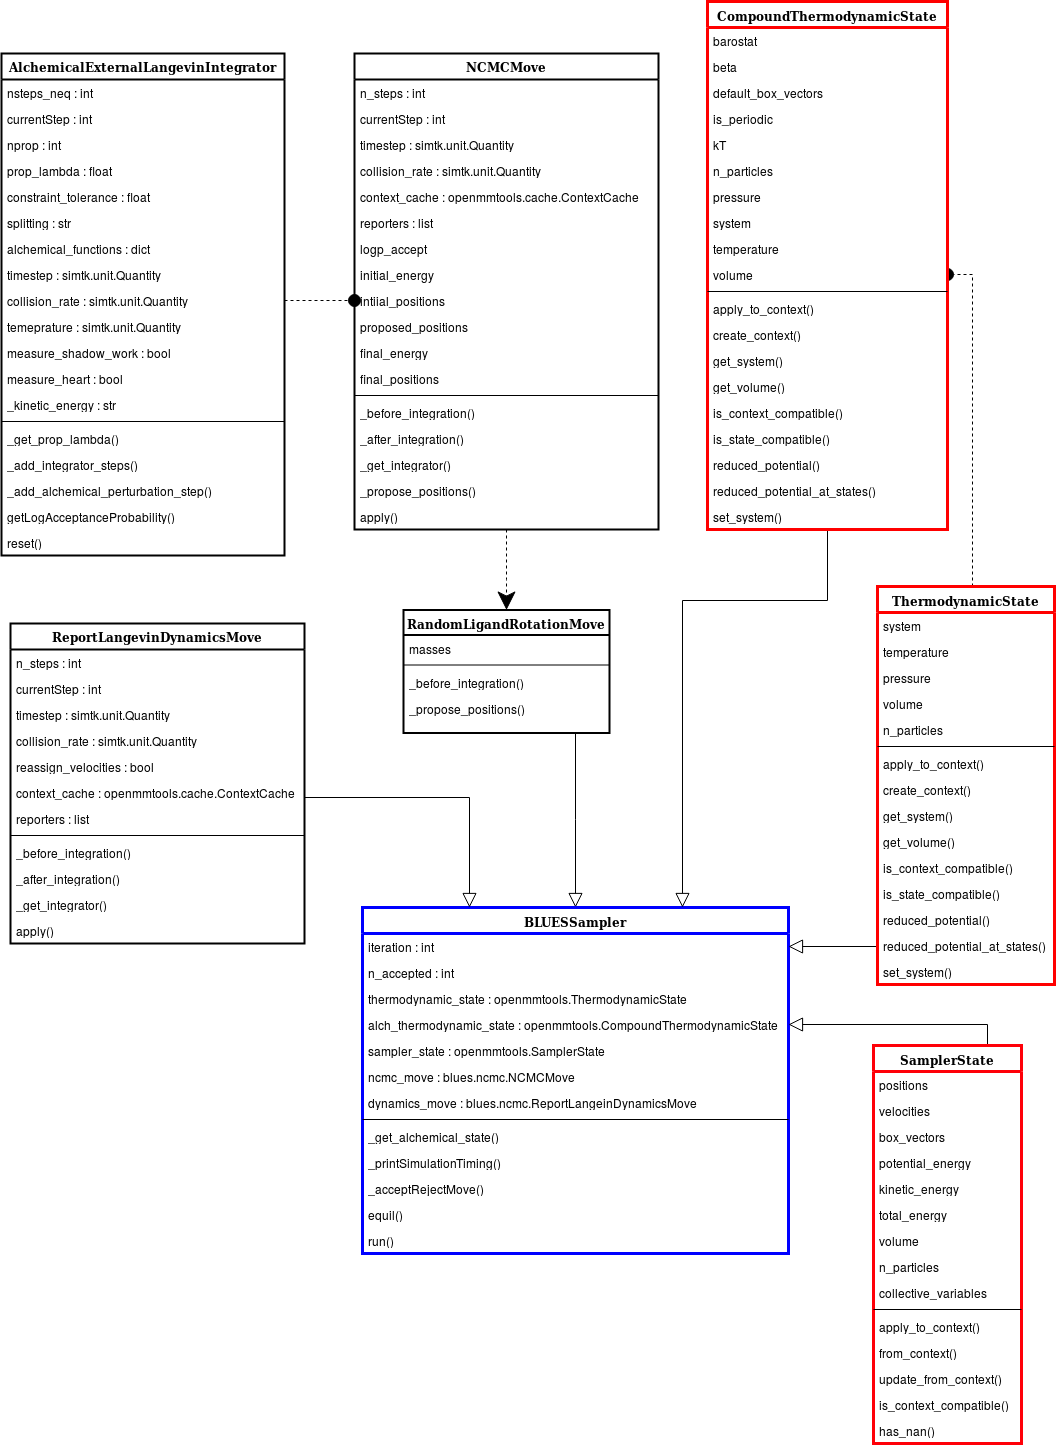
\includegraphics[width=\textwidth,height=\textheight,keepaspectratio]{blues-docs/images/uml.png}
\caption[BLUES UML Diagram]{BLUES UML Diagram provides an overview of the class objects involved in the BLUES protocol. Each class object is detailed with the attributes and methods belonging to each object.}
\label{fig:blues-uml}
\end{figure}

\hypertarget{openmmtools-objects}{%
\subsection{OpenMMTools Objects}\label{openmmtools-objects}}

Highlighted in red are 3 objects that we use from the
\texttt{openmmtools} library. They are the \textbf{ThermodynamicState},
\textbf{CompoundThermodynamicState}, and \textbf{SamplerState} objects.
For more details of each class, please see the official
\href{https://openmmtools.readthedocs.io/en/0.18.1/states.html\#thermodynamic-and-sampler-states}{openmmtools
documentation}.

Briefly, the \textbf{ThermodynamicState} class represents the portion of the state of an \texttt{openmm.Context} that does not change with integration (i.e. particles, temperature, or pressure).
The \textbf{CompoundThermodynamicState} class is essentially the same as the \textbf{ThermodynamicState} class except in this package, it is used for the handling the \texttt{openmmtools.alchemy.AlchemicalState} object.
Thus, in order to create the \textbf{CompoundThermodynamicState}, one needs to first create the plain \textbf{ThermodynamicState} object first. 
If a \textbf{CompoundThermodynamicState} object is not provided to the \texttt{blues.ncmc.BLUESSampler} class, one is created using the default parameters from the given \textbf{ThermodynamicState}. 
Lastly, the \textbf{SamplerState} class represents the state of an \texttt{openmm.Context} which does change with integration (i.e positions, velocities, and box\_vectors). 
Within the context of this package, the \textbf{SamplerState} is used to sync information between the MD and NCMC simulations.

\hypertarget{integrators-and-moves}{%
\subsection{Integrators and Moves}\label{integrators-and-moves}}

\subsubsection{Integrators} 
Integrators are the lowest level openmm objects this package interacts with, where each integrator is tied to an \texttt{openmm.Context} that it advances. 
Each integrator is generated by using the embedded function \texttt{_get_integrator()} function within each move class.
The integrators will control whether we are carrying out the Non-equilibrium Candidate Monte Carlo (NCMC) or Molecular Dynamics (MD) simulation.

Every move class has 3 hidden methods: \texttt{_get_integrator()} for generating the integrator of each move class, \texttt{_before_integration()} for performing any necessary setup before integration, and \texttt{after_integration} for performing any cleanup or data collection after integration. 
Every move class also contains the \texttt{apply()} method which carries out calls to the 3 hidden methods and stepping with the integrator.

In this package, we provide the move class \texttt{blues.ncmc.ReportLangevinDynamicsMove} to execute the MD simulation.
As the name suggests, this will carry forward the MD simulation using Langevin dynamics, by generating an \texttt{openmm.LangevinIntegrator}.
This class is essentially the same as the \texttt{openmmtools.LangevinDynamicsMove} but with modifications to the \texttt{apply()} method which allows storing simulation data for the MD simulation.

For running the NCMC simulation, we provide a custom integrator \texttt{blues.integrator.AlchemicalExternalLangevinIntegrator}. 
This integrator is generated in every move which inherits from the base class \texttt{blues.ncmc.NCMCMove}.
Every class which inherits from the base move class must override the \texttt{_propose_positions()} method.
If necessary, one can override the \texttt{_before_integration()} and \texttt{_after_integration()} methods for any necessary setup and cleanup.
Again, these hidden methods will be called when a call is made to the \texttt{apply()} method from the move class.

\subsubsection{Moves}
In order to implement custom NCMC moves, inherit from the base class and override the \texttt{_propose_positions()} method. 
This method is expected to take in a positions array of the atoms to be modified and returns the proposed positions.
In pseudo-code, it would look something like:

\begin{minted}[breaklines]{python}
from blues.ncmc import NCMCMove
class CustomNCMCMove(NCMCMove):
   def _propose_positions(positions):
       """Add 1 nanometer displacement vector."""
       positions_unit = positions.unit
       unitless_displacement = 1.0 / positions_unit
       displacement_vector = unit.Quantity(np.random.randn(3) * unitless_displacement_sigma, positions_unit)
       proposed_positions = positions + displacement_vector
       return proposed_positions
\end{minted}

In this package, we provide the \texttt{blues.ncmc.RandomLigandRotationMove} in order to propose a random ligand rotation about the center of mass.
This class overrides the \texttt{_before_integration()} method for obtaining the masses of the ligand and overrides the \texttt{_propose_positions()} function for generating the rotated coordinates. Updating the context with the rotated coordinates is handled when the \texttt{apply()} method is called in the move class. 
Code snippet of the class is shown below:

\begin{minted}[breaklines]{python}
from blues.ncmc import RandomLigandRotationMove
class RandomLigandRotationMove(NCMCMove):
  def _before_integration(self, context, thermodynamic_state):
     """Obtain the masses of the ligand before integration."""
     super(RandomLigandRotationMove, self)._before_integration(context, thermodynamic_state)
     masses, totalmass = utils.getMasses(self.atom_subset, thermodynamic_state.topology)
     self.masses = masses
  def _propose_positions(self, positions):
      # Calculate the center of mass
      center_of_mass = utils.getCenterOfMass(positions, self.masses)
      reduced_pos = positions - center_of_mass
      # Define random rotational move on the ligand
      rand_quat = mdtraj.utils.uniform_quaternion(size=None)
      rand_rotation_matrix = mdtraj.utils.rotation_matrix_from_quaternion(rand_quat)
      # multiply lig coordinates by rot matrix and add back COM translation from origin
      proposed_positions = numpy.dot(reduced_pos, rand_rotation_matrix) * positions.unit + center_of_mass

      return proposed_positions
\end{minted}

Since BLUES (v0.2.5) the API has been re-written to be more compatible with the \texttt{openmmtools} API.
This means one can turn a regular \href{https://openmmtools.readthedocs.io/en/0.18.1/mcmc.html\#mcmc-move-types}{Markov Chain Monte Carlo (MCMC)} move from the \texttt{openmmtools} library into an NCMC move to be used in this package. In this case, one simply needs to make use of dual inheritance, using the \texttt{blues.ncmc.NCMCMove} that we provide and override the \texttt{_get_integrator()} method to generate the NCMC integrator we
provide, i.e. \texttt{blues.integrator.AlchemicalExternalLangevinIntegrator}.
When using dual inheritance, it is important that you first inherit the desired MCMC move and then the \texttt{blues.ncmc.NCMCMove} class.
For example, if we wanted to take the\texttt{openmmtools.mcmc.MCDisplacementMove} class and turn it into an NCMC move, it would look like:

\begin{minted}[breaklines]{python}
from blues.ncmc import NCMCMove
from openmmtools.mcmc import MCDisplacementMove
class NCMCDisplacementMove(MCDisplacementMove, NCMCMove):
   def _get_integrator(self, thermodynamic_state):
       return NCMCMove._get_integrator(self,thermodynamic_state)

\end{minted}

\hypertarget{bluessampler}{%
\subsection{BLUESSampler}\label{bluessampler}}

The \texttt{blues.ncmc.BLUESSampler} object ties together all the previously mentioned state objects and the two move classes for running the NCMC+MD simulation.
Details of the parameters for this class are listed in the \texttt{module_doc} documentation.
For a more detailed example of it's usage see the \texttt{usage} documentation.
To be explicit, the input parameters refer to the objects below:

\begin{itemize}
\tightlist
\item
  \textbf{thermodynamic\_state} :
  \texttt{openmmtools.states.ThermodynamicState}
\item
  \textbf{alch\_thermodynamic\_state} :
  \texttt{openmmtools.states.CompoundThermodynamicState}
\item
  \textbf{sampler\_state} : \texttt{openmmtools.states.SamplerState}
\item
  \textbf{dynamics\_move} :
  \texttt{blues.ncmc.ReportLangevinDynamicsMove}
\item
  \textbf{ncmc\_move} : \texttt{blues.ncmc.RandomLigandRotationMove}
\item
  \textbf{topology} : \texttt{openmm.Topology}
\end{itemize}

When the \texttt{run()} method in the \texttt{blues.ncmc.BLUESSampler} is called the following takes place:
\begin{itemize}
\item
  \begin{description}
  \item[Initialization:] 
  \begin{itemize}
  \tightlist
  \item
    \texttt{_print_host_info()} : Information print out of host
  \item
    \texttt{_printSimulationTiming()} : Calculation of total number of steps
  \item
    \texttt{equil()} : Equilibration
  \end{itemize}
  \end{description}
\item
  \begin{description}
  \item[BLUES iterations:]
  \begin{itemize}
  \tightlist
  \item
    \texttt{ncmc_move.apply()} : NCMC simulation
  \item
    \texttt{_acceptRejectMove()} : Metropolization
  \item
    \texttt{dynamics_move.apply()} : MD Simulation
  \end{itemize}
  \end{description}
\end{itemize}

A code snippet of the \texttt{run()} method is shown below:

\begin{minted}[breaklines]{python}
def run(self, n_iterations=1):
   context, integrator = cache.global_context_cache.get_context(self.thermodynamic_state)
   utils.print_host_info(context)
   self._printSimulationTiming(n_iterations)
   if self.iteration == 0:
       self.equil(1)

   self.iteration = 0
   for iteration in range(n_iterations):
       self.ncmc_move.apply(self.alch_thermodynamic_state, self.sampler_state)

       self._acceptRejectMove()

       self.dynamics_move.apply(self.thermodynamic_state, self.sampler_state)

       self.iteration += 1
\end{minted}

\hypertarget{initialization}{%
\subsubsection{Initialization}\label{initialization}}

The first thing that occurs when \texttt{run()} is called is the initialization stage.
During this stage, a call is made to \texttt{utils.print_host_info()} and the \texttt{_printSimulationTiming()} method which will print out some information about the host machine , the total number of force evaluations, and simulation time. 
The output will look something like below:

\begin{verbatim}
OpenMM(7.3.1.dev-4a269c0) Context generated for CUDA platform
system = Linux
node = titanpascal
release = 4.15.0-50-generic
version = #54~16.04.1-Ubuntu SMP Wed May 8 15:55:19 UTC 2019
machine = x86_64
processor = x86_64
DeviceIndex = 0
DeviceName = TITAN Xp
UseBlockingSync = true
Precision = single
UseCpuPme = false
CudaCompiler = /usr/local/cuda-9.2/bin/nvcc
TempDirectory = /tmp
CudaHostCompiler =
DisablePmeStream = false
DeterministicForces = false

Total BLUES Simulation Time = 4.0 ps (0.04 ps/Iter)
Total Force Evaluations = 4000
Total NCMC time = 2.0 ps (0.02 ps/iter)
Total MD time = 2.0 ps (0.02 ps/iter)
\end{verbatim}

In the \texttt{blues.ncmc.BLUESSampler} class, there is an \texttt{equil()} method which lets you run iterations of just the MD simulation in order to equilibrate your system before running the NCMC+MD hybrid simulation. 
An equilibration iteration, in this case is controlled by the given attribute \emph{n\_steps} from the \emph{dynamics\_move} class.
For example, if I create a \texttt{blues.ncmc.ReportLangevinDynamicsMove} class with \emph{n\_steps=20} and call the \texttt{blues.ncmc.BLUESSampler.equil(n_iterations=100)}, this will run \emph{(n\_steps x n\_iterations)} or 2000 steps of MD or 2 picoseconds of MD simulation time.
When the \texttt{run()} method is called without a prior call to the \texttt{equil()} method, the class will always run 1 iteration of equilibration in order to set the initial conditions in the MD simulation.
This is required prior to running the NCMC simulation.

\hypertarget{blues-iterations}{%
\subsubsection{BLUES Iterations}\label{blues-iterations}}

\subsubsection{NCMC Simulation}

After at least 1 iteration of equilibration, the \texttt{blues.ncmc.BLUESSampler} class will then proceed forward with running iterations of the NCMC+MD hybrid simulation.
It will first run the NCMC simulation by calling the \texttt{apply()} method on the \textbf{ncmc\_move} class or, for sake of this example, the \texttt{blues.ncmc.RandomLigandRotationMove} class.
The \texttt{apply()} method for the \textbf{ncmc\_move} will take in the \textbf{alch\_thermodynamic\_state} parameter or specifically the \texttt{openmmtools.states.CompoundThermodynamicState} object.

A code snippet of the \texttt{ncmc_move.apply()} method is shown below:

\begin{minted}[breaklines]{python}
def apply(self, thermodynamic_state, sampler_state):
   if self.context_cache is None:
       context_cache = cache.global_context_cache
   else:
       context_cache = self.context_cache
   integrator = self._get_integrator(thermodynamic_state)
   context, integrator = context_cache.get_context(thermodynamic_state, integrator)
   sampler_state.apply_to_context(context, ignore_velocities=False)
   self._before_integration(context, thermodynamic_state)
   try:
       endStep = self.currentStep + self.n_steps
       while self.currentStep < endStep:
           alch_lambda = integrator.getGlobalVariableByName('lambda')
           if alch_lambda == 0.5:
               sampler_state.update_from_context(context)
               proposed_positions = self._propose_positions(sampler_state.positions[self.atom_subset])
               sampler_state.positions[self.atom_subset] = proposed_positions
               sampler_state.apply_to_context(context, ignore_velocities=True)

           nextSteps = endStep - self.currentStep
           stepsToGo = nextSteps
           while stepsToGo > 10:
               integrator.step(10)
               stepsToGo -= 10
           integrator.step(stepsToGo)
           self.currentStep += nextSteps
   except Exception as e:
       print(e)
   else:
       context_state = context.getState(
           getPositions=True,
           getVelocities=True,
           getEnergy=True,
           enforcePeriodicBox=thermodynamic_state.is_periodic)

       self._after_integration(context, thermodynamic_state)
       sampler_state.update_from_context(
           context_state, ignore_positions=False, ignore_velocities=False, ignore_collective_variables=True)
\end{minted}

When the \texttt{apply()} method on \textbf{ncmc\_move} is called, it will first generate the \texttt{blues.integrators.AlchemicalExternalLangevinIntegrator} by calling the \texttt{_get_integrator()} method inherent to the move class. 
Then, it will create (or fetch from the \textbf{context\_cache}) a corresponding \texttt{openmm.Context} given the \textbf{alch\_thermodynamic\_state}.
Next, the \textbf{sampler\_state} which contains the last state of the MD simulation is synced to the
newly created context from the corresponding \textbf{alch\_thermodynamic\_state}.
Particularly, the context will be updated with the \emph{box\_vectors}, \emph{positions}, and
\emph{velocities} from the last state of the MD simulation.

Just prior to integration, a call is made to the \texttt{_before_integration()} method in order to store the initial \emph{energies}, \emph{positions}, \emph{box\_vectors} and the \emph{masses} of the ligand to be rotated.
Then, we actually step with the integrator where we perform the ligand rotation when \emph{lambda} has reached the half-way point or \emph{lambda=0.5}, continuing integration until we have completed the \emph{n\_steps}.
After the integration steps have been completed, a call is made to the \texttt{after_integration} method to store the final \emph{energies}, \emph{positions}, and \emph{box\_vectors}.
Lastly, the \textbf{sampler\_state} is updated from the final state of the context.


\subsubsection{Metropolization}

After advancing the NCMC simulation, a call is made to the \texttt{_acceptRejectMove()} method embedded in the \texttt{blues.ncmc.BLUESSampler} class for metropolization of the proposed move.
A code snippet of the \texttt{_acceptRejectMove()} is shown below:

\begin{minted}[breaklines]{python}
def _acceptRejectMove(self):
   integrator = self.dynamics_move._get_integrator(self.thermodynamic_state)
   context, integrator = cache.global_context_cache.get_context(self.thermodynamic_state, integrator)
   self.sampler_state.apply_to_context(context, ignore_velocities=True)
   alch_energy = self.thermodynamic_state.reduced_potential(context)

   correction_factor = (self.ncmc_move.initial_energy - self.dynamics_move.final_energy + alch_energy - self.ncmc_move.final_energy)
   logp_accept = self.ncmc_move.logp_accept
   randnum = numpy.log(numpy.random.random())

   logp_accept = logp_accept + correction_factor
   if (not numpy.isnan(logp_accept) and logp_accept > randnum):
       self.n_accepted += 1
   else:
       self.accept = False
       self.sampler_state.positions = self.ncmc_move.initial_positions
       self.sampler_state.box_vectors = self.ncmc_move.initial_box_vectors
\end{minted}

Here, is we compute a correction term for switching between the MD and NCMC integrators and factor this in with natural log of the acceptance probability (\textbf{logp\_accept}).
Then, a random number is generated in which: the move is accepted if the random number is less than the \textbf{logp\_accept} or rejected if greater.
When the move is rejected, we set the \emph{positions} and \emph{box\_vectors} on the \textbf{sampler\_state} to the initial positions and box\_vectors from the NCMC simulation.
If the move is accepted, nothing on the \textbf{sampler\_state} is changed so that the following MD simulation will contain the final state of the NCMC simulation.

\subsubsection{MD Simulation}
After metropolization of the previously proposed move, a call is made to the \texttt{apply()} method on the given \textbf{dynamics\_move} object.
In this example, this would refer to the \texttt{blues.ncmc.ReportLangevinDynamicsMove} class to run the MD simulation.
A code snippet of the \mintinline{python}{dynamics_move.apply()} method is shown below:

\begin{minted}[breaklines, autogobble]{python}
def apply(self, thermodynamic_state, sampler_state):
   if self.context_cache is None:
       context_cache = cache.global_context_cache
   else:
       context_cache = self.context_cache

   integrator = self._get_integrator(thermodynamic_state)
   context, integrator = context_cache.get_context(thermodynamic_state, integrator)
   thermodynamic_state.apply_to_context(context)

   sampler_state.apply_to_context(context, ignore_velocities=self.reassign_velocities)
   if self.reassign_velocities:
       context.setVelocitiesToTemperature(thermodynamic_state.temperature)

   self._before_integration(context, thermodynamic_state)
   try:
       endStep = self.currentStep + self.n_steps
       while self.currentStep < endStep:
           nextSteps = endStep - self.currentStep
           stepsToGo = nextSteps
           while stepsToGo > 10:
               integrator.step(10)
               stepsToGo -= 10
           integrator.step(stepsToGo)
           self.currentStep += nextSteps

   except Exception as e:
       print(e)

   else:
       context_state = context.getState(
           getPositions=True,
           getVelocities=True,
           getEnergy=True,
           enforcePeriodicBox=thermodynamic_state.is_periodic)
       self._after_integration(context, thermodynamic_state)
       sampler_state.update_from_context(
           context_state, ignore_positions=False, ignore_velocities=False, ignore_collective_variables=True)

\end{minted}

When the \texttt{apply()} method is called, a very similar procedure to the NCMC simulation occurs. 
The first thing that happens is to generate the integrator through a call to \texttt{_get_integrator()}, where in this given class, it will generate an \texttt{openmm.LangevinIntegrator} given the \textbf{thermodynamic\_state} parameter.
Then, it will create (or fetch from the \textbf{context\_cache}) a corresponding \texttt{openmm.Context} given the \textbf{thermodynamic\_state}.
Next, the \textbf{sampler\_state}, which contains the last state of the NCMC simulation if the previous move was accepted or the initial state of the NCMC simulation if the move was rejected, is used to update \emph{box\_vectors} and \emph{positions} in the newly created \texttt{openmm.Context}. 
In this case, we reassign the \emph{velocities} in the MD simulation in order to preserve detailed balance.

Following, a call is made to \texttt{_before_integration()} to store the intial \emph{positions}, \emph{box\_vectors} and \emph{energies} and then we carry forward with the integration for \emph{n\_steps}.
After the integration steps have been completed, a call is made to the \texttt{after_integration} method to store the final \emph{energies} and \emph{positions}.
Lastly, the \textbf{sampler\_state} object is updated from the final state of the MD simulation context.

This completes 1 iteration of the BLUES cycle. 
Here, the\textbf{sampler\_state} is then used to sync the final state of the MD simulation (i.e. \emph{box\_vectors}, \emph{positions}, and \emph{velocities}) from the previous iteration to the NCMC simulation of the next iteration. 
Then, we repeat the cycle of \textbf{NCMC-\textgreater{} Metropolization -\textgreater{} MD} for the given number of iterations.
    \section{Conclusion}
On the BLUES project, my primary contribution was to incorporate the best practices in software development such as: (1) version control, (2) testing and code coverage, (3) continuous integration, (4) automated build systems, (5) standardized code style, and (6) documentation.
Incorporation of these design principles ensure long-term reliability, reproducibility, and viability in the code and go towards helping others continue future work and extensions on the BLUES project.
The BLUES software package is available on Github with 80\% of the code base tested, continually integrated with Travis-CI, and the documentation available on ReadTheDocks. 
I have written the code to adhere to the PEP8 format \cite{pep8} and the documentation follows the numpydoc \cite{numpydoc} format.

Furthermore, by designing the BLUES toolkit to be as modular as possible, this has enabled easy implementation of new NCMC move types to enhance sampling beyond simple ligand rotations.
Recent work in the Mobley lab has included implementation of NCMC moves such as: sidechain rotations \cite{burley2019enhancing} for enhancing protein motions, rotations in ligand torsional angles, and `water-hopping' for enhanced sampling of water motions.
These recent studies utilize the same code base as seen in our studies with simple random ligand rotations, but have simply replaced the ligand rotation function with these alternative moves.
Since version 0.2.5, the BLUES code has been re-designed to be compatibility with other software packages like `openmmtools' \cite{openmmtools} to allow simple conversion of their Markov-chain Monte Carlo moves into NCMC moves, to be used in the NCMC+MD hybrid simulation framework that the BLUES toolkit provides.

Incorporation of these design principles ensure long-term reliability, reproducibility, and viability in the code and go towards helping others continue future work and extensions on the BLUES project. 
\chapter{Identifying the binding modes of a novel RNA nucleoside analog} \label{UCK2}

\small{Authors: Nathan M. Lim, Sarah Nainar, Bonnie Cuthbert, David L. Mobley, Celia Goulding, Robert Spitale}\\
\emph{Part of: `An Optimized Chemical-Genetic Method for Cell-Specific Metabolic Labeling of RNA' \cite{uck2paper}}\\
\emph{Submitted to Journal of Nature Methods}

\section{Introduction}
The Spitale Lab at UCI had synthesized several RNA nucleoside analogs for the purpose to developing a method for cell-specific labeling of RNA.
In this study, the Spitale group was interested in understanding how their novel RNA nucleoside analogs would bind to the protein uridine-cytidine kinase 2, which was found to allow incorporation of their RNA nucleoside analogs into nascent RNA strands.
Here, I demonstrate the use of docking and molecular dynamics (MD) simulations for validating their hypothesis of their nucleoside analogs binding in the same mode as the endogenous ligand, cytidine, as well as uncovering a novel binding mode, representative of the post-catalytic state.
These predictions of the binding modes were then later validated by x-ray crystallography.

\section{Computational Methods}
The starting structure used for the molecular dynamics (MD) simulations was taken from the crystal structure of human uridine-cytidine kinase 2 complex with the cytidine substrate (PDBID: 1UEJ) \cite{suzuki2004structural}.
In this study four different MD simulations were carried out, using two different binding modes for each of the respective ligands 2AZU and 2AZC.
Here, we differentiate between the two binding modes by the orientation of the ribose moiety on the molecule. 
The "canonical" binding mode refers to the pose in which the azide (substituted on the 2' position) is pointed inwards into the binding site, see Figure \ref{fig:2AZC-xtal}.
We refer to this as the canonical binding mode as this pose is similar to the pose found in the crystal structure with the bound cytidine substrate (PDBID: 1UEJ).
The "flipped" binding mode refer to the pose in which the azide is pointed outwards from the binding site, see Figure \ref{fig:2AZU-xtal}.

A total of 500ns of MD simulation time was conducted for each binding mode by running 5 simulations each, where each copy of the simulation began from the same protein structure.
The metastable binding modes sampled during our MD simulations were defined by constructing a Markov State Model (MSM) from our pool of MD simulation data and clustering with perron-cluster cluster analysis (PCCA).
We then compared these metastable binding modes with x-ray crystal structures for 2AZU and 2AZC by computing the root-mean-square deviation (RMSD) between the ligand heavy atoms.
We would like to note that the x-ray crystal structures of 2AZU and 2AZC were not used for setup or seen prior to conducting our MD simulations.
Our simulation results, along with the x-ray crystal structures, support the hypothesis that the ligands must adopt the "flipped" binding mode for catalytic turnover.

\subsection{MD simulation parameters}
All simulations in this study were conducted using OpenMM v7.1.1 \cite{openmm} at T=300K and P=1atm.
Here, we use timesteps of 4fs by employing the hydrogen mass repartitioning (HMR) scheme \cite{hmr}. 
This scheme allows us to take larger timesteps by slowing down the fastest motions (i.e. hydrogen bond stretching) in our MD simulations.
The HMR scheme constraints the bond length between hydrogens and their connected heavy atoms and reallocates mass from the connected heavy atom to the hydrogens.
The protein-ligand systems were placed in a periodic box with explicit TIP3P water molecules using a 10A solvent padding distance and counter ions (NaCl) were added using a concentration of 150mM.
A 10A cut-off distance was used for the particle-mesh Ewald method for computing long-range (e.g. electrostatic) interactions.
Protein atoms were parameterized using the `amber99sbildn' forcefields \cite{amber99sbildn} and the ligands were parameterized using GAFF2 \cite{ambergaff} in which atomic charges were assigned using the AM1-BCC charge model \cite{am1bcc}.

\subsection{Protein preparation}
To prepare the protein system (PDBID: 1UEJ) for MD simulations, we used PDBFixer \cite{pdbfixer} to model in missing residues, add missing hydrogen atoms, and solvate our system.
Sidechains were protonated in accordance with the pH=8.0 environment of the enzyme assay experiments \cite{doi:10.1021/bi102054n} and as described in other computational studies \cite{tanaka2016molecular}.
With the cytidine molecule bound, we energy minimized the protein-ligand complex for a maximum of 30,000 steps and followed with an equilibration protocol as follows.
The equilibration protocol occurs in four 10 ps stages, whereby a progressively declining restraining force was used to help the protein-ligand system gradually relax.
First, we apply a restraining force of 2.0 to the heavy atoms of the protein-ligand complex, simulate for 10ps using constant volume (NVT), and follow-up with 10ps at constant pressure (NPT).
Next, we decrease the restraining force to 0.5 and then conduct an NPT simulation for 10ps.
Last, we use a 0.1 restraining force on the alpha-carbons (protein backbone) and the ligand heavy atoms and then NPT simulate for 10ps.

\subsection{Docking}
After equilibration of the UCK2-cytidine complex, we applied HYBRID docking \cite{mcgann2012fred} to dock our nucleoside analogs (2AZU and 2AZC) into the binding site.
HYBRID differs from the standard docking approach such that the software will use the co-crystallized ligand as a reference point and attempt to fit the nucleoside analogs within the binding site by overlaying the docked ligands with the crystallographic ligand.
From HYBRID docking, we generated up to 50 different conformers for each nucleoside analog and then followed the same equilibration protocol described previously.
After equilibration, we found that the conformers tended to converge into two groups: 1 conformer which resembled the "canonical" binding mode and another which had the ribose moiety "flipped".
We then selected 1 conformer from each representative group and carried these forward for our production NPT 100ns MD simulations (no restraints).

\subsection{Analysis}
For each nuceloside analog (2AZC and 2AZU), we ran five 100ns MD simulations for each of the two binding modes (canonical and flipped).
They are denoted as $2AZC_{canc}$, $2AZC_{flip}$, $2AZU_{canc}$, and $2AZU_{flip}$.
Collectively, over the course of the 100ns of simulation time, the root-mean-square deviation (RMSD) for the ligand atoms began to stabilize after 25ns.
Thus, we discard trajectory frames from 0-25ns as additional equilibration time and only perform further analysis from the 25ns-100ns time frame Fig.\ref{fig:2AZC_canc-rmsd_trim}.
The RMSD is calculated by:
\begin{equation}
    RMSD = \sqrt{ \frac{1}{n} \sum^{n}_{i=1}{d_{i}^{2}}}
\end{equation}
where $d_{i}$ represents the distance between the $n$ atom pairs.
For construction of our Markov State models (MSM), we use the PyEMMA v2.5.5 \cite{scherer2015pyemma} toolkit.
For residue contact analyses we use the MDTraj v1.9.1 \cite{mcgibbon2015mdtraj} and VMD v1.9.3 \cite{humphrey1996vmd} toolkits.

\subsubsection*{Defining the metastable binding modes}

\begin{figure}[!ht]
\centering
\begin{subfigure}{.5\textwidth}
  \centering
  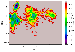
\includegraphics[width=.9\linewidth]{chapter4/2AZC_canc/2AZC_canc-tica}
  \caption{$2AZC_{canc}-TICA$}
  \label{fig:2AZC_canc-tica}
\end{subfigure}%
\begin{subfigure}{.5\textwidth}
  \centering
  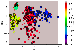
\includegraphics[width=.9\linewidth]{chapter4/2AZC_canc/2AZC_canc-pcca}
  \caption{$2AZC_{canc}-PCCA$}
  \label{fig:2AZC_canc-pcca}
\end{subfigure}
\caption[PCCA Analysis of $2AZC_{canc}$]{PCCA clustering in TICA space from simulations of $2AZC_{canc}$. MD simulations for $2AZC_{canc}$ show sampling of 4 different binding modes (red, yellow, blue, green), where the primary binding mode is indicated in red.}
\label{fig:2AZC_canc-cluster}
\end{figure}

In order to define our metastable binding modes and visualize their structures, we construct a Markov State model (MSM) \cite{prinz2011markov} from our five separate MD simulations.
Our features for constructing the MSMs consists of the distance between the closest heavy atoms on the ligand and the following 9 residues: ASP62, PHE83, ASP84, TYR112, PHE114, HIS117, ILE137, ARG166, and ARG176.
These residues were selected as they have been noted in the literature to play important roles in binding \cite{tanaka2016molecular}.
From this feature space, we apply the time-lagged independent component analysis (TICA) method using a lagtime of 1ns.
TICA transforms our 9 dimensional feature space to a new set of reaction coordinates which maximizes the autocorrelation of the transformed coordinates \cite{perez2013identification}.
In other words, TICA allows us to extract the slow order parameters and project them into a lower dimensional space; here, we use the first two TICA coordinates (Fig. \ref{fig:2AZC_canc-tica}).
Then, we apply k-means clustering to discretize our trajectory frames into discrete microstate and project them into TICA space (denoted by individual Xs).
Following, we use perron-cluster cluster analysis (PCCA) \cite{roblitz2013fuzzy} to assign each microstate to a metastable macrostate (denoted by color in Fig.\ref{fig:2AZC_canc-pcca}).
From each of our assigned macrostates, we randomly sample 100 frames and then visualize the frame which minimizes the RMSD to the crystallographic ligand.

\subsubsection*{Distance to key residues}
Using the `$compute\_contacts$' tool from MDTraj, we compute the distance between the closest heavy atoms in the ligand and 4 residues: ASP62, TYR112, HIS117 and ARG176 (Fig.\ref{fig:contact-distance}).
These residues were chosen in particular as ASP62 is known to be the catalytic residue, while TYR112, HIS117, and ARG176 are believed to play a key role in substrate specificity between uridine and cytidine as they have been found to bind to the nucleobase moiety \cite{tanaka2016molecular}.
Here, we calculate the frequency in which the distance between the ligand and the residues are less than or equal to 3.0A, which we define as the minimum distance needed to form an interactive bond.

\subsubsection*{Hydrogen Bond Contacts}

We compute the frequency of hydrogen bond contacts between the ligands and surrounding residues using the HBonds plugin v1.2 in VMD 1.9.3 \cite{humphrey1996vmd}, shown in Figure \ref{fig:HBonds}.
The criterion used for defining formation of a hydrogen bond is that the cutoff distance between a hydrogen bond donor and acceptor must be less than 3.0\angstrom and the angle is less than 20 degrees.
Each colored bar corresponds to the hydrogen bond frequency from an individual MD simulation.

\subsubsection*{Comparisons to X-ray Crystal Structures}
Here, we compared our metastable binding modes from our MD simulations against each subunit found in the experimental x-ray crystal structures and list the values against the subunit which minimizes the computed RMSD.
To compare the metastable binding modes from our MD simulations with experimental x-ray crystal structures, we first align the two structures using the protein backbone.
Particularly, we align by the protein backbone using residues 19 to 229 but exclude residues 48 to 52 as these were missing in the x-ray crystal structures.
Once aligned by the protein backbone, we then compute the RMSD between crystallized ligand and the matching ligand heavy atoms from our defined metastable binding modes.

\section{Results}

\subsection{Binding Mode Stability}

\begin{figure}[!ht]
\centering
   \begin{subfigure}{.45\textwidth}
     \centering
     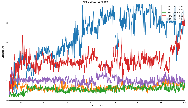
\includegraphics[width=.95\linewidth]{chapter4/2AZC_canc/2AZC_canc-rmsd-trim}
     \caption{$2AZC_{canc}-rmsd_trim$}
     \label{fig:2AZC_canc-rmsd_trim}
   \end{subfigure}
   \begin{subfigure}{.45\textwidth}
     \centering
     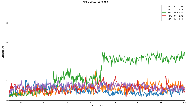
\includegraphics[width=.95\linewidth]{chapter4/2AZU_canc/2AZU_canc-rmsd-trim}
     \caption{$2AZU_{canc}-rmsd_trim$}
     \label{fig:2AZU_canc-rmsd_trim}
   \end{subfigure}
   \\
   \begin{subfigure}{.45\textwidth}
     \centering
     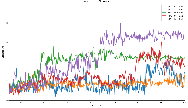
\includegraphics[width=.95\linewidth]{chapter4/2AZC_flip/2AZC_flip-rmsd-trim}
     \caption{$2AZC_{flip}-rmsd_trim$}
     \label{fig:2AZC_flip-rmsd_trim}
   \end{subfigure}
    \begin{subfigure}{.45\textwidth}
     \centering
     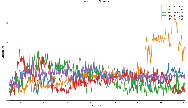
\includegraphics[width=.95\linewidth]{chapter4/2AZU_flip/2AZU_flip-rmsd-trim}
     \caption{$2AZU_{flip}-rmsd_trim$}
     \label{fig:2AZU_flip-rmsd_trim}
   \end{subfigure}
\caption[RMSD for 2AZC and 2AZU]{RMSDs ({\AA}) for ligand heavy atoms from 25-100ns MD simulations for 2AZC and 2AZU in the cannonical or flipped binding mode. Each colored line represents the RMSD over time for each individual MD simulation.}
\label{fig:rmsd}
\end{figure}  

\begin{table}[!ht]
\caption{Average RMSD ({\AA}) for ligand heavy atoms over the course of the 25-100ns MD simulations}
\label{table:rmsd}
\begin{tabular}{|l|l|l|l|l|l|l|l|}
\hline
                    & RMSD & RMSD & RMSD & RMSD & RMSD & \textbf{AVG}  & SEM           \\ \hline
\textbf{2AZC\_canc} & 6.7 & 1.3 & 1.1 & 4.1 & 2.1 & \textbf{3.1} & \textit{1.0} \\ \hline
\textbf{2AZU\_canc} & 0.9 & 1.2 & 2.9 & 1.3 & 1.4 & \textbf{1.5} & \textit{0.4} \\ \hline
\textbf{2AZC\_flip} & 1.8 & 1.7 & 4.0 & 2.6 & 4.6 & \textbf{3.0} & \textit{0.6} \\ \hline
\textbf{2AZU\_flip} & 2.4 & 3.1 & 2.4 & 2.2 & 2.6 & \textbf{2.5} & \textit{0.2} \\ \hline

\end{tabular}
\end{table}

The averages and the standard errors of the mean (SEM) for the RMSD ({\AA}) of each ligand binding mode are shown in Fig.\ref{fig:rmsd} and Table\ref{table:rmsd}.
They are $3.1 \frac{+}{-} 1.0$, $1.5 \frac{+}{-} 0.4$, $3.0 \frac{+}{-} 0.6$, and $2.5 \frac{+}{-} 0.2$ for $2AZC_{canc}$, $2AZU_{canc}$, $2AZC_{flip}$, and $2AZU_{flip}$, respectively.

Comparing the RMSD of the cannonical binding modes for 2AZC and 2AZU, we find that the 2AZU ligand to be much more stable than the 2AZC ligand.
In $\frac{2}{5}$ of our MD simulations for $2AZC_{canc}$ (Fig.\ref{fig:2AZC_canc-rmsd_trim}), the ligand comes nearly unbound after 30ns; while for $2AZU_{canc}$ (Fig. \ref{fig:2AZU_canc-rmsd_trim}) the ligand nearly unbinds in only $\frac{1}{5}$ of the simulations.
When comparing $2AZC_{flip}$ and $2AZU_{flip}$, the average RMSD suggests both are about equally stable.
However, this particular binding mode appears to show slightly more instability than the cannonical binding mode with an average RMSD of $2.6$ and $3.0$ for the $2AZC_{flip}$ and $2AZU_{flip}$, respectively.

\subsection{Distance to key residues}

In Figure \ref{fig:contact-distance}, we plot the distance between the closest ligand heavy atoms and the 4 residues: ASP62 (blue), TYR112 (orange), HIS117 (green) and ARG176 (red).
One plot from each respective binding mode was chosen from the simulation in which contact with the catalytic residue ASP62 was highest.
Additional contact distance plots from the other MD simulations can be found in the supporting information.
See Figure \ref{sup:2AZC_canc-dist} for $2AZC_{canc}$, Figure \ref{sup:2AZU_canc-dist} for $2AZU_{canc}$, Figure \ref{sup:2AZC_flip-dist} for $2AZC_{flip}$, and Figure \ref{sup:2AZU_flip-dist} for $2AZU_{flip}$.

For the canonical binding mode, we see a maximum contact frequency of 3.9\% (2AZC) and 2.5\% (2AZU) in which the ligand is $d<3.0\angstrom$ away from the catalytic residue ASP62.
Figure \ref{fig:2AZC_canc-dist} shows that the $2AZC_{canc}$ ligand in the canonical binding mode only rarely comes into contact with ASP62 but is in stable contact with HIS117 and ARG176.  
Interestingly, Figure \ref{fig:2AZU_canc-dist} illustrates that even though the $2AZU_{canc}$ ligand appears to be stably bound to the key residues (TYR112, HIS117, and ARG176) the ligand is too far away from ASP62.

In stark contrast, we see an enormous increase in contact frequency when simulating the flipped binding mode: 27.9\% for $2AZC_{flip}$ and 80.4\% for $2AZU_{flip}$.
Figure \ref{fig:2AZC_flip-dist} shows the $2AZC_{flip}$ ligand forms stable contacts with the catalytic residue ASP62 and residues TYR112/HIS117 but does not contact ARG176.
Similarly, we see the same stable contacts being formed for $2AZU_{flip}$ in Figure \ref{fig:2AZU_flip-dist}.

\begin{figure}[!ht]
\centering
   \begin{subfigure}{.45\textwidth}
     \centering
     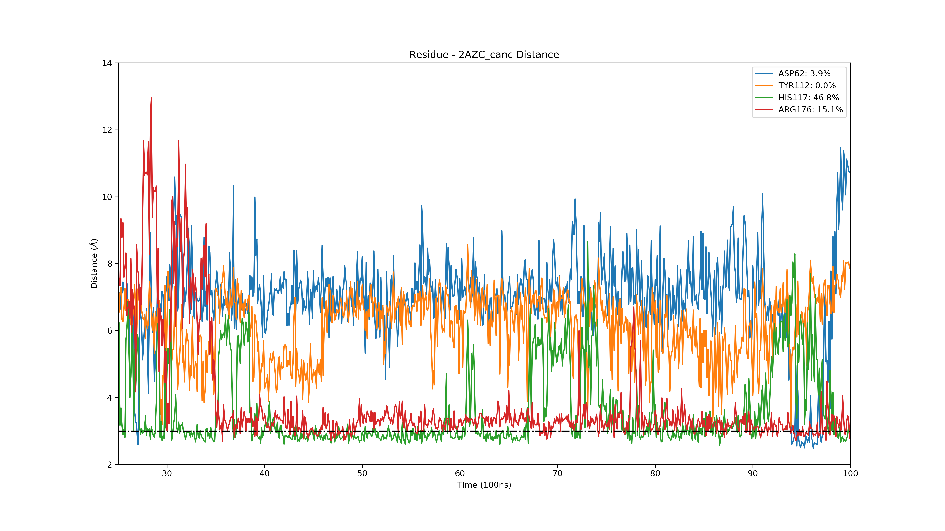
\includegraphics[width=.95\linewidth]{chapter4/2AZC_canc/2AZC_canc-dist_3.pdf}
     \caption{$2AZC_{canc}-distance$}
     \label{fig:2AZC_canc-dist}
   \end{subfigure}
   \begin{subfigure}{.45\textwidth}
     \centering
     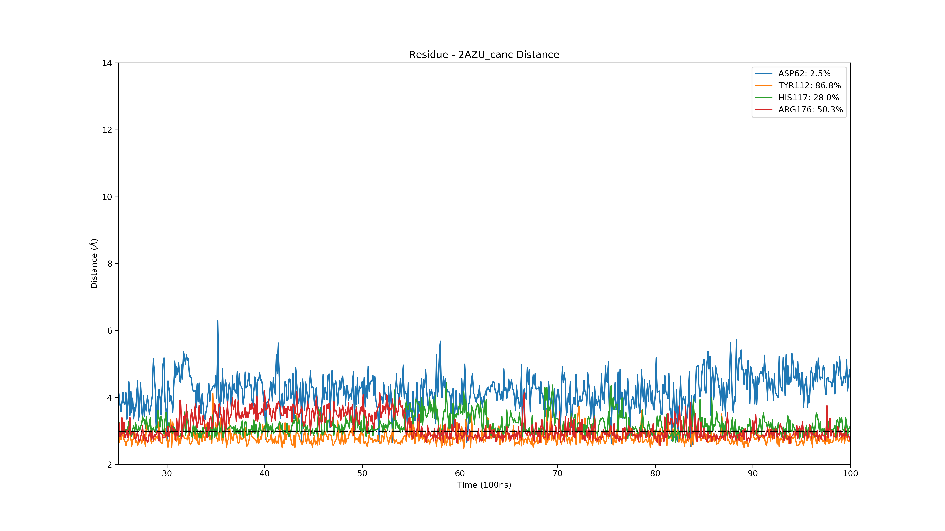
\includegraphics[width=.95\linewidth]{chapter4/2AZU_canc/2AZU_canc-dist_4.pdf}
     \caption{$2AZU_{canc}-distance$}
     \label{fig:2AZU_canc-dist}
   \end{subfigure}
   \\
   \begin{subfigure}{.45\textwidth}
     \centering
     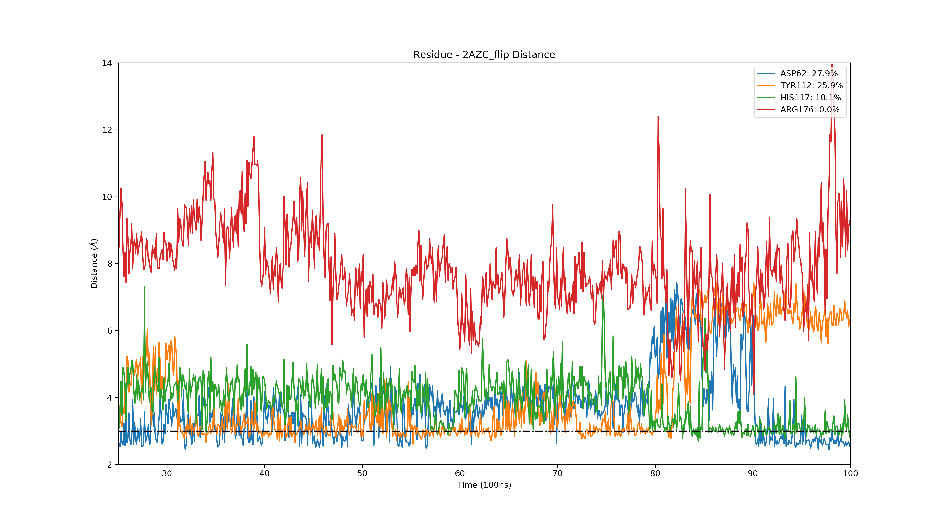
\includegraphics[width=.95\linewidth]{chapter4/2AZC_flip/2AZC_flip-dist_3.pdf}
     \caption{$2AZC_{flip}-distance$}
     \label{fig:2AZC_flip-dist}
   \end{subfigure}
    \begin{subfigure}{.45\textwidth}
     \centering
     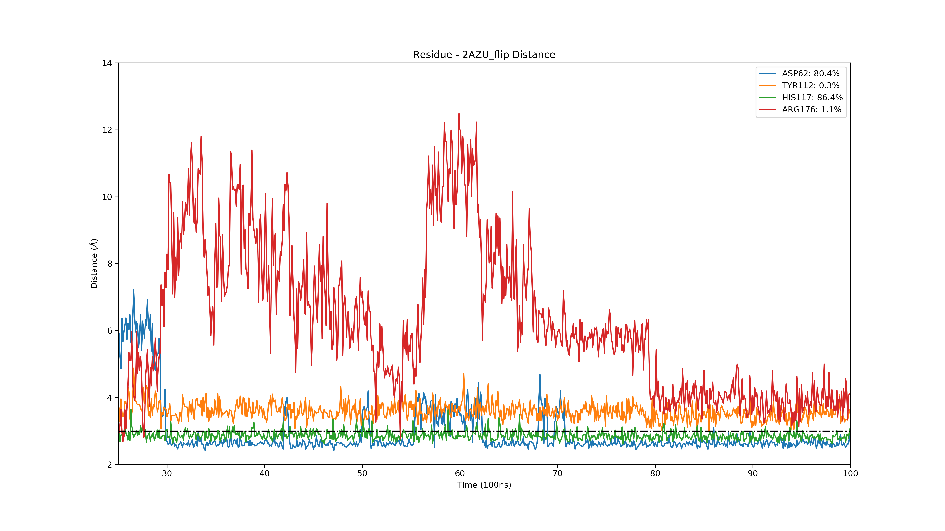
\includegraphics[width=.95\linewidth]{chapter4/2AZU_flip/2AZU_flip-dist_4.pdf}
     \caption{$2AZU_{flip}-distance$}
     \label{fig:2AZU_flip-dist}
   \end{subfigure}
\caption[Key residue distances for 2AZC/2AZU]{Distance to key residues for 2AZC and 2AZU in the cannonical and flipped binding mode from a single MD simulation. Each colored line represents the contact distance to a key residue. The distance to key residues plots from the other 4 MD simulations are shown in the supplementary information. }
\label{fig:contact-distance}
\end{figure}  

\subsection{Hydrogen Bond Contacts}

\begin{figure}[!ht]
\centering
   \begin{subfigure}{.45\textwidth}
     \centering
     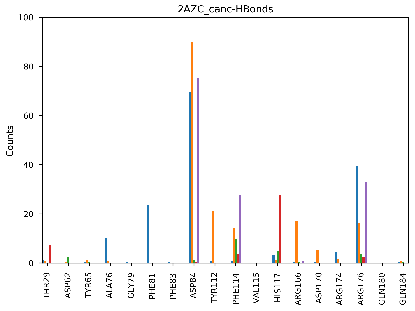
\includegraphics[width=.95\linewidth]{chapter4/2AZC_canc/2AZC_canc-HBonds.pdf}
     \caption{$2AZC_{canc}-HBonds$}
     \label{fig:2AZC_canc-HBonds}
   \end{subfigure}
   \begin{subfigure}{.45\textwidth}
     \centering
     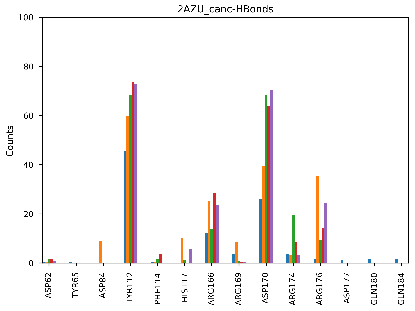
\includegraphics[width=.95\linewidth]{chapter4/2AZU_canc/2AZU_canc-HBonds.pdf}
     \caption{$2AZU_{canc}-HBonds$}
     \label{fig:2AZU_canc-HBonds}
   \end{subfigure}
   \\
   \begin{subfigure}{.45\textwidth}
     \centering
     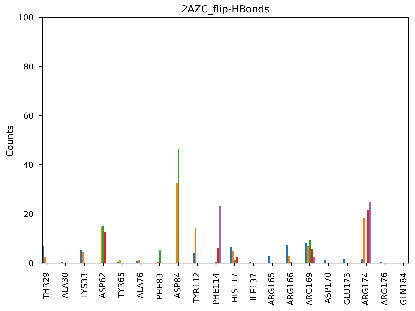
\includegraphics[width=.95\linewidth]{chapter4/2AZC_flip/2AZC_flip-HBonds.pdf}
     \caption{$2AZC_{flip}-HBonds$}
     \label{fig:2AZC_flip-HBonds}
   \end{subfigure}
    \begin{subfigure}{.45\textwidth}
     \centering
     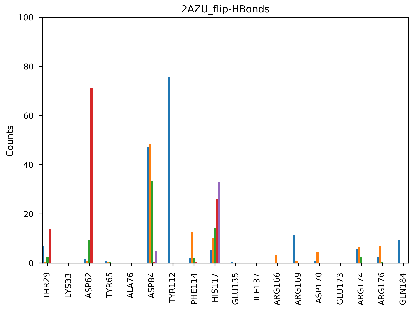
\includegraphics[width=.95\linewidth]{chapter4/2AZU_flip/2AZU_flip-HBonds.pdf}
     \caption{$2AZU_{flip}-HBonds$}
     \label{fig:2AZU_flip-HBonds}
   \end{subfigure}
\caption[H-Bond Contacts for 2AZC/2AZU]{Hydrogen bond contact frequency for 2AZC and 2AZU in the cannonical and flipped binding mode. Each colored bar represents the contact frequency from an individual MD simulation.}
\label{fig:HBonds}
\end{figure}  

In order to gain better insight on the interactions required for catalysis, we profile the hydrogen bond contacts between the ligand and surrounding protein residues.
When comparing the cannonical binding modes, we see that $2AZC_{canc}$ forms hydrogen bond contacts mostly with ASP84, PHE114, HIS117, and ARG176; but no virtually no contact with the catalytic residue ASP62 (Fig. \ref{fig:2AZC_canc-HBonds}).
For $2AZU_{canc}$ (Fig. \ref{fig:2AZU_canc-HBonds}), we see frequent contacts with TYR112, ARG166, ASP170, and ARG176; also, virtually no contact with the catalytic residue ASP62.
Given that we do not see hydrogen bonding between the ligand and ASP62, this supports the hypothesis that the canonical binding mode may not be the pose required for catalysis.

On the other hand, we see a much higher rate of contact to ASP62 with the flipped binding mode, which supports the hypothesis that this binding mode may be what the ligand adopts for catalytic turnover.
In Figure \ref{fig:2AZC_flip-HBonds}, we see ~20\% contact with ASP62 and moderate rates of contact with ASP84, PHE114, HIS117, ARG169, and ARG174.
For $2AZC_{flip}$, contact with ASP62 (yellow/green/red) appears to be related to hydrogen bonding with ASP84 (yellow/green), TYR112(yellow) and ARG174 (yellow).
In Figure \ref{fig:2AZU_flip-HBonds}, we see ~70\% contact with ASP62 and moderate contacts with THR29, ASP84, TYR112, and HIS117.
For $2AZU_{flip}$, contact with ASP62(green/red) appears to be related to hydrogen bonding with THR29(red), ASP84(green) and HIS117(green/red).

\subsection{Comparison to X-ray Crystal Structures}

\begin{figure}[!ht]
\centering
\begin{subfigure}{.5\textwidth}
  \centering
  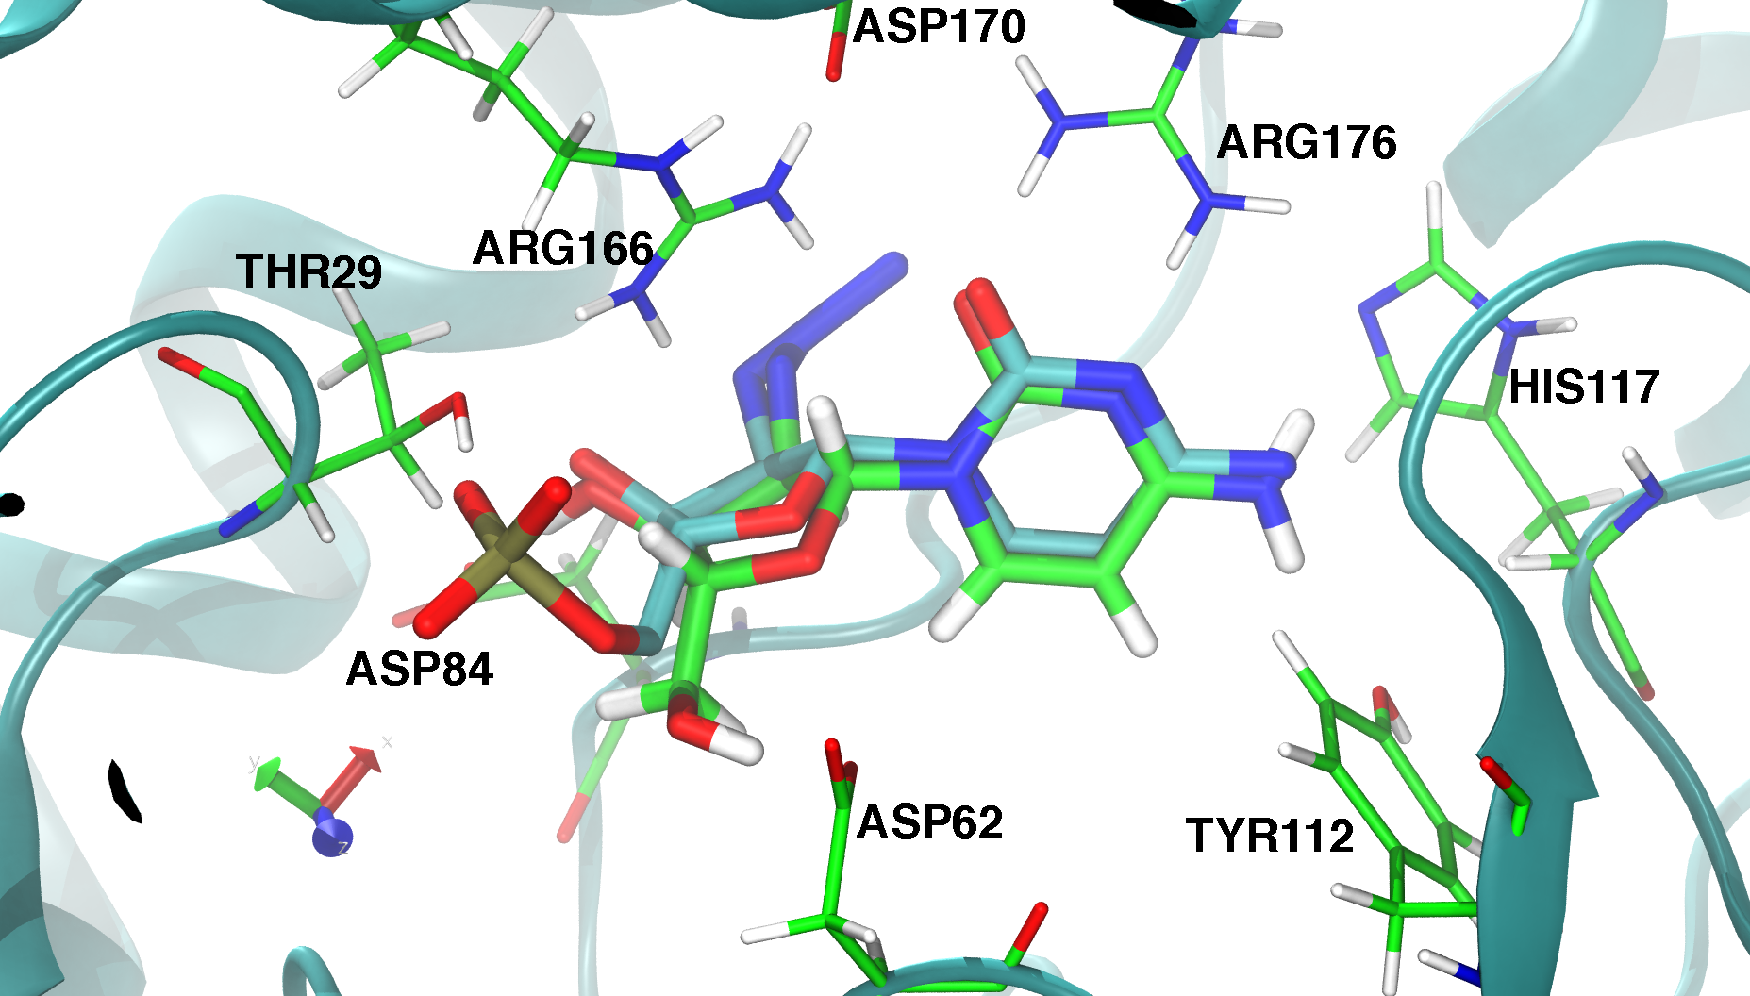
\includegraphics[width=.9\linewidth]{chapter4/xtal/2AZC_canc-xtal_front.pdf}
  \caption{$2AZC_{canc}$}
  \label{fig:2AZC-xtal}
\end{subfigure}%
\begin{subfigure}{.5\textwidth}
  \centering
  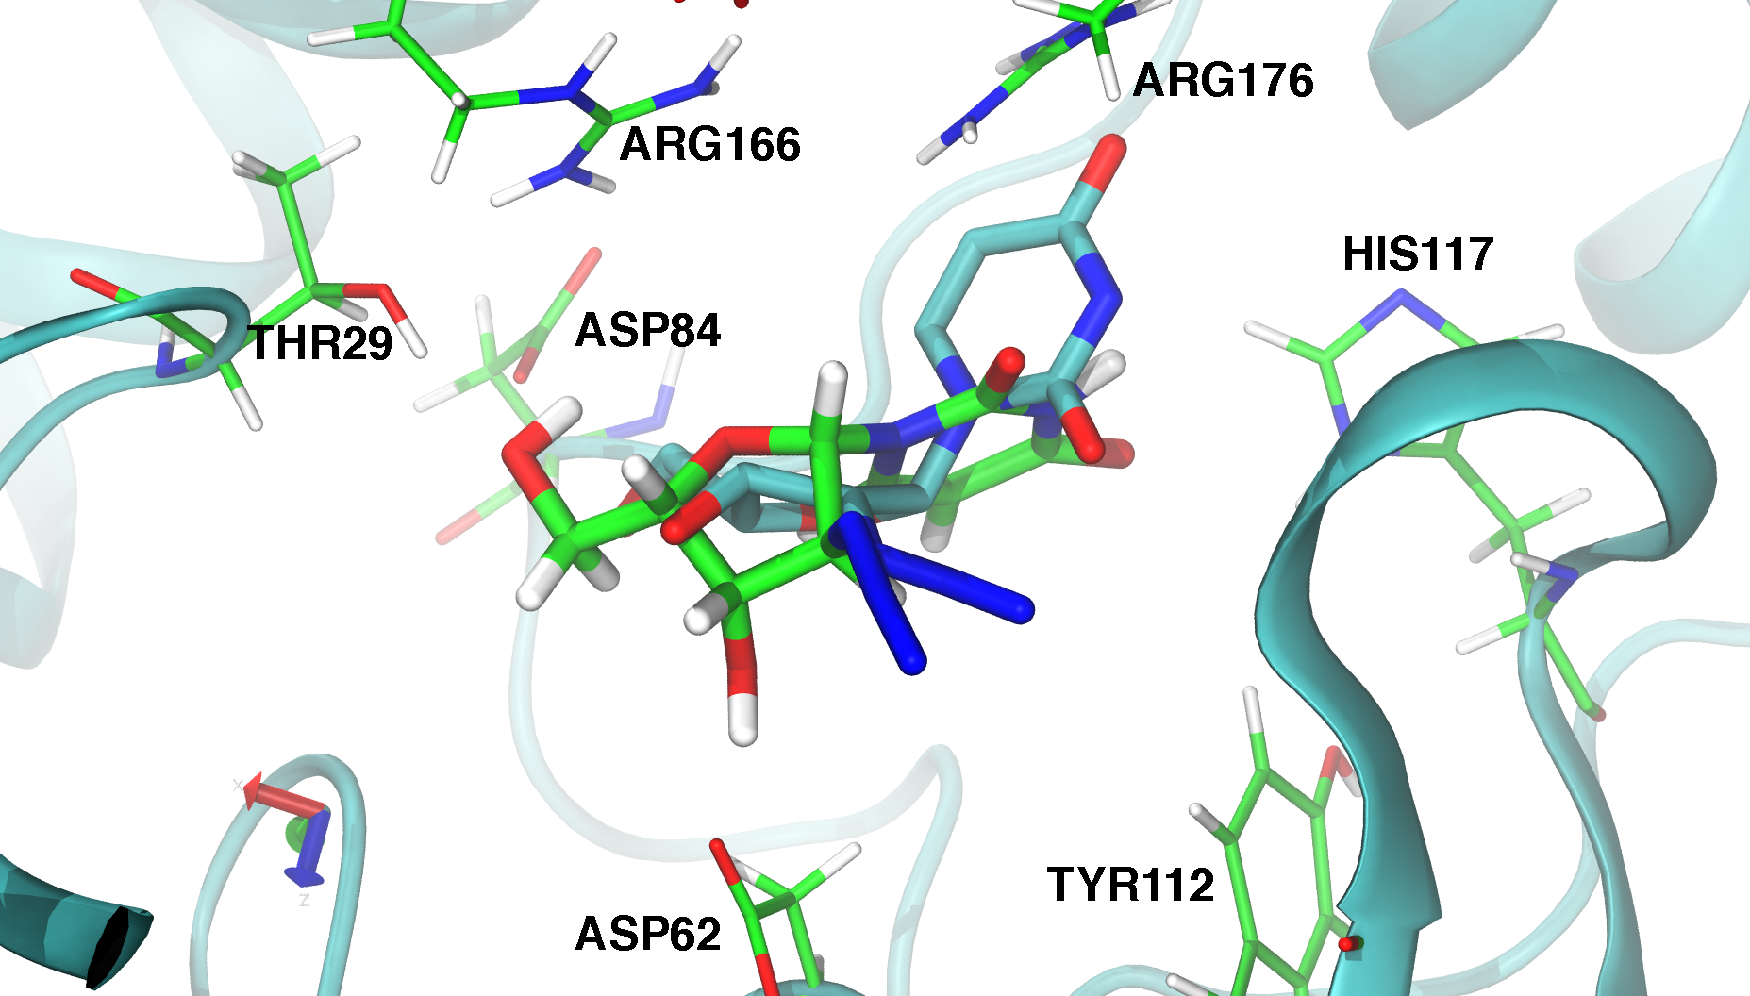
\includegraphics[width=.9\linewidth]{chapter4/xtal/2AZU_flip-xtal_front.pdf}
  \caption{$2AZU_{flip}$}
  \label{fig:2AZU-xtal}
\end{subfigure}
\caption[2AZC/2AZU Comparison to Crystal Structures]{Fig.\ref{fig:2AZC-xtal} shows $2AZC_{canc}$ from MD (green) and the binding mode from crystallography, taken from subunit A (cyan). Fig.\ref{fig:2AZU-xtal} shows $2AZU_{flip}$ from MD (green) and the binding mode from from crystallography, taken from subunit F (cyan). }
\label{fig:xtal}
\end{figure}


\begin{table}[!ht]
\begin{tabular}{|l|l|l|}
\hline
                          & \textbf{$2AZC_{xtal}$} & \textbf{$BB_{RMSD}$} \\ \hline
\textbf{$2AZC_{canc}$} & 0.7                  & 1.2             \\ \hline
\textbf{$2AZC_{flip}$} & 5.0                  & 1.5              \\ \hline
\textbf{}                 & \textbf{$2AZU_{xtal}$} & \textbf{$BB_{RMSD}$} \\ \hline
\textbf{$2AZU_{canc}$} & 4.8                  & 2.7             \\ \hline
\textbf{$2AZU_{flip}$} & 2.3                  & 2.8              \\ \hline
\end{tabular}
\end{table}

Here, we compared our defined metastable binding modes from our MD simulations to our x-ray crystal structures by computing the RMSD between matching heavy atoms in the respective ligands.
The minimum computed RMSD of $2AZC_{canc}$ was 0.7\angstrom and was 5.0 for $2AZC_{flip}$.
Figure \ref{fig:2AZC-xtal} illustrates the crystallized ligand (cyan) directly overlays with the most populated metastable binding mode obtained from our MD simulation (green), except for the additional phosphate group found on the crystallized ligand.
The minimum computed RMSD of $2AZU_{flip}$ from our MD simulation against the x-ray crystal structure was 2.3\angstrom; while for $2AZU_{canc}$ was 4.8\angstrom.
Figure \ref{fig:2AZU-xtal} shows that orientation of the nucleobase moiety from our MD simulation (green) differs from the crystallized ligand (cyan).
Additionally, the ribose moiety sits nearly perpendicular to the nucleobase moiety in the binding mode from MD; while in the crystal structure, the nucleobase and ribose moieties are nearly in the same plane.

\section{Discussion and Conclusion}
Prior to running our MD simulations, we had no experimental evidence which suggests the existence of an alternative binding mode.
We first discovered evidence of a flipped binding mode after our HYBRID docking approach with our short equilibration protocol.
After conducting our MD simulations, we later confirmed the existence of the flipped binding mode by comparing our metastable binding modes against the x-ray crystal structures.

From this study, we believe that the canonical binding mode may not be the binding mode the ligand adopts for catalytic turnover.
Considering the crystallized 2AZC ligand was found to contain an additional phosphate group--indicative of the post-catalytic state--and this coincided with our findings from the MD simulations, we have strong evidence that the canonical binding mode represents the pose after catalysis.
This is illustrated by the extremely low RMSD value (0.7\angstrom) against the crystal structure for $2AZC_{canc}$ and the low rate of contact with the catalytic residues ASP62 for both $2AZC_{canc}$ and $2AZU_{canc}$ (Fig. \ref{fig:2AZC_canc-dist} and Fig. \ref{fig:2AZU_canc-dist}).
Contrary to the literature \cite{tanaka2016molecular}, our simulations suggest that ARG176 plays no role in substrate specificity, where we see roughly equivalent hydrogen bonding frequency for both $2AZU_{canc}$ and $2AZC_{canc}$.
Residue ARG176 seems to only serves a role in stabilizing the ligand in the binding site when in the canonical binding mode.
From Figure \ref{sup:2AZC_flip-dist}, we observe several moments in which the ligand $2AZC_{flip}$ comes into closer contact with ARG176 we see the distance with ASP62 increases and vice versa.

Given that we see a much higher contact frequency with ASP62 for the flipped binding mode over the canonical binding mode, we believe that the ligand must adopt the flipped conformation to stably contact ASP62 for catalytic turnover.
Based on the hydrogen bond contact profiles (Fig. \ref{fig:HBonds}), we believe ASP84 plays a critical role in binding both nuceloside analogs and additional contacts with residues TYR112/HIS117 appear to be necessary for facilitating the interaction with ASP62 (Fig. \ref{fig:2AZC_flip-dist} and Fig. \ref{fig:2AZU_flip-dist}) when in the flipped binding mode.
The binding of $2AZC_{flip}$ appears to specifically require contact with either ARG174/ARG176 residues and potentially forms interactions with TYR112 for additional stability (Fig. \ref{fig:2AZC_flip-HBonds}).
In contrast, binding of 2AZU with TYR112 does not appear to facilitate contact with ASP62 (Fig. \ref{fig:2AZU_flip-HBonds}) but does appear important for stabilizing the canonical binding mode (Fig. \ref{fig:2AZU_canc-HBonds}).
For specificity of binding 2AZU, it appears that hydrogen bonding with HIS117 is required and that contact with THR29 serves for additional stability (Fig. \ref{fig:2AZU_flip-HBonds}).

Overall, these results provide strong supporting evidence that the flipped binding mode represents the conformer of the ligand before catalysis; while the canonical binding mode represents the post-catalytic state.

\section{Acknowledgements}

Christopher Bayly and Gaetano Calabro at OpenEye Scientific Software for development of the MD simulation protocol.

\subsection{Author contributions statement}

S.N. conducted the experiment(s),  B.C crystallized the system, and N.M.L conducted the computational experiments.  All authors reviewed the manuscript. 

\section{Supplemental Information}


    

\subsection{MSM and Clustering}

\begin{figure}[!ht]
\centering
\begin{subfigure}{.5\textwidth}
  \centering
  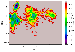
\includegraphics[width=.9\linewidth]{chapter4/2AZC_canc/2AZC_canc-tica.pdf}
  \caption{$2AZC_{canc}-TICA$}
  \label{sup:2AZC_canc-tica}
\end{subfigure}%
\begin{subfigure}{.5\textwidth}
  \centering
  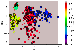
\includegraphics[width=.9\linewidth]{chapter4/2AZC_canc/2AZC_canc-pcca.pdf}
  \caption{$2AZC_{canc}-PCCA$}
  \label{sup:2AZC_canc-pcca}
\end{subfigure}
\caption{PCCA clustering in TICA space from simulations of $2AZC_{canc}$. MD simulations for $2AZC_{canc}$ show sampling of 4 different binding modes (red, yellow, blue, and green), where the dominant binding mode is indicated in red.}
\label{sup:2AZC_canc-cluster}
\end{figure}

\begin{figure}[!ht]
\centering
\begin{subfigure}{.5\textwidth}
  \centering
  \includegraphics[width=.9\linewidth]{chapter4/2AZU_canc/2AZU_canc-tica.pdf}
  \caption{$2AZU_{canc}-TICA$}
  \label{sup:2AZU_canc-tica}
\end{subfigure}%
\begin{subfigure}{.5\textwidth}
  \centering
  \includegraphics[width=.9\linewidth]{chapter4/2AZU_canc/2AZU_canc-pcca.pdf}
  \caption{$2AZU_{canc}-PCCA$}
  \label{sup:2AZU_canc-pcca}
\end{subfigure}
\caption{PCCA clustering in TICA space from simulations of $2AZU_{canc}$. MD simulations for $2AZU_{canc}$ show sampling of 2 different binding modes (pink and red), where the dominant binding mode is shown in pink.}
\label{sup:2AZU_canc-cluster}
\end{figure}

\begin{figure}[!ht]
\centering
\begin{subfigure}{.5\textwidth}
  \centering
  \includegraphics[width=.9\linewidth]{chapter4/2AZC_flip/2AZC_flip-tica.pdf}
  \caption{$2AZC_{flip}-TICA$}
  \label{sup:2AZC_flip-tica}
\end{subfigure}%
\begin{subfigure}{.5\textwidth}
  \centering
  \includegraphics[width=.9\linewidth]{chapter4/2AZC_flip/2AZC_flip-pcca.pdf}
  \caption{$2AZC_{flip}-PCCA$}
  \label{sup:2AZC_flip-pcca}
\end{subfigure}
\caption{PCCA clustering in TICA space from simulations of $2AZC_{flip}$. MD simulations for $2AZC_{flip}$ show sampling of 4 different binding modes (red, pink, blue, and green), where the primary binding mode is indicated in blue.}
\label{sup:2AZC_flip-cluster}
\end{figure}

\begin{figure}[!ht]
\centering
\begin{subfigure}{.5\textwidth}
  \centering
  \includegraphics[width=.9\linewidth]{chapter4/2AZU_flip/2AZU_flip-tica.pdf}
  \caption{$2AZU_{flip}-TICA$}
  \label{sup:2AZU_flip-tica}
\end{subfigure}%
\begin{subfigure}{.5\textwidth}
  \centering
  \includegraphics[width=.9\linewidth]{chapter4/2AZU_flip/2AZU_flip-pcca.pdf}
  \caption{$2AZU_{flip}-PCCA$}
  \label{sup:2AZU_flip-pcca}
\end{subfigure}
\caption{PCCA clustering in TICA space from simulations of $2AZU_{flip}$. MD simulations for $2AZU_{flip}$ show sampling of 3 different binding modes (red, blue and green), where the primary binding mode is indicated in green.}
\label{sup:2AZU_flip-cluster}
\end{figure}
    \subsection{Distance to key residues}

\begin{figure}[!ht]
\centering
  \begin{subfigure}{.45\textwidth}
     \centering
     \includegraphics[width=.95\linewidth]{chapter4/2AZC_canc/2AZC_canc-dist_0.pdf}
  \end{subfigure}
  \begin{subfigure}{.45\textwidth}
     \centering
     \includegraphics[width=.95\linewidth]{chapter4/2AZC_canc/2AZC_canc-dist_1.pdf}
  \end{subfigure}
  \\
  \begin{subfigure}{.45\textwidth}
     \centering
     \includegraphics[width=.95\linewidth]{chapter4/2AZC_canc/2AZC_canc-dist_2.pdf}
  \end{subfigure}
    \begin{subfigure}{.45\textwidth}
     \centering
     \includegraphics[width=.95\linewidth]{chapter4/2AZC_canc/2AZC_canc-dist_4.pdf}
  \end{subfigure}
\caption{Distance to key residues for 2AZC in the canonical binding mode from the other 4 MD simulations, not shown in Fig.\ref{fig:2AZC_canc-dist}. Each colored line represents the contact distance to a key residue.}
\label{sup:2AZC_canc-dist}
\end{figure}  


\begin{figure}[!ht]
\centering
  \begin{subfigure}{.45\textwidth}
     \centering
     \includegraphics[width=.95\linewidth]{chapter4/2AZU_canc/2AZU_canc-dist_0.pdf}
  \end{subfigure}
  \begin{subfigure}{.45\textwidth}
     \centering
     \includegraphics[width=.95\linewidth]{chapter4/2AZU_canc/2AZU_canc-dist_1.pdf}
  \end{subfigure}
  \\
  \begin{subfigure}{.45\textwidth}
     \centering
     \includegraphics[width=.95\linewidth]{chapter4/2AZU_canc/2AZU_canc-dist_2.pdf}
  \end{subfigure}
    \begin{subfigure}{.45\textwidth}
     \centering
     \includegraphics[width=.95\linewidth]{chapter4/2AZU_canc/2AZU_canc-dist_3.pdf}
  \end{subfigure}
\caption{Distance to key residues for 2AZU in the canonical binding mode from the other 4 MD simulations, not shown in Fig.\ref{fig:2AZU_canc-dist}. Each colored line represents the contact distance to a key residue.}
\label{sup:2AZU_canc-dist}
\end{figure}  

\begin{figure}[!ht]
\centering
  \begin{subfigure}{.45\textwidth}
     \centering
     \includegraphics[width=.95\linewidth]{chapter4/2AZC_flip/2AZC_flip-dist_0.pdf}
  \end{subfigure}
  \begin{subfigure}{.45\textwidth}
     \centering
     \includegraphics[width=.95\linewidth]{chapter4/2AZC_flip/2AZC_flip-dist_1.pdf}
  \end{subfigure}
  \\
  \begin{subfigure}{.45\textwidth}
     \centering
     \includegraphics[width=.95\linewidth]{chapter4/2AZC_flip/2AZC_flip-dist_2.pdf}
  \end{subfigure}
    \begin{subfigure}{.45\textwidth}
     \centering
     \includegraphics[width=.95\linewidth]{chapter4/2AZC_flip/2AZC_flip-dist_4.pdf}
  \end{subfigure}
\caption{Distance to key residues for 2AZC in the flipped binding mode from the other 4 MD simulations, not shown in Fig.\ref{fig:2AZC_flip-dist}. Each colored line represents the contact distance to a key residue.}
\label{sup:2AZC_flip-dist}
\end{figure}  

\begin{figure}[!ht]
\centering
  \begin{subfigure}{.45\textwidth}
     \centering
     \includegraphics[width=.95\linewidth]{chapter4/2AZU_flip/2AZU_flip-dist_0.pdf}
  \end{subfigure}
  \begin{subfigure}{.45\textwidth}
     \centering
     \includegraphics[width=.95\linewidth]{chapter4/2AZU_flip/2AZU_flip-dist_1.pdf}
  \end{subfigure}
  \\
  \begin{subfigure}{.45\textwidth}
     \centering
     \includegraphics[width=.95\linewidth]{chapter4/2AZU_flip/2AZU_flip-dist_2.pdf}
  \end{subfigure}
    \begin{subfigure}{.45\textwidth}
     \centering
     \includegraphics[width=.95\linewidth]{chapter4/2AZU_flip/2AZU_flip-dist_3.pdf}
  \end{subfigure}
\caption{Distance to key residues for 2AZU in the flipped binding mode from the other 4 MD simulations, not shown in Fig.\ref{fig:2AZU_flip-dist}. Each colored line represents the contact distance to a key residue.}
\label{sup:2AZU_flip-dist}
\end{figure}  
%%%%%%%%%%%%%%%%%%%%%%%%%%%%%%%%%%%%%%%%%%%%%%%%%%%%%%%%%%%%%%%%%%%%%
%% This is a (brief) model paper using the achemso class
%% The document class accepts keyval options, which should include
%% the target journal and optionally the manuscript type. 
%%%%%%%%%%%%%%%%%%%%%%%%%%%%%%%%%%%%%%%%%%%%%%%%%%%%%%%%%%%%%%%%%%%%%
\documentclass[journal=jcisd8,manuscript=article]{achemso}

%%%%%%%%%%%%%%%%%%%%%%%%%%%%%%%%%%%%%%%%%%%%%%%%%%%%%%%%%%%%%%%%%%%%%
%% Place any additional packages needed here.  Only include packages
%% which are essential, to avoid problems later. Do NOT use any
%% packages which require e-TeX (for example etoolbox): the e-TeX
%% extensions are not currently available on the ACS conversion
%% servers.
%%%%%%%%%%%%%%%%%%%%%%%%%%%%%%%%%%%%%%%%%%%%%%%%%%%%%%%%%%%%%%%%%%%%%
\usepackage{graphicx}
\usepackage[table,xcdraw]{xcolor}
\usepackage{subcaption}
\usepackage{xr-hyper}
\usepackage{hyperref}
\usepackage{microtype}
\PassOptionsToPackage{unicode=true}{hyperref} % options for packages loaded elsewhere
\PassOptionsToPackage{hyphens}{url}
\usepackage{lmodern}
\usepackage{amssymb,amsmath}
\usepackage{ifxetex,ifluatex}
\raggedbottom

\ifnum 0\ifxetex 1\fi\ifluatex 1\fi=0 % if pdftex
  \usepackage[T1]{fontenc}
  \usepackage[utf8]{inputenc}
  \usepackage{textcomp} % provides euro and other symbols
\else % if luatex or xelatex
  \usepackage{unicode-math}
  \defaultfontfeatures{Ligatures=TeX,Scale=MatchLowercase}
\fi
\usepackage{longtable,booktabs}
\usepackage{graphicx,grffile}
\makeatletter
\def\maxwidth{\ifdim\Gin@nat@width>\linewidth\linewidth\else\Gin@nat@width\fi}
\def\maxheight{\ifdim\Gin@nat@height>\textheight\textheight\else\Gin@nat@height\fi}
\makeatother
% Scale images if necessary, so that they will not overflow the page
% margins by default, and it is still possible to overwrite the defaults
% using explicit options in \includegraphics[width, height, ...]{}
\setkeys{Gin}{width=\maxwidth,height=\maxheight,keepaspectratio}
\setlength{\emergencystretch}{3em}  % prevent overfull lines
\providecommand{\tightlist}{%
  \setlength{\itemsep}{0pt}\setlength{\parskip}{0pt}}
\setcounter{secnumdepth}{0}
% Redefines (sub)paragraphs to behave more like sections
\ifx\paragraph\undefined\else
\let\oldparagraph\paragraph
\renewcommand{\paragraph}[1]{\oldparagraph{#1}\mbox{}}
\fi
\ifx\subparagraph\undefined\else
\let\oldsubparagraph\subparagraph
\renewcommand{\subparagraph}[1]{\oldsubparagraph{#1}\mbox{}}
\fi

% set default figure placement to htbp
\makeatletter
\def\fps@figure{htbp}
\makeatother
%%%%%%%%%%%%%%%%%%%%%%%%%%%%%%%%%%%%%%%%%%%%%%%%%%%%%%%%%%%%%%%%%%%%%
%% If issues arise when submitting your manuscript, you may want to
%% un-comment the next line.  This provides information on the
%% version of every file you have used.
%%%%%%%%%%%%%%%%%%%%%%%%%%%%%%%%%%%%%%%%%%%%%%%%%%%%%%%%%%%%%%%%%%%%%
%%\listfiles

%%%%%%%%%%%%%%%%%%%%%%%%%%%%%%%%%%%%%%%%%%%%%%%%%%%%%%%%%%%%%%%%%%%%%
%% Place any additional macros here.  Please use \newcommand* where
%% possible, and avoid layout-changing macros (which are not used
%% when typesetting).
%%%%%%%%%%%%%%%%%%%%%%%%%%%%%%%%%%%%%%%%%%%%%%%%%%%%%%%%%%%%%%%%%%%%%
\newcommand*\mycommand[1]{\texttt{\emph{#1}}}

%%%%%%%%%%%%%%%%%%%%%%%%%%%%%%%%%%%%%%%%%%%%%%%%%%%%%%%%%%%%%%%%%%%%%
%% Meta-data block
%% ---------------
%% Each author should be given as a separate \author command.
%%
%% Corresponding authors should have an e-mail given after the author
%% name as an \email command. Phone and fax numbers can be given
%% using \phone and \fax, respectively; this information is optional.
%%
%% The affiliation of authors is given after the authors; each
%% \affiliation command applies to all preceding authors not already
%% assigned an affiliation.
%%
%% The affiliation takes an option argument for the short name.  This
%% will typically be something like "University of Somewhere".
%%
%% The \altaffiliation macro should be used for new address, etc.
%% On the other hand, \alsoaffiliation is used on a per author basis
%% when authors are associated with multiple institutions.
%%%%%%%%%%%%%%%%%%%%%%%%%%%%%%%%%%%%%%%%%%%%%%%%%%%%%%%%%%%%%%%%%%%%%
\author{Linh P. Nguyen}
\author{Nathan M. Lim}
\author{Gregory Warren}
\author{David L. Mobley}
\affiliation[University of California---Irvine]
{Department of Pharmaceutical Sciences, University of California---Irvine, Irvine, California 92697, United States}
\email{dmobley@mobleylab.org}

%%%%%%%%%%%%%%%%%%%%%%%%%%%%%%%%%%%%%%%%%%%%%%%%%%%%%%%%%%%%%%%%%%%%%
%% The document title should be given as usual. Some journals require
%% a running title from the author: this should be supplied as an
%% optional argument to \title.
%%%%%%%%%%%%%%%%%%%%%%%%%%%%%%%%%%%%%%%%%%%%%%%%%%%%%%%%%%%%%%%%%%%%%
\title{Microsecond molecular dynamics simulations for fragment pose prediction}
%%%%%%%%%%%%%%%%%%%%%%%%%%%%%%%%%%%%%%%%%%%%%%%%%%%%%%%%%%%%%%%%%%%%%
%% Some journals require a list of abbreviations or keywords to be
%% supplied. These should be set up here, and will be printed after
%% the title and author information, if needed.
%%%%%%%%%%%%%%%%%%%%%%%%%%%%%%%%%%%%%%%%%%%%%%%%%%%%%%%%%%%%%%%%%%%%%
\abbreviations{IR,NMR,UV,MD}
\keywords{American Chemical Society, \LaTeX}

%%%%%%%%%%%%%%%%%%%%%%%%%%%%%%%%%%%%%%%%%%%%%%%%%%%%%%%%%%%%%%%%%%%%%
%% The manuscript does not need to include \maketitle, which is
%% executed automatically.
%%%%%%%%%%%%%%%%%%%%%%%%%%%%%%%%%%%%%%%%%%%%%%%%%%%%%%%%%%%%%%%%%%%%%
\begin{document}

%%%%%%%%%%%%%%%%%%%%%%%%%%%%%%%%%%%%%%%%%%%%%%%%%%%%%%%%%%%%%%%%%%%%%
%% The "tocentry" environment can be used to create an entry for the
%% graphical table of contents. It is given here as some journals
%% require that it is printed as part of the abstract page. It will
%% be automatically moved as appropriate.
%%%%%%%%%%%%%%%%%%%%%%%%%%%%%%%%%%%%%%%%%%%%%%%%%%%%%%%%%%%%%%%%%%%%%
\begin{tocentry}
Some journals require a graphical entry for the Table of Contents.
This should be laid out ``print ready'' so that the sizing of the
text is correct.

Inside the \texttt{tocentry} environment, the font used is Helvetica
8\,pt, as required by \emph{Journal of the American Chemical
Society}.

The surrounding frame is 9\,cm by 3.5\,cm, which is the maximum
permitted for  \emph{Journal of the American Chemical Society}
graphical table of content entries. The box will not resize if the
content is too big: instead it will overflow the edge of the box.

This box and the associated title will always be printed on a
separate page at the end of the document.
\end{tocentry}

%%%%%%%%%%%%%%%%%%%%%%%%%%%%%%%%%%%%%%%%%%%%%%%%%%%%%%%%%%%%%%%%%%%%%
%% The abstract environment will automatically gobble the contents
%% if an abstract is not used by the target journal.
%%%%%%%%%%%%%%%%%%%%%%%%%%%%%%%%%%%%%%%%%%%%%%%%%%%%%%%%%%%%%%%%%%%%%
\begin{abstract}
One of the major challenges medicinal chemists face in early drug discovery is the determination of ligand binding modes.
By understanding how a ligand orients itself within a binding site, chemists can gain insight on key interactions for binding and may begin to rationalize how to improve or design a potential lead compound. 
In this retrospective blinded study, we apply routine computational methods such as docking and molecular dynamics (MD) simulations to identify the binding modes on a set of fragment-like molecules bound to soluble epoxide hydrolase (sEH).
Here, we investigate each method's effectiveness in predicting the dominant binding mode and identifying any additional binding modes (if any), then validate our predictions to experimentally obtained X-ray crystal structures.
A set of 19 small molecules were docked into the apo protein crystal structure and then subsequently simulated for 1 microsecond each via MD.
To define ligand binding modes from our MD simulations, we construct Markov state models (MSMs) and analyze our results through a combination of Time-lagged Component Analysis (tICA) with Perron-clustering Cluster Analysis (PCCA).
We are particularly interested in determining whether exchanges between different stable binding modes can happen an adequate number of times at this timescale.
Given that these molecules are small and fragment-like, we expect switching of binding modes to occur relatively more quickly than typical drugs or biomolecules.
In this study, even with simulations at the microsecond timescale for small fragment-like molecules, we do not observe sufficient enough transitions to adequately sample and identify all crystallographic binding modes. 
\end{abstract}

\section{Introduction}
Early stage drug discovery commonly employs high-throughput screening (HTS), where millions of molecules (from small fragments to drug-like compounds) are screened against a target of interest to reveal potential hits.
However, HTS campaigns are expensive and often have low hit rates due to the vastness of chemical space and complexity of therapeutic targets \cite{erlanson_introduction_2012}.
Fragment-based drug discovery (FBDD) campaigns often begin their search through chemical libraries starting with smaller molecules (fragments) to cover a larger fraction of chemical space with the hope of yielding a higher probability of viable hits, even if initially less potent.
Hits obtained from FBDD are often weak binders but serve as a starting point for building lead compounds\cite{erlanson_tethering:_2004}.

Medicinal chemists typically use hits as a starting scaffold or connect fragments together in order to improve binding.
It is at this point in which determining the binding mode may be key for further improvement in the compounds' design \cite{gozalbes_contributions_2010}. 
Knowledge of how a fragment binds suggests key interactions to target for  improving binding and the consequences of scaffold modification.
It is also possible that a fragment may bind in several ways, whereby multiple binding modes contribute to the overall binding affinity \cite{stjernschantz_improved_2010}. 
Thus, in order to improve ligand binding affinity, a medicinal chemist must gain structural insight on the fragments binding mode or binding modes to have some guidance for further design and optimization.

Gaining structural insight to fragment binding modes by experimental methods often poses some challenges. 
Experimental methods for the determination of ligand binding modes include X-ray crystallography, nuclear magnetic resonance (NMR), and surface plasmon resonance.
However, these experimental methods can be costly, time-consuming, and difficult overall\cite{jhoti_fragment-based_2007, gozalbes_contributions_2010}.
Experimental methods such as X-ray crystallography often describe only the single (dominant) binding mode, if one is able to obtain crystals in high enough resolution.
The common problem in FBDD, with x-ray crystallography is that densities obtained in crystal structures can be ambiguous or in too low resolution to definitively resolve the binding mode of their compound.
Inherent to their size, small molecules and fragments often bind in multiple orientations which produce ambiguous densities in the crystal structure \cite{domagalski_quality_2014}.
This is where computational techniques and modelling may aid in the drug development process, by resolving ambiguities in crystal structures and predicted binding modes from computational techniques can help to make sense of partial occupancy data, helping to rescue structure-based design work for fragments.
When computational techniques become accurate enough, it could be employed even when structures aren't available\cite{erlanson_introduction_2012}.

Docking and molecular dynamics provide valuable tools to help determine fragment binding modes \cite{Rocklin2013BlindSite, durrant_computer-aided_2010, sliwoski_computational_2014}. 
Docking is a computationally inexpensive method that takes a static structure of a protein and places a given molecule in a variety of poses, generating a substantial number of candidate binding poses. 
This approach sacrifices accuracy but achieves high speeds by neglecting dynamics in the protein structure.
Although docking can be fast, there is difficulty in determining which of the generated candidate poses represent the relevant or true binding modes.
Dependent on the docking software used, each will score the placement of the ligand using a variety of metrics, usually based on fit within the binding site and scores which might provide rough estimates of protein-ligand interaction energies.
From docking scores, one may guess which molecules to carry forward to subsequent experiments, but docking scores are an unreliable metric for separating molecules that bind from those that do not bind \cite{lape_comparison_2010, plewczynski_can_2011, ramirez_is_2018, gohlke_knowledge-based_2000, warren_critical_2006}.
Docking has shown success in surveying the conformational space of the ligand, but has not proven completely accurate in producing experimentally discovered ligand binding modes \cite{guedes_receptorligand_2013, warren_critical_2006}.

Molecular dynamics (MD) is a computational method that solves Newton's equation of motions in discrete time steps to estimate the dynamics of the system, simulating in full atomistic detail the motions of a protein-ligand system over time \cite{hospital_molecular_2015, hollingsworth_molecular_2018}.
MD simulations allow protein dynamics to be studied in greater temporal and spatial resolution than experimental methods by simulating molecules in time steps compatible with the fastest motion in the system (i.e. bond vibration at 1-2 fs). 
Protein folding and other large conformational changes have timescales ranges from \(10^{-6}s\) (\(\mu\)s) to \(10^{0}\)s or slower \cite{han_protein_2014}. 
Atomistic MD simulations can routinely simulate timescales ranging from \(10^{-15}s\) (fs) to \(10^{-6}s\) (\(\mu\)s). 

Due to computational cost and lack of adequate conformational sampling, MD simulations are limited to shorter timescales than biologically relevant functions because a great amount of time steps are required to visualize these slow-order processes \cite{salmaso_bridging_2018}. 
In the case of FBDD, MD can capture the transition between ligand binding modes to reveal important stabilizing protein-ligand interactions on expected timescales ranging from nanoseconds to milliseconds.
In some cases, ligand binding mode transitions may even require conformational changes in the protein, where these timescales can go beyond milliseconds, however these longer timescales require a significant amount of computational resources  \cite{schlick_biomolecular_1997,macek_backbone_2007}.
This `timescale gap' between computational methods and biologically relevant timescales has been mediated by recent advancements towards increased sampling of the conformational space and Markov State Model (MSM) construction.
Here, we will evaluate whether sufficient sampling can even occur at the microsecond timescale using MD simulations and MSM construction.
Particularly, we are interested in determining if we can sufficiently sample enough binding mode transitions for our fragment set to obtain the correct populations and identify the dominant binding mode and/or additional binding modes.

\subsection{Fragment binding mode predictions to SEH} 
Soluble epoxide hydrolase (SEH) is a protein which is responsible for binding to specific epoxides, converting them to diols, and is found in nearly all tissues (but are highly concentrated in the liver).
The primary function of SEH is in detoxification, catabolism, and regulation of signaling molecules.
SEH catalyzes the breakdown of epoxyeicosatrienoic acids (EETs), acids with cardiovascular effects such as vasodilation and anti-inflammatory actions. 
Inhibition of SEH will slow the degradation of EETs, which can enhance neuroprotection, cardioprotection, and anti-inflammatory effects. 
In vitro studies with murine models have shown SEH inhibition significantly lowers blood pressure, supporting the hypothesized role of SEH in blood pressure regulation. 
The development of SEH inhibitors have therapeutic potential in cardiovascular diseases, inflammatory diseases, and neurological diseases. \cite{morisseau_impact_2013,morisseau_epoxide_2005,kodani_2014_2015}

In this retrospective study, we apply docking and MD techniques on a set of small fragment-like ligands in soluble epoxide hydrolase (SEH) in order to predict fragment binding modes.
We will determine whether docking and MD simulations can successfully identify the binding mode(s).
Binding modes are defined for the remainder of this paper as experimentally or simulation-determined metastable bound states.
Ligand poses are defined as the positions outputted from docking.
Prediction of ligand binding modes using a docking-MD combined approach has seen success in discriminating the experimental binding mode from challenging decoy poses, when compared to docking techniques alone \cite{liu_exploring_2017,clark_prediction_2016} and long MD simulations (e.g. 1 microsecond) have been used to visualize ligand entry and exit into the binding site \cite{decherchi_ligand_2015}.
Thus, we will evaluate whether 1 microsecond MD simulations provide any additional value after docking in uncovering additional ligand binding modes in this system.

The main objective of this study is to assess the performance of computational techniques such as docking and a combined docking and MD approach in identifying the relevant and dominant ligand binding modes (verified with experimental structures).
We aim to provide some insight to determine how effective computational methods can be in identifying the crystallographic binding mode, finding additional binding modes, or resolve ambiguities in experimental structures.

\section{Methods}

\subsection{Preparation}

\begin{figure}
    \centering
    \includegraphics[width=\linewidth]{Figures/backbonermsd.pdf}
    \caption{RMSD of the SEH backbone, relative to the starting positions, after deleting the N terminal domain over the course of an 80ns MD simulation, averaging at 1.8{\AA}}
    \label{fig:backbonermsd}
\end{figure}
Information given to us by our OpenEye scientific collaborators (Christopher Bayly and Gregory Warren) consisted of the apo-protein SEH structure, the binding site in which to dock, the set of ligands to dock (given as SMILES strings), and the protein-ligand crystal structures after refinement by Warren.
All docking and MD simulations of the ligands were conducted without seeing the protein-ligand crystallographic structures.
The provided SEH structure contained missing residues and was not suitable input for MD simulations.
Instead, we used the apo structure of SEH taken from the Protein Data Bank (PDBID: 5AHX) and filled missing residues using PDBFixer \cite{noauthor_pdbfixer_2019}.

The apo SEH structure was uploaded to PDB2PQR \cite{} to strip waters from the system and assign protonation states at pH 8.5, as recommended by our collaborators, with AMBER parameters using PROPKA3.0\cite{jurrus_improvements_2018,sondergaard_improved_2011,noauthor_propka3:_nodate}. 
Parmed (v3.0.1) was used to convert the PQR file back to a PDB file by loading the structure then saving as a PDB \cite{swails_parameter/topology_2019}.
This corrected apo SEH structure was then aligned to the given SEH structure from OpenEye scientific to utilize the same defined binding site for docking.

The full SEH protein features two domains connected by a natural flexible linker, where the SEH binding site given to us was located in the C-terminal domain.
To reduce computational cost, the opposing domain which did not contain the pre-defined binding site was deleted from our simulated protein structure.
Specifically, resides 225 to 546 from the N-terminus of the protein system were deleted and the structural integrity of the protein was evaluated by analyzing the RMSD of the protein backbone.
The RMSD of the protein backbone averaged at 1.8 {\AA} over the course of a 80 ns MD simulation, indicating that deletion of the N-terminal domain did not affect the integrity of the C-terminal domain \ref{fig:backbonermsd}.
A similar trend in RMSD is observed when the N-terminal domain is retained.

\subsection{Docking}

A set of 47 ligands was obtained from collaborators at OpenEye Scientific which we separated into groups based on similarities in complexity. 
Using OpenEye packages to determine various molecular properties, the molecules were divided into 4 groups based on the number of rotatable bonds and their shape volume.
In this study, we examined the group with few rotatable bonds and small molecular volumes, which consists of 19 molecules.
Rotatable bonds for our data set range from 0 to 3 bonds and the volume of each molecule ranges approximately from 133\(\AA ^3\) to 172\(\AA ^3\).
We examined the group of small-fragment like molecules as we expected to observe more binding mode transitions within the microsecond timescale.
The remainder of the molecules will be reserved for subsequent studies.

\begin{figure}
    \centering
    \includegraphics[width=\linewidth]{Figures/seh-binding-site.png}
    \caption{Soluble Epoxide hydrolase binding site divided by the center cleft, defining two sub cavities denoted as left and right. As we rarely observed transitions between the two sub-caivities, we conduct our analysis of binding modes within each sub-cavity, shown here. }
    \label{fig:sEH-ribbon}
\end{figure}

\begin{figure}
    \centering
    \includegraphics{Figures/2d-molecules.png}
    \caption{2D representations of the ligands used in this study. Each molecule is identified by a 3 character code, where alternate protonation states of select ligands are denoted with a 4 character code (i.g. GVG1/2, and 6TZ1/2). These codes are given to us by Warren.}
    \label{fig:2D-molecules}
\end{figure}

The 19 molecules (Fig. \ref{fig:2D-molecules}) were docked into the binding site, as defined by Warren, using the apo protein structure that we prepared for MD simulations.
In Figure \ref{fig:sEH-ribbon}, we divide the SEH binding site into two general regions (left and right) which are separated by two loops which form a cleft in the center \ref{fig:sEH-ribbon}.
At least one study on SEH has suggested that the left region of the binding site serves as a point of entry/exit to the catalytic domain on the right end of the binding side\cite{lotz_unbiased_2018}.

Using Openmoltools (0.8.3)\cite{eastman_openmm_2017} and OpenEye toolkits, each ligand's SMILES string was used to generate a 3D structure and assigned charges through the AM1BCCSym charging scheme via QUACPAC 2017.10.1 \cite{jakalian_fast_2002}. 
Then, we used OpenEye's OMEGA (20180212) to generate up to 1000 conformers for each ligand to be docked and scored\cite{hawkins_conformer_2010}.
The ligands (with their multiple conformers) were docked--into the docking region defined by Warren--using FRED through OEDock version 3.2.0.2. and then scored by the Chemgauss4 scoring function\cite{mcgann_fred_2011}.


From docking, 50 potential poses were generated and subsequently, up to 2-3 unique binding modes were hand-picked by visual inspection and used for the following for MD simulations.
The unique poses were selected to give us a variety of starting configurations for our MD simulations, and selecting docked poses that were in the different sub-cavities of the protein ensured reasonable coverage of all possible binding modes.
With enough simulation time, we expect the fragments to be able to transition between the sub-cavities and eventually find the correct binding mode.

\begin{figure}
    \centering
    \includegraphics{Figures/topscore-rmsd.png}
    \caption{Relationship between the top scoring pose from docking and RMSD to the crystallographic binding mode. Scores from docking do not correlate with the closeness to the crystallographic pose.}
    \label{fig:topscore_correlation}
\end{figure}

The choice to manually select docked poses for increasing the variety of starting MD configurations over selecting poses with the highest docking score is based on the assumption that the docking score is a poor metric for identifying the actual binding mode \cite{warren_critical_2006}.
Figure \ref{fig:topscore_correlation}, illustrates the calculated RMSD of the top scoring poses in this study, does not correlate with closeness to the crystallographic binding mode.
This finding validates our choice to utilize manual selection of the docked poses for starting our MD simulations.

\subsection{Molecular Dynamics}
The system, compromising of only the C-terminal domain, was parameterized using amber99sbildn force field for the protein \cite{}, the TIP3P water model \cite{} for the solvent, and GAFF2 force field for the ligands \cite{lindorff-larsen_improved_2010}.
The following stages were carried out using OpenMM (version 7.1.1) \cite{eastman_openmm_2017,eastman_openmm_2013}.
A maximum of 30,000 minimization steps was applied and the protein-ligand system was equilibrated for 10ps at 1 atm, 300K, and a pH of 8.5 in three stages where the restraint force used to keep the ligand and protein in their starting positions is decreased with each progressing stage. 
The restraint force constant for each progressive stage was $2.0 \frac{kcal}{mol \cdot \mbox{\AA} ^{2}}$, $0.5 \frac{kcal}{mol \cdot \mbox{\AA} ^{2}}$, and $0.1 \frac{kcal}{mol \cdot \mbox{\AA} ^{2}}$, respectively. 
Unrestrained molecular dynamics simulations of the protein-ligand system were then carried out for 1 microsecond for each of the chosen docked poses.

\subsection{Determining Binding Modes by TICA and PCCA}
From our 1 microsecond MD simulations, we rarely observed transitions between the two sub-cavities.
Thus, we divided the analysis of our simulations, separately analyzing cases where the starting pose was in the left sub-cavity and those where the poses were started in the right sub-cavity.
By separating analysis between each respective side of the binding site, we are able to better distinguish between different binding modes sampled during the course of the simulation. 
This allows us to better understand the transitions among these binding modes rather than the timescale to transition between the two sub-regions in the binding site.
For the rare cases in which we observed transitions between the sub-cavities, the simulation data was treated collectively.
Analysis was conducted on the entirety of the 1 microsecond simulation, with trajectory frames stored for analysis every 40ps.

\begin{figure}
    \centering
    \includegraphics{II6/II6_1-full-tiCA.png}
    \caption{TICA analysis of the conformational dynamics of ligand II6 during a 1 microsecond MD simulation yields three possible metastable binding modes as recognized by the (blue, violet, or black) metastable free energy basins.}
    \label{fig:II6_1_tica-kmeans}
\end{figure}

We use PyEMMA (v2.5.2) to analyze the ligand binding modes sampled during our 1 microsecond MD simulations and used the results to construct Markov State Models (MSM)\cite{scherer_pyemma_2015}. 
Here, we chose the distance from the closest heavy ligand atom to key residues as our feature set and apply time-lagged independent component analysis (tICA) \cite{perez-hernandez_identification_2013} to determine the slowest order parameters. 
Previous studies on the SEH system suggested key residue-ligand interactions were among residues ASP110, TYR158, MET194, TYR241, and VAL273 \cite{lotz_unbiased_2018}. 
After applying a tICA transformation on the distances from the closest heavy ligand atom to key residues, we then used the first two TICA components and generate discrete microstates by k-means clustering (Figure \ref{fig:II6_1_tica-kmeans}).

\begin{figure}
    \centering
    \includegraphics{II6/II6_1-full-tiCA-PCCA.png}
    \caption{Ligand II6 TICA coordinates plot with marked discrete microstates colored to indicate different clusters which define our metastable macrostates or stable ligand binding modes. Adjacent macrostates suggest possible transitions between binding modes.}
    \label{fig:II6_1-TICA-PCCA}
\end{figure}

In tICA space, we plot N discrete microstates (representing individual simulation frames), where N is the square root of the total number of simulation frames (i.e. 5000 simulation frames). 
Following this, we build up our macrostates by assigning each discrete microstate to a macrostate using perron-cluster cluster analysis (PCCA) \cite{roblitz_fuzzy_2013,deuflhard_robust_2005} (Figure \ref{fig:II6_1-TICA-PCCA}).
For each macrostate, we store 100 frames to represent our metastable binding modes sampled from MD.


\begin{figure}
    \centering
    \includegraphics{II6/II6_1-full-implied-timescale.png}
    \caption[SEH Implied Timescales]{Relaxation timescales of ligand II6 implied by a Markov model transition matrix estimated at various lag times up to 300ps. Implied timescales should be independent of the lag time and appear to converge at 100ps. With increasing lag time, implied timescales become more constant. The black line with gray area defines the limit of the timescale at which the model can be resolved, where any processes within this area are generally not resolved. With increasing lag time, more process are not resolved. All the processes for II6 are well resolved. Solid lines correspond to the maximum likelihood MSMs. Shaded areas depict confidence intervals containing 95 percent of the samples generated by Bayesian MSM. The confidence intervals remain constant with increasing lag time for II6. Dashed lines correspond to samples means. }
    \label{fig:II6-implied}
\end{figure}

Choosing an appropriate lag time is crucial in properly analyzing the MD trajectories, where a long lag time may gloss over significant ligand movement and a short lag time may unnecessarily be computationally expensive.
The implied timescales provided insight on the timescales to transition into different states.
Plotting the implied timescales against lag time helps select an MSM lag time that will be long enough to indicate Markovian dynamics and short enough to resolve the processes \cite{wehmeyer_introduction_2018}.
A lag time of 300ps was selected as the implied timescale appeared to become independent of lag time (Figure \ref{fig:II6-implied}). 

\begin{figure}
    \centering
    \includegraphics{II6/II6_1-full-spectra.png}
    \caption{Ligand II6 number of clusters against their respective MSM timescales. With increased clusters, the duration of the timescale each cluster represents decreases. Using the elbow method, we select the number of clusters that will best separate the discrete microstates into macrostates. A suitable number of clusters appears to be 3 clusters. }
    \label{fig:II6_1-spectral}
\end{figure}

The number of metastable states was determined from spectral analysis by plotting the number of clusters vs. their respective timescales, then selecting the number of appropriate clusters based on the elbow method (Figure \ref{fig:II6_1-spectral}).

To illustrate the change in binding modes over time, we plot the ligand RMSD from the starting frame and color each time point by the minimizing the RMSD from our 100 frames representing each macrostate or our metastable binding modes.
We then calculate the populations by computing the frequency or the amount of simulation time spent in each defined binding mode.
This effectively shows the occupancy of each binding mode during the 1 microsecond MD simulation and the RMSD of the ligand over time \ref{fig:II6_bmodes} from the initial docked pose.

\subsection{Comparison to the crystallographic pose}
We evaluated docking and MD for their effectiveness in determining ligand binding modes by calculating the RMSD to the crystallographic pose.
Given our (validated) assumption that docking scores does poorly in indicating closeness to the crystallographic binding mode (Fig. \ref{fig:topscore_correlation}), we have no way of knowing which single pose would minimize the RMSD.
The docked poses simulated in MD should not represent docking RMSD because the docked poses were selected based on increasing the variety of starting configurations for MD and are irrelevant to docking abilities in effectively predicting ligand binding modes.
Reporting the RMSD of the best single docked pose would bias the results in favor of docking and not accurately represent the process of using docking to determine ligand binding modes but would show a rare best case scenario of utilizing docking.
Thus, we report the average RMSD from docking to best represent selecting a pose at random from a pool of generated docked poses.
For docking, we computed the average RMSD (with confidence intervals at 95\%) by randomly drawing 50,000 docked poses (without replacement) from our initial 50 generated docked poses.

Similarly, for MD, we report the average RMSD (with confidence intervals at 95\%) by randomly drawing 10,000 frames from our 100 frames we saved as are representatives of each binding mode sampled from MD.
Average MD RMSD values were calculated to best represent the process of selecting a single frame at random from each macrostate, which represent the metastable binding modes sampled during our MD simulations.
Since we do not know which frame sampled during our MD simulation would minimize the RMSD to the crystallographic binding mode, we cannot report the minimum RMSD from our MD simulations.

In cases where the molecule had a single crystallographic binding mode, the most populated cluster was selected as the predicted pose from MD.
In cases where the molecule had two crystallographic binding mode, the top two populated clusters were selected to represent the predicted binding modes from MD.
In cases where the molecules had multiple crystallographic binding modes, we present the average RMSD of each macrostate that minimizes the computed RMSD to the crystallographic binding mode.
Given that we did not know ahead of the study whether any given molecule would exhibit more than two binding modes in crystallography, nor did we observe more than 3 binding mode transitions in our simulations, we believe our procedure for analysis represents a fair assessment for a blind prediction challenge.
Experimental MD ligand pose RMSD values within 2{\AA} of the crystallography binding mode were considered to have sufficiently predicted the binding mode \cite{warren_critical_2006} \cite{plewczynski_can_2011}. 

We remind the reader that we started simulations using poses from each sub-cavity in the SEH binding site and if the crystallographic pose was only found in one sub-cavity, we discarded the simulation data in the opposing sub-cavity--except if we saw transitions between sub-cavities in our simulations.
Given that we rarely observed transitions between sub-cavities in our 1 microsecond MD simulations, in some sense, our predictions put forth represent an `ideal' scenario, where one knows which sub-cavity that the molecule may bind in before running their simulations. 
In subsequent work we hope to explore methods to enhance the transition rate between sub-cavities.

\section{Results}
Given that we do not know ahead of time which docked pose or simulation frame would minimize the RMSD, we remind the reader that we report average RMSDs to replicate the scenario of randomly picking a docked pose or a single simulation frame from MD to compare against the crystal structure (See Methods:Comparison to the crystallographic pose).

\subsection{Single binding mode predictions}
\begin{figure}
    \centering
    \includegraphics{Figures/cluster3_seh_singlebm.png}
    \caption[SEH MD Single Binding Mode Ligands]{RMSD between crystallographic ligand binding mode and predicted binding mode from docking (blue) and MD (green) for cases with a single crystallographic binding mode. Ligand RMSD values are sorted in ascending order according to MD RMSD. We judge success as predicting a binding mode to be less than or equal to 2 {\AA} (black dashed horizontal line). For ligands with single binding modes, MD simulations generally improve RMSD values from docking.}
    \label{fig:rmsd-singlebm}
\end{figure}

\begin{table}[]
\begin{tabular}{|l|l|l|l|l|}
\hline
\textbf{Ligand} & \textbf{Dock} & \textbf{DockErr} & \textbf{MD} & \textbf{MDErr} \\ \hline
\textbf{JF6}    & 14.6          & \textit{0.1}     & 5.4         & \textit{0.1}   \\ \hline
\textbf{4XH}    & 8.8           & \textit{0.1}     & 3.9         & \textit{0.0}   \\ \hline
\textbf{KJU}    & 5.7           & \textit{0.0}     & 3.4         & \textit{0.0}   \\ \hline
\textbf{TGX}    & 8.5           & \textit{0.1}     & 3.0         & \textit{0.0}   \\ \hline
\textbf{6N6}    & 13.8          & \textit{0.0}     & 11.5        & \textit{0.2}   \\ \hline
\textbf{6N4}    & 7.9           & \textit{0.0}     & 7.5         & \textit{0.1}   \\ \hline
\textbf{8NY}    & 6.1           & \textit{0.0}     & 2.4         & \textit{0.0}   \\ \hline
\textbf{ONR}    & 5.3           & \textit{0.0}     & 1.3         & \textit{0.0}   \\ \hline
\textbf{II6}    & 7.8           & \textit{0.1}     & 1.8         & \textit{0.0}   \\ \hline
\textbf{K2T}    & 4.9           & \textit{0.0}     & 3.2         & \textit{0.0}   \\ \hline
\end{tabular}
\caption{Average RMSDs and error {\AA} for molecules with a single binding mode.}
\label{table:singlebm}
\end{table}


Molecules JF6, 4XH, KJU, TGX, 6N6, 6N4,  8NY, ONR, II6, and K2T each had single crystallography binding mode.
Docking had an average RMSD ({\AA}) of 14.63, 8.82, 5.65, 8.52, 13.83, 7.95, 6.06, 5.27, 7.85, and 4.90 for the molecules respectively.
Our reported confidence intervals (at 95\%) for the average RMSDs for each molecule was under 0.05 {\AA}.
The average RMSD ({\AA}) from the most populated binding mode during MD was 5.43, 3.93, 12.09, 2.97, 11.54, 7.46, 2.43, 1.30, 1.79, 3.24, for the molecules respectively.
These values are noted in Table \ref{table:singlebm}.
None of the molecules with single binding modes yielded an average docking RMSD under the 2 {\AA} cutoff.
From MD, 2/10 molecules (ONR and II6) had an average RMSD under the 2 {\AA} cutoff for ligands.
The average docking RMSD for molecules with a single binding mode was $8.3 \pm 1.1 {\AA}$.
The average MD RMSD for molecules with a single binding mode was $4.3 \pm 1.0 {\AA}$.

\subsection{Dual binding mode predictions}
\begin{figure}
    \centering
    \includegraphics{Figures/cluster3_seh_dualbm.png}
    \caption[SEH MD Dual Binding Mode Ligands]{RMSD between crystallographic ligand binding modes and predicted binding modes from docking (blue) and MD (green) for cases with dual crystallographic binding modes. We judge success as predicting a binding mode to be less than or equal to 2 {\AA} (black dashed horizontal line). }
    \label{fig:rmsd-dualbm}
\end{figure}

\begin{table}[]
\begin{tabular}{|l|l|l|l|l|}
\hline
\textbf{Ligand} & \textbf{Dock} & \textbf{DockErr} & \textbf{MD} & \textbf{MDErr} \\ \hline
\textbf{1P8-0}  & 16.6          & \textit{0.0}     & 6.5         & \textit{0.0}   \\ \hline
\textbf{1P8-1}  & 15.4          & \textit{0.0}     & 15.8        & \textit{0.1}   \\ \hline
\textbf{4VY-0}  & 10.1          & \textit{0.0}     & 8.8         & \textit{0.0}   \\ \hline
\textbf{4VY-1}  & 5.7           & \textit{0.0}     & 5.4         & \textit{0.0}   \\ \hline
\textbf{6NX-0}  & 8.4           & \textit{0.0}     & 0.9         & \textit{0.0}   \\ \hline
\textbf{6NX-1}  & 9.1           & \textit{0.0}     & 7.1         & \textit{0.0}   \\ \hline
\end{tabular}
\caption{Average RMSDs and error {\AA} for molecules with two binding modes.}
\label{table:dualbm}
\end{table}


Molecules 6NX, 4VY, and 1P8 each had two crystallographic binding modes.
Average docking RMSD values against the two crystallographic binding modes for each molecule were 16.6 \& 15.4 (6NX), 10.1 & 5.7 (4VY), and 8.4 \& 9.1 (1P8).
The average RMSD from the top two most populated binding modes from MD were 6.6 & 15.8 (6NX), 11.8 \& 4.7 (4VY), 0.9 \& 7.1 (1P8) (Table \ref{table:dualbm}).
None of the 3 cases with dual binding modes yielded an average docking RMSD under 2 {\AA}.
After MD, molecule 6NX yielded an average RMSD value under 2 {\AA} for only one of the two crystallographic binding modes. 

The average docking RMSD for the molecules with dual binding modes was $10.9 \pm 1.8 {\AA}$.
The average MD RMSD for the molecules with dual binding modes was $7.8 \pm 2.0 {\AA}$. 

\subsection{Multi binding mode predictions}

Molecules 6TZ, GVG, YPN, and KUF have 3, 5, 3, and 6 crystallographic binding modes, respectively.
Molecules 6TZ and GVG were simulated twice with different protonation states, denoted as 6TZ1/6TZ2 and GVG1/GVG2. 
Docking and MD did not yield average RMSDs under 2{\AA}, failing to predict any crystallographic pose for molecules with multiple binding modes.
We note that in cases like GVG1, GVG2, and KUF, our simulations did not sample an equal amount of binding modes as found by crystallography; these are denoted with NF in Table \ref{table:multibm}.
The average docking RMSD for the molecules with multiple binding modes was $9.9 \pm 0.5 {\AA}$.
The average MD RMSD for the molecules with multiple binding modes was $7.3 \pm 0.8 {\AA}$. 

\begin{figure}
    \centering
    \includegraphics{Figures/cluster3_seh_multibm.png}
    \caption[SEH MD Multi Binding Mode Ligands]{RMSD between crystallographic ligand binding modes and predicted binding modes from docking (blue) and MD (green) for cases with multiple crystallographic binding modes. We judge success as predicting a binding mode to be less than or equal to 2 {\AA} (black dashed horizontal line).}
    \label{fig:rmsd-multibm}
\end{figure}

\begin{table}[]
\begin{tabular}{|l|l|l|l|l|}
\hline
\textbf{Ligand} & \textbf{Dock} & \textbf{DockErr} & \textbf{MD} & \textbf{MDErr} \\ \hline
\textbf{6TZ1-0} & 16.6          & \textit{0.0}     & 6.5         & \textit{0.0}   \\ \hline
\textbf{6TZ1-1} & 15.4          & \textit{0.0}     & 15.8        & \textit{0.1}   \\ \hline
\textbf{6TZ1-2} & 10.1          & \textit{0.0}     & 8.8         & \textit{0.0}   \\ \hline
\textbf{6TZ2-0} & 5.7           & \textit{0.0}     & 5.4         & \textit{0.0}   \\ \hline
\textbf{6TZ2-1} & 8.4           & \textit{0.0}     & 0.9         & \textit{0.0}   \\ \hline
\textbf{6TZ2-2} & 9.1           & \textit{0.0}     & 7.1         & \textit{0.0}   \\ \hline
\textbf{GVG1-0} & 9.4           & 0.0              & 9.8         & 0.0            \\ \hline
\textbf{GVG1-1} & 6.7           & 0.0              & 5.2         & 0.0            \\ \hline
\textbf{GVG1-2} & 13.4          & 0.0              & 14.0        & 0.0            \\ \hline
\textbf{GVG1-3} & 8.3           & 0.0              & 10.0        & 0.0            \\ \hline
\textbf{GVG1-4} & 6.4           & 0.0              & 5.1         & 0.0            \\ \hline
\textbf{GVG2-0} & 12.0          & 0.0              & 13.9        & 0.0            \\ \hline
\textbf{GVG2-1} & 10.5          & 0.0              & 4.3         & 0.0            \\ \hline
\textbf{GVG2-2} & 11.0          & 0.1              & NF          & NF             \\ \hline
\textbf{GVG2-3} & 7.8           & 0.0              & 5.9         & 0.0            \\ \hline
\textbf{GVG2-4} & 10.2          & 0.0              & 4.2         & 0.0            \\ \hline
\textbf{YPN-0}  & 10.1          & 0.0              & 4.0         & 0.0            \\ \hline
\textbf{YPN-1}  & 10.6          & 0.1              & 4.8         & 0.0            \\ \hline
\textbf{YPN-2}  & 10.6          & 0.1              & NF          & NF             \\ \hline
\textbf{KUF-0}  & 8.0           & 0.0              & 11.7        & 0.1            \\ \hline
\textbf{KUF-1}  & 9.9           & 0.0              & NF          & NF             \\ \hline
\textbf{KUF-2}  & 7.9           & 0.0              & NF          & NF             \\ \hline
\textbf{KUF-3}  & 12.5          & 0.0              & NF          & NF             \\ \hline
\textbf{KUF-4}  & 13.4          & 0.0              & NF          & NF             \\ \hline
\textbf{KUF-5}  & 13.1          & 0.0              & NF          & NF             \\ \hline
\end{tabular}
\caption{Average RMSDs and error {\AA} for molecules with two binding modes. NF indicates that the binding mode was not found.}
\label{table:multibm}
\end{table}

\section{Discussion}
Our MD simulations were initiated from up to three unique docked poses, giving preference to selecting at least one docked pose for each side of the binding pocket. 
The docked poses were selected to increase the variety of starting positions for MD, ideally a docked position in the left and right sub-cavities and a docked position near the center cleft region.
Ligands with less than three poses were often a result of the docking program not placing the ligand near one of the correct region. 
Here, we hypothesized that docked poses and their scores would not adequately identify the crystallographic pose--which we confirmed at the conclusion of this study \ref{fig:topscore_correlation}.
Instead, docking was used as a means for generating starting positions for our MD simulations and hypothesized that the occupancy (i.e. amount of simulation time spent) for each binding mode would be indicative of finding the crystallographic pose.

In the 50 docked poses generated for each molecule, we found that there were indeed a handful of poses which were within 2 {\AA} of the crystallographic pose.
But, given that the docking score did not correlate with closeness to the crystallographic pose, we could not know \emph{a priori} which of the 50 docked poses represented the crystallographic binding mode.
This suggests that docking and scoring is not an effective approach in itself in general and suggests that a better method, perhaps one like MD, may be more successful at identifying dominant binding modes.

Among the bound structures considered in this study, ligands differed in how many crystallographic binding modes were resolved. 
Some had a single binding mode, others two, and some even exhibited larger numbers of binding modes.
If 1 microsecond long MD simulations were long enough to adequately sample enough binding mode transitions, we expect that the populations from MD should be roughly equivalent to the occupancies found via crystallography.
Given that, we expected fragments which exhibit a single binding mode to be easy to identify, fragments with dual binding modes to be moderately challenging, and fragments with multiple binding modes to be the most difficult.
Surprisingly, we found that 1 microsecond of MD did not result in adequate enough sampling for us to get a high success rate in identifying the crystallographic poses. 
It may be possible that an incorrect force field was selected for our system, preventing a simulation of any length from adequately sampling the binding site.
In the following sections, we present and discuss our findings for ligands which exhibited single, two, or more binding modes.

\subsection{Single binding modes: MD simulations can refine poorly docked poses}
For molecules with a single binding mode, we only had a few success cases (ONR and II6). 
Here, we present our observations from II6 to illustrate a successful scenario. 
Molecule II6 represents one case where docking does poorly, but 1 microsecond of MD results in the molecule eventually finding the crystallographic binding mode.

The other molecules in this subset (besides ONR and II6), illustrate that running 1 microsecond MD simulations after docking generally decreases the RMSD to the crystallographic binding mode, but not within the 2 {\AA} cutoff.
We believe that given more simulation time for the other molecules, we would observe similar behaviors to our observations from our II6 simulations.


\begin{figure}
    \centering
    \includegraphics{II6/II6_1-full-bmodes-freq.png}
    \caption[Ligand II6 Binding Mode Populations]{Top: Populations (\% simulation time) of 3 (red, green, blue) binding modes sampled in 1 microsecond of MD for ligand II6. Bottom: RMSD of ligand II6 relative to starting positions over time. Each time point is colored according to the binding mode the ligand is in.}
    \label{fig:II6_bmodes}
\end{figure}

Molecule II6 has one crystallographic pose (PDB:5ALL) which was not found by docking but was identified by MD.
On average, docking generated poses which were 7.9 {\AA} away from the crystallographic pose.

Our MD simulations of II6 began by selection of one docked pose situated on the right side of the SEH binding pocket.
Figure \ref{fig:II6_bmodes}, illustrates that a short amount of time (~150ns) was spent in the initial docked pose (green).
During the time spent in the initial docked pose (green), we observe high fluctuations in the ligand RMSD, indicating that docking has placed the fragment in an unfavorable pose.
After 200ns, we see a transition into a second binding mode (blue) which the fragment resides in for the remainder of the simulation, indicating favorability, representing the dominant binding mode in this simulation.
This (blue) binding mode from MD was 1.8 {\AA} away from the crystallographic pose. 

\begin{figure}
    \centering
    \includegraphics{II6/BR-II6_1-pcca2-CL.png}
    \caption[Ligand II6 with crystal structure]{The dominant binding mode for ligand II6 represented in orange and the crystallographic pose II6 in gray.}
    \label{fig:II6_pcca2}
\end{figure}

Our observations from II6 suggests that docking has a tendency to place the fragments in an unfavorable pose and that after enough simulation time, MD allows the fragment to eventually relax into a new stable configuration.
Generally, we observe the same trend with the other single binding mode fragments.
That is, docking on average does a poor job in placing the fragment in a favorable configuration but relaxation via MD allows the fragment to settle into a new stable configuration.
Once the fragment has stabilized into this new binding mode, the fragment resides there for the remainder of the simulation.
It is often this second binding mode found--following the initial pose from docking--is representative of the dominant binding mode such as in the case of II6 and ONR or somewhat close (within 4A) such as in 8NY, TGX, K2T, KJU, and 4XH (6/10 cases).
It is important to note that, in cases in which we were successful or close, the simulations started within the right sub-cavitity--a more compact region, in which ligand stabilization occurs more quickly (Fig. \ref{fig:sEH-ribbon}).
For these cases, ligand stabilization into the dominant binding mode often occurs between 200-600ns, well within the 1 microsecond timescale of our simulations.  

\begin{figure}
    \centering
    \includegraphics{JF6/JF6_1_c0-full-bmodes-freq.png}
    \caption[Ligand JF6 Binding Mode Populations]{Top: Populations (\% simulation time) of 2 (red and green) binding modes sampled in 1 microsecond of MD for ligand JF6. Bottom: RMSD of ligand JF6 relative to starting positions over time. Each time point is colored according to the binding mode the ligand is in.}
    \label{fig:JF6_bmodes}
\end{figure}

Crystallographic poses for JF6, 6N4, and 6N6 were found to be in the left side of the binding site, where the pocket is much larger and wider.
The larger sub-cavity allows for there to be many more possible metastabile binding modes that the ligand here explores only slowly because of barriers separating them.
Given this, it is unsurprising that we performed poorly in trying to identify the crystallographic pose via MD.
Here, a larger pocket means we must simulate long enough for the fragment to wander away from the initial docked pose and explore enough different metastable binding modes that it can find the dominant binding mode and remain there for a long period of time.
From figure \ref{fig:JF6_bmodes}, we see that JF6 begins in the initial (red) docked pose and then deviates up to 15 {\AA} away into another binding mode (green).
This (green) binding mode was 5.4 {\AA} away from the crystallographic pose, which is likely a result from not allowing enough simulation time for the fragment to find a more favorable binding mode.
On average, the poses generated from docking were 14.6 {\AA} away from the crystallographic pose.
These findings suggest that for larger pockets, one may need to simulate longer than 1 microsecond in order to get enough simulation time to recover from poor initial placements from docking.

\subsection{Dual and Multiple binding modes: Microsecond MD simulations do not capture enough binding mode transitions}
Here, we present our observations on simulations of 6NX, the sole success case in the subset of ligands which have more than one binding mode.
Generally, across this subset of molecules with multiple binding modes, our observations suggest that 1 microsecond of MD simulations do not capture enough binding mode transitions for us to successfully find the correct dominant binding mode.
In our single successful case of identifying 1 binding mode for 6NX, we do not observe any transitions during the course of the simulation, which furthers our claim that 1 microsecond of MD simulations is not sufficient enough of a timescale to get the correct populations for finding the crystallographic binding mode.

Molecule 6NX has two crystallographic poses (PDB:5AKZ), referred to as 6NX-0 and 6NX-1.
The two crystallographic binding poses for 6NX are located by the cleft region of the SEH binding pocket, on the left side of the protein. 
On average, docking generated poses which were 8.4 {\AA} from 6NX-0 and 9.1 {\AA} from 6NX-1. 

\begin{figure}
    \centering
    \includegraphics{6NX/6NX-docked-label.png}
    \caption[Ligand 6NX Docked Poses]{Ligand 6NX in the 3 chosen docked poses 6NX-c0 (right), 6NX-c1 (left), and 6NX-c2 (left) used to start our MD simulations.}
    \label{fig:6NX-docked}
\end{figure}

Our MD simulations of 6NX began by selection of three uniquely docked poses named 6NX-c0, 6NX-c1, and 6NX-c2 situated on the right, left, and left side of the of the SEH binding pocket, respectively \ref{fig:6NX-docked}. 
Populations from MD simulations that are on the same side of the binding site were combined, therefore 6NX-c1 and 6NX-c2 simulations were combined and 6NX-c0 was analyzed separately.
Populations for 6NX-c0 are not included in this analysis because the crystallographic binding modes are not located in the right side of the binding pocket.
The populations of 6NX-c1 and 6NX-c2 are combined to yield red, green, and blue binding modes with populations of 16\% , 34\% , and 50\% , respectively (Fig. \ref{fig:6NX_c2_bmodes} and Fig. \ref{fig:6NX_c1_bmodes}). 

\begin{figure}
    \centering
    \includegraphics{6NX/6NX_1_c2-full-bmodes-freq.png}
    \caption[Ligand 6NX pose 2 Binding Mode Populations]{Top: Populations (\% simulation time) of 1 (blue) binding modes sampled in 1 microsecond of MD for ligand 6NX (pose 2). Bottom: RMSD of ligand 6NX relative to starting positions over time. Each time point is colored according to the binding mode the ligand is in.}
    \label{fig:6NX_c2_bmodes}
\end{figure}
Figure \ref{fig:6NX_c2_bmodes} illustrates that 6NX-c2 in the cleft region of the SEH binding site (left side) spent the entirety of the simulation in the initial docked pose (blue) and does not transition to any additional binding mode.
This is indicative that binding mode transitions for this particular ligand is either very slow or that additional simulation time is required for observing a transition out of this initial binding mode.
By chance, the docked pose 6NX-c2 we selected as a starting point for our MD simulations, was already close to the crystallographic pose by 0.9 {\AA} which likely partialy explains the lack of binding mode transitions in this simulation.


\begin{figure}
    \centering
    \includegraphics{6NX/6NX_1_c1-full-bmodes-freq.png}
    \caption[Ligand 6NX pose 1 Binding Mode Populations]{Top: Populations (\% simulation time) of 2 (red/green) binding modes sampled in 1 microsecond of MD for ligand 6NX (pose 1). Bottom: RMSD of ligand 6NX relative to starting positions over time. Each time point is colored according to the binding mode the ligand is in.}
    \label{fig:6NX_c1_bmodes}
\end{figure}

Figure \ref{fig:6NX_c1_bmodes} shows that 6NX-c1 on the left of the binding pocket begins in the initial docked pose (red) and has high fluctuations in the ligand RMSD during the first ~30ns of the simulation.
The red binding mode remains for approximately ~325ns, then transitions to another binding mode (green), where it remains till the end of the simulation (~675ns).
This secondary binding mode (green) was 7.1 {\AA} away from the secondary crystallographic binding mode.
In this case, we see that from the initial docked pose the ligand drifts ~12{\AA} away over the course of the 1 microsecond MD simulation.
Here, docking had placed the ligand so far away from the crystallographic pose that the simulation was not long enough for the ligand to find the second crystallographic pose (6NX-1).

In the case of 6NX, even with two simulated poses on the same side of the binding site exploring three total different binding modes, 1 microsecond of MD simulations was not sufficient to identify both crystallographic poses.
In one simulation (6NX-c1), we happened to select a docked pose that was very close to one of the crystallographic poses but saw no binding mode transitions during the MD simulation to uncover the secondary binding mode.
In our other simulation (6NX-c2), docking had poorly placed the ligand so far away that we our simulations did not sample either of the crystallographic poses.
In this case, MD captured only one binding mode transition from one simulated pose (6NX-c2), but neither the binding modes sampled were close to the crystallographic poses due to poor initial placement from docking. 

Our observations from 6NX indicate that 1 microsecond of MD does not sufficiently capture enough binding mode transitions, nor does it appear to be a long enough timescale to correct the poor placements from docking.
We observe the same trend with the other fragments, where there is a lack of binding mode transitions, only seeing at most 3 transitions per simulation.
In all (dual and multiple) binding mode cases but one, neither docking or 1 microsecond of MD proved sufficient in identifying the crystallographic binding modes.
Had the microsecond timescale been sufficient to reliably sample at least two binding modes, we would have at least observed a transition in the 6NX-c1 simulation, allowing us to potentially find the secondary binding mode.
Our findings suggest that MD simulations at the microsecond timescale may be able to find at least one crystallographic pose, but identifying secondary or even more binding modes is not likely without much longer simulations. 

\section{Conclusion}
In this study, we used docking and MD on a set of fragment-like molecules binding to soluble epoxide hydrolase to evaluate each method's effectiveness in predicting the crystallographic poses and whether sufficient sampling of relevant fragment binding modes can occur at a 1 microsecond timescale.
Although docking typically produces a few poses close to the crystallographic binding mode, docking on average performs poorly in predicting the crystallographic binding mode.
Our findings show that in the case of fragments with a single binding mode, a relatively small amount of MD  (~250ns) can refine the poses generated from docking and get close to identifying the crystallographic pose. 
In cases where there are multiple binding modes, we anticipated observing multiple binding mode transitions based on the fragment sized ligands and the relatively weak binding such molecules typically exhibit. However we generally do not see more than 3 transitions in our simulations.
MD may find one crystallographic binding mode, however the lack of binding mode transitions restricts MD from revealing multiple crystallographic binding modes despite simulating for a relatively long timescale of 1 microsecond.
Here, the binding site of SEH was relatively large and we divided the entirety of the binding site into two sub-cavities, expecting to observe transitions between them.
However, transitions between the divided sub-cavities of SEH were rarely observed in our simulations of the molecules on a microsecond timescale.
Without more binding mode transitions, we cannot rely on the populations from MD because we do not observe enough binding mode transitions at the microsecond timescale. 

This highlights the necessity of using enhanced sampling techniques in the future, which could help address the fact that microsecond MD simulations did capture multiple binding mode transitions or transition between sub-cavities.
Improved sampling would allow better predictions of ligand binding modes and collection of more accurate populations, which we could use to identify the ligand binding modes that would be found in crystallography.
In this study, we effectively selected docked poses at random to initiate our MD simulations, but for the most part, these docked poses were too far away from the crystallographic pose in that a microsecond MD simulation was not sufficient enough of a timescale to allow for finding the crystallographic pose.

Instead, future studies could investigate using an automated protocol for selecting a more diverse set of docked poses to have a larger variety of poses as starting structures for our MD simulations.
A wider selection of docked poses could improve the chances that refinement by short MD simulations of approximately 250ns would result in finding the crystallographic binding modes. 
Though, this process could generate multiple poses not related to the experimental binding modes.
This improved approach for selecting initial docked poses in combination with enhanced sampling techniques, could result in starting closer to equilibrium during our simulations, where we would observe sufficient enough transitions between the relevant ligand binding modes.
Through proper sampling, we could rely on the populations in our simulations to determine the likely binding modes as found by crystallography.
An alternate approach which can supplement the analysis of populations is to analyze protein-ligand contacts.

In this study, we show that even when simulating small fragment-like molecules in a large spacious binding pocket, sampling reasonable ligand binding mode transitions is challenging, even with relatively long MD simulations.
This illus rates that convergence, solely with MD simulations, is very slow and highlights the necessity of using an enhanced sampling technique to adequately sample and determine ligand binding modes.
We plan to explore these issues in future work.

\section{Contributors}
Christopher Bayly -- OpenEye Scientific, provided MD Floes
Gaetano Calabro -- OpenEye Scientific, provided MD Floes
Greg Warren -- OpenEye Scientific,  curated crystal structures

\section{Potential Journals}
Journal of Chemical Information and Modelling

\bibliography{references}

\end{document}

%%%%%%%%%%%%%%%%%%%%%%%%%%%%%%%%%%%%%%%%%%%%%%%%%%%%%%%%%%%%%%%%%%%%%
%% The "Acknowledgement" section can be given in all manuscript
%% classes.  This should be given within the "acknowledgement"
%% environment, which will make the correct section or running title.
%%%%%%%%%%%%%%%%%%%%%%%%%%%%%%%%%%%%%%%%%%%%%%%%%%%%%%%%%%%%%%%%%%%%%
\begin{acknowledgement}

Please use ``The authors thank \ldots'' rather than ``The
authors would like to thank \ldots''.

DLM appreciates financial support from the National Institutes of Health (1R01GM108889-01 and 1R01GM124270-01A1). Financial support for N.M.L. was provided by the National Science Foundation Graduate Research Fellowship (DGE-1321846)

\end{acknowledgement}


%NML: Add starting simulation poses and the final binding modes and example notebook.
\chapter{Fragment pose prediction using non-equilibrium candidate Monte Carlo and molecular dynamics simulations} \label{SEH-BLUES}

\small{Authors: Nathan M. Lim*, Meghan Osato, Gregory Warren, David L. Mobley}\\

\section{Abstract}
Part of early stage drug discovery involves determining how molecules may bind to the target protein.
Through understanding where and how your molecules bind, chemists can begin to build ideas on how to design improvements to increase binding affinities.
In this retrospective study, we compare how computational approaches like docking, molecular dynamics (MD) simulations, and a non-equilibrium candidate Monte Carlo (NCMC) based method (NCMC+MD) perform in predicting binding modes for a set of 12 fragment-like molecules which bind to soluble epoxide hydrolase.
We evaluate each method's effectiveness in identifying the dominant binding mode and finding any additional binding modes (if any).
Then, we compare our predicted binding modes to experimentally obtained X-ray crystal structures.
We dock each of the 12 small molecules into the apo-protein crystal structure and then run simulations up to 1 microsecond each.
By studying small and fragment-like molecules, we expect to observe switching of binding modes relatively more quickly than with drug-like or larger molecules.
Following this, we build Markov State Models (MSM) to define our stable ligand binding modes.
We investigate if adequate sampling of ligand binding modes and transitions between them can occur at the microsecond timescale using traditional MD or a hybrid NCMC+MD simulation approach.
Our findings suggest that even with small fragment-like molecules, we do not observe sufficient binding mode sampling and fail to identify all the crystallographic binding modes using microsecond MD simulations, but using NCMC+MD we succeed in sampling all binding modes but do not obtain the correct populations.


\section{Introduction}
High-throughput screening (HTS) is commonly used in early stage drug discovery to identify potential binders or hits.
HTS involves taking a large library of molecules and screening them against a target (e.g. protein)
Hit rates in HTS campaigns are often low, simply due to how vast chemical space can be and the complexity of therapeutic targets \cite{erlanson_introduction_2012}.
One common strategy in fragment-based drug discovery (FBDD) projects is to conduct the screen using smaller molecules (fragments) to cover a larger portion in chemical space which may lead to higher hit rates.
Often in this approach hits tend to be weak binders, but they can serve as a starting point for building a potential lead molecule \cite{erlanson_tethering:_2004}.
From the pool of hits, medicinal chemists may find a desirable starting scaffold or they can build up new molecules by connecting fragments together in hopes to improve binding affinity.
While doing this optimization, chemists must gain an understanding of where and how their molecule binds to their target protein, before they can begin to theorize how to make improvements.

Some experimental approaches to gaining structural insight on ligand binding include X-ray crystallography, nuclear magnetic resonance (NMR), and surface plasmon resonance (SPR).
Each of these approaches present its own set of benefits and challenges but most are costly, time-consuming and difficult \cite{jhoti_fragment-based_2007, gozalbes_contributions_2010}.
For example, X-ray crystallography provides structural information with near atomic-resolution, but obtaining high resolution crystal can be extremely challenging.
Especially with FBDD, resolving the binding mode(s) for small molecules and fragments proves challenging as fragments often bind in several different configurations.
This often produces x-ray structures which have ambiguous densities around the bound ligand or are generally in too low resolution to definitively resolve the fragment binding mode(s) \cite{domagalski_quality_2014}.

Here, with these ambiguous densities in the crystal structures, computational approaches may aid in the design process by resolving ambiguities through predicting fragment binding modes.
Computational methods like docking or molecular dynamics (MD) simulations are some common approaches used in helping to determine fragment binding modes \cite{Rocklin2013BlindSite, durrant_computer-aided_2010, sliwoski_computational_2014}.
If these techniques are accurate enough, computational chemists can apply them to make sense of partial occupancy data and help save structure-based design work which are based on fragments.

Docking is a computationally inexpensive technique which generates a variety of configurations or poses by placing the ligand into a static structure of the apo-protein and subsequently scoring each generated candidate.
It can be performed at high-speeds by neglecting any conformational changes in the protein structures--which often results in sacrificing accuracy--making it difficult to distinguish binders from non-binders \cite{lape_comparison_2010, plewczynski_can_2011, ramirez_is_2018, gohlke_knowledge-based_2000, warren_critical_2006}.
Instead, docking can often be used to understand the conformational space of the ligand and provide some initial insight on how a ligand may fit in the binding site.
Several studies have shown that docking does not reliably find experimental binding modes of ligands \cite{guedes_receptorligand_2013, warren_critical_2006}.
Thus, we use docking to generate a variety of configurations which provide coverage of the entire binding site and use these as starting points for our simulations.

Unlike docking, MD simulations resolve---in full atomistic detail---the overall dynamics of the protein-ligand system by solving Newton's equations of motions in discrete timesteps\cite{hospital_molecular_2015, hollingsworth_molecular_2018}.
This can get very computationally expensive if one wants to simulate biological timescales as MD simulations must take timesteps which are constrained by the fastest motion in the system (i.e. bond vibrations at 1-2 femtoseconds).
One may use schemes like hydrogen mass re-partitioning \cite{hmass_repartition} to enable one to take longer timesteps (i.e. 4fs) by slowing down hydrogen bond stretching, but interesting biological motions occur at much larger timescales necessitating large numbers of timesteps and great computational cost.
Interesting biological motions like protein folding or other large conformational changes have timescales ranges from \(10^{-6}s\) (\(\mu\)s) to \(10^{0}\)s or even longer \cite{han_protein_2014}, requiring extremely long compute times if one aims to capture these types of motions.

Fortunately, recent advancements in technology, like the introduction of computing using graphics processing units (GPUs), have made achieving microsecond (or even millisecond) long MD simulations fairly routine.
Despite using longer timesteps and newer technologies, the utility of MD simulations in the drug discovery process has been hindered by MD's inability to adequately sample the conformational space.
Often, MD simulations of a protein-ligand complex will see the ligand remain trapped in the binding mode the simulation had started in and will fail to capture any transition into alternative binding modes.

For FBDD, MD simulations may hold some value given that fragments are small and rigid enough that transitions between binding modes may occur at shorter timescales.
In this case, MD simulations could then resolve potential binding modes and reveal important stabilizing protein-ligand contacts--that is, if such contacts form on reasonable timescales (nanoseconds to milliseconds).
But in some cases, binding mode transitions may require conformational changes in the protein which may take beyond the millisecond timescale before a transition can even occur \cite{schlick_biomolecular_1997,macek_backbone_2007}.
Although these challenges in adequate sampling of the biologically relevant timescales remain an issue to this day, recent advancements in the field have resulted in new ways to address sampling challenges which we apply within this study.
We note that in this study, we are mostly focused on addressing problems of sampling ligand binding modes that occur in the abscence of slow protein conformational degrees of freedom.

One example of an enhanced sampling approach is a hybrid simulation approach which combines non-equilibrium candidate Monte Carlo (NCMC)\cite{ncmc_paper} move proposals with traditional MD simulations.
We previously implemented this NCMC+MD approach in a software package called BLUES: Binding modes of Ligands Using Enhanced Sampling \cite{BLUES_paper}, which aims to accelerate sampling of ligand binding modes by proposing random rotational moves on the ligand and then runs a conventional MD simulation.
BLUES is similar to using traditional Monte Carlo (MC) moves with MD, except that it uses a gradual non-equilibrium based switching protocol while performing perturbations to the ligand instead of an instantaneous perturbation.
In theory, this allows us to perform larger changes to the ligand, while also increasing acceptance of proposed moves over traditional MC.
With the BLUES approach, we hypothesize that we will observe better sampling of ligand binding modes and be able to identify the experimental ligand binding modes over using traditional MD simulations.
Previous work using BLUES has shown success in accelerating sampling of ligand binding modes in the simple model systems of toluene and iodotoluene bound to the T4 lysozyme L99A mutant \cite{BLUES_paper}.
Here, we are interested in applying BLUES to a more complex target with pharmaceutical relevance to evaluate its utility beyond a simple model system.

In this restrospective study, we are interested in using computational methods to identify binding modes for fragments which bind to a protein called soluble epoxide hydrolase (SEH).
SEH has been hypothesized to have therapeutic potential in cardiovascular diseases, inflammatory diseases, and neurological diseases, which has spurred efforts in developing SEH inhibitors.
Specifically, SEH is involved in the breakdown of epoxyeicosatrienoic acids (EETs), acids with cardiovascular effects such as vasodilation and anti-inflammatory actions.
Through slowing the degradation of EETS (via SEH inhibition), it has been hypothesized to induce neuroprotective, cardioprotective, and anti-inflammatory effects.
In vitro studies with murine models found that SEH inhibition significantly lowered blood pressure, bolstering its hypothesized role in blood pressure regulation \cite{morisseau_impact_2013,morisseau_epoxide_2005,kodani_2014_2015}.

Here, we apply docking, MD, and (NCMC+MD) BLUES simulations on a small set of 12 fragments which bind to SEH and evaluate their effectiveness in identifying their binding modes.
For the remainder of this paper, we define binding modes as experimentally or simulation-determined metastable bound states; ligand poses are defined as the configurations generated from docking.
Prediction of ligand binding modes using MD simulations (in comparison to docking alone) has seen some successes in distinguishing experimental binding modes from decoy poses \cite{liu_exploring_2017,clark_prediction_2016}.
Thus, we will investigate if using microsecond MD simulations or our BLUES  (NCMC+MD) enhanced sampling approach provide any value, beyond docking, for identifying the SEH fragment binding modes.
We will compare poses generated from docking and the metastable binding modes sampled from MD and BLUES against experimentally obtained x-ray crystal structures.
Through this study, we aim to provide insight on the value computational methods can provide in identifying the crystallographic binding modes and finding additional binding modes.

\section{Methods}
\subsection{SEH apo-protein preparation}
Prior to beginning this study, our OpenEye Scientific collaborators provided the SEH structure, the location of the binding site where ligands would be docked, and a set of 47 ligands in the form of SMILES strings.
The initial SEH structure from OpenEye Scientific was missing residues.
We found the apo SEH structure in the Protein Data bank (PDBID:5AHX), built in the missing residues with PDBFixer, and used this structure for the remainder of the study \cite{noauthor_pdbfixer_2019}.
The apo SEH structure was altered using the PDB2PQR web server \cite{pdb2pqr}, which uses PROPKA2.0 to assign residue protonation states.
We protonated residues at pH 8.5 to match experimental conditions, using AMBER parameters \cite{jurrus_improvements_2018,sondergaard_improved_2011,noauthor_propka3:_nodate} and we removed crystallographic waters from the system.
The PQR file was then converted back to a PDB file with ParmEd (v3.0.1).
We aligned the corrected apo SEH structure to the SEH structure provided by OpenEye Scientific to ensure the pre-defined docking site was the same.

\begin{figure}
    \centering
    \includegraphics{chapter6/Figures/fullprotein.png}
    \caption[SEH Complete Protein]{The complete SEH protein structure with the C-terminal domain (left) and the N-terminal domain (right). The docking site is highlighted (blue) in a mesh representation. The N-terminal domain (right) was removed to reduce computational costs, keeping the C-terminal domain with the defined docking site.}
    \label{fig:full-protein}
\end{figure}

\begin{figure}
    \centering
    \includegraphics{chapter6/Figures/protein-bb-rmsd.png}
    \caption[SEH Backbone RMSD after N-terminal domain removal]{Calculated RMSD {\AA} of the protein backbone relative to the starting position for 1 microsecond of MD with an average RMSD of 2.1 {\AA} after removal of the N-terminal domain. The protein backbone eventually stabilizes at 3 {\AA} from the starting position. This indicates that removal of the N-terminal domain did not largely affect the protein structure.}
    \label{fig:protein-bb-rmsd}
\end{figure}

The SEH protein contains 2 domains, a phosphatase domain (N-terminus) and a hydrolase domain (C-terminus) connected by a flexible proline rich linker \cite{doi:10.1021/bi050842g}.
The pre-defined docking site was only located in the C-terminal hydrolase domain, so to reduce computational cost, we removed the N-terminal domain from residue 0 to residue 224 (Fig. \ref{fig:full-protein}).
We analyzed the structural integrity of the truncated protein by averaging the RMSD of the protein backbone over a 1 microsecond MD simulation.
The average RMSD of the truncated protein backbone was 2.1 Angstroms suggesting the C-terminus was relatively unaffected by the removal of N-terminus.
In Figure \ref{fig:truncated-protein}, we show the entire binding site located in the C-terminus domain as defined by our collaborators.

\begin{figure}
    \centering
    \includegraphics{chapter6/Figures/protein-mark.png}
    \caption[Truncated SEH Protein Structure]{Truncated SEH protein structure (C-domain only) with the the docking site is highlighted (blue) in a mesh representation. We divide the full cavity into two sub-cavities denoted by left and right. The sub-cavity division is best denoted at the two loops marked as A and B in the figure. In the SEH apo protein structure, point A is closest to residue VAL381 and point B is closest to residue VAL499. We treat each sub-cavity separately in our analysis to better resolve binding modes within each sub-cavity.}
    \label{fig:truncated-protein}
\end{figure}

Here, we define two sub-cavities (left/right) which are separated by two loops which form at residues VAL381 (A) and VAL499 (B), creating a cleft in the center of the SEH binding site (Fig. \ref{fig:truncated-protein}).
Throughout this study, we treat the left and right sub-cavity separately as we did not observe transitions between them in our simulations.
By performing our analysis on each sub-cavity separately, we are better able to resolve the binding modes and timescales for transitions between binding modes, over trying to resolve the transition timescales between the sub-cavities.

\subsection{Ligand preparation and docking}
\begin{figure}
    \centering
    \includegraphics{chapter6/Figures/2dmolecules.png}
    \caption{}
    \label{fig:2dmolecules}
\end{figure}
From a set of 47 ligands given to us by our OpenEye Scientific collaborators, we chose to study a smaller subset of 12 ligands (Fig. \ref{fig:2dmolecules}).
Here, we chose ligands based on the overall size and number of rotatable bonds.
Particularly, we were interested in only studying small and rigid fragment molecules as we expected to observe more binding mode transitions during our simulations, due to their size and rigidity.
The molecule set ranged from 133.13 to 156.73 ${\AA^{3}}$ in shape volume with 0 to 1 rotatable bonds.

We used openmoltools (v0.8.1) \cite{} and OpenEye toolkits \cite{openeye_toolkit} to convert each ligand SMILES string to a 3D structure and then we assigned charges using the OEAM1BCC \cite{jakalian_fast_2002}. charging scheme from the OEQUAPAC library \cite{jakalian_fast_2002}. .
Then, we generated 1000 conformers of each charged ligand using OpenEye’s OMEGA (20180212) \cite{hawkins_conformer_2010}.
These conformers were then docked into the SEH apo protein structure using FRED from OEDock(v3.2.0.2), generating 1000 docked poses, and scored with the Chemgauss4 scoring function \cite{mcgann_fred_2011}.

\begin{figure}
    \centering
    \includegraphics{chapter6/Figures/topscore.png}
    \caption{Docking score and the calcualted RMSD {\AA} to the crystallographic binding modes from the top scoring docked poses.}
    \label{fig:topscore}
\end{figure}

From the 1000 generated docked poses, we wanted to select the most distinct and use them as our starting positions for our simulations.
Here, we define distinct docked poses as poses which are dissimilar from one another.
Some studies have shown that docking is an unreliable method for identifying the true binding mode using the top scoring pose \cite{warren_critical_2006}.
Given this, we believed that the top scoring poses would often be far from the true binding mode and thus, we did not retain them and use them as starting points for our MD simulations.
Later, we confirmed that the top scoring docked poses are not generally close to the crystallographic binding modes (Fig. \ref{fig:topscore}).

By selecting the distinct poses generated from docking, we have a variety of starting configurations in our simulations and provide reasonable coverage of the protein binding site.
Regardless of the starting positions, given enough simulation time and the fragment-like properties (i.e. small and rigid properties) of the molecules we are simulating, we should see convergence to the true binding mode given the forcefields, protonation states, accuracy of our model, and simulation timescales used in this study.
We describe the filtering and selection process below.

\subsubsection{MDS-RMSD Filtering: Unique pose selection}

\begin{figure}
    \centering
    \includegraphics{chapter6/Figures/GVG_1-rmsd_matrix.png}
    \caption[RMSD Similarity Matrix]{RMSD {\AA} similarity matrix from 1000 docked poses for GVG1. Poses which are similar will have a low RMSD represented by darker colors (blue to purple) and poses which are dissimilar will have a high RMSD represented by brighter colors (green to yellow). This shows the raw similarities between docked poses.}
    \label{fig:similarity_matrix}
\end{figure}

First, we generate a RMSD-based similarity matrix of the 1000 generated docked poses.
That is, we compute the RMSD, using only the ligand heavy atoms, from each docked pose to every other docked pose.
This gives us an $N x N$ similarity matrix (N=1000), in which our measure of similarity is based on the calculated RMSD between the docked poses (Fig. \ref{fig:similarity_matrix}).
Next, we apply a technique called Multi-Dimensional Scaling (MDS) through scikit-learn (v0.19.0) \cite{scikit_mds} in order to reduce our $N x N$ dimensional space into a 2D space, where we can then apply clustering techniques.
MDS is a method which transforms our similarity matrix and projects each object (i.e pose) into a lower dimensional space in such a way that the distance between objects (i.e poses) are preserved as best as possible.
In other words, when we project into a 2D space, poses which are similar (low RMSD) will appear closer together and poses which are dissimilar (high RMSD) will appear farther away.

\begin{figure}
    \centering
    \includegraphics{chapter6/Figures/GVG_1-mds_6.png}
    \caption[Silhouette scoring in MDS-RMSD space]{Left: Silhouette scores from 1000 docked poses for GVG1 using 6 clusters from K-means clustering. Right:MDS-RMSD scatter plot for 1000 docked poses for GVG1 with K-means clustered points using 6 clusters. The cluster centroids are denoted by a number in white circles.}
    \label{fig:mds}
\end{figure}

After applying MDS to our RMSD similarity matrix, we transform our $N x N$ dimensional space and take our first two MDS components to project the data into a 2D scatter plot.
This enables us to easily apply K-means clustering \cite{scikit_kmeans} (from scikit-learn) to group up similar poses and separate dissimilar poses with the first two components which best represent the pair-wise similarity distances.
A notable downside to K-means clustering is that one has to specify the number of clusters to be used to separate the data points.
To avoid bias, we use silhouette scoring \cite{scikit_silhouette} (from scikit-learn) to automatically determine the best number of clusters to use to separate our data points.
Silhouette scoring is a method which ranges from -1 to +1 and evaluates how similar objects belonging to the same cluster are (cohesion) and how dissimilar those objects are with other clusters (separation) (Left: Fig. \ref{fig:mds}).
High values (closer to +1) indicate that the object is similar to other objects within the same cluster and dissimilar to objects in neighboring clusters.
Low values (closer to -1) indicate that the object is dissimilar to others within the same clusters and similar to objects in neighboring clusters.
A low total silhouette score indicates that the clustering configuration is likely incorrect with either too many or too few clusters, so we can use the total silhouette score as a way to select the optimal number of clusters.

We apply K-means clustering using a range of 2-9 (K) clusters on our MDS-RMSD scatter plot and score each round of clustering using silhouette scores.
We selected the number of clusters K maximizing total silhouette score, and then used this to partition our 1000 docked poses in MDS-RMSD space and set the number of starting poses to be used for our simulations.
Using the K clusters which maximized the silhouette score, we then selected the centroid of each cluster as the representative pose for starting our simulations (Right: Fig. \ref{fig:mds}).

\subsection{Molecular Dynamics and BLUES Simulations}
In this study, we used two simulation approaches: traditional molecular dynamics (MD) simulations and our hybrid approach called BLUES: Binding modes of Ligands Using Enhanced Sampling \cite{BLUES_paper}, which combines Non-equilibrium Candidate Monte Carlo (NCMC) \cite{ncmc_paper} move proposals with MD.
Both MD and BLUES simulations using OpenMM (v7.1.1) \cite{openmm} with the same solvated SEH system.
For our simulations, the truncated SEH protein (consisting of only the C-terminal domain) was paramterized with amber99sbildn forcefield for the protein and GAFF2 for the ligands, and solvated with TIP3P waters \cite{lindorff-larsen_improved_2010}.

We performed a maximum of 30,000 energy minimization steps and a 3 stage (NVT, NPT, NPT) equilibration protocol which we describe as follows.
In each equilibration stage, a restraint force is placed on the $\alpha$-Carbons of the protein backbone and the ligand heavy atoms, where we successively decrease the force from $2.0 \frac{kcal}{mol \cdot \mbox{\AA} ^{2}}$ to $0.5 \frac{kcal}{mol \cdot \mbox{\AA} ^{2}}$ to $0.1 \frac{kcal}{mol \cdot \mbox{\AA} ^{2}}$ at each stage.
After equilibration, we ran 1 microsecond ($\mu$s) using molecular dynamics (MD) and 600 nanoseconds (ns) using BLUES for each pose selected by our MDS-RMSD filtering protocol (described in the previous section).
Our simulations were run using 4 femtosecond (fs) timesteps and with the hydrogen-mass repartioning scheme \cite{hmass_repartition}.

Briefly, we describe our protocol for BLUES simulations.
A BLUES simulation begins with the NCMC phase, which involves proposing a random rotation about the ligand center of mass and then relaxes via a series of non-equilibrium switching steps which alchemically scale the ligand interations off/on over $N$ steps.
This is in contrast to traditional Monte Carlo, which involves performing an instantaneous change to the ligand coordinates.
Specifically, interactions are controlled via a parameter ($\lambda_{0 \rightarrow 1}$) which scales the ligand interactions with the surrounding environment.
Our non-equilibrium switching protocol begins with the fully interacting ligand at $\lambda_{0}$ and then we alchemically scale the ligand forces off until $\lambda_{0.5}$, where the ligand is no longer interacting with surrounding atoms.
We perform the proposed random rotation on the non-interacting ligand and then alchemically scale the ligand forces back on until $\lambda_{1}$, where the ligand is fully interacting and in the proposed positions.
Over the series of $N$ NCMC switching steps, we accumulate the total non-equilibrium work done and use this in acceptance or rejection of the proposed move (following the Metropolis-Hasting acceptance criterion \cite{met_hastings_acceptance}).
After the Metropolization step, we follow-up using traditional MD methodology and repeat the cycle (NCMC -> MD -> NCMC...etc.) for $I$ iterations.

\subsection {Determination of Binding Modes with TICA and PCCA}
We divide the SEH binding site (Figure \label{fig:truncated-protein}) into two sub-cavities denoted as ``left'' and ``right'' and analyze simulation data from these two sub-cavities separately, as we rarely observed transitions between them.
That is, simulations which started with dock poses in the right sub-cavity were pooled together and vice versa, but simulations in each sub-cavity were kept separate, since very few simulations exhibited transitions and thus pooling data across sub-cavities would have complicated analysis.
By treating the two sub-cavities separately, we are better able to distinguish between binding modes sampled within each sub-cavity and understand their timescales, over the timescale to transition between sub-cavities.
In other words, we can better distinguish rapid transitions between binding modes within each sub-cavity over the slow transitions between sub-caivities.
Additionally, if we had pooled together simulation data from both sub-cavities, our silhouette scores would always suggest 2 binding modes, which is actually just the separation of binding modes between the two cavities.

\begin{figure}
    \centering
    \includegraphics{chapter6/Figures/GVG_1-right_imptimescales.png}
    \caption[Implied Timescales for GVG1]{Implied timescales plot for GVG1 from our BLUES simulatinos. This plots a series of lag times (picoseconds) versus timescales of various states. The choice of lagtime to discretize our simulation frames was chosen by selecting a lagtime where it begins to become independent of timescales. We chose a lagtime of 400ps.}
    \label{fig:GVG_1-right-imptimescales}
\end{figure}

Using PyEMMA (v2.5.5), we analyzed and built Markov State Models (MSM) separately between our MD and BLUES simulations.
MD simulation frames were stored every 25,000 steps (100ps/frame) and BLUES simulation frames were stored every 10,000 steps (40ps/frame).
In this study, we apply a method called time-lagged indepdent component analysis (TICA) with perron-cluster cluster analysis (PCCA) to define our metastable binding modes sampled during our simulation.
The appropriate lagtime for TICA was chosen by plotting the implied timescales versus a series of lagtimes and selecting a lagtime where the timescales appeared to be independent of lag time (Figure \ref{fig:GVG_1-right-imptimescales}).
Here, $N$ is defined as the square root of the total number of simulation frames, which is the default choice for PyEMMA.
We used lagtimes of 250ps for MD and 400ps for BLUES simulations.

\begin{figure}
    \centering
    \includegraphics{chapter6/Figures/GVG_1-right_c4-tica.png}
    \caption[TICA plots for GVG1]{Time-lagged indepdent component analysis (TICA) plot for binding modes of GVG1 located in the right sub-cavity using the first two TICA components. Discrete microstates (i.e. simulation frames are denoted by black Xs. Metastable states sampled during the simulation are indicated in darker colors (blue-purple) in the contours or where Xs are more dense.}
    \label{fig:GVG_1-right-tica}
\end{figure}

\begin{figure}
    \centering
    \includegraphics{chapter6/Figures/GVG_1-right-pcca.png}
    \caption[PCCA plot for GVG1]{TICA plot for binding modes of GVG1 located in the right sub-cavity using the first two TICA components. Each X denotes a discrete microstate (i.e. simulation frame). Each microstate has been assigned to a macrostate by PCCA which define our metastable binding modes sampled during our simulation. We find 3 states (red, green ,blue) or binding modes sampled from simulations of GVG1 in the right sub-cavity.}
    \label{fig:GVG_1-right-pcca}
\end{figure}

In this study, we analyzed the distances between the ligand heavy atoms and each of residues ASP110, TYR158, MET194, TYR241 and VAL273.
These were chosen because they were highlighted in an experimental study as being key residues for binding (\cite{lotz_unbiased_2018}).
With these distances to key residues as our feature set, we applied TICA \cite{perez-hernandez_identification_2013} to extract the slow order parameters and mapped our simulation frames via k-means clustering.
This gives us a set of $N$ discrete microstates (i.e. simulation frames) into the coordinate space of the first 2 TICA components (Fig. \ref{fig:GVG_1-right-tica}).

In Figure \ref{fig:GVG_1-right-pcca},  we define our macrostates or metastable binding modes, by assigning each microstate to a given $K$ number of macrostates via PCCA \cite{roblitz_fuzzy_2013,deuflhard_robust_2005}.
To determine the appropriate number of $K$ macrostates to use, we evaluate the clustering using silhouette scoring \cite{scikit_kmeans} (discussed previously).
In our analysis we represent each macrostate by randomly draw 100 simulation frames from the pool of microstates assigned to each $K$ macrostates.

In Fig \ref{fig:GVG1_c4-md}, we plot the RMSD of the ligand heavy atoms relative to the starting configuration and color each time point by assigning it to the macrostate which minimizes the RMSD.
Specifically, we compute the ligand heavy atom RMSD to the 100 representative microstates (simulation frames) belonging to each macrostate; then, assign it to the macrostate which minimizes the RMSD.
We can then compute the populations or amount of simulation time spent within each binding mode by counting the membership assignment of the simulation frames.

\subsection {Crystallographic Binding Mode Predictions}
To evaluate the ability to predict dominant binding modes as determined by crystallography using docking, MD, or BLUES, we report two RMSD ({\AA}) metrics: an `averaged' RMSD and the minimum RMSD.
Here, our reported average RMSD is calculated by averaging over 10,000 randomly drawn (with replacement) values from the remaining (MDS-RMSD filtered) docked poses or 100 simulation frames which we saved to represent each binding mode.
We believe this `average' RMSD best represents random selection of a single docked pose from a pool of poses or a single frame from the whole simulation to compare against the crystallographic structure.
We also report the minimum RMSD as this represents the best case or `ideal' scenario where we could identify which structure generated from docking or sample from our simulations would be closest to the crystallographic binding mode. H
owever, we are not aware of any method which could identify such poses so we view minimum RMSD to be useless as a performance metric.
Here, we include it simply to provide a way to assess whether any poses were sampled that were close to the crystallographic bining mode.

We remind the reader that our analysis treats each sub-cavity \ref{fig:truncated-protein},  separately.
There were a total of 29 crystallographic binding modes to be identified out of the 12 ligand we simulated, where molecules fell into 2 groups: those with a single binding mode and those with multiple binding modes (2+).
For ligands with a single binding mode, we report the average and minimum RMSDs (described previously) of the ligand atoms in the crystallographic structure against those in the representative frames from the binding mode with the highest occupancy (i.e simulation time).
When ligands have multiple crystallographic binding modes, we report the lowest RMSD from the binding modes found from simulations, relative to each crystallographic binding mode.
We describe a successful prediction as being within 2 {\AA} of the crystallographic binding mode and close predictions as predictions within 4 {\AA} of the crystallographic binding mode.

\section{Results}
Here, we analyze the success of docking, standard MD and BLUES at recovering crystallographic binding modes of a series of 12 ligands which have a total o 29 binding modes between them.
In our analysis, we consider data only from docked poses or binding modes sampled during our simulations which are in the correct sub-cavity.
That is, if the crystallographic structure was found in the right sub-cavity, we computed the RMSD using docked poses or simulation frames that were only in the right sub-cavity (and vice versa).
In this study, we consider predictions successful when they are within 2 {\AA} of the crystallographic binding mode and we label predictions ``close'' when they are within 4 {\AA}.
There were a total of 29 binding modes to be predicted from our set of 12 molecules simulated.

We remind the reader that we report an `averaged' RMSD from each method (See Methods:Comparison to the crystallographic pose).
Since we cannot determine which docked pose or single simulation frame would result in minimizing the RMSD to the crystallographic binding mode without bias, an averaged RMSD represents randomly picking from a pool of docked poses or a single simulation frame representative of a metastable binding mode.
Note, the reported RMSD from docking is representative of the remaining docked poses after applying our RMSD-MDS filter to the initial pool of 1000 generated docked poses.
Here, we will also report the minimum RMSD to show the best case or `ideal' scenario for each method.
The minimum RMSD reflects the performance which would be expected if one could determine somehow, without knowing the crystal structure, which docked pose or simulation frame would be closest to the true binding mode.

\begin{figure}
    \centering
    \includegraphics{chapter6/Figures/averages.png}
    \caption[Average RMSD]{Minimum/Average RMSD for each method: docking (pink/red), MD (lime/green), and BLUES (cyan/blue) for all ligands in this study. Dashed line at 2 {\AA} represents successful predictions and dotted line at 4 {\AA} represents close predictions. This reports the averaged RMSD from all 12 ligands used in this study.}
    \label{fig:averages}
\end{figure}
Here, we find that no method always correctly identifies the crystallographic binding mode (as evidenced by average RMSD) but both MD and BLUES substantially outperform docking at sampling binding modes near the crystallographic one, and of these, BLUES performs better.
Averaged across all of the ligands in this study,  the minimum RMSDs for docking (pink), MD (lime), and BLUES (cyan) were $3.9 \pm 0.2 {\AA}$, $2.7 \pm 0.3 {\AA}$, and $1.9 \pm 0.2 {\AA}$ respectively; the average RMSD for docking (red), MD (green), and BLUES were $5.9 \pm 0.2 {\AA}$, $5.1 \pm 0.4 {\AA}$, and $4.8 \pm 0.3 {\AA}$ respectively ( (Fig. \ref{fig:averages}).

On average, when considering both cases of single and multiple crystallographic binding modes to identify, none of the 3 methods considered here appear to make predictions which are close (within 4 {\AA}) to the crystallographic binding mode.
Across the dataset, both BLUES and MD were able to identify the crystallographic binding mode in 2/29 cases when considering the average RMSDs and none from docking.
If we consider the ideal scenario--that is, considering the minimum RMSD--docking will make predictions which are within 4{\AA} of the crystallographic binding mode, with some improvement in RMSD via MD simulation.
At best (considering the minimum RMSD), BLUES predictions may be within at least within 2 {\AA} to the crystallographic binding mode.
Across the dataset, considering the minimum RMSDs, docking can identify 2/29 (7\%) binding modes, MD can identify 11/29 (38\%) binding modes and BLUES can identify 16/29 (55\%) of the binding modes.
This suggests that BLUES does better than MD and docking at sampling near the crystallographic binding mode.

\subsection{Analysis of Molecules with a Single Binding Mode}

\begin{figure}
    \centering
    \includegraphics{chapter6/Figures/singlebm.png}
    \caption[Single Binding Mode RMSD]{Left: Calculated RMSDs (minimum/average) relative to the crystallographic ligand binding mode and binding modes from docking (pink/red), MD (lime/green), and BLUES (cyan/blue) simulations for ligands with a single binding mode. Successful prediction in binding mode is judged to be less than or equal to 2 {\AA} (black dashed horizontal line). Right: Averaged RMSD for each method: docking, MD, and BLUES for ligands with a single binding mode. Considering the minimum RMSD averaged across ligands with a single binding mode, MD and BLUES can both make predictions with 2{\AA} to the true binding mode.}
    \label{fig:singlebm}
\end{figure}

Molecules with a single crystallographic binding mode were 4XH, 6N6, 8NY, JF6, KJU, ONR, and TGX.
Calculated RMSDs are measured in units of  {\AA} and are shown in Figure \ref{fig:singlebm}.
Docking had minimum RMSDs (pink) of 3.6, 4.4, 3.1, 4.5, 2.9, 3, and 2.3 and average RMSDs (red) of 5.4, 5.7, 5.1, 6.3, 5.3, 4.1, and 3.7.
The minimum RMSDs (lime) from the highest populated binding mode sampled during our MD simulations were 1.3, 3.3, 0.6, 3.6, 1.3, 0.8, and 0.4 with average RMSDs (green) of 4.0, 6.7, 1.9, 9.1, 3.8, 2.6, and 2.5.
From the most populated binding mode sampled during our BLUES simulations, the minimum RMSD (cyan) for each molecule was 1.1, 1.8, 0.5, 1.5, 0.8, 1.1, and 0.4 with average RMSDs (blue) of 4.3, 4.5, 1.5, 6.6, 3.7, 3.8, and 1.7.
These results indicate that BLUES performs better at sampling near the crystallographic binding mode over docking and MD.

When considering the averages (Left-Fig.\ref{fig:singlebm})--representing random selection--only predictions for 8NY from MD/BLUES and TGX from BLUES were successful in identifying the crystallographic binding mode within 2 {\AA}.
In the ideal scenario--represented by the minimum RMSDs--we see successes in 4XH, 8NY, KJU, ONR, and TGX (5/7 single binding mode cases) using MD simulations.
Using BLUES simulations, we see successes in all 7 of the single binding mode cases when considering the minimum RMSD.
On the other hand, docking had no successful predictions when considering both the minimum and average RMSD.

Across this subset of molecules with a single binding mode, the minimum RMSDs for docking (pink), MD (lime), and BLUES (cyan), were $3.4 \pm 0.3 {\AA}$, $1.6 \pm 0.5 {\AA}$, and $1.0 \pm 0.2 {\AA}$ respectively; average RMSDs for docking (red), MD (green), and BLUES (blue) were $5.1 \pm 0.3 {\AA}$, $4.4 \pm 1.0 {\AA}$, and $3.7 \pm 0.7 {\AA}$ respectively (Right-Fig. \ref{fig:singlebm}).
At best, if we consider the minimum RMSD from docking and MD, these methods can make predictions which are close (within 4{\AA}) to a single crystallographic binding mode.
On the other hand, BLUES may be able to make predictions which are within 2 {\AA} if there is a single crystallographic binding mode.

\subsection{Analysis of Molecules with Multiple Binding Modes}

\begin{figure}
    \centering
    \includegraphics{chapter6/Figures/multibm.png}
    \caption[Multiple Binding Mode RMSDs]{Left: Calculated RMSDs (minimum/average) relative to the crystallographic ligand binding mode and binding modes from docking (pink/red), MD (lime/green), and BLUES (cyan/blue) simulations for ligands with a single binding mode. Successful prediction in binding mode is judged to be less than or equal to 2 {\AA} (black dashed horizontal line). Right: Averaged RMSDs for each method: docking, MD, and BLUES for ligands with a single binding mode. Considering the minimum RMSD averaged across ligands with a single binding mode, BLUES can make predictions with 2{\AA} to the true binding mode.}
    \label{fig:multibm}
\end{figure}

Molecules with multiple binding modes were 6TZ(1/2), GVG(1/2), and KUF which had 3, 5, and 6 crystallographic binding modes, respectively.
We note that simulations of 6TZ(1/2) or GVG(1/2) are simply the same molecules but different tautomers.
We consider these separately as we did not know prior, which were the correct tautomers to be simulating.
We compare binding modes sampled in simulations of 6TZ(1/2) and GVG(1/2) to the same crystallographic structures, respectively.
The RMSD for each molecule to each crystallographic structure is denoted as XXXX-#; for example, 6TZ1-(0,1,2) is the comparison from the simulations if 6TZ1 against the 3 crystallographic binding structures.

6TZ1 had 3 crystallographic binding modes with minimum RMSDs of 4.0, 4.7, and 5.1 from docking; 8.0, 3.5, and 3.2 from MD; and 2.4, 3.2, and 3.0 from BLUES.
The average RMSDs were reported to be 9.1, 7.9, and 6.4 from docking; 9.8, 5.8, and 5.5 from MD; and 7.1, 6.2, and 5.6 from BLUES.
Likewise for 6TZ2, the minimum RMSDs were 3.9, 6.2, and 4.3 from docking; 4.4, 3.5 and 3.8 from MD; and 3.2, 2.5, and 3.3 from BLUES.
The average RMSDS were reported to be 7.0, 6.2, and 5.5 from docking; 9.7, 5.7, and 7.0 from MD; and 8.9, 6.3, and 5.8 from BLUES.
There were no successful predictions for 6TZ(1/2) using either docking, MD or BLUES when considering either the minimum or average RMSDs.
In the cases of 6TZ(1/2), using MD and BLUES generally resulted in predictions which were close (within 4{\AA} of the crystallographic structure, with docking only coming close in 2 out of the 6 cases (represented in 6TZ1/2-0).
From this data, we cannot definitively say which tautomer for 6TZ was the correct one to be simulating.

GVG1 and GVG2 had 5 crystallographic binding modes to compare our predictions to, which are denoted with GVG(1/2)-(0,1,2,3,4).
Here, we note that MD simulations of GVG1 did not sample enough metastable states to have a prediction for each crystallographic binding mode--missing 1 prediction for GVG1-4.
The minimum RMSDs to GVG1 were 3.7, 4.3, 4.3, 1.8, and 4.9 for docking; 1.9, 1.6, 0.9, 0.8, and NF (NF-Not Found) for MD; and 1.8, 2.8, 1.2, 0.8, and 2.9 for BLUES.
The average RMSDs to GVG1 were 5.5, 5.9, 6.2, 6.3, and 6.6 from docking; 4.9, 4.7, 2.5, 2.3, and NF for MD; and 4.1, 4.9, 2.9, 3.3, and 6.2 for BLUES.
When considering the average RMSD, there were no successful predictions of the crystallographic binding mode with any method for GVG1.
If we consider the minimum RMSD for GVG1, we see successful predictions using docking in GVG1-3 (1/5), using MD in GVG1-0,1,2,3 (4/5) and using BLUES in GVG1-0,2,3 (3/5).

The minimum RMSDS to GVG2 were 4.4, 1.8, 4.4, 2.2, and 4.8 from docking; 0.7, 3.4, 5.3, 2.1, and 3.0 from MD; and 1.3, 2.2, 0.6, 2.0, and 2.4 from BLUES.
The average RMDs to GVG2 were 6.1, 4.8, 6.5, 6.9, and 6.7 from docking; 1.7, 4.3, 8.8, 3.7, and 5.6 from MD; and 3.2, 4.2, 3.8, 4.8, and 6.0 from BLUES.
Based on the average RMSDs for GVG2, we see 1/5 successful case (GVG2-0) with MD but not for any other method.
Considering the minimum RMSDs, we see successes in 1/5 cases for docking (GVG2-1) and MD (GVG2-0), while with BLUES we see successes in 3/5 cases (GVG2-0,2,3).
In comparing the results of GVG1 versus GVG2, we believe the data suggests that simulations of GVG1 was the correct tautomer to be simulating.

Finally, KUF2 had 6 crystallographic binding modes to compare our predictions to.
The minimum RMSDs were 4.9, 3.8, 2.1, 4.0, 4.5, and 6.1 from docking; 2.4, 4.0, 2.3, 1.6, 4.3 and 4.4 from MD; and 2.6, 2.2, 1.6, 1.1, 3.0, and 1.9 from BLUES.
The average RMSDs were 6.1, 4.3, 3.6, 5.1, 6.0, and 6.6 from docking; 4.3, 4.7, 4.5, 3.1, 6.5, and 7.4 from MD; and 4.7, 4.7, 4.0, 5.1, 5.2, and 6.0 from BLUES.
There we no successes when considering the average RMSD for KUF2.
For KUF2, successes were seen in 3/6 cases when considering the minimum RMSD using BLUES simulations (KUF2-2,3,5) and in 1/6 cases using MD (KUF2-3).

For this subset of ligands which multiple binding modes, the collective minimum RMSD was $4.1 \pm 0.3$, $3.1 \pm 0.4$, and $2.2 \pm 0.2$ from docking, MD, and BLUES, respectively.
The collective average RMSD was $6.1 \pm 0.2$, $5.4 \pm 0.5$, and $5.1 \pm 0.3$ from docking, MD and BLUES, respectively.
When considering the minimum RMSD from docking and MD, these methods can make predictions which are close (within 4{\AA}) to the crystallographic structures, if there are multiple binding modes.
With BLUES, one may be able to make predictions which are within 2 {\AA} as we observe sampling which is much closer to the true binding modes even if there are several.

\section{Discussion}
\subsection{Single Binding Mode: Both MD and BLUES eventually find 1 crystallographic binding mode}

\begin{figure}[!tbp]
  \centering
  \subfloat{\includegraphics[width=0.5\textwidth]{chapter6/Figures/JF6_1-poses.png}\label{fig:JF6-poses}}
  \hfill
  \subfloat{\includegraphics[width=0.5\textwidth]{chapter6/Figures/JF6_1-xtal.png}\label{fig:JF6-xtal}}
  \caption[JF6 docked poses and crystal structure]{Left: Docked pose of JF6 (pink) and simulation frames from MD (lime) and BLUES (cyan) which minimizes the RMSD to the crystallographic structure. This binding mode for JF6 was located in the left sub-cavity. The minimum RMSDs were 4.5, 3.6, and 1.5 for docking, MD, and BLUES, respectively. Right: BLUES (cyan) simulation frame with the crystallographic binding mode (gray) for molecule JF6. Nearby residues TYR117(?) and MET243(?) are shown.}
\end{figure}

When considering the minimum RMSDs, for cases with a single crystallographic binding mode, we see that both MD and BLUES are within 2 {\AA} of the crystallographic binding mode.
On the other hand, docking will--at best--make predictions which are close (within 4{\AA}) to the crystallographic binding mode.
We note that here, we simulate 1 microsecond of MD and 600ns of BLUES for each remaining pose after our MDS-RMSD filter, so our relative success with BLUES indicates that BLUES may find the crystallographic binding mode much faster than traditional MD.

We will first discuss our observations from JF6, where BLUES is able to find the crystallographic binding mode while MD did not, as this case helps illustrate the relative advantages of the BLUES approach.
In this case, the closest docked pose for JF6 was 4.5 {\AA} away from the crystallographic binding mode (Fig. \ref{fig:JF6-poses}), where the molecule is completely flipped in the opposite orientation from the crystallographic binding mode.
Following that, we will present our findings from 8NY where both BLUES and MD successfully identify the crystallographic binding mode (notably faster with MD over BLUES), but we will show that BLUES facilitates sampling of more binding modes than MD--even if they are not found by crystallography.

\begin{figure}
    \centering
    \includegraphics{chapter6/Figures/JF6_c4-prod00.png}
    \caption[JF6 MD Populations]{Top: 250ns MD populations (\% simulation time) of 2 (red/green) binding modes sampled for ligand JF6. Bottom: RMSD of ligand JF6 relative to starting positions over time. Each time point is colored according to the binding mode the ligand is in. We note that the red samples correspond to an unbound state. Thus, this shows that with MD we only sample 1 binding mode (green).}
    \label{fig:JF6_c4-md}
\end{figure}

In Figure \ref{fig:JF6_c4-md}, we show the first 250ns from MD for JF6, where we see sampling of primarily only a single binding mode (green).
Shortly after 100ns, JF6 was observed to unbind from the binding site (indicated in red) and then return to the binding site, where it samples the same primary binding mode (green).
The primary binding mode sampled during MD was 9.1 {\AA} away from the crystallographic binding (on average) and at best was 3.6 {\AA} away (Fig. \ref{fig:JF6-poses}).
For the remainder of the 1 microsecond simulation, JF6 remains trapped in the green binding mode and never transitions out in order to find the crystallographic binding mode or at the very least, another binding mode which is close to it.

\begin{figure}
    \centering
    \includegraphics{chapter6/Figures/JF6_c4-14607404.png}
    \caption[JF6 BLUES Populations]{Top: 200ns BLUES populations (\% simulation time) of 5 (red, yellow, green, cyan, blue) binding modes sampled for ligand JF6. Bottom: RMSD of ligand JF6 relative to starting positions over time. Each time point is colored according to the binding mode the ligand is in. This shows BLUES can sample far more binding modes than MD in a shorter timeframe. Note: we see no red bar due to extremely low sampling during the simulation.}
    \label{fig:JF6_c4-blues}
\end{figure}

In contrast, we see from Figure \ref{fig:JF6_c4-blues} a 200ns BLUES simulation, where we observe sampling of 5 different binding modes, with the dominant binding mode represented in green.
Most notably, with BLUES, we see fairly good sampling as we observe several transitions in and out of the dominant binding mode (green).
This is indicative that BLUES does indeed accelerate sampling of ligand binding modes for this particular fragment.
Here, the dominant (green) binding mode had an average RMSD of 6.6 {\AA} but at best sampled 1.5 {\AA} away (Fig. \ref{fig:JF6-poses}) from the crystallographic binding mode.
Although the average RMSD was much higher than the 2 {\AA} cutoff in this case, we believe this could be due to the fact that JF6 doesn't reside in the green binding mode for a very a long period of time, which would lower our averaged RMSD calculation.
Instead, we see many transitions into the green binding mode for brief periods of time, where at some point the ligand was very close to the crystallographic binding mode.
Regardless, this shows that our BLUES approach does facilitate sampling of more than just a single binding mode in a shorter time span; which is in stark contrast to what we observed in our 1 microsecond MD simulation.

\begin{figure}
    \centering
    \includegraphics{chapter6/Figures/8NY_c0-prod00.png}
    \caption[8NY MD populations]{Top: 250ns MD populations (\% simulation time) of 3 (red, green, blue) binding modes sampled for ligand 8NY. Bottom: RMSD of ligand 8NY relative to starting positions over time. Each time point is colored according to the binding mode the ligand is in.}
    \label{fig:8NY_c0-md}
\end{figure}

In Figure \ref{fig:8NY_c0-md}, we show the first 250ns from MD for 8NY, where we see sampling of the dominant binding mode (blue) and very brief sampling of 2 other binding modes (red/green)--albeit not stably.
Here, the blue binding mode was calculated to be 1.8 {\AA} away from the crystallographic binding mode (on average), demonstrating MD can indeed identify the crystallographic binding mode within a short time frame.
Despite an accurate prediction, we highlight that we primarily only see stable sampling of the blue binding mode using MD rather than observing sampling of alternative binding modes.

\begin{figure}
    \centering
    \includegraphics{chapter6/Figures/8NY_c0-14708877.png}
    \caption{Top: 200ns BLUES populations (\% simulation time) of 3 (red, green, blue) binding modes sampled for ligand 8NY. Bottom: RMSD of ligand 8NY relative to starting positions over time. Each time point is colored according to the binding mode the ligand is in.}
    \label{fig:8NY_c0-blues}
\end{figure}

From Figure \ref{fig:8NY_c0-blues}, we see better sampling of ligand binding modes with BLUES.
Here, we observe fairly stable sampling of 3 different binding modes in a shorter time frame than MD (200ns).
Here, BLUES begins in the red binding mode before transitioning into the green binding mode after 10ns, where it remains in until we observe another transition at 60ns into the blue binding mode.
This blue binding mode observed after 60ns ends up as the most populated binding mode over the course of the simulation and was calculated to be 1.5 {\AA} away from the crystallographic binding mode.
In this case, we note that BLUES did take longer to find the crystallographic binding mode than MD, but we see better sampling of alternative ligand binding modes which are not seen in the crystallographic structure.
We hypothesize that these alternative binding modes found via BLUES represent metastable states in which the fragment may bind in, before settling on the primary binding mode represented in the crystallographic structure.

For all ligand with a single binding mode, when we consider the averaged RMSDs, we find that both MD and BLUES are equally able to make close predictions (within 4 {\AA}) to the crystallographic binding mode, when there is only 1 binding mode to identify (Right: Figure \ref{fig:singlebm}).
On average, for this subset of fragments, MD identified the crystallographic binding mode in 1/7 cases and in 2/7 cases using BLUES.
If we consider the minimum RMSD--representing having sampled near the true binding mode--we find that MD and BLUES also both are able to identify a single crystallographic binding mode within 2 {\AA} (Right: Figure \ref{fig:singlebm}).
Here, considering the minimum RMSDs to the crystallographic structure, MD identified 5/7 and BLUES identified 7/7 cases.

While both BLUES and MD are able to sample and find the crystallographic binding mode, BLUES seems to facilitate sampling of alternative ligand binding modes rather than remaining trapped in 1-2 binding modes like with MD.
In some cases (like with JF6) BLUES may be able to find the crystallographic binding mode much faster than MD and in other cases it may not (like with 8NY).
In general, with BLUES, we observe not only more sampling of other ligand binding modes (8NY), but we also observe more transitions between binding modes (JF6), which gives us better estimates of the populations for these small and rigid fragments.
Here, we highlight that with accelerated sampling from BLUES, one may be able to gain more structural insight on alternative ways the ligand may bind in the binding site, which are not be captured in the crystallographic structure.

\subsection{Multiple Binding Modes: Sampling binding mode transitions leads to more accurate predictions}
In our observations from the single binding mode cases, we highlighted the importance of sampling more ligand binding modes and transitions between them.
That is, when we observed more binding mode transitions (particularly with BLUES), we saw that the minimum RMSD (and in some cases the average) was much closer to the crystallographic binding mode.
For cases with multiple binding modes, we believe sampling of more binding mode transitions during our simulations is even more critical as there are more crystallographic binding modes to be identified.

\begin{figure}
    \centering
    \includegraphics{chapter6/Figures/GVG_1-poses.png}
    \caption[GVG1 docked poses]{5 crystallographic binding modes (gray) for molecule GVG1 overlaid with the starting poses from docking (pink).}
    \label{fig:GVG1-poses}
\end{figure}

Here, we will present our observations from MD and BLUES simulations of GVG1, where we surprisingly observed more binding mode transitions using MD in the right sub-cavity.
This led to more accurate predictions (when considering the minimum RMSD) for MD over BLUES; where with BLUES, we saw sampling of only 1 binding mode and thus failed to identify the secondary binding mode in the right sub-cavity.
This is an atypical case, where much like we have shown previously, BLUES facilitates sampling of more binding modes and transitions between them much more over traditional MD.

\begin{figure}
    \centering
    \includegraphics{chapter6/Figures/GVG_1_c4-md.png}
    \caption[GVG1 MD Populations]{Top: 1 microsecond MD populations (\% simulation time) of 3 (red, green, blue) binding modes sampled for ligand GVG1. Bottom: RMSD of ligand GVG1 relative to starting positions over time. Each time point is colored according to the binding mode the ligand is in.}
    \label{fig:GVG1_c4-md}
\end{figure}

For the case of GVG1, there were 2 binding modes to identify in the right sub-cavity and 3 in the left sub-cavity (Fig. \ref{fig:GVG1-poses}).
For the left sub-cavity, we started simulations from 3 different docked poses, where each of these independent simulation were able to find the 3 crystallographic binding modes.
In these simulations we did not observe transitions between the 3 binding modes in the left sub-cavity.
On the other hand, in the right sub-cavity (Fig. \ref{fig:GVG1-xtal}), we were able to find both crystallographic binding modes from a single MD simulation which captured several binding mode transitions, which we discuss next.

\begin{figure}
    \centering
    \includegraphics{chapter6/Figures/GVG_1-poses.png}
    \caption[GVG1 crystallographic binding modes]{2 crystallographic binding modes (gray/white) of GVG1 found in the right sub-cavity, overlaid with one docked pose (pink) used as our simulation starting point.}
    \label{fig:GVG1-xtal}
\end{figure}

In Figure \ref{fig:GVG1_c4-md}, we show our simulation data for GVG1 which started from one docked pose, located in the right sub-cavity (Fig. \ref{GVG1-xtal}).
In the 0-500ns timeframe, we primarily see sampling of a single binding mode (blue), but from 500-1000ns we observe several transitions between two other binding modes (red/green).
The top two most populated binding modes during our MD simulations were represented by the blue and green binding modes.
These blue and green binding modes sampled from MD were, at best (considering the minimum RMSD), 1.6{\AA} and 1.9{\AA} away from the crystallographic binding mode, respectively.
From a single 1 microsecond MD simulation, starting from one docked pose, we see sampling of 3 binding modes which enabled MD to find 2/2 crystallographic binding modes (GVG1-0,1) located in the right sub-cavity.
Since we observed sampling of additional binding modes from our simulations starting from this docked pose (c4), we would not have had to run additional MD simulations from starting from the other docked poses to identify the the secondary binding mode for GVG1.

\begin{figure}
    \centering
    \includegraphics{chapter6/Figures/GVG_1_c4-14650607.png}
    \caption[GVG1 (c4) BLUES Populations]{Top: 200ns BLUES population (\% simulation time) of 1 (blue) binding mode sampled for ligand GVG1 starting from docked pose c4. Bottom: RMSD of ligand GVG1 relative to starting positions over time. Each time point is colored according to the binding mode the ligand is in.}
    \label{fig:GVG1_c4-blues}
\end{figure}

In contrast, we ran a total of 600ns of BLUES simulations (in 3 independent 200ns simulations) starting from the same docked pose (c4) and--surprisingly--found that within each simulation, they remained trapped in the starting configuration(Fig. \ref{fig:GVG1_c4-blues}).
That is, we only observe sampling of a single binding mode (blue) which contrasts our MD simulations which had sampled 3 binding modes.
Only by running more BLUES simulations from an alternative docked pose (Fig. \ref{fig:GVG1_c3-blues}), were we able to briefly sample a secondary binding mode (green).
The minimum RMSD of the blue binding mode to one of the crystallographic binding modes was calculated to be 1.8 {\AA} away, while the green binding mode was calculated to be 2.8 {\AA} away from the secondary binding mode found in the crystal structure.
When considering the minimum RMSD, we find that with BLUES, we are able to identify at least 1/2 crystallographic binding modes (GVG1-0), but was unable to find the secondary binding mode which we attribute to poor sampling of the green binding mode in our BLUES simulations.

\begin{figure}
    \centering
    \includegraphics{chapter6/Figures/GVG_1_c3-14709106.png}
    \caption[GVG1 (c3) BLUES Populations]{Top: 200ns BLUES populations (\% simulation time) of 2 (green, blue) binding mode sampled for ligand GVG1 starting from docked pose c3. Bottom: RMSD of ligand GVG1 relative to starting positions over time. Each time point is colored according to the binding mode the ligand is in.}
    \label{fig:GVG1_c3-blues}
\end{figure}

Overall, when we consider the average RMSDs for each method, neither method will be able to make predictions which are at least close (within 4{\AA}) to the crystallographic structures, if there are multiple binding modes to identify.
If we consider the minimum RMSDs--as in having sampled near the crystallographic binding mode--docking will make close predictions with a slight improvement using MD simulations and BLUES may be able to make successful predictions (within 2 {\AA}).
Through GVG1, we saw the importance of sampling binding modes and transitions between them during the simulation as these would potentially lead to more successful or close predictions to the crystallographic structure.
This is especially important when there are multiple crystallographic binding modes to identify.
In this atypical case, we saw more transitions with MD over BLUES which lead to more success using MD in sampling near the crystallographic binding mode
For the remainder of the multiple binding mode dataset, we observed more transitions and binding mode sampling using the BLUES approach over traditional MD, which lead to more successful predictions with BLUES (Supplementary Info).
For this subset, in the best case scenario (considering the minimum RMSDs), docking had identified 2/22 (9\%) cases, MD had identified 6/22 (27\%) and BLUES had identified 9/22 (41\%).

\section{Conclusion}
In this study, we evaluated the effectiveness in identifying the crystallographic binding modes using docking, MD, and (NCMC+MD) BLUES on a set of fragment-like molecules bound to soluble-epoxide hydrolase (SEH).
We note, again, that the reported minimum RMSDs illustrates the ability to sample close to the crystallographic structure and our reported average RMSDs represents random selection of a docked pose or representative simulation frame.
When considering the minimum RMSD from docking, the closest poses would fall within 4{\AA} of the crystallographic structure and confirmed our hypothesis that the top scoring poses from docking would not be close to the crystallographic structure (Fig. \ref{fig:topscore}).

In general, we found that with our BLUES approach we sampled alternative binding modes (and transitions between them) much more, than in our microsecond MD simulations.
When considering minimum RMSD, BLUES performs much better than MD and docking (Fig. \ref{fig:averages}).
This suggests that with the BLUES approach, we sample much closer to the crystallographic structure than MD or from a docked pose.
We believe that this is due to the enhanced sampling of alternative binding modes from the random rotational moves performed during our BLUES simulations.
In very rare cases, we may observe sufficient sampling of alternative binding modes using 1 microsecond of MD, such as with GVG1; but, generally, we mainly observe the simulation remaining trapped in the starting configuration or sampling 1-2 alternative binding modes (at best).
Our findings highlight the importance of capturing binding mode transitions during simulations, which increase the chances of sampling near the true binding mode.

Overall, we showed that microsecond MD simulations of small fragment-like molecules in the large SEH binding site were unable to reasonably sample ligand binding mode transitions, even within a given sub-cavity.
While MD did do better at docking at discovering crystallographic binding modes, even with the relatively long MD simulation time, we found most simulations remained trapped in or near the binding mode they started in.
Since they often remained trapped their starting configuration, our conclusion is that the best general approach is to use a variety of starting poses from docking to get good coverage of the binding site and potentially identify the alternative binding modes.
Using BLUES, we were able to enhance the sampling of ligand binding modes over traditional MD, while even using slightly shorter simulation times (600ns of BLUES vs 1 microsecond of MD).
Ultimately, enhanced sampling via BLUES lead to an improvement in finding the crystallographic binding modes over traditional MD simulations.

\section{Contributors}
The authors would like to acknowledge the contributions from OpenEye Scientific Software: Christopher Baylyl for administering the blind challenge, Gaetano Calabro for providing us work flows for running our simulations and Gregory Warren for curating and providing us the crystal structures.

\Section{Acknowledgements}
DLM appreciates financial support from the National Institutes of Health (1R01GM108889-01 and 1R01GM124270-01A1). Financial support for N.M.L. was provided by the National Science Foundation Graduate Research Fellowship (DGE-1321846)

%\section{Conclusion}
On the BLUES project, my primary contribution was to incorporate the best practices in software development such as: (1) version control, (2) testing and code coverage, (3) continuous integration, (4) automated build systems, (5) standardized code style, and (6) documentation.
Incorporation of these design principles ensure long-term reliability, reproducibility, and viability in the code and go towards helping others continue future work and extensions on the BLUES project.
The BLUES software package is available on Github with 80\% of the code base tested, continually integrated with Travis-CI, and the documentation available on ReadTheDocks. 
I have written the code to adhere to the PEP8 format \cite{pep8} and the documentation follows the numpydoc \cite{numpydoc} format.

Furthermore, by designing the BLUES toolkit to be as modular as possible, this has enabled easy implementation of new NCMC move types to enhance sampling beyond simple ligand rotations.
Recent work in the Mobley lab has included implementation of NCMC moves such as: sidechain rotations \cite{burley2019enhancing} for enhancing protein motions, rotations in ligand torsional angles, and `water-hopping' for enhanced sampling of water motions.
These recent studies utilize the same code base as seen in our studies with simple random ligand rotations, but have simply replaced the ligand rotation function with these alternative moves.
Since version 0.2.5, the BLUES code has been re-designed to be compatibility with other software packages like `openmmtools' \cite{openmmtools} to allow simple conversion of their Markov-chain Monte Carlo moves into NCMC moves, to be used in the NCMC+MD hybrid simulation framework that the BLUES toolkit provides.

Incorporation of these design principles ensure long-term reliability, reproducibility, and viability in the code and go towards helping others continue future work and extensions on the BLUES project. 

% These commands fix an odd problem in which the bibliography line
% of the Table of Contents shows the wrong page number.
\clearpage
\phantomsection

% "References should be formatted in style most common in discipline",
% abbrv is only a suggestion.
\bibliographystyle{abbrv}
\bibliography{references}

% The Thesis Manual says not to include appendix figures and tables in
% the List of Figures and Tables, respectively, so these commands from
% the caption package turn it off from this point onwards. If needed,
% it can be re-enabled later (using list=yes argument).
%\captionsetup[figure]{list=no}
%\captionsetup[table]{list=no}

% If you have an appendix, it should come after the references.
%\include{appendix}

\end{document}
